\documentclass[12pt,a4paper,openany]{book}
\usepackage[utf8]{inputenc}
\usepackage{amsmath,amssymb,amsthm}
\usepackage{makeidx}
\makeindex
\usepackage{geometry}
\usepackage{hyperref}
\usepackage{cite}
\usepackage{enumitem}
\usepackage{titlesec}
\usepackage{fancyhdr}
\usepackage{graphicx}
\geometry{margin=1in}
\hypersetup{
    pdftitle={The Abel Prize Laureates},
    pdfauthor={Chaman Singh Verma},
    pdfsubject={A comprehensive report on the Abel Prize laureates},
    pdfkeywords={Abel Prize, mathematics, laureates, mathematical history}
}

% TikZ & Colors for the Connections Map
\usepackage{tikz}
\usetikzlibrary{shapes,arrows,positioning,fit,backgrounds,calc}
\definecolor{abelblue}{RGB}{25,55,109}
\definecolor{abelred}{RGB}{180,30,30}
\definecolor{abelgreen}{RGB}{30,130,70}
\definecolor{abelgray}{RGB}{100,100,100}
\definecolor{abelfill}{RGB}{245,245,250}

\setlength{\headheight}{17pt}

\title{The Abel Prize Laureates\\A Comprehensive Report}
\author{Chaman Singh Verma}
\date{}

\pagestyle{fancy}
\fancyhf{}
\fancyhead[LE]{\leftmark}
\fancyhead[RO]{\rightmark}
\fancyfoot[C]{\thepage}

\setcounter{tocdepth}{2}

\begin{document}
\hypersetup{pageanchor=false}
\frontmatter
\pagestyle{empty}

\begin{titlepage}
    \centering
    \vspace*{\fill}
    
\includegraphics[width=\textwidth]{frontcover.png}\par
    \vspace*{\fill}
\end{titlepage}

\begin{titlepage}
    \centering
    \vspace*{2cm}
    {\Huge\bfseries The Abel Prize Laureates\par}
    \vspace{0.5cm}
    {\Large\itshape A Comprehensive Report for Students and Science Writers\par}
    \vspace{2cm}
    {\Large\bfseries Chaman Singh Verma\par}
    \vfill
    {\large \today\par}
\end{titlepage}

\hypersetup{pageanchor=true}
\pagestyle{plain}
\tableofcontents
\clearpage

\mainmatter
\pagestyle{fancy}

\chapter*{Preface}
\addcontentsline{toc}{chapter}{Preface}

Mathematics is often perceived from the outside as a collection of disjointed, hyper-specialized subfields—islands of abstract thought separated by oceans of impenetrable notation. To the undergraduate student, analysis, topology, algebra, and geometry are frequently taught as separate courses, leaving the deep structural unity of the mathematical continent hidden. To the general reader and science communicator, modern mathematics can seem completely detached from reality, existing in a realm of pure theory with no bearing on the physical world.

This book is written to shatter those perceptions.

The Abel Prize, established in 2002 by the Government of Norway to commemorate the legacy of the brilliant Norwegian mathematician Niels Henrik Abel, represents the highest pinnacle of achievement in the mathematical sciences. Since its inaugural award to Jean-Pierre Serre in 2003, the prize has honored the minds that have not only solved centuries-old problems but have created the very language in which modern mathematics is spoken. 

By tracing the history of the Abel Prize from 2003 to 2024, this volume serves as a guided tour of the frontiers of 21st-century mathematics. It is designed to act as a bridge between three distinct audiences: advanced undergraduate students seeking research inspiration, science writers searching for the human narratives behind scientific breakthroughs, and the mathematically curious general public.

\section*{The Structure of This Book}

To make these monumental achievements accessible without stripping away their inherent mathematical beauty, each chapter is structured into six distinct layers:

\begin{enumerate}
    \item \textbf{Biographical Sketch}: A brief timeline of the laureate's education, advisors, and career milestones.
    \item \textbf{High-Level View for a General Audience}: Jargon-free explanations that focus on the big-picture motivation, introducing a \emph{Signature Metaphor} to ground abstract concepts in everyday intuition.
    \item \textbf{Behind the Breakthrough: The Human Story}: The narrative history of the discovery, highlighting key anecdotes, mentors, and the human circumstances that shaped their work.
    \item \textbf{Applied Science and Computational Algorithms}: Real-world applications of these abstract theories, pointing out concrete numerical algorithms and software implementations (such as LLL lattice reduction, modular solvers, and persistent homology packages) that run our digital world.
    \item \textbf{The Research Frontier}: A look at what remains unsolved, detailing active areas of research and open conjectures related to the laureate's work.
    \item \textbf{Guided Exercises and Challenges}: Graded problems designed to help students transition from passive readers to active mathematical thinkers.
\end{enumerate}

At the end of the book, a comprehensive glossary serves as a quick reference sheet for advanced concepts, while the introductory chapter provides a visual, TikZ-based directed graph showing the unified connections between the fields of topology, geometry, analysis, and number theory.

Mathematics is a living, breathing, and deeply unified endeavor. It is our hope that this book inspires you to explore its depths, appreciate its human stories, and see how its most abstract corners secretly power the technologies of our daily lives.

\vspace{1.5cm}
\begin{flushright}
    \emph{Chaman Singh Verma}\\
    \today
\end{flushright}

\chapter{The Unified Map of Modern Mathematics}

Modern mathematics is not a collection of isolated islands; it is a single, deeply unified continent. The work of the Abel Prize laureates demonstrates how advances in one branch of mathematics dynamically reshape and solve classical problems in others.

\section{A Chronological and Conceptual Flow}

The following chart outlines key mathematical connections running through the work of the laureates:

\begin{itemize}
    \item \textbf{From Algebraic Topology to Algebraic Geometry}: 
    \begin{itemize}
        \item \textbf{Serre (2003)} introduced sheaf theory and spectral sequences to algebraic topology, which he then bridged into algebraic geometry via the GAGA theorem.
        \item \textbf{Atiyah and Singer (2004)} extended these ideas by showing that the index of elliptic operators (analysis) is completely controlled by topological characteristic classes (geometry).
    \end{itemize}
    
    \item \textbf{The Path to Fermat's Last Theorem}:
    \begin{itemize}
        \item \textbf{Faltings (1983/2026)} proved the Mordell conjecture, showing that algebraic curves of genus $g \geq 2$ have only finitely many rational points.
        \item \textbf{Wiles (1994/2016)} built upon this Arithmetic Geometry bridge to prove the modularity conjecture for semistable elliptic curves, solving Fermat's Last Theorem.
        \item Both utilized the fundamental work of \textbf{Tate (2010)} on Galois representations and $p$-adic Hodge theory.
    \end{itemize}
    
    \item \textbf{The Ergodic Theory Web}:
    \begin{itemize}
        \item \textbf{Sinai (2014)} formulated Sinai billiards and Kolmogorov-Sinai entropy to prove ergodicity in chaotic systems.
        \item \textbf{Furstenberg and Margulis (2020)} applied ergodic theory to Lie groups and lattice geometry.
        \item This was used by \textbf{Szemer\'edi (2012)} in combinatorics (Roth's theorem and density results).
    \end{itemize}
\end{itemize}

\section{Daily Life Impact Cheat-Sheet}

For science communicators and story writers, these abstract mathematical breakthroughs secretly govern the technology running our daily lives:

\begin{description}
    \item[Secure Messaging \& Blockchain] Elliptic Curve Cryptography (ECC) protects Whatsapp, SSL/HTTPS web pages, and cryptocurrency ledgers. This security rests on curves studied by \textbf{Tate (2010)}, \textbf{Wiles (2016)}, and \textbf{Faltings (2026)}.
    
    \item[Image \& Film Compression] The images on your phone (JPEG 2000) and digital cinema projectors are compressed and stored using wavelets. This technology is built on the multiresolution analysis founded by \textbf{Meyer (2017)}.
    
    \item[Preventing Systemic Collapse] The mathematics of rare events (Large Deviations) is used to design robust electrical grids, predict flight route delays, and manage stock market risk portfolios to prevent systemic collapse. This was founded by \textbf{Varadhan (2007)}.
    
    \item[Efficient Networks \& Coding] Expander graphs are used to build high-capacity communication networks, error-correcting codes, and hash functions. These structures were algebraically built by \textbf{Margulis (2020)} and analyzed by \textbf{Lov\'asz and Wigderson (2021)}.
    
    \item[Financial Option Pricing] The formula that determines the price of American options (options that can be exercised at any time) is solved by tracking a boundary that changes with time. This free boundary regularity was cracked by \textbf{Caffarelli (2023)}.
\end{description}

\section{Visualizing the Connections}
Mathematical connections can be visualized as a directed graph where nodes represent fields of study and directed edges represent the transfer of tools:

\begin{center}
\begin{tikzpicture}[node distance=2.5cm, scale=0.9, every node/.style={transform shape}]
  \node[draw=abelblue, thick, rounded corners, fill=abelfill, align=center] (top) {Topology\\\small (Serre, Milnor, Sullivan)};
  \node[draw=abelred, thick, rounded corners, fill=abelred!5, align=center, right=of top] (geo) {Geometry\\\small (Gromov, Uhlenbeck)};
  \node[draw=abelgreen, thick, rounded corners, fill=abelgreen!5, align=center, below=of top] (alg) {Algebra \& Number Theory\\\small (Tate, Wiles, Deligne, Faltings)};
  \node[draw=abelblue, thick, rounded corners, fill=abelfill, align=center, below=of geo] (ana) {Analysis \& PDEs\\\small (Lax, Nash, Caffarelli, Meyer)};
  
  \draw[thick, abelgray, ->] (top) -- (geo) node[midway, above] {K-Theory};
  \draw[thick, abelgray, ->] (top) -- (alg) node[midway, left] {Sheaves};
  \draw[thick, abelgray, ->] (geo) -- (ana) node[midway, right] {Gauge Theory};
  \draw[thick, abelgray, ->] (ana) -- (alg) node[midway, below] {Modularity};
  \draw[thick, abelgray, ->] (alg) -- (top) node[midway, above left] {Cohomology};
\end{tikzpicture}
\end{center}


\part{Laureates 2003--2009}

\chapter{Jean-Pierre Serre (2003)}

\section{Biographical Sketch}



Jean-Pierre Serre was born on 15 September 1926 in Bages, Pyrénées-Orientales, France. He studied at the Lycée de Nîmes and later at the École Normale Supérieure (ENS) in Paris from 1945 to 1948. He received his doctorate in 1951 from the Sorbonne under the supervision of Henri Cartan. Serre held positions at the Centre National de la Recherche Scientifique (CNRS), the University of Nancy, and from 1956 until his retirement in 1994, he was a professor at the Collège de France. He is one of the most influential mathematicians of the twentieth century, having made fundamental contributions to algebraic topology, algebraic geometry, number theory, and group theory. He was awarded the Fields Medal in 1954 (at age 27, still the youngest recipient), the Abel Prize in 2003, and numerous other honors.

\section{High-Level View for a General Audience}

\subsection{What Did Serre Do?}

Imagine you are trying to understand the shape of a coffee cup and a doughnut. A topologist would say they are the same shape because one can be continuously deformed into the other---they each have exactly one hole. This idea of studying shapes through their \emph{continuous properties} is the heart of topology. Jean-Pierre Serre revolutionized this field by building a bridge between topology and algebra, creating what is now called \emph{algebraic topology}.

Before Serre, topologists studied holes in spaces using something called homology\index{Homology theory}, a kind of algebraic bookkeeping of holes of different dimensions. Serre introduced a far more powerful tool called \emph{spectral sequences\index{Spectral sequences}} and applied them to compute something much subtler: the \emph{homotopy\index{Homotopy groups} groups} of spheres. If homology\index{Homology theory} counts holes, homotopy\index{Homotopy groups} groups capture the full complexity of how spheres can wrap around other spheres. This is like trying to understand all the different ways you can loop a rubber band around a sphere, and then generalize this to higher dimensions.

Serre showed that, apart from the obvious cases, the homotopy\index{Homotopy groups} groups of spheres are finite. This was a shock to the mathematical world and opened up an entirely new field of research.

\subsection{Why Does It Matter?}

The tools Serre developed---spectral sequences\index{Spectral sequences}, sheaf\index{Sheaf theory} theory, Galois cohomology\index{Cohomology}---are now standard equipment in almost every branch of mathematics. They are used in theoretical physics (string theory, gauge theory), cryptography (elliptic curve\index{Elliptic curves} cryptography), and even in the mathematics behind error-correcting codes that make modern communication possible.

In simpler terms: Serre created a universal language for translating geometric problems into algebraic ones, making them solvable. Today, when a mathematician wants to understand a complicated geometric object, they first ask what Serre's methods reveal about it.

\section{The Origin of the Problem}

\subsection{The Landscape of Mid-Twentieth Century Topology}

\begin{knowledgebridge}{Homology vs. Homotopy}
For an undergraduate, the distinction between homology ($H_n$) and homotopy ($\pi_n$) can be confusing.
\begin{itemize}
    \item \textbf{Homology} is like a "global census" of holes. It counts how many $n$-dimensional voids exist in a space. It is computationally friendly and behaves well with linear algebra.
    \item \textbf{Homotopy} is about "mapping." $\pi_n(X)$ asks: "In how many fundamentally different ways can I wrap an $n$-dimensional sphere around $X$?"
    \item \textbf{The Bridge}: While homology is easier to compute, homotopy captures the finer, more subtle geometry of the space. Serre's goal was to use the tools of homology (the "easy" part) to solve the mysteries of homotopy (the "hard" part).
\end{itemize}
\end{knowledgebridge}

To understand Serre's contributions, we must first appreciate the state of topology in the 1940s and early 1950s. Algebraic topology had emerged as a powerful discipline through the work of Poincaré, Brouwer, Hopf, Hurewicz, Whitehead, and others. The central objects of study were topological spaces, and the primary tools were homology\index{Homology theory} groups and homotopy groups.


Homology groups, developed by Poincaré around 1900, provide a relatively computable invariant for topological spaces. For a space $X$, the $n$-th homology group $H_n(X)$ roughly counts the number of $n$-dimensional holes in $X$. The computation of homology groups was well understood by the 1940s, thanks to the development of simplicial homology, singular homology, and the axiomatic approach of Eilenberg and Steenrod (1945).

Homotopy groups, introduced by Hurewicz in the 1930s, are much more subtle. The $n$-th homotopy group $\pi_n(X)$ classifies the ways an $n$-dimensional sphere can be continuously mapped into $X$, up to continuous deformation. Even for the simplest nontrivial case---the homotopy groups of spheres---the problem was notoriously difficult.

\subsection{The Homotopy Groups of Spheres}

The computation of $\pi_k(S^n)$, the homotopy groups of the $n$-dimensional sphere, became one of the central problems in algebraic topology. The Hurewicz theorem (1935) gave the first result:
\[
\pi_k(S^n) = 0 \quad\text{for } k < n, \qquad \pi_n(S^n) \cong \mathbb{Z}.
\]
For $k > n$, however, almost nothing was known. Hopf had discovered in 1931 that $\pi_3(S^2) \cong \mathbb{Z}$, using what is now called the Hopf fibration. This was a stunning result because it showed that a sphere could map onto a sphere of lower dimension in nontrivial ways. Further isolated computations revealed:
\[
\pi_{n+1}(S^n) \cong \mathbb{Z}_2 \quad\text{for } n \geq 3,
\]
and a few other scattered results. But there was no systematic understanding, and the problem was widely regarded as intractable.

\subsection{The Eilenberg--Mac Lane Spaces}

Parallel to these developments, Eilenberg and Mac Lane (1945) had introduced spaces $K(G, n)$, now called Eilenberg--Mac Lane spaces, characterized by the property that they have a single nontrivial homotopy group: $\pi_n(K(G, n)) \cong G$ and all other homotopy groups vanish. These spaces provided a connection between homotopy theory and cohomology\index{Cohomology} theory, because the cohomology\index{Cohomology} groups of $K(G, n)$ classify cohomology operations.

The problem of computing the cohomology of Eilenberg--Mac Lane spaces was intimately related to the problem of computing homotopy groups, but the tools available in the late 1940s were insufficient for either task.

\subsection{The Leray--Serre Spectral Sequence}\index{Spectral sequences}

\begin{knowledgebridge}{The Concept of a "Sequence"}
If you have only taken basic Linear Algebra or Calculus, the term "Spectral Sequence" sounds intimidating. Think of it not as a single object, but as a \emph{process of refinement}.
\begin{itemize}
    \item Imagine you have a rough sketch of a shape (this is the $E_1$ page).
    \item You apply a set of rules to "clean up" the sketch, removing errors and adding detail (this is the $E_2$ page).
    \item You repeat this process ($E_3, E_4, \dots$) until the sketch stops changing.
    \item The final result (the "limit" or "convergence") is the actual homology of the space.
\end{itemize}
In short: it is an algorithmic way to compute a complex result by starting with a simple approximation and refining it.
\end{knowledgebridge}

\begin{figure}[htbp]
\centering
\begin{tikzpicture}[
    dot/.style={circle, fill=abelblue, inner sep=2.5pt, outer sep=1pt},
    diag/.style={->, abelred, thick},
    label/.style={font=\footnotesize},
    axlabel/.style={font=\small}
]

% Grid
\foreach \p in {0,1,2,3} {
  \foreach \q in {0,1,2} {
    \node[dot] (\p\q) at (\p*1.8, \q*1.8) {};
  }
}

% q-axis labels
\foreach \q in {0,1,2} {
  \node[axlabel, left=8pt] at (0\q.west) {$q = \q$};
}
\node[axlabel, left=8pt, abelblue] at (02.north) {$q$};

% p-axis labels
\foreach \p in {0,1,2,3} {
  \node[axlabel, below=6pt] at (\p0.south) {$\p$};
}
\node[axlabel, below=6pt, abelblue] at (30.south east) {$p$};

% Label the grid
\node[label, abelblue, above right] at (00.south west) {$E^2_{p,q} = H_p(B; H_q(F))$};

% Differentials (r=2): from (p,q) to (p-2, q+1)
\draw[diag] (20) -- (01);
\draw[diag] (30) -- (11);
\draw[diag] (31) -- (22);

% Highlight main diagonal
\foreach \p/\q in {0/0,1/1,2/2} {
  \node[dot, fill=abelred, draw=abelred] at (\p\q) {};
}
\draw[abelred, dashed, thick] (00) -- (11) -- (22);

% Convergence arrow
\node[draw, thick, rounded corners, fill=abelfill, minimum width=3cm, minimum height=1cm] (target) at (9, 2.7) {$H_{p+q}(E)$};
\node[label] at (9, 1.5) {(total homology)};
\draw[->, thick, abelgreen] (22.east) -- ++(1.2, 0.6) -- (target.west) node[midway, above, font=\footnotesize] {converges to};

% Legend
\node[label, below right] at (0, -1.2) {$d^2_{p,q}: E^2_{p,q} \to E^2_{p-2,q+1}$};

\end{tikzpicture}
\caption{The Leray--Serre spectral sequence: the $E^2$ page of a fibration $F \to E \to B$ is built from the homology of the base $B$ with coefficients in the homology of the fiber $F$. Differentials $d^2$ of bidegree $(-2,1)$ connect the terms, and the sequence converges to the homology of the total space $E$. The main diagonal (red) highlights terms that will contribute to $H_n(E)$ for $n = p+q$.}
\label{fig:serre_spectral_sequence}
\end{figure}

Jean Leray, while a prisoner of war during World War II, had developed the theory of sheaves\index{Sheaf theory} and spectral sequences. A spectral sequence is an algebraic machine that computes the homology (or cohomology) of a total space from the homology of its base and fiber in a fibration. It is, in essence, a sophisticated version of the long exact sequence of a fibration.


Leray's work was published in a series of papers from 1946 to 1950, but it was written in a very abstract and difficult style. The mathematical community recognized its importance but found it nearly impenetrable. Serre, who had attended Leray's lectures at the Collège de France, was one of the few mathematicians who fully understood the theory.

\subsection{The Challenge}

By 1950, the central challenge was clear: develop a systematic method for computing homotopy groups. The existing tools---the long exact sequence of a fibration, the Hurewicz theorem, the Whitehead product---could handle only the simplest cases. The spectral sequence of Leray seemed promising, but it had not been applied to homotopy theory. Serre recognized that what was needed was a reinterpretation and simplification of Leray's machinery, specialized to the context of fibrations in algebraic topology.

\section{Deep Insight into the Problem}

\subsection{Serre's Fundamental Observation}

Serre's deep insight was twofold. First, he recognized that Leray's spectral sequence could be dramatically simplified and made applicable to the homotopy theory of fibrations. Second, and more profoundly, he saw that the homotopy groups of spheres could be studied by considering the \emph{Postnikov tower}---a decomposition of a space into stages, each of which is a fibration whose fiber is an Eilenberg--Mac Lane space.

The key idea is this: for any simply connected space $X$, one can construct a tower of spaces
\[
X \to \cdots \to X_2 \to X_1 \to X_0 = *,
\]
where each map $X_{n+1} \to X_n$ is a fibration with fiber $K(\pi_{n+1}(X), n+1)$. Serre realized that by studying the spectral sequences of these fibrations, one could compute the homotopy groups inductively.

\subsection{The Mod \texorpdfstring{$\mathcal{C}$}{C} Theory}

\begin{bigidea}
Imagine trying to hear a melody through heavy static. In algebra, this "static" is like the set of all finite groups. By working \emph{modulo $\mathcal{C}$}, Serre effectively filtered out the finite "noise," allowing the essential, infinite structural properties of the spheres to emerge clearly for the first time.
\end{bigidea}

Perhaps Serre's most brilliant technical innovation was his theory of \emph{classes of abelian groups}. He introduced the notion of a \emph{Serre class} $\mathcal{C}$ of abelian groups, satisfying certain axioms (closed under subgroups, quotients, extensions, and direct sums). Examples include the class of finite groups, the class of finite $p$-groups, and the class of torsion groups.


Serre then proved a \emph{mod $\mathcal{C}$ version} of the Hurewicz theorem: if a simply connected space $X$ has reduced homology groups in $\mathcal{C}$ for dimensions $< n$, then its homotopy groups are also in $\mathcal{C}$ for dimensions $< n$, and the Hurewicz map is an isomorphism mod $\mathcal{C}$ in dimension $n$.

This was a stroke of genius. By choosing $\mathcal{C}$ to be the class of finite groups, Serre could prove that the homotopy groups of spheres are finite except in the obvious cases. More generally, the mod $\mathcal{C}$ Hurewicz theorem allowed homotopy theorists to ignore "nuisance" groups and focus on the essential structure.

\subsection{The Spectral Sequence of a Fibration}

Serre's reinterpretation of the Leray spectral sequence for fibrations was a masterpiece of exposition and mathematical insight. He showed that for a fibration $F \to E \to B$ with $B$ simply connected, there is a spectral sequence
\[
E^2_{p,q} = H_p(B; H_q(F)) \Longrightarrow H_{p+q}(E),
\]
where the coefficients may be twisted if necessary.

This spectral sequence, now called the \emph{Serre spectral sequence}, became one of the most powerful computational tools in algebraic topology. Serre showed how to use it to compute the homology of the total space $E$ from knowledge of the homology of $B$ and $F$, and conversely, how to deduce information about $F$ or $B$ from knowledge of the other two.

\subsection{The Sphere Case}

Applying these tools to study $\pi_k(S^n)$, Serre proceeded as follows. He considered the path fibration
\[
\Omega S^n \to P S^n \to S^n,
\]
where $P S^n$ is the space of paths on $S^n$ starting at a basepoint (which is contractible), and $\Omega S^n$ is the loop space of $S^n$. The Serre spectral sequence of this fibration gives:
\[
E^2_{p,q} = H_p(S^n; H_q(\Omega S^n)) \Longrightarrow H_{p+q}(P S^n) = 
\begin{cases}
\mathbb{Z} & p+q = 0, \\
0 & p+q > 0.
\end{cases}
\]

From this, Serre was able to compute the homology of $\Omega S^n$ completely:
\[
H_q(\Omega S^n) = 
\begin{cases}
\mathbb{Z} & (n-1) \mid q, \\
0 & \text{otherwise}.
\end{cases}
\]

By the Hurewicz theorem, this gave $\pi_{n-1}(\Omega S^n) \cong \pi_n(S^n) \cong \mathbb{Z}$. For higher homotopy groups, Serre used the mod $\mathcal{C}$ theory to show finiteness.

\section{Biggest Contributions and New Tools}

\subsection{The Serre Spectral Sequence}

\begin{whyitmatters}
Before Serre, calculating the topology of complex spaces was often a case-by-case struggle. The spectral sequence turned this into a \emph{systematic algorithm}. It is the "assembly line" of algebraic topology, allowing mathematicians to compute the properties of a total space just by knowing its base and fiber. This tool fundamentally shifted the field from "discovery by accident" to "discovery by computation."
\end{whyitmatters}

The Serre spectral sequence is arguably one of the most important computational tools ever developed in algebraic topology. Given a fibration $F \to E \to B$, it provides a systematic method for computing the homology (or cohomology) of $E$ from that of $B$ and $F$.


The spectral sequence has the form:
\[
E^2_{p,q} \cong H_p(B; H_q(F)) \Rightarrow H_{p+q}(E),
\]
where the differential $d_r$ maps $E^r_{p,q} \to E^r_{p-r, q+r-1}$.

This tool has been used in countless contexts: computing the cohomology of classifying spaces, understanding the topology of Lie groups\index{Lie groups}, studying configuration spaces, and much more. It is a fundamental part of the toolkit of every algebraic topologist.

\subsection{Mod \texorpdfstring{$\mathcal{C}$}{C} Theory}

Serre's theory of classes of abelian groups provided a powerful new perspective on the Hurewicz theorem and its applications. A \emph{Serre class} $\mathcal{C}$ is a nonempty collection of abelian groups satisfying:

\begin{enumerate}
\item If $A \in \mathcal{C}$ and $B \cong A$, then $B \in \mathcal{C}$.
\item If $0 \to A \to B \to C \to 0$ is exact and $A, C \in \mathcal{C}$, then $B \in \mathcal{C}$.
\item If $A, B \in \mathcal{C}$, then $A \otimes B \in \mathcal{C}$ and $\operatorname{Tor}(A, B) \in \mathcal{C}$.
\item If $A \in \mathcal{C}$, then $H_n(A) \in \mathcal{C}$ for all $n > 0$.
\end{enumerate}

Serre proved the mod $\mathcal{C}$ Hurewicz theorem: if $X$ is simply connected and $\tilde H_i(X) \in \mathcal{C}$ for $i < n$, then $\pi_i(X) \in \mathcal{C}$ for $i < n$, and the Hurewicz map $\pi_n(X) \to H_n(X)$ has kernel and cokernel in $\mathcal{C}$.

By taking $\mathcal{C}$ to be the class of finite groups, Serre proved that $\pi_i(S^n)$ is finite for $i > n$, except when $i = 2n-1$ and $n$ is even (where there is a $\mathbb{Z}$ summand corresponding to the Hopf invariant).

\subsection{Applications to Homotopy Groups of Spheres}

Serre's most spectacular application of these tools was to the computation of the homotopy groups of spheres. His results can be summarized as follows:

\begin{enumerate}
\item $\pi_n(S^n) \cong \mathbb{Z}$ for all $n \geq 1$ (Hurewicz theorem).
\item $\pi_{n+1}(S^n) \cong \mathbb{Z}_2$ for $n \geq 3$ (previous result of Whitehead, confirmed by Serre).
\item $\pi_{n+2}(S^n) \cong \mathbb{Z}_2$ for $n \geq 2$ (new result).
\item $\pi_{n+3}(S^n) \cong \mathbb{Z}_{24}$ for $n \geq 3$ (new result).
\item For any $i > n$, $\pi_i(S^n)$ is finite, except possibly for $\pi_{2n-1}(S^n)$ when $n$ is even (which contains a $\mathbb{Z}$ summand).
\end{enumerate}

These results were published in Serre's landmark paper "Homologie singulière des espaces fibrés" (1951) and his thesis "Groupes d'homotopie et classes de groupes abéliens" (1951).

\subsection{Sheaves and Algebraic Geometry}\index{Sheaf theory}

\begin{knowledgebridge}{Sheaf Basics}
A "sheaf" is essentially a tool for tracking \emph{local information} and deciding if it can be glued into \emph{global information}.
\begin{itemize}
    \item \textbf{Local}: Think of a function defined on a tiny patch of a sphere.
    \item \textbf{Global}: Think of a function defined on the entire sphere.
    \item \textbf{The Bridge}: A sheaf ensures that if you have local functions on two overlapping patches that agree on the overlap, they must come from a single, consistent function on the union of those patches. This is the core of how modern geometry manages data across a space.
\end{itemize}
\end{knowledgebridge}

In the 1950s, Serre turned his attention to algebraic geometry. Using the theory of sheaves, which Leray had also invented, Serre developed the cohomology theory of coherent sheaves on algebraic varieties. His paper "Faisceaux algébriques cohérents" (1955) introduced what is now called \emph{Serre's GAGA theorem} (Géométrie Algébrique et Géométrie Analytique), which established a deep equivalence between algebraic geometry over $\mathbb{C}$ and complex analytic geometry.


The GAGA theorem states that for a projective algebraic variety $X$ over $\mathbb{C}$, there is an equivalence of categories between coherent algebraic sheaves on $X$ and coherent analytic sheaves on the associated complex analytic space $X^{\mathrm{an}}$. Moreover, the cohomology groups computed in the algebraic and analytic categories are isomorphic.

This result had profound consequences. It meant that analytic techniques could be used to prove algebraic theorems and vice versa. It also laid the foundation for the Grothendieck revolution in algebraic geometry, which used sheaf-theoretic methods to build a new foundation for the subject.

\subsection{Galois Cohomology and Class Field Theory}

In the 1960s, Serre developed the theory of Galois cohomology, applying the tools of homological algebra to the study of Galois groups. His book "Cohomologie galoisienne" (1964) became the standard reference for the subject.

Galois cohomology studies the cohomology groups $H^n(G_K, M)$, where $G_K$ is the absolute Galois group of a field $K$ and $M$ is a $G_K$-module. These cohomology groups encode deep arithmetic information about the field $K$.

Serre's contributions included:
\begin{itemize}
\item The development of non-abelian Galois cohomology, which studies $H^1(G, G')$ for non-abelian groups $G'$.
\item The theory of Galois cohomology of linear algebraic groups, which has applications to the classification of algebraic groups over arbitrary fields.
\item The use of Galois cohomology to study local and global class field theory, leading to a cohomological formulation of class field theory.
\end{itemize}

\subsection{The Theory of Lie Algebras and Algebraic Groups}

Serre made fundamental contributions to the theory of Lie algebras and algebraic groups. His book "Lie Algebras and Lie Groups\index{Lie groups}" (1965) and his lectures at Harvard on "Algebraic Groups and Class Fields" (1966) helped shape the modern understanding of these subjects.

In particular, Serre's work on Galois cohomology of algebraic groups led to important results on the classification of algebraic groups over arbitrary fields, including the proof that every semisimple algebraic group over a perfect field is quasi-split (the existence of a Borel subgroup defined over the field).

\subsection{Number Theory}

Serre's contributions to number theory are equally profound. His work on modular forms, $p$-adic representations, and Galois representations has had a lasting impact.

Key contributions include:
\begin{itemize}
\item Serre's conjecture (1973) on modular Galois representations, later proved by Khare and Wintenberger (2008), which states that every odd, irreducible, two-dimensional Galois representation over a finite field comes from a modular form.
\item The theory of $p$-adic modular forms, developed with Dwork and Katz.
\item The concept of the $p$-adic Galois representation associated to a modular form, which played a crucial role in Wiles's proof of Fermat's Last Theorem\index{Fermat's Last Theorem}.
\item Serre's work on the $abc$ conjecture and the theory of heights.
\end{itemize}

\section{Impact of the Discovery in Science and Technology}

\subsection{Impact on Mathematics}

The impact of Serre's work on mathematics cannot be overstated. His spectral sequence is one of the most frequently used tools in algebraic topology. His mod $\mathcal{C}$ theory opened new avenues for understanding homotopy groups. His GAGA theorem bridged algebraic and analytic geometry. His Galois cohomology became a cornerstone of modern number theory.

Specific areas of mathematics that were transformed by Serre's work include:

\begin{itemize}
\item \textbf{Algebraic Topology}: The Serre spectral sequence, the Serre class theory, and the computation of homotopy groups of spheres fundamentally changed the field. The spectral sequence is now a standard tool taught in every graduate course in algebraic topology.

\item \textbf{Algebraic Geometry}: Serre's GAGA theorem and his work on coherent sheaves provided the foundation for the Grothendieck school. The use of sheaf cohomology in algebraic geometry, which Serre pioneered, is now universal.

\item \textbf{Number Theory}: Serre's work on modular forms, Galois representations, and $p$-adic cohomology has been essential for the proof of Fermat's Last Theorem\index{Fermat's Last Theorem}, the modularity theorem, and the Langlands program.

\item \textbf{Group Theory}: Serre's contributions to the cohomology of groups, the theory of algebraic groups, and Galois cohomology have reshaped the subject.

\item \textbf{Representation Theory}: Serre's book "Linear Representations of Finite Groups" (1967) is a classic that has influenced generations of mathematicians.
\end{itemize}

\subsection{Impact on Physics}

The tools developed by Serre have found numerous applications in theoretical physics:

\begin{itemize}
\item \textbf{Gauge Theory}: The Serre spectral sequence is used in the study of instantons and monopoles in gauge theories. The classification of principal bundles, which is essential for understanding gauge fields, relies on homotopy theory.

\item \textbf{String Theory}: The cohomology of moduli spaces, which appears in string theory, is often computed using spectral sequences. Serre's work on the topology of Lie groups\index{Lie groups} and their classifying spaces is directly relevant to gauge theories in string theory.

\item \textbf{Condensed Matter Physics}: Homotopy theory, including Serre's work on homotopy groups of spheres, is used to classify topological defects in ordered media (such as liquid crystals and superfluids). The classification of defects in the Higgs field in the early universe also relies on these ideas.

\item \textbf{Quantum Field Theory}: The mathematics of anomalies in quantum field theory involves the cohomology of gauge groups, which is computed using spectral sequences. The Atiyah--Singer index theorem, which has deep connections to quantum field theory, builds on topological foundations laid by Serre.
\end{itemize}

\subsection{Impact on Computer Science}

Serre's work has also influenced theoretical computer science:

\begin{itemize}
\item \textbf{Cryptography}: Elliptic curve\index{Elliptic curves} cryptography, which is widely used in secure communications, relies on the arithmetic of elliptic curves\index{Elliptic curves}. Serre's work on Galois representations and modular forms provides essential theoretical foundations for understanding the security of these cryptographic systems.

\item \textbf{Coding Theory}: The theory of error-correcting codes, essential for digital communication and data storage, uses algebraic geometry. Serre's GAGA theorem and his work on algebraic curves over finite fields have applications to the construction of algebraic-geometric codes (Goppa codes).

\item \textbf{Computational Topology}: The spectral sequence has been implemented in computational software (e.g., CHomP, SimpComp) for computing homology and persistent homology, which is used in data analysis.
\end{itemize}

\subsection{Impact on Chemistry and Biology}

Even outside of mathematics and physics, Serre's ideas have found applications:

\begin{itemize}
\item \textbf{Structural Biology}: The study of protein folding and the topology of biomolecules uses knot theory and algebraic topology. Spectral sequences have been used to analyze the topological structure of DNA and proteins.

\item \textbf{Network Theory}: The homology of networks, including social networks and biological networks, is studied using persistent homology. The spectral sequence provides a tool for understanding how the homology of a network changes under perturbations.
\end{itemize}

\section{Current Developments}

\subsection{Ongoing Research in Homotopy Theory}

The computation of homotopy groups of spheres remains an active area of research, building directly on Serre's foundations:

\begin{itemize}
\item \textbf{Stable Homotopy Theory}: The development of stable homotopy theory, including the Adams spectral sequence and the Adams--Novikov spectral sequence, has pushed the computation of stable homotopy groups of spheres far beyond what Serre achieved. The chromatic filtration of stable homotopy theory, developed by Ravenel, Morava, and Devinatz--Hopkins--Smith, provides a deep structural understanding of stable homotopy.

\item \textbf{The Telescope Conjecture}: The Telescope Conjecture, formulated by Ravenel in the 1980s and now known to be false (disproved by Mahowald, Ravenel, and Shick), was a major question in stable homotopy theory that built on Serre's mod $\mathcal{C}$ philosophy.

\item \textbf{Unstable Homotopy Theory}: The study of unstable homotopy groups of spheres continues, with recent advances using motivic homotopy theory (Morel, Voevodsky) and the theory of $E_\infty$ ring spectra.
\end{itemize}

\subsection{The Serre Spectral Sequence Today}

The Serre spectral sequence remains an active tool in contemporary research:

\begin{itemize}
\item \textbf{Equivariant Homotopy Theory}: The equivariant Serre spectral sequence, which computes the homology of equivariant fibrations, is a major tool in the study of group actions on spaces.

\item \textbf{Motivic Homotopy Theory}: The motivic Serre spectral sequence, developed by Morel, Voevodsky, and others, plays a central role in motivic homotopy theory and its applications to algebraic geometry and number theory.

\item \textbf{Quantum Algebra}: Spectral sequences have been adapted to the context of quantum groups and noncommutative geometry, where they are used to compute Hochschild and cyclic homology.
\end{itemize}

\subsection{Galois Cohomology and the Langlands Program}

Serre's work on Galois cohomology is central to the Langlands program, one of the most active areas of current research in number theory:

\begin{itemize}
\item \textbf{The Global Langlands Correspondence}: The geometric Langlands program, developed by Beilinson, Drinfeld, Frenkel, and others, uses Galois cohomology and sheaf-theoretic methods to establish connections between representation theory and number theory.

\item \textbf{The $p$-adic Langlands Program}: The $p$-adic Langlands program, developed by Colmez, Fontaine, Emerton, and others, builds on Serre's work on $p$-adic Galois representations and $p$-adic modular forms.

\item \textbf{Perfectoid Spaces\index{Perfectoid spaces}}: Scholze's theory of perfectoid spaces\index{Perfectoid spaces}, which has revolutionized $p$-adic geometry, builds on foundations laid by Serre's GAGA theorem and his work on $p$-adic cohomology.
\end{itemize}

\subsection{Arithmetic Geometry}

Serre's contributions to arithmetic geometry continue to drive current research:

\begin{itemize}
\item \textbf{The Motivic Program}: The theory of motives, developed by Grothendieck and pursued by Deligne, Voevodsky, and others, seeks to unify the various cohomology theories in algebraic geometry. Serre's GAGA theorem and his work on Galois cohomology are essential ingredients.

\item \textbf{The $abc$ Conjecture}: The $abc$ conjecture, formulated independently by Oesterlé and Masser, has been a central problem in number theory. Serre's work on heights and Diophantine geometry provides essential tools. The claimed proof by Mochizuki (Inter-universal Teichmüller theory) remains a topic of intense debate and scrutiny.

\item \textbf{Birational Geometry}: The minimal model program in birational geometry, led by Mori, Birkar, and others, uses sheaf-theoretic methods that trace their origins to Serre's GAGA theorem.
\end{itemize}

\subsection{Computational Aspects}

The computational implementation of Serre's ideas is an active field:

\begin{itemize}
\item \textbf{Computational Homotopy Theory}: Software packages like CHomP, Simplicial Homology, and KnotTheory use spectral sequences to compute topological invariants algorithmically. The computation of homotopy groups of spheres up to dimension 20 and stems up to 30 has been achieved using computer-assisted methods.

\item \textbf{Algebraic Geometry Software}: The computation of sheaf cohomology on algebraic varieties, using Serre's methods, is implemented in software packages like Macaulay2 and Singular.

\item \textbf{Cryptography}: The security analysis of elliptic curve cryptosystems relies on the computation of Galois cohomology groups. Algorithms for computing Selmer groups and Shafarevich--Tate groups, which build on Serre's work, are essential for cryptographic practice.
\end{itemize}

\subsection{Education and Legacy}

Serre's books and lectures continue to shape mathematical education:

\begin{itemize}
\item \textbf{Standard Texts}: Serre's books, including "A Course in Arithmetic," "Linear Representations of Finite Groups," "Cohomologie galoisienne," "Local Fields," and "Algebraic Groups and Class Fields," remain standard references decades after their publication.

\item \textbf{The Séminaire Cartan--Serre}: The seminar organized by Cartan and Serre at the ENS from 1948 to 1955 produced some of the most influential work in postwar mathematics. The seminar notes are still studied today.

\item \textbf{The Bourbaki Influence}: Serre was a leading member of the Bourbaki group from 1949 to 1972. Bourbaki's influence on mathematical language and methodology, while controversial, has been profound, and Serre's contributions to Bourbaki's texts on algebra, topology, and Lie groups were substantial.
\end{itemize}

\section{Detailed Analysis of Key Papers}

\subsection{"Homologie singulière des espaces fibrés" (1951)}

This paper, published in the Annals of Mathematics, is Serre's first major work on the spectral sequence. In it, he:
\begin{itemize}
\item Reinterprets Leray's spectral sequence in terms of singular homology, making it accessible to topologists.
\item Proves the convergence theorem for the spectral sequence of a fibration.
\item Applies the spectral sequence to compute the homology of loop spaces.
\item Computes the homology of Eilenberg--Mac Lane spaces $K(\mathbb{Z}, n)$ and $K(\mathbb{Z}_2, n)$.
\end{itemize}

\subsection{"Groupes d'homotopie et classes de groupes abéliens" (1951)}

This is Serre's doctoral thesis, published in the Annals of Mathematics. It contains:
\begin{itemize}
\item The definition and basic properties of Serre classes.
\item The mod $\mathcal{C}$ Hurewicz theorem.
\item The mod $\mathcal{C}$ Whitehead theorem.
\item Applications to the homotopy groups of spheres, including the finiteness theorem.
\end{itemize}

\subsection{"Faisceaux algébriques cohérents" (1955)}

Published in the Annals of Mathematics, this paper:
\begin{itemize}
\item Develops the theory of coherent sheaves on algebraic varieties.
\item Proves the GAGA theorem for projective varieties.
\item Establishes the finiteness theorem for cohomology of coherent sheaves on projective varieties.
\item Applies these results to Riemann--Roch-type theorems.
\end{itemize}

\subsection{"Cohomologie galoisienne" (1964)}

This book, published by Springer, presents:
\begin{itemize}
\item The cohomological theory of Galois groups.
\item Non-abelian Galois cohomology.
\item Applications to the classification of algebraic groups.
\item The theory of the Brauer group as a Galois cohomology group.
\end{itemize}

\section{Philosophical Reflections}

\subsection{Serre's Mathematical Style}

Serre's mathematics is characterized by several distinctive features:

\begin{itemize}
\item \textbf{Clarity and Precision}: Serre's writing is renowned for its clarity. He once said that mathematics should be written so that "the reader does not have to supply any missing steps." His papers and books are models of exposition.

\item \textbf{Structural Insight}: Serre has a gift for identifying the essential structure underlying a problem. His decision to study homotopy groups through the lens of Serre classes and spectral sequences exemplifies this ability to see the forest for the trees.

\item \textbf{Bridging Fields}: Throughout his career, Serre has built bridges between seemingly disparate fields of mathematics: topology and algebra, algebraic geometry and complex analysis, number theory and group theory.

\item \textbf{Economy of Means}: Serre's proofs are often surprisingly short, using minimal machinery to achieve maximum results. His proof of the GAGA theorem, for example, is remarkably concise given the depth of the result.
\end{itemize}

\subsection{The Unity of Mathematics}

Serre's work exemplifies the unity of mathematics. His spectral sequence, developed for problems in topology, found applications in algebraic geometry, number theory, and group theory. His GAGA theorem showed that algebraic and analytic geometry are two aspects of the same subject. His Galois cohomology brought together number theory, group theory, and algebraic geometry.

This unity is not accidental. Serre has consistently sought out the deep structural connections between different parts of mathematics, using the tools of one field to solve problems in another.

\section{Conclusion}

Jean-Pierre Serre's contributions to mathematics are monumental in scope and depth. His work transformed algebraic topology, laid foundations for modern algebraic geometry, revolutionized number theory, and reshaped group theory. The tools he developed---the Serre spectral sequence, Serre classes, GAGA, Galois cohomology---are now essential parts of the mathematical toolkit.

At age 27, Serre became the youngest Fields Medalist, a record that still stands. Fifty years later, he received the first Abel Prize, a fitting recognition of a career that changed the course of mathematics. His work continues to inspire new generations of mathematicians, and his books remain essential reading for anyone seeking to understand modern mathematics.

The Abel Prize citation stated that Serre was honored "for playing a key role in shaping the modern form of many parts of mathematics, including topology, algebraic geometry, and number theory." This understated recognition captures only part of Serre's legacy. In truth, Serre did not just shape these fields---he created the language in which they are spoken.


\section{Behind the Breakthrough: The Human Story}
Serre became the youngest Fields Medalist in history in 1954 at the age of 27. When he arrived at the ICM in Amsterdam to receive the medal, security guards initially refused to let him enter the ceremony hall, refusing to believe that such a young man could be the recipient.

\section{Pedagogical Metaphors and Lineage}
\subsection{Signature Metaphor}
``A bridge that translates complex geometric shapes into algebraic formulas, making intractable higher-dimensional spaces solvable.''

\subsection{Mathematical Lineage}
Advised by Henri Cartan (son of the geometer \'Elie Cartan), who was advised by Paul Montel. Serre in turn advised Pierre Deligne, creating a powerful dynasty in algebraic geometry.

\section{Applied Science and Computational Algorithms}
\subsection{Key Takeaways for Applied Science}
Sheaf theory and spectral sequences are utilized in Topological Data Analysis (TDA) to analyze high-dimensional, noise-heavy datasets (such as point cloud data in biology or finance) and in quantum field theory to model string junctions and state spaces.

\subsection{Algorithms and Numerical Implementations}
Persistent Homology algorithms (like the boundary matrix reduction algorithm implemented in software libraries such as GUDHI, Dionysus, or Ripser) computationally extract topological persistence barcodes based on Serre's homology concepts.

\section{The Research Frontier}
Calculating the stable homotopy groups of spheres $\pi_{n+k}(S^n)$ for large $k$ remains one of the most active and challenging frontiers in topology, with researchers using advanced Adams spectral sequences and motivic homotopy theory to compute new cases.

\section{Guided Exercises and Challenges}
\begin{enumerate}[label=\textbf{\arabic*.}]
  \item Define the concept of a Serre class of abelian groups and explain how it is used to prove the finiteness of the homotopy groups of spheres.
  \item Explain the GAGA theorem: under what conditions is a coherent analytic sheaf on a projective variety algebraic?
  \item Use the Serre spectral sequence of the Hopf fibration $S^1 \to S^3 \to S^2$ to compute the cohomology of $S^2$ and $S^3$.
\end{enumerate}

\section{Curriculum Map and Further Reading}
For students wishing to delve deeper into the mathematical machinery underlying these breakthroughs, the following learning path is recommended:
\begin{itemize}
  \item Allen Hatcher, \emph{Algebraic Topology}, Cambridge University Press.
  \item Robin Hartshorne, \emph{Algebraic Geometry}, Springer (specifically Chapter II for sheaf cohomology).
  \item Jean-Pierre Serre, \emph{A Course in Arithmetic}, Springer GTM.
\end{itemize}

\section*{Bibliography}

\begin{enumerate}
\item J.-P. Serre, "Homologie singulière des espaces fibrés," Annals of Mathematics 54 (1951), 425--505.
\item J.-P. Serre, "Groupes d'homotopie et classes de groupes abéliens," Annals of Mathematics 58 (1953), 258--294.
\item J.-P. Serre, "Faisceaux algébriques cohérents," Annals of Mathematics 61 (1955), 197--278.
\item J.-P. Serre, "Géométrie algébrique et géométrie analytique," Annales de l'Institut Fourier 6 (1956), 1--42.
\item J.-P. Serre, "Cohomologie galoisienne," Lecture Notes in Mathematics 5, Springer, 1964.
\item J.-P. Serre, "Lie Algebras and Lie Groups," Benjamin, 1965.
\item J.-P. Serre, "Linear Representations of Finite Groups," Springer, 1967.
\item J.-P. Serre, "A Course in Arithmetic," Springer, 1970.
\item J.-P. Serre, "Local Fields," Springer, 1979.
\item J.-P. Serre, "Algebraic Groups and Class Fields," Springer, 1988.
\item J. Milnor, "The Work of J.-P. Serre," Proceedings of the International Congress of Mathematicians 1954.
\item J. Dieudonné, "Jean-Pierre Serre," Encyclopaedia Universalis, 1975.
\item P. Deligne, "The Work of Jean-Pierre Serre," in The Abel Prize 2003--2007, Springer, 2010.
\end{enumerate}

\chapter{Michael Atiyah \& Isadore Singer (2004)}

\section{Biographical Sketch}



\subsection{Sir Michael Francis Atiyah}

Michael Atiyah was born on 22 April 1929 in London, England. He grew up in Sudan and Lebanon, returning to England for his education. He attended the University of Manchester and later Trinity College, Cambridge, where he completed his PhD under the supervision of W. V. D. Hodge in 1955. He held positions at the Institute for Advanced Study (Princeton), Oxford University (Savilian Professor of Geometry), and the University of Cambridge (Master of Trinity College). He served as President of the Royal Society (1990--1995) and was knighted in 1983. Atiyah received the Fields Medal in 1966 and the Abel Prize (jointly with Singer) in 2004.

\subsection{Isadore Manuel Singer}

Isadore Singer was born on 3 May 1924 in Detroit, Michigan, USA. He attended the University of Michigan for his undergraduate studies and the University of Chicago for his PhD, which he completed in 1950 under the supervision of Irving Segal. He held positions at the University of California, Berkeley, the Massachusetts Institute of Technology, and the University of California, Los Angeles. Singer received the Abel Prize (jointly with Atiyah) in 2004 and the National Medal of Science in 1983.

\section{High-Level View for a General Audience}

\subsection{What Did Atiyah and Singer Do?}

Imagine you have a beach ball with a gentle breeze blowing across its surface. At every point on the ball, the wind has a direction and a speed---this is a \emph{vector field}. The hairy ball theorem, a classic result in topology, says that you cannot comb a hairy ball flat without creating a cowlick: every continuous vector field on a sphere must vanish at at least one point. In other words, somewhere on Earth, the wind is perfectly still.

This is a simple example of a much deeper relationship between the \emph{local} behavior of a system (how the wind blows near each point) and the \emph{global} structure of the space it lives on (the fact that the sphere has no holes of a certain type). The Atiyah--Singer index theorem is a breathtakingly general version of this idea. It says that for a wide class of differential equations---equations that describe how things change---there is a deep equality between:

\begin{enumerate}
\item The number of independent solutions to the equation (an analytic, local quantity), and
\item A topological invariant of the space on which the equation is defined (a geometric, global quantity).
\end{enumerate}

\subsection{Why Does It Matter?}

The Atiyah--Singer index theorem is often described as one of the deepest results of twentieth-century mathematics. Its power comes from its universality: it applies to elliptic differential operators on any compact manifold. This means it has applications to:

\begin{itemize}
\item \textbf{Physics}: The theorem is essential for understanding anomalies in quantum field theory, the geometry of string theory, and the mathematical structure of gauge theories.

\item \textbf{Topology}: The theorem provides a way to compute topological invariants by solving differential equations, and conversely, to compute analytic invariants from topology.

\item \textbf{Number Theory}: The theorem has connections to the arithmetic of quadratic forms, modular forms, and the Langlands program.
\end{itemize}

In simple terms: the Atiyah--Singer index theorem tells us that the solutions to differential equations are profoundly constrained by the shape of the space they live on. It is a bridge between analysis and topology that has shaped modern mathematics.

\section{The Origin of the Problem}

\subsection{The Index of an Operator}

The story begins with a simple linear algebra fact. If $T: V \to W$ is a linear map between finite-dimensional vector spaces, then:
\[
\dim \ker(T) - \dim \operatorname{coker}(T) = \dim V - \dim W.
\]
The left-hand side is called the \emph{index} of $T$. It measures the extent to which $T$ is invertible. The right-hand side depends only on the dimensions of the domain and codomain.

For differential operators on manifolds, the situation is far more subtle. If $D: C^\infty(E) \to C^\infty(F)$ is a linear differential operator between spaces of smooth sections of vector bundles $E$ and $F$, then the kernel and cokernel of $D$ may be infinite-dimensional. However, for \emph{elliptic} operators on a compact manifold, both the kernel and cokernel are finite-dimensional, and the index:
\[
\operatorname{ind}(D) = \dim \ker(D) - \dim \operatorname{coker}(D)
\]
is a well-defined integer.

\subsection{Elliptic Operators and Their Significance}

An elliptic differential operator is one that satisfies a certain positivity condition on its symbol. The prototypical example is the Laplacian:
\[
\Delta = -\frac{\partial^2}{\partial x_1^2} - \frac{\partial^2}{\partial x_2^2} - \cdots - \frac{\partial^2}{\partial x_n^2}.
\]

Elliptic operators arise naturally in many contexts:
\begin{itemize}
\item The Laplace equation $\Delta u = 0$ describes steady-state heat distribution.
\item The Cauchy--Riemann equations $\partial f / \partial \bar z = 0$ define holomorphic functions.
\item The Dirac equation $D\!\!\!\!/ \ \psi = 0$ describes relativistic electrons.
\item The Hodge Laplacian $\Delta = d\delta + \delta d$ relates to cohomology\index{Cohomology}.
\end{itemize}

A fundamental property of elliptic operators on compact manifolds is the \emph{elliptic estimate}: if $Du = f$ and $u$ is bounded in a suitable norm, then $u$ is smooth. This leads to the Fredholm property: elliptic operators on compact manifolds have finite-dimensional kernel and cokernel, and closed range.

\subsection{Early Index Theorems}

Before Atiyah and Singer, several special cases of the index theorem were known:

\begin{itemize}
\item \textbf{The Chern--Gauss--Bonnet Theorem}: For the de Rham complex on a compact oriented manifold, the index of the Hodge--Dirac operator $d + d^*$ is the Euler characteristic $\chi(M)$. The Chern--Gauss--Bonnet theorem expresses $\chi(M)$ as the integral of a curvature form:
\[
\chi(M) = \int_M \frac{1}{(2\pi)^{n/2}} \operatorname{Pf}(\Omega),
\]
where $\Omega$ is the curvature form of any Riemannian metric.

\item \textbf{The Hirzebruch Signature Theorem}: For the signature complex on a compact oriented $4k$-dimensional manifold, the index is the signature $\sigma(M)$. Hirzebruch (1954) showed that:
\[
\sigma(M) = \int_M L(p_1, \ldots, p_k),
\]
where $L$ is the Hirzebruch $L$-polynomial in the Pontryagin classes.

\item \textbf{The Riemann--Roch Theorem}: For the $\bar\partial$ complex on a Riemann surface, the index is $1 - g$, where $g$ is the genus. The classical Riemann--Roch theorem was generalized by Hirzebruch to higher dimensions using the Todd genus.
\end{itemize}

These results were striking: in each case, an analytic invariant (the index of a differential operator) equals a topological invariant (integral of a characteristic class). Atiyah and Singer set out to understand this phenomenon in complete generality.

\section{Deep Insight into the Problem}

\subsection{The K-Theoretic Formulation}

Atiyah and Singer's deep insight was that the index of an elliptic operator should be understood in terms of $K$-theory, a generalized cohomology\index{Cohomology} theory that Atiyah and Hirzebruch had developed in the early 1960s.

The symbol $\sigma(D)$ of an elliptic operator $D$ defines a class in $K(T^*M)$, the $K$-theory of the cotangent bundle. Atiyah and Singer showed that the index of $D$ depends only on this symbol class and that the map from $K(T^*M)$ to $\mathbb{Z}$ given by the index is a homomorphism.

This observation has two crucial consequences:
\begin{enumerate}
\item The index is a topological invariant---it depends only on the symbol class, not on the specific operator.
\item The index factors through the $K$-theory of $T^*M$, allowing the use of topological methods to compute it.
\end{enumerate}

\subsection{The Index Theorem}

The Atiyah--Singer index theorem states:
\[
\operatorname{ind}(D) = (-1)^{n(n+1)/2} \int_{T^*M} \operatorname{ch}(\sigma(D)) \cdot \pi^* \operatorname{Td}(TM \otimes \mathbb{C}),
\]
where $\operatorname{ch}$ is the Chern character, $\operatorname{Td}$ is the Todd class, and $\pi: T^*M \to M$ is the projection.

Equivalently, for an elliptic differential operator $D$ on a compact $n$-dimensional manifold $M$:
\[
\operatorname{ind}(D) = \int_M \operatorname{ch}(\sigma(D)) \cdot \widehat A(M) \quad \text{(for Dirac-type operators)},
\]
or more generally:
\[
\operatorname{ind}(D) = \int_M \operatorname{ch}(\sigma(D)) \cdot \operatorname{Td}(M).
\]

\subsection{The Proof Strategy}

The proof of the index theorem proceeds in several steps:

\begin{enumerate}
\item \textbf{K-Theoretic Formulation}: Show that the index depends only on the $K$-theory class of the symbol, giving a homomorphism $\operatorname{ind}: K(T^*M) \to \mathbb{Z}$.

\item \textbf{Axiomatics}: Show that the index is uniquely determined by a small set of axioms: normalization, excision, and homotopy\index{Homotopy groups} invariance. Both the analytic index (the left-hand side) and the topological index (the right-hand side) satisfy these axioms.

\item \textbf{Equality}: Since both sides satisfy the same axioms, they must be equal. The proof uses a clever embedding argument to reduce the problem to the case of a sphere, where explicit computation verifies the equality.

\item \textbf{Embedding and Tubular Neighborhood}: Embed $M$ into $\mathbb{R}^N$ for large $N$, extend the operator to a neighborhood, and use the product structure of $\mathbb{R}^N$ to reduce the computation to a standard case.
\end{enumerate}

\section{Biggest Contributions and New Tools}

\subsection{The Index Theorem Itself}

The Atiyah--Singer index theorem is the crowning achievement of the collaboration. It unified and vastly generalized the known index theorems (Gauss--Bonnet, Hirzebruch signature, Riemann--Roch) and provided a single conceptual framework for understanding them all.

\subsection{$K$-Theory}

Atiyah and Hirzebruch developed $K$-theory in the late 1950s and early 1960s as a tool for studying vector bundles. $K$-theory is a generalized cohomology\index{Cohomology} theory defined by:
\[
K^0(X) = \text{ Grothendieck group of vector bundles over } X.
\]

$K$-theory had already been used to great effect in:
\begin{itemize}
\item The solution of the Hopf invariant one problem (Adams, 1960).
\item The computation of the number of linearly independent vector fields on spheres (Adams, 1962).
\item The Bott periodicity theorem (Bott, 1959), which states that $K(S^{n+2}) \cong K(S^n)$.
\end{itemize}

Atiyah and Singer made $K$-theory an essential part of the index theorem, using it to encode the symbol of an elliptic operator in purely topological terms.

\subsection{The Elliptic Genus}

The Atiyah--Singer index theorem led to the discovery of the \emph{elliptic genus}, a genus that associates to every compact oriented manifold a modular form. The elliptic genus, discovered by Ochanine, Landweber, and Stong in the 1980s, is the index of a certain Dirac operator on the loop space.

The elliptic genus has deep connections to:
\begin{itemize}
\item Modular forms and number theory.
\item String theory, where it appears as the partition function of the superstring.
\item Mirror symmetry in algebraic geometry.
\end{itemize}

\subsection{The $\widehat A$-Genus and the Dirac Operator}

The $\widehat A$-genus, defined by:
\[
\widehat A(M) = \prod_{i=1}^{n/2} \frac{x_i/2}{\sinh(x_i/2)},
\]
where $x_i$ are the Pontryagin roots, plays a central role in the index theorem for the Dirac operator.

Atiyah and Singer showed that the index of the Dirac operator on a compact spin manifold is the $\widehat A$-genus:
\[
\operatorname{ind}(D\!\!\!\!/) = \widehat A(M).
\]

This result has profound consequences:
\begin{itemize}
\item It provides a topological obstruction to the existence of positive scalar curvature metrics (Lichnerowicz, Hitchin).
\item It connects to the theory of spinors and the geometry of manifolds with special holonomy.
\item It plays a central role in the analysis of anomalies in quantum field theory.
\end{itemize}

\subsection{Equivariant Index Theory}

Atiyah and Singer developed an equivariant version of the index theorem for manifolds with a group action. The equivariant index theorem states that for a compact Lie group\index{Lie groups} $G$ acting on a manifold $M$ and commuting with an elliptic operator $D$, the index takes values in the representation ring $R(G)$ and can be computed by a fixed-point formula.

The equivariant index theorem has applications to:
\begin{itemize}
\item The Weyl character formula for representations of compact Lie groups\index{Lie groups}.
\item The geometry of flag varieties and homogeneous spaces.
\item The computation of cohomology of line bundles on projective varieties.
\end{itemize}

\subsection{The Lefschetz Fixed-Point Formula}

The Atiyah--Singer equivariant index theorem implies a powerful generalization of the Lefschetz fixed-point formula. For a map $f: M \to M$ that preserves an elliptic operator, the Lefschetz number:
\[
L(f) = \sum_i (-1)^i \operatorname{Tr}(f^*|_{H^i(M)})
\]
can be expressed as a sum over fixed points of $f$ of certain local contributions.

The Holomorphic Lefschetz formula, proved by Atiyah and Bott using these methods, is a far-reaching generalization that applies to holomorphic maps on complex manifolds.

\section{Impact of the Discovery in Science and Technology}

\subsection{Impact on Mathematics}

The Atiyah--Singer index theorem is one of the most far-reaching results in modern mathematics:

\begin{itemize}
\item \textbf{Global Analysis}: The theorem established the centrality of elliptic operators and their indices in the study of manifolds. It showed that analytic methods (solving differential equations) can reveal topological information, and vice versa.

\item \textbf{Algebraic Geometry}: The Riemann--Roch theorem for projective varieties (Hirzebruch--Riemann--Roch) and its generalization by Grothendieck are consequences of the index theorem. The Grothendieck--Riemann--Roch theorem is a key tool in intersection theory and motivic cohomology.

\item \textbf{Representation Theory}: The equivariant index theorem provides a geometric approach to representation theory. The Atiyah--Bott fixed-point formula is used to compute character formulas and cohomology of homogeneous spaces.

\item \textbf{Differential Geometry}: The index theorem for the Dirac operator provides obstructions to the existence of metrics with positive scalar curvature. It also has applications to the geometry of spin manifolds and manifolds with special holonomy.

\item \textbf{Topology}: The index theorem provides a way to compute topological invariants using analysis. For example, the signature of a manifold can be computed as the index of the signature operator, which can be evaluated using characteristic classes.
\end{itemize}

\subsection{Impact on Theoretical Physics}

The Atiyah--Singer index theorem has had a transformative impact on theoretical physics:

\begin{itemize}
\item \textbf{Gauge Theory}: The index theorem is used to compute the number of zero modes of the Dirac operator in gauge fields, which is essential for understanding instantons and monopoles. The Atiyah--Singer index theorem for the Dirac operator in the presence of a gauge field gives the Atiyah--Patodi--Singer index theorem, which includes boundary contributions.

\item \textbf{Quantum Anomalies}: The cancellation of chiral anomalies in quantum field theory---essential for the consistency of the Standard Model---is understood using the index theorem. The 't Hooft anomaly matching conditions are a consequence of index-theoretic considerations.

\item \textbf{String Theory}: The elliptic genus, derived from the index theorem, is the partition function of the superstring. The index theorem on loop spaces, developed by Atiyah, Witten, and others, is central to string theory.

\item \textbf{Topological Quantum Field Theory}: The Atiyah--Singer index theorem inspired Atiyah's axiomatization of topological quantum field theory (TQFT). The Jones polynomial and other knot invariants can be understood using TQFT and the index theorem.

\item \textbf{Seiberg--Witten Theory}: The Seiberg--Witten equations (1994), which revolutionized four-dimensional topology, involve the Dirac operator coupled to a gauge field. The index theorem is essential for understanding the moduli space of solutions.
\end{itemize}

\subsection{Impact on Technology}

While the index theorem is a highly abstract mathematical result, it has influenced technological developments:

\begin{itemize}
\item \textbf{Signal Processing}: The theory of pseudodifferential operators, which is essential for the index theorem, has applications to signal processing and image analysis. The symbolic calculus of pseudodifferential operators is used in the analysis of partial differential equations arising in engineering.

\item \textbf{Computer Vision}: The theory of the heat kernel, which is used in the heat kernel proof of the index theorem, has applications to shape recognition and computer vision. The heat kernel signature is used to analyze the geometry of shapes.

\item \textbf{Cryptography}: The arithmetic of elliptic curves\index{Elliptic curves}, which is related to the index theorem through the theory of modular forms, is the basis of elliptic curve\index{Elliptic curves} cryptography.

\item \textbf{Machine Learning}: The geometric methods inspired by the index theorem, including the study of manifolds and their invariants, have found applications in machine learning, particularly in manifold learning and dimensionality reduction.
\end{itemize}

\section{Current Developments}

\subsection{The Atiyah--Patodi--Singer Index Theorem}

The extension of the index theorem to manifolds with boundary, developed by Atiyah, Patodi, and Singer in the 1970s, remains an active area of research:

\begin{itemize}
\item \textbf{Boundary Value Problems}: The APS index theorem provides a framework for studying elliptic boundary value problems and their indices. The eta invariant, which measures the spectral asymmetry of the boundary operator, has deep connections to topology and number theory.

\item \textbf{Applications to Geometry}: The APS index theorem is used to study the geometry of manifolds with boundary, including the topology of four-manifolds and the geometry of hyperbolic manifolds.
\end{itemize}

\subsection{The Index Theorem in Noncommutative Geometry}

Connes's noncommutative geometry extends the index theorem to noncommutative spaces:

\begin{itemize}
\item \textbf{The Connes--Moscovici Index Theorem}: This generalizes the Atiyah--Singer index theorem to foliations and noncommutative spaces. It is used to study the geometry of quotient spaces and the arithmetic of number fields.

\item \textbf{The Local Index Formula}: Connes and Moscovici proved a local index formula in noncommutative geometry, expressing the index of a spectral triple in terms of local expressions involving the heat kernel.
\end{itemize}

\subsection{The Index Theorem and the Langlands Program}

The geometric Langlands program, which relates the representation theory of reductive groups to the geometry of moduli spaces, uses the index theorem in essential ways:

\begin{itemize}
\item \textbf{The Geometric Satake Correspondence}: The Satake isomorphism, which relates spherical functions to representations of the Langlands dual group, has a geometric proof using the index theorem.

\item \textbf{Hecke Eigensheaves}: The construction of Hecke eigensheaves, which are the geometric analogs of automorphic forms, uses the index theorem for the $\bar\partial$ operator on the moduli space of bundles.
\end{itemize}

\subsection{The Index Theorem and Mirror Symmetry}

Mirror symmetry, one of the most active areas of current research in mathematical physics, has deep connections to the index theorem:

\begin{itemize}
\item \textbf{The Elliptic Genus and Mirror Symmetry}: The elliptic genus, which is the index of the Dirac operator on loop space, is a key tool in the study of mirror symmetry. The genus is invariant under mirror symmetry, providing a test of mirror relationships.

\item \textbf{Gromov--Witten Invariants}: The Gromov--Witten invariants, which count holomorphic curves in algebraic varieties, are related to the index of the $\bar\partial$ operator on the moduli space of maps.
\end{itemize}

\subsection{Computational Aspects}

The computation of indices using the Atiyah--Singer theorem is an active area of computational mathematics:

\begin{itemize}
\item \textbf{Algorithms for Characteristic Classes}: The computation of Pontryagin, Chern, and Stiefel--Whitney classes, which appear in the index formula, is implemented in software packages like Macaulay2 and SageMath.

\item \textbf{The Index in Mathematical Physics}: Software for computing indices of Dirac operators in gauge theory, including instanton and monopole moduli spaces, is used in mathematical physics research.

\item \textbf{Machine Learning}: Neural networks have been used to learn topological invariants from geometric data, providing a computational approach to the index theorem.
\end{itemize}

\section{Detailed Analysis of Key Results}

\subsection{The Hirzebruch--Riemann--Roch Theorem}

The Hirzebruch--Riemann--Roch theorem, which preceded and inspired the index theorem, states that for a holomorphic vector bundle $V$ on a compact complex manifold $M$:
\[
\chi(M, V) = \int_M \operatorname{ch}(V) \cdot \operatorname{Td}(M),
\]
where $\chi(M, V) = \sum_i (-1)^i \dim H^i(M, \mathcal{O}(V))$ is the Euler characteristic of $V$.

Atiyah and Singer showed that this is a special case of their theorem: the index of the $\bar\partial$ operator on $M$ with coefficients in $V$ is exactly $\chi(M, V)$.

\subsection{The Signature Theorem}

For a compact oriented $4k$-dimensional manifold $M$, the signature $\sigma(M)$ is the index of the signature operator, and the index theorem gives:
\[
\sigma(M) = \int_M L(p_1, \ldots, p_k),
\]
where $L$ is the Hirzebruch $L$-polynomial.

For $4$-manifolds, this becomes:
\[
\sigma(M) = \frac{1}{3} \int_M p_1(M),
\]
which is the Hirzebruch signature theorem. This is a key result in the classification of four-manifolds.

\subsection{The $\widehat A$-Genus and the Dirac Operator}

For a compact spin manifold $M$ with Dirac operator $D\!\!\!\!/$, the index theorem gives:
\[
\operatorname{ind}(D\!\!\!\!/) = \widehat A(M).
\]

A striking consequence is that if $M$ admits a Riemannian metric with positive scalar curvature, then the $\widehat A$-genus must vanish (the Lichnerowicz theorem). This provides a topological obstruction to positive scalar curvature metrics.

\section{Conclusion}

The Atiyah--Singer index theorem stands as one of the greatest achievements of twentieth-century mathematics. It unified diverse areas of mathematics---analysis, topology, geometry, and algebra---under a single conceptual framework. The theorem showed that the number of solutions to an elliptic differential equation on a manifold is determined by the topology of the manifold itself, a deep and beautiful result.

The impact of the theorem extends far beyond mathematics. It has shaped modern theoretical physics, providing essential tools for understanding gauge theories, anomalies, and string theory. It continues to inspire new developments in noncommutative geometry, the Langlands program, and mirror symmetry.

Atiyah and Singer were awarded the Abel Prize in 2004 for their discovery and proof of the index theorem, and for its profound impact on mathematics. As the citation notes, the theorem "brought together topology, geometry, and analysis for the benefit of all three."


\section{Behind the Breakthrough: The Human Story}
Atiyah and Singer met at the Institute for Advanced Study in Princeton. They realized they were attacking the exact same problem from opposite ends: Atiyah from algebraic geometry/topology and Singer from analysis/differential operators. Their collaboration lasted for decades and completely unified the two fields.

\section{Pedagogical Metaphors and Lineage}
\subsection{Signature Metaphor}
``A mathematical scale that weighs a geometric shape to tell you how many solutions a differential equation has, without you ever having to solve the equation.''

\subsection{Mathematical Lineage}
Atiyah was advised by William Hodge (originator of Hodge theory\index{Hodge theory}). Singer was advised by Richard Duffin. Atiyah went on to advise Simon Donaldson and Nigel Hitchin.

\section{Applied Science and Computational Algorithms}
\subsection{Key Takeaways for Applied Science}
The index theorem is widely used in gauge field theories and quantum anomalies in theoretical physics, enabling physicists to compute vacuum states, charge conservation violations, and anomalies in string theory and quantum gravity.

\subsection{Algorithms and Numerical Implementations}
Lattice QCD (Quantum Chromodynamics) simulations utilize discretized Dirac operator schemes (such as overlap fermions) to numerically calculate the index and determine topological properties of the vacuum on a discrete space-time grid.

\section{The Research Frontier}
Extending index theory to non-commutative spaces (Alain Connes' non-commutative geometry) and infinite-dimensional manifolds (loop spaces and Dirac operators in quantum field theory) represents the modern research frontier.

\section{Guided Exercises and Challenges}
\begin{enumerate}[label=\textbf{\arabic*.}]
  \item State the classical Gauss-Bonnet theorem and show how it expresses the Euler characteristic as the index of a de Rham-Dirac operator.
  \item Describe the difference between the analytical index and the topological index of an elliptic differential operator.
  \item Explain how the Atiyah-Patodi-Singer (APS) index theorem handles manifolds with boundary using the eta invariant.
\end{enumerate}

\section{Curriculum Map and Further Reading}
For students wishing to delve deeper into the mathematical machinery underlying these breakthroughs, the following learning path is recommended:
\begin{itemize}
  \item H. Blaine Lawson and Marie-Louise Michelsohn, \emph{Spin Geometry}, Princeton University Press.
  \item N. Berline, E. Getzler, and M. Vergne, \emph{Heat Kernels and Dirac Operators}, Springer.
\end{itemize}

\section*{Bibliography}

\begin{enumerate}
\item M. F. Atiyah and I. M. Singer, "The Index of Elliptic Operators on Compact Manifolds," Bulletin of the American Mathematical Society 69 (1963), 422--433.
\item M. F. Atiyah and I. M. Singer, "The Index of Elliptic Operators I," Annals of Mathematics 87 (1968), 484--530.
\item M. F. Atiyah and I. M. Singer, "The Index of Elliptic Operators II," Annals of Mathematics 87 (1968), 531--545.
\item M. F. Atiyah and I. M. Singer, "The Index of Elliptic Operators III," Annals of Mathematics 87 (1968), 546--604.
\item M. F. Atiyah and I. M. Singer, "The Index of Elliptic Operators IV," Annals of Mathematics 92 (1970), 119--138.
\item M. F. Atiyah and I. M. Singer, "The Index of Elliptic Operators V," Annals of Mathematics 93 (1971), 139--149.
\item M. F. Atiyah, R. Bott, and V. K. Patodi, "On the Heat Equation and the Index Theorem," Inventiones Mathematicae 19 (1973), 279--330.
\item M. F. Atiyah, V. K. Patodi, and I. M. Singer, "Spectral Asymmetry and Riemannian Geometry I--III," Mathematical Proceedings of the Cambridge Philosophical Society 77--79 (1975--1976).
\item P. B. Gilkey, "Invariance Theory, the Heat Equation, and the Atiyah--Singer Index Theorem," CRC Press, 1995.
\item N. Berline, E. Getzler, and M. Vergne, "Heat Kernels and Dirac Operators," Springer, 1992.
\end{enumerate}

\chapter{Peter D. Lax (2005)}

\section{Biographical Sketch}



Peter David Lax was born on 1 May 1926 in Budapest, Hungary. He moved to the United States in 1941 to escape the Nazi persecution of Jews. He studied at New York University (NYU), where he earned his bachelor's degree in 1947 and his PhD in 1949 under the supervision of Kurt Friedrichs. Lax spent most of his career at NYU, where he became the director of the Courant Institute of Mathematical Sciences (1972--1980). He received numerous honors, including the Abel Prize in 2005, the National Medal of Science (1986), and the Wolf Prize (1987).

\section{High-Level View for a General Audience}

\subsection{What Did Lax Do?}

Imagine you are standing on the shore watching ocean waves roll in. The water moves, the wave shape changes, and eventually the wave breaks. This complex motion is described by a set of equations called \emph{partial differential equations} (PDEs). Peter Lax spent his career developing the mathematical tools to understand these equations---not just for water waves, but for shock waves, sound waves, and all kinds of wave phenomena.

Lax's work addresses a fundamental question: If you know the state of a system at one moment (like the shape of a wave), can you predict what it will look like at a future moment? The answer is surprisingly subtle, especially when the equations are \emph{nonlinear}---meaning that the wave's behavior depends on itself in complicated ways.

Lax developed three key ideas that transformed the field:

\begin{enumerate}
\item \textbf{Lax--Friedrichs scheme}: A method for computing solutions to nonlinear wave equations on a computer, making numerical weather prediction and aerodynamics possible.

\item \textbf{Lax equivalence theorem}: A principle that tells engineers and scientists whether their computer simulations will actually give the right answer.

\item \textbf{Lax pairs}: A surprising connection between nonlinear wave equations and problems in linear algebra, which allowed mathematicians to solve some nonlinear equations exactly.
\end{enumerate}

\subsection{Why Does It Matter?}

The equations Lax studied describe the physical world at every scale---from quantum mechanics to galaxy formation. His methods are used in:

\begin{itemize}
\item Weather prediction and climate modeling
\item Aircraft and automobile design (computational fluid dynamics)
\item Oil reservoir simulation
\item Medical imaging (ultrasound and MRI)
\item Semiconductor design
\item Plasma physics for fusion energy
\end{itemize}

Every time you check a weather forecast, drive a car designed with computer simulations, or receive a medical scan, you are benefitting from the mathematics of Peter Lax.


\begin{center}
\begin{tikzpicture}[scale=0.8]
  \draw[very thick, ->] (-4,0) -- (4,0) node[right] {$x$};
  \draw[very thick, ->] (0,-0.5) -- (0,2.5) node[above] {$u(x,t)$};
  \draw[domain=-4:4, smooth, variable=\x, abelblue, very thick] plot (\x, {2/(cosh(\x)*cosh(\x))});
  \node[abelblue] at (1.5,1.5) {Soliton\index{Solitons} wave profile};
  \node[below] at (0,0) {$0$};
\end{tikzpicture}
\end{center}

\section{The Origin of the Problem}

\subsection{The Equations of Continuum Mechanics}

The laws of fluid flow are described by the Euler equations (for inviscid flow) and the Navier--Stokes equations (for viscous flow). In one dimension, the Euler equations for a compressible fluid take the form:
\[
\frac{\partial}{\partial t} \begin{pmatrix} \rho \\ \rho u \\ E \end{pmatrix} + \frac{\partial}{\partial x} \begin{pmatrix} \rho u \\ \rho u^2 + p \\ u(E + p) \end{pmatrix} = 0,
\]
where $\rho$ is density, $u$ is velocity, $p$ is pressure, and $E$ is energy density.

These are \emph{conservation laws}: they express the fact that mass, momentum, and energy are neither created nor destroyed. The challenge is that these equations are \emph{nonlinear}---the flux terms involve products of the unknown functions.

\begin{knowledgebridge}{Conservation Laws}
A conservation law says that a physical quantity --- mass, momentum, or energy --- cannot appear or disappear on its own.
\begin{itemize}
    \item \textbf{Water flow}: The amount of water in a pipe section changes only because water flows in or out at the ends.
    \item \textbf{Mathematics}: $\frac{\partial u}{\partial t} + \frac{\partial f(u)}{\partial x} = 0$ means the rate of change of $u$ at a point equals the net flux across that point.
    \item \textbf{The catch}: When $f(u)$ is nonlinear, the equation can ``break'' and form shock waves, making solutions hard to compute.
\end{itemize}
\end{knowledgebridge}

\subsection{Shock Waves}

A striking feature of nonlinear conservation laws is that smooth initial data can develop discontinuities in finite time. These discontinuities are called \emph{shock waves}. A shock wave is a surface across which the density, pressure, and velocity change abruptly.

\begin{analogy}
A traffic jam is a perfect real-world shock wave. Cars approach smoothly, then suddenly decelerate to a crawl --- an abrupt jump in density and velocity. Just as a shock wave in gas dynamics emerges from smooth conditions, a traffic jam forms from smooth flow. The mathematics Lax developed tells us which jams are ``real'' (physically admissible) and which are just mathematical artifacts.
\end{analogy}

The formation of shock waves was first studied in the context of gas dynamics by Stokes, Rankine, and Hugoniot in the nineteenth century. The mathematical challenge is:
\begin{enumerate}
\item How to define a solution when the equations are not satisfied at the shock?
\item How to compute the location and strength of shocks?
\item Which discontinuities are physically admissible?
\end{enumerate}

\subsection{Entropy Conditions}

The resolution of these questions involves the concept of \emph{entropy}. In gas dynamics, the physical entropy must increase across a shock. This gives an \emph{entropy condition} that selects the physically relevant solution among the mathematically possible ones.

Lax made fundamental contributions to the theory of entropy conditions, showing that for a wide class of conservation laws, there is a unique entropy solution that satisfies an integral form of the entropy inequality.

\subsection{Numerical Challenges}

The nonlinear nature of these equations makes analytical solutions impossible except in the simplest cases. Numerical simulation is essential. However, standard finite difference methods fail spectacularly near shocks, producing spurious oscillations that render the solution meaningless.

The challenge Lax addressed was: how can we design numerical methods that accurately capture shock waves without creating unphysical artifacts?

\section{Deep Insight into the Problem}

\subsection{The Lax--Friedrichs Scheme}

Working with Kurt Friedrichs, Lax developed one of the first stable numerical methods for hyperbolic conservation laws. The Lax--Friedrichs scheme replaces the standard finite difference approximation:
\[
u_j^{n+1} = u_j^n - \frac{\Delta t}{2\Delta x} (f(u_{j+1}^n) - f(u_{j-1}^n))
\]
with a stabilized version:
\[
u_j^{n+1} = \frac{u_{j+1}^n + u_{j-1}^n}{2} - \frac{\Delta t}{2\Delta x} (f(u_{j+1}^n) - f(u_{j-1}^n)).
\]

The averaging term introduces numerical dissipation that stabilizes the computation, damping the spurious oscillations that would otherwise appear near shocks.

\subsection{The Lax Equivalence Theorem}

Lax's most famous theoretical contribution is the \emph{Lax equivalence theorem}: for a well-posed linear initial value problem, a consistent finite difference scheme converges if and only if it is stable.

This theorem provides the theoretical foundation for all numerical methods for PDEs:
\begin{itemize}
\item \textbf{Consistency}: Does the discrete equation approximate the continuous one?
\item \textbf{Stability}: Do small errors stay bounded as the computation proceeds?
\item \textbf{Convergence}: Do the numerical solutions approach the true solution as the grid is refined?
\end{itemize}

The theorem says that consistency + stability = convergence. This simple yet profound result gave computational scientists a clear goal: design consistent methods and prove they are stable.

\begin{bigidea}
``Consistency plus stability equals convergence'' --- this three-word summary of the Lax equivalence theorem may be the most practical insight in all of numerical analysis. It tells every scientist writing a simulation: if your discrete equations approximate the right continuous ones and errors do not explode, then your answers will get better as you refine your grid. Without this guarantee, computational science would be guesswork.
\end{bigidea}

\subsection{The Lax--Richtmyer Theorem}

Lax and Richtmyer extended the equivalence theorem to include boundary conditions and more general classes of problems. This generalization, known as the Lax--Richtmyer theorem, provides the theoretical framework for much of modern numerical analysis.

\subsection{Lax Pairs and Integrable Systems}

One of Lax's most surprising discoveries involves \emph{integrable systems}---nonlinear PDEs that can be solved exactly. Lax showed that certain nonlinear equations, including the Korteweg--de Vries (KdV) equation:
\[
u_t + 6uu_x + u_{xxx} = 0,
\]
can be expressed in the form:
\[
\frac{dL}{dt} = [L, P] = LP - PL,
\]
where $L$ and $P$ are linear operators and $[L, P]$ is their commutator.

The pair $(L, P)$ is called a \emph{Lax pair}. The key insight is that while the equation for $u$ is nonlinear, the Lax representation shows that $L$ evolves by a similarity transformation, so its eigenvalues are conserved quantities. This explains the remarkable fact that the KdV equation has infinitely many conservation laws.

\begin{knowledgebridge}{Lax Pairs}
A Lax pair $(L, P)$ is a trick for turning a nonlinear problem into a linear one.
\begin{itemize}
    \item $L$ and $P$ are linear operators that depend on the solution $u$ of the nonlinear equation.
    \item The equation $\frac{dL}{dt} = LP - PL$ has a crucial consequence: the \emph{eigenvalues} of $L$ never change over time.
    \item This gives infinitely many conserved quantities --- a hidden symmetry that makes the ``unsolvable'' equation exactly solvable.
\end{itemize}
\end{knowledgebridge}

\subsection{The Inverse Scattering Transform}

The Lax pair construction leads to the \emph{inverse scattering transform}, a nonlinear analog of the Fourier transform. The method works as follows:

\begin{enumerate}
\item Given initial data $u(x, 0)$, analyze the scattering of the operator $L$ (the "direct scattering" problem).
\item The scattering data evolve in time in a simple way.
\item Reconstruct $u(x, t)$ from the evolved scattering data (the "inverse scattering" problem).
\end{enumerate}

This method allowed mathematicians to solve the KdV equation, the nonlinear Schr\"odinger equation, the sine-Gordon equation, and many other nonlinear PDEs exactly.

\section{Biggest Contributions and New Tools}

\subsection{Hyperbolic Conservation Laws}

Lax's work on hyperbolic conservation laws laid the foundation for the modern theory:

\begin{itemize}
\item \textbf{The Lax Entropy Condition}: A precise condition for selecting physically relevant shock waves. Lax showed that for a genuinely nonlinear conservation law, the characteristic speeds must converge at a shock.

\item \textbf{The Riemann Problem}: Lax developed the theory of the Riemann problem---the conservation law with piecewise constant initial data. This problem is the building block for numerical methods like the Godunov scheme.

\item \textbf{The Lax--Oleinik Formula}: An explicit formula for solutions of scalar conservation laws, obtained using the method of characteristics and the entropy condition.
\end{itemize}

\subsection{Numerical Analysis}

Lax's contributions to numerical analysis are foundational:

\begin{itemize}
\item \textbf{The Lax Equivalence Theorem}: As discussed above, this theorem is the cornerstone of numerical analysis for PDEs.

\item \textbf{The Lax--Friedrichs Scheme}: A monotone scheme for conservation laws that converges to the entropy solution.

\item \textbf{The Courant--Friedrichs--Lewy (CFL) Condition}: Lax worked extensively on stability conditions for numerical methods. The CFL condition, which states that the numerical domain of dependence must contain the physical domain of dependence, is fundamental to all explicit methods.

\item \textbf{Weak Solutions}: Lax developed the theory of weak solutions for conservation laws, allowing solutions to be defined even when they develop discontinuities.
\end{itemize}

\subsection{Functional Analysis}

Lax made important contributions to functional analysis:

\begin{itemize}
\item \textbf{The Lax--Milgram Theorem}: A fundamental result in the theory of elliptic PDEs, providing conditions under which a bilinear form has a unique solution. This theorem is essential for the finite element method.

\item \textbf{Scattering Theory}: Lax and Phillips developed a comprehensive theory of scattering for hyperbolic systems, unifying the treatment of acoustic, electromagnetic, and elastic waves.

\item \textbf{Spectral Theory}: Lax contributed to the spectral theory of differential operators, including the theory of orthogonal polynomials and the moment problem.
\end{itemize}

\subsection{Integrable Systems}

Lax's work on integrable systems opened an entirely new field:

\begin{itemize}
\item \textbf{Lax Pairs}: The representation of nonlinear equations as compatibility conditions for linear systems.

\item \textbf{The KdV Equation}: Lax's analysis of the KdV equation using Lax pairs and the inverse scattering transform explained the existence of solitons\index{Solitons}---solitary waves that retain their shape after collisions.

\item \textbf{The Zakharov--Shabat System}: Lax's methods were generalized by Zakharov and Shabat to a wide class of nonlinear PDEs.
\end{itemize}

\section{Impact of the Discovery in Science and Technology}

\subsection{Impact on Mathematics}

Lax's work transformed several areas of mathematics:

\begin{itemize}
\item \textbf{Partial Differential Equations}: The theory of conservation laws, which Lax helped create, is a central part of modern PDE theory. His entropy conditions and weak solution framework are standard tools.

\item \textbf{Numerical Analysis}: Lax's equivalence theorem is taught in every numerical analysis course. His stability analysis and convergence theory provide the foundations for computational mathematics.

\item \textbf{Integrable Systems}: The theory of integrable systems, which Lax helped found, continues to be an active area of research with connections to algebraic geometry, representation theory, and mathematical physics.
\end{itemize}

\begin{whyitmatters}
Before Lax, nonlinear PDEs were a mathematical wilderness --- each equation required its own ad-hoc method, and shock waves seemed to defy mathematical treatment. Lax gave the field a systematic toolkit: weak solutions for handling discontinuities, entropy conditions for picking the physically correct ones, and Lax pairs for finding exact solutions. Every modern weather forecast, aircraft design, and fiber-optic communication system relies on mathematics he created.
\end{whyitmatters}

\subsection{Impact on Science}

Lax's methods are used throughout science:

\begin{itemize}
\item \textbf{Fluid Dynamics}: Lax's numerical methods are used to simulate fluid flow in aerodynamics, hydrodynamics, and astrophysics. The simulation of shock waves in supersonic flow relies on his entropy conditions.

\item \textbf{Weather Prediction}: Numerical weather prediction uses Lax's methods to solve the equations of atmospheric dynamics. The Lax--Friedrichs scheme and its descendants are standard tools.

\item \textbf{Plasma Physics}: The simulation of plasmas in fusion research uses Lax's numerical methods and his theory of conservation laws.

\item \textbf{Nonlinear Optics}: The nonlinear Schr\"odinger equation, which describes light propagation in optical fibers, is an integrable system amenable to Lax pair methods. This is essential for understanding soliton\index{Solitons} propagation in fiber-optic communications.
\end{itemize}

\subsection{Impact on Technology}

Lax's work has had direct technological impact:

\begin{itemize}
\item \textbf{Aerospace Engineering}: Computational fluid dynamics (CFD), which uses Lax's methods, is essential for aircraft and spacecraft design. Every modern aircraft is designed using CFD simulations.

\item \textbf{Automotive Engineering}: Car manufacturers use CFD to design fuel-efficient vehicles, relying on Lax's numerical methods.

\item \textbf{Oil and Gas Exploration}: Reservoir simulation, which models the flow of oil and gas through porous rock, uses Lax's conservation law methods.

\item \textbf{Medical Imaging}: The mathematics of wave propagation, which Lax studied, is essential for ultrasound imaging and MRI.

\item \textbf{Fiber-Optic Communications}: Soliton transmission in optical fibers, which relies on the integrable systems theory pioneered by Lax, is used in telecommunications.
\end{itemize}

\section{Current Developments}

\subsection{High-Resolution Schemes}

Modern numerical methods for conservation laws build on Lax's foundations:

\begin{itemize}
\item \textbf{TVD Schemes}: Total variation diminishing (TVD) schemes, developed by Harten, Osher, and others in the 1980s, provide high-resolution capture of shocks without spurious oscillations.

\item \textbf{ENO and WENO Schemes}: Essentially non-oscillatory (ENO) and weighted essentially non-oscillatory (WENO) schemes, developed by Shu, Osher, and others, achieve high-order accuracy near shocks.

\item \textbf{Discontinuous Galerkin Methods}: These methods combine finite element and finite volume techniques, using Lax's weak solution framework.
\end{itemize}

\subsection{Integrable Systems Today}

The theory of integrable systems remains active:

\begin{itemize}
\item \textbf{Algebraic Geometry}: The algebro-geometric approach to integrable systems, using theta functions and Riemann surfaces, has yielded exact solutions for many equations.

\item \textbf{Quantum Integrability}: The theory of quantum integrable systems, including the Bethe ansatz and quantum inverse scattering, has applications to condensed matter physics and string theory.

\item \textbf{Universal Integrability}: Recent work has revealed deep connections between integrable systems and the geometry of moduli spaces, leading to new insights in representation theory.
\end{itemize}

\subsection{Computational Fluid Dynamics}

CFD continues to advance:

\begin{itemize}
\item \textbf{DNS and LES}: Direct numerical simulation (DNS) and large eddy simulation (LES) of turbulent flows push the boundaries of computational science, using methods descended from Lax's work.

\item \textbf{Adaptive Mesh Refinement}: AMR techniques, which dynamically refine the computational grid near shocks and other features, build on Lax's stability theory.

\item \textbf{Machine Learning for PDEs}: Neural networks are being used to solve PDEs, including conservation laws. Physics-informed neural networks (PINNs) incorporate the equations into the loss function.
\end{itemize}

\section{Conclusion}

Peter Lax's contributions to mathematics and its applications are extraordinary in both depth and breadth. His work on conservation laws, numerical methods, integrable systems, and functional analysis has shaped modern applied mathematics. The Lax equivalence theorem, the Lax--Friedrichs scheme, and Lax pairs are fundamental tools used by mathematicians, scientists, and engineers around the world.

The Abel Prize citation recognized Lax "for his groundbreaking contributions to the theory and application of partial differential equations and to the computation of their solutions." This concise statement captures a career that transformed our ability to understand and predict the physical world.


\section{Behind the Breakthrough: The Human Story}
Lax worked on the Manhattan Project at Los Alamos during World War II while still a teenager, performing mathematical calculations for the atomic bomb alongside giants like John von Neumann and Richard Feynman.

\section{Pedagogical Metaphors and Lineage}
\subsection{Signature Metaphor}
``Waves that collide like billiard\index{Sinai billiards} balls and pass right through each other, emerging completely unchanged.''

\subsection{Mathematical Lineage}
Advised by Richard Courant (co-author of the classic Courant-Hilbert text), who was advised by David Hilbert.

\section{Applied Science and Computational Algorithms}
\subsection{Key Takeaways for Applied Science}
Lax pairs and soliton theory are applied in fiber-optic communications (where solitons transmit signals over long distances without distortion) and in oceanography for modeling shallow-water waves and tsunamis.

\subsection{Algorithms and Numerical Implementations}
The Inverse Scattering Transform (IST) and the Split-Step Fourier Method (SSFM) are numerical algorithms used to simulate solitons and solve the Korteweg-de Vries (KdV) and nonlinear Schr\"odinger equations.

\section{The Research Frontier}
The stability of multi-soliton solutions under non-integrable perturbations of wave equations, and the development of high-order shock-capturing numerical schemes for multi-dimensional conservation laws.

\section{Guided Exercises and Challenges}
\begin{enumerate}[label=\textbf{\arabic*.}]
  \item Prove that the Lax equation $dL/dt = [L, A]$ implies that the spectrum of the operator $L$ is independent of time.
  \item Verify by direct substitution that the soliton wave $u(x,t) = -2 \operatorname{sech}^2(x - 4t)$ satisfies the KdV equation $u_t + 6uu_x + u_{xxx} = 0$.
  \item Explain the role of entropy conditions in selecting physically relevant weak solutions for hyperbolic conservation laws.
\end{enumerate}

\section{Curriculum Map and Further Reading}
For students wishing to delve deeper into the mathematical machinery underlying these breakthroughs, the following learning path is recommended:
\begin{itemize}
  \item Peter D. Lax, \emph{Hyperbolic Partial Differential Equations}, American Mathematical Society.
  \item M. J. Ablowitz and P. A. Clarkson, \emph{Solitons, Nonlinear Evolution Equations and Inverse Scattering}, Cambridge.
\end{itemize}

\section*{Bibliography}

\begin{enumerate}
\item P. D. Lax, "Weak solutions of nonlinear hyperbolic equations and their numerical computation," Communications on Pure and Applied Mathematics 7 (1954), 159--193.
\item P. D. Lax and R. D. Richtmyer, "Survey of the stability of linear finite difference equations," Communications on Pure and Applied Mathematics 9 (1956), 267--293.
\item P. D. Lax, "Integrals of nonlinear equations of evolution and solitary waves," Communications on Pure and Applied Mathematics 21 (1968), 467--490.
\item P. D. Lax and R. S. Phillips, "Scattering Theory," Academic Press, 1967.
\item P. D. Lax, "Hyperbolic Systems of Conservation Laws and the Mathematical Theory of Shock Waves," SIAM, 1973.
\item P. D. Lax, "Functional Analysis," Wiley, 2002.
\item P. D. Lax, "Selected Papers," Springer, 2005.
\end{enumerate}

\chapter{Lennart Carleson (2006)}

\section{Biographical Sketch}



Lennart Axel Edvard Carleson was born on 18 March 1928 in Stockholm, Sweden. He studied at Uppsala University, where he earned his doctorate in 1950 under the supervision of Arne Beurling. He held positions at Uppsala University, the Royal Institute of Technology in Stockholm, and the Mittag-Leffler Institute. He served as the director of the Mittag-Leffler Institute (1968--1984) and was the first Swedish mathematician to win the Abel Prize. Carleson received the Abel Prize in 2006, the Wolf Prize in 1992, and the Steele Prize in 1984.

\section{High-Level View for a General Audience}

\subsection{What Did Carleson Do?}

Imagine listening to a musical chord. The sound is a complex mixture of different frequencies. The mathematical theory that analyzes how complex signals can be decomposed into simple waves is called \emph{Fourier analysis}. It is one of the most powerful tools in all of mathematics and science.

A fundamental question in Fourier analysis is: if you know all the frequency components of a signal, can you reconstruct the original signal perfectly? For most signals, the answer depends on whether the signal's Fourier series \emph{converges} to the original signal at each point.

For over 150 years, mathematicians believed that the Fourier series of a continuous function must converge almost everywhere (that is, at all points except possibly a set of measure zero). Lennart Carleson stunned the mathematical world in 1966 by proving this conjecture --- known as Luzin's conjecture --- in a tour de force of analysis.

\subsection{Why Does It Matter?}

Fourier analysis is the mathematical foundation for:

\begin{itemize}
\item Digital signal processing (audio, image, and video compression)
\item Data transmission (WiFi, cellular networks)
\item Medical imaging (CT scans, MRI)
\item Seismology and Earth sciences
\item Quantum mechanics
\end{itemize}

Carleson's theorem tells engineers that when they use Fourier methods to process signals, the results are mathematically reliable. More importantly, the techniques he developed to prove his theorem---entirely new methods in harmonic analysis---have become essential tools throughout mathematics.

\section{The Origin of the Problem}

\subsection{Fourier Series}

A function $f$ on the interval $[-\pi, \pi]$ can be represented by its Fourier series:
\[
f(x) \sim \frac{a_0}{2} + \sum_{n=1}^{\infty} (a_n \cos nx + b_n \sin nx),
\]
where the Fourier coefficients are:
\[
a_n = \frac{1}{\pi} \int_{-\pi}^{\pi} f(x) \cos nx \, dx, \quad
b_n = \frac{1}{\pi} \int_{-\pi}^{\pi} f(x) \sin nx \, dx.
\]

Equivalently, in complex form:
\[
f(x) \sim \sum_{n=-\infty}^{\infty} \hat f(n) e^{inx}, \quad
\hat f(n) = \frac{1}{2\pi} \int_{-\pi}^{\pi} f(x) e^{-inx} \, dx.
\]

\subsection{The Convergence Problem}

Joseph Fourier introduced Fourier series in 1822 in his work on heat conduction. The question of whether the Fourier series of a function $f$ converges to $f(x)$ at a given point $x$ became one of the central problems of analysis.

Key milestones:
\begin{itemize}
\item Dirichlet (1829): proved convergence for piecewise monotone functions.
\item Riemann (1854): developed the theory of Riemann integration to study Fourier series.
\item Cantor (1870): proved uniqueness of Fourier series, leading to set theory.
\item Du Bois-Reymond (1876): constructed a continuous function whose Fourier series diverges at a point.
\item Fej\'er (1900): proved that Ces\`aro means of Fourier series converge uniformly for continuous functions.
\item Lusin (1915): conjectured that Fourier series of $L^2$ functions converge almost everywhere.
\item Kolmogorov (1926): constructed an $L^1$ function whose Fourier series diverges everywhere.
\end{itemize}

\subsection{Lusin's Conjecture}

The idea of convergence "almost everywhere"---that is, at all points except possibly a set of measure zero---was introduced in the context of Lebesgue's theory of measure and integration. In 1915, Nikolai Luzin conjectured that the Fourier series of any $L^2$ function converges to the function almost everywhere.

\begin{knowledgebridge}{Almost Everywhere}
``Almost everywhere'' means at every point except on a set so small it has zero total length.
\begin{itemize}
    \item \textbf{Intuition}: A finite set of points has measure zero. Even the rational numbers --- infinite but spread thinly --- have measure zero.
    \item \textbf{Why it matters}: If a Fourier series converges almost everywhere, the points where it fails form a set that for all practical purposes never matters.
    \item \textbf{The surprise}: Before Carleson, many believed that $L^2$ functions could fail on large sets. He proved the opposite.
\end{itemize}
\end{knowledgebridge}

This conjecture frustrated mathematicians for half a century. Partial results were obtained:
\begin{itemize}
\item Kolmogorov (1922): proved convergence a.e. for certain special sequences of partial sums.
\item Littlewood and Paley (1930s): developed powerful techniques for studying Fourier series.
\item Calder\'on and Zygmund (1950s): developed the theory of singular integrals.
\end{itemize}

But the full conjecture remained open. Many mathematicians believed it might be false.

\begin{bigidea}
For half a century, the world's best analysts tried to prove that Fourier series of $L^2$ functions could diverge on a large set. Carleson spent years trying to build a counterexample, failed repeatedly, and then realized the reason: the conjecture was \emph{true}. He then proved it, flipping the entire field's expectations upside down. The deepest discoveries sometimes come from the humility to abandon what you believe.
\end{bigidea}

\section{Deep Insight into the Problem}

\subsection{Carleson's Approach}

Carleson's proof of Lusin's conjecture was a masterpiece of analysis. His deep insight was to combine several apparently unrelated techniques into a single, unified argument:

\begin{enumerate}
\item \textbf{Maximal Functions}: Carleson studied the maximal partial sum operator:
\[
S^* f(x) = \sup_N |S_N f(x)|,
\]
where $S_N f$ is the $N$-th partial sum of the Fourier series of $f$. By proving that $S^*$ is of weak type $(2,2)$, Carleson could deduce almost everywhere convergence.

\item \textbf{Tree Structures}: Carleson organized the partial sums into a tree structure, allowing him to control the behavior of the maximal function on sets where it is large.

\item \textbf{Stopping Times}: The proof uses a carefully constructed stopping time argument, analyzing the growth of partial sums at different scales.
\end{enumerate}

\begin{primer}{Maximal Functions}
A maximal function captures the ``worst-case'' behavior of a process at every point.
\begin{itemize}
    \item For Fourier series, $S_N f(x)$ is the $N$-th partial sum. Carleson studied $S^* f(x) = \sup_N |S_N f(x)|$, the \emph{largest} approximation error at any stage.
    \item If you can bound $S^* f$ (prove it is not too large too often), then you can deduce that the individual $S_N f(x)$ converge to $f(x)$ almost everywhere.
    \item This strategy --- control the maximum to get convergence --- is one of the most powerful ideas in modern analysis.
\end{itemize}
\end{primer}

\subsection{The Carleson Maximal Theorem}

Carleson's main result: if $f \in L^2([-\pi, \pi])$, then the maximal partial sum operator satisfies:
\[
|\{x : S^* f(x) > \lambda\}| \leq C \lambda^{-2} \|f\|_{L^2}^2.
\]

This weak $(2,2)$ estimate implies that $S_N f(x) \to f(x)$ almost everywhere.

\subsection{Carleson Measures}

In the course of his work on boundary behavior of analytic functions, Carleson introduced what are now called \emph{Carleson measures}. A measure $\mu$ on the unit disk is a Carleson measure if:
\[
\mu(S(I)) \leq C|I|, 
\]
for every Carleson square $S(I)$, where $I$ is an interval on the unit circle and $S(I)$ is the square built on $I$.

Carleson measures characterize exactly when the Hardy space $H^p$ is continuously embedded in $L^p(\mu)$. The Carleson embedding theorem is a fundamental tool in harmonic analysis, complex analysis, and operator theory.

\begin{knowledgebridge}{Carleson Measures}
A Carleson measure is a way of measuring area in the unit disk that respects the geometry of the boundary circle.
\begin{itemize}
    \item The \textbf{Carleson square} $S(I)$ is a box built above an interval $I$ on the circle, stretching inward into the disk.
    \item A measure is \emph{Carleson} if the mass in every such square is proportional to the length of $I$.
    \item This simple condition characterizes exactly when analytic functions on the disk have well-behaved boundary values --- making it a cornerstone of modern harmonic analysis.
\end{itemize}
\end{knowledgebridge}

\subsection{The Corona Theorem}

Carleson's solution of the \emph{corona problem} is another landmark. Let $H^\infty$ denote the space of bounded analytic functions on the unit disk. The corona problem asks: if $f_1, \ldots, f_n \in H^\infty$ satisfy:
\[
|f_1(z)| + \cdots + |f_n(z)| \geq \delta > 0
\]
for all $z$ in the unit disk, do there exist $g_1, \ldots, g_n \in H^\infty$ such that:
\[
f_1(z)g_1(z) + \cdots + f_n(z)g_n(z) = 1?
\]

Carleson (1962) proved the answer is yes for $n=2$, and his method was extended to all $n$. This is called the \emph{Carleson corona theorem}. The techniques he introduced---now called Carleson measures and Carleson's interpolation theorem---have become central to complex analysis and operator theory.

\section{Biggest Contributions and New Tools}

\subsection{Carleson's Theorem on Convergence of Fourier Series}

Carleson's 1966 paper "On convergence and growth of partial sums of Fourier series" is one of the most celebrated results in twentieth-century analysis. The theorem states:

\textbf{Theorem (Carleson, 1966)}: If $f \in L^2([-\pi, \pi])$, then its Fourier series converges to $f(x)$ for almost every $x$.

Hunt (1968) extended the result to $L^p$ for $p > 1$, and Sj\"olin (1971) extended it to higher dimensions.

\subsection{Carleson Measures}

Carleson measures are now a standard tool in:

\begin{itemize}
\item \textbf{Hardy Space Theory}: The Carleson embedding theorem is essential for studying the boundary behavior of $H^p$ functions.

\item \textbf{BMO and VMO}: The space BMO (bounded mean oscillation) and its predual $H^1$ are characterized using Carleson measures.

\item \textbf{Operator Theory}: Toeplitz operators, Hankel operators, and composition operators are studied using Carleson measures.

\item \textbf{Differential Equations}: Carleson measures appear in the study of elliptic PDEs and the Kato problem.
\end{itemize}

\subsection{The Corona Theorem}

Carleson's corona theorem is a landmark in complex analysis:

\textbf{Theorem (Carleson, 1962)}: The maximal ideal space of $H^\infty$ is the closed unit disk. Equivalently, the corona (the set of non-trivial maximal ideals outside the disk) is empty.

This theorem had been conjectured by Newman and others since the 1950s. It is equivalent to the statement that the unit disk is dense in the maximal ideal space of $H^\infty$.

\subsection{Interpolation in Hardy Spaces}

Carleson solved the interpolation problem for $H^\infty$: given a sequence $\{z_n\}$ in the unit disk and a bounded sequence $\{w_n\}$, when does there exist $f \in H^\infty$ such that $f(z_n) = w_n$?

Carleson's interpolation theorem gives a complete characterization: such an interpolating function exists if and only if the sequence $\{z_n\}$ is \emph{Carleson} (or \emph{uniformly separated}), meaning:
\[
\prod_{k \neq n} \left| \frac{z_k - z_n}{1 - \overline{z}_k z_n} \right| \geq \delta > 0 \quad \text{for all } n.
\]

This result is fundamental to complex analysis, operator theory, and the theory of function spaces.

\subsection{The Theory of Analytic Functions}

Carleson made numerous contributions to the theory of analytic functions:

\begin{itemize}
\item \textbf{The Boundary Behavior of Analytic Functions}: Carleson studied the fine structure of boundary values of $H^p$ functions, including the existence of radial limits and the structure of the set of singularities.

\item \textbf{The Schwarz Lemma}: Carleson's work on the Schwarz lemma and invariant distances on Riemann surfaces provided new insights into complex geometry.

\item \textbf{The $\bar\partial$ Problem}: Carleson contributed to the theory of the Cauchy--Riemann equations and the solution of the $\bar\partial$ equation with $L^p$ bounds.
\end{itemize}

\section{Impact of the Discovery in Science and Technology}

\subsection{Impact on Mathematics}

Carleson's work transformed analysis:

\begin{itemize}
\item \textbf{Harmonic Analysis}: Carleson's theorem resolved the central problem of Fourier analysis. His methods---especially the use of maximal functions and tree structures---influenced the development of time-frequency analysis and the theory of wavelets\index{Wavelets}.

\item \textbf{Complex Analysis}: Carleson measures, the corona theorem, and interpolation theory are now standard parts of complex analysis. These tools are used in the study of operator theory on function spaces.

\item \textbf{Ergodic Theory\index{Ergodic theory}}: Carleson's methods have been applied to problems in ergodic theory\index{Ergodic theory}, including the study of pointwise convergence of ergodic\index{Ergodic theory} averages.

\item \textbf{Signal Processing}: The mathematical foundations of signal processing, including sampling theory and wavelet\index{Wavelets} analysis, build on Carleson's work.
\end{itemize}

\begin{whyitmatters}
Carleson's proof of Luzin's conjecture resolved the oldest open problem in Fourier analysis, but the tools he created were even more important than the theorem itself. Maximal functions, tree structures, stopping times, and Carleson measures unlocked entirely new fields --- time-frequency analysis, wavelet theory, and the modern theory of singular integrals. These techniques continue to drive research in harmonic analysis today.
\end{whyitmatters}

\subsection{Impact on Science and Engineering}

Fourier analysis, the subject of Carleson's theorem, is ubiquitous in science and engineering:

\begin{itemize}
\item \textbf{Signal Processing}: The reliable reconstruction of signals from their Fourier coefficients is essential for digital signal processing (DSP), audio compression (MP3), and image compression (JPEG).

\item \textbf{Medical Imaging}: CT scans, MRI, and PET scans rely on Fourier analysis to reconstruct images from measurements. Carleson's theorem provides theoretical guarantees for these reconstructions.

\item \textbf{Data Communication}: WiFi, cellular networks, and digital television use orthogonal frequency-division multiplexing (OFDM), which is based on Fourier analysis.

\item \textbf{Seismology}: The analysis of seismic waves uses Fourier methods to locate earthquakes and characterize Earth's interior.

\item \textbf{Climate Science}: Fourier analysis is used to study climate cycles and to analyze temperature and precipitation data.
\end{itemize}

\section{Current Developments}

\subsection{Time-Frequency Analysis}

Carleson's work on Fourier series convergence is central to modern time-frequency analysis:

\begin{itemize}
\item \textbf{The Carleson Operator in $L^p$}: The sharp bounds for the Carleson operator, which controls the maximal partial sums, are the subject of ongoing research. Recent work by Lacey and Thiele has established $L^p$ bounds for $p > 1$.

\item \textbf{Pointwise Convergence in Higher Dimensions}: The convergence of multiple Fourier series (in dimensions 2 and higher) is more subtle. While Carleson's theorem extends to higher dimensions for spherical sums, the problem for rectangular sums remains partially open.

\item \textbf{Wavelet\index{Wavelets} Analysis}: The connection between Carleson's methods and wavelet theory has led to new insights in both fields.
\end{itemize}

\subsection{Operator Theory on Function Spaces}

Carleson's work on $H^\infty$ and interpolation continues to influence operator theory:

\begin{itemize}
\item \textbf{The Sarason Conjecture}: The Sarason conjecture (proved by Carleson and Wolff) about the sum of two Toeplitz operators builds on Carleson's interpolation methods.

\item \textbf{Hankel Operators}: The theory of Hankel operators, which connects to Carleson measures and BMO, is an active area of research.

\item \textbf{Composition Operators}: The study of composition operators on Hardy and Bergman spaces uses Carleson measures extensively.
\end{itemize}

\subsection{Complex Dynamics}

Carleson's methods have found applications in complex dynamics:

\begin{itemize}
\item \textbf{The Fatou--Julia Dichotomy}: The boundary behavior of analytic functions, which Carleson studied, is essential for understanding the dynamics of rational maps.

\item \textbf{Holomorphic Dynamics}: Carleson's interpolation techniques are used in the study of Julia sets and the Mandelbrot set.
\end{itemize}

\section{Conclusion}

Lennart Carleson's proof of Lusin's conjecture---that the Fourier series of $L^2$ functions converge almost everywhere---was one of the greatest achievements of twentieth-century analysis. The techniques he developed to prove this theorem, including Carleson measures and the Carleson maximal theorem, have become fundamental tools throughout mathematics.

His solution of the corona problem and his work on interpolation in Hardy spaces are equally profound. These results have shaped modern complex analysis, harmonic analysis, and operator theory.

The Abel Prize citation recognized Carleson "for his profound and seminal contributions to harmonic analysis and the theory of smooth dynamical systems." This understates a career that resolved some of the most difficult open problems in analysis and created tools that are now essential to mathematics and its applications.


\section{Behind the Breakthrough: The Human Story}
For decades, mathematicians believed Fourier series did not converge almost everywhere, and several famous mathematicians tried to construct counterexamples. Carleson spent years trying to find a counterexample, but after repeatedly failing, he realized it must converge and proved it, shocking the mathematical world.

\section{Pedagogical Metaphors and Lineage}
\subsection{Signature Metaphor}
``Proving that any complex musical sound wave can be reconstructed from its individual pure harmonic tones almost everywhere.''

\subsection{Mathematical Lineage}
Advised by Arne Beurling, who was advised by Fritz Carlson.

\section{Applied Science and Computational Algorithms}
\subsection{Key Takeaways for Applied Science}
Harmonic analysis and Carleson bounds form the mathematical foundation of digital signal processing, filter design, audio/video compression (like MP3 and JPEG), and wireless communication schemes.

\subsection{Algorithms and Numerical Implementations}
Fast Fourier Transform (FFT) algorithms and sub-band coding methods rely on convergence properties and norm bounds in $L^p$ spaces established by Carleson's theorem.

\section{The Research Frontier}
Generalizing Carleson's convergence results to higher-dimensional Fourier series, and understanding the behavior of operator bounds on non-Euclidean spaces.

\section{Guided Exercises and Challenges}
\begin{enumerate}[label=\textbf{\arabic*.}]
  \item Explain why the pointwise convergence of $L^2$ Fourier series was a major open problem prior to Carleson's 1966 proof.
  \item Define a Carleson measure on the unit disk and state the Carleson embedding theorem.
  \item State the Corona theorem and explain its connection to the algebraic structure of the bounded analytic functions $H^\infty$.
\end{enumerate}

\section{Curriculum Map and Further Reading}
For students wishing to delve deeper into the mathematical machinery underlying these breakthroughs, the following learning path is recommended:
\begin{itemize}
  \item Lennart Carleson, \emph{Selected Works of Lennart Carleson}, American Mathematical Society.
  \item Yitzhak Katznelson, \emph{An Introduction to Harmonic Analysis}, Cambridge University Press.
\end{itemize}

\section*{Bibliography}

\begin{enumerate}
\item L. Carleson, "Interpolation by bounded analytic functions and the corona problem," Annals of Mathematics 76 (1962), 547--559.
\item L. Carleson, "On convergence and growth of partial sums of Fourier series," Acta Mathematica 116 (1966), 135--157.
\item L. Carleson, "Selected Problems on Exceptional Sets," Van Nostrand, 1967.
\item L. Carleson and T. W. Gamelin, "Complex Dynamics," Springer, 1993.
\item N. Lusin, "Sur la convergence des s\'eries trigonom\'etriques de Fourier," Comptes Rendus 160 (1915), 285--288.
\item A. Zygmund, "Trigonometric Series," Cambridge University Press, 1959.
\item C. Fefferman, "Pointwise convergence of Fourier series," Annals of Mathematics 98 (1973), 551--571.
\item M. Lacey and C. Thiele, "A proof of boundedness of the Carleson operator," Mathematical Research Letters 7 (2000), 361--370.
\end{enumerate}

\chapter{Srinivasa S. R. Varadhan (2007)}

\section{Biographical Sketch}



Srinivasa S. R. Varadhan was born on 2 January 1940 in Chennai, India. He studied at Presidency College, Chennai, and the Indian Statistical Institute, where he completed his PhD in 1963 under the supervision of C. R. Rao. He moved to the Courant Institute of Mathematical Sciences at New York University, where he spent his entire career, becoming a professor in 1968. Varadhan has received numerous honors, including the Abel Prize in 2007, the National Medal of Science (2010), and the Birkhoff Prize (1995).

\section{High-Level View for a General Audience}

\subsection{What Did Varadhan Do?}

Imagine you are watching a raindrop fall on a windowpane. The path it takes as it trickles down seems random, influenced by countless tiny imperfections in the glass. Now imagine watching thousands of raindrops. Can you predict the overall pattern they will form?

This is the kind of question that Srinivasa Varadhan's mathematics addresses. He developed a general theory---called \emph{large deviations\index{Large deviations} theory}---that answers questions about rare events and their probabilities.

Consider a simple example: flip a fair coin 1000 times. The most likely outcome is about 500 heads and 500 tails. But what is the probability of getting 600 heads? Or 900 heads? These are \emph{rare events}, and large deviations\index{Large deviations} theory provides precise estimates for their probability.

Varadhan's key insight was to recognize that such rare events follow a universal principle. The probability of a rare event decays exponentially, and the rate of decay is determined by a function called the \emph{rate function}. This rate function encodes the "cost" of the rare event in energy terms.

\subsection{Why Does It Matter?}

Large deviations\index{Large deviations} theory is essential for understanding:

\begin{itemize}
\item Risk assessment in finance and insurance
\begin{itemize}
\item What is the probability of a market crash?
\end{itemize}
\item Communication networks:
\begin{itemize}
\item What is the probability of data packet loss?
\end{itemize}
\item Statistical physics:
\begin{itemize}
\item How do phase transitions occur?
\end{itemize}
\item Biology:
\begin{itemize}
\item How do genetic mutations spread?
\end{itemize}
\item Climate science:
\begin{itemize}
\item What is the probability of extreme weather events?
\end{itemize}
\end{itemize}

Every time you assess the risk of a rare but catastrophic event, you are using ideas that Varadhan developed.

\section{The Origin of the Problem}

\subsection{Probability Theory and Random Processes}

The mathematical theory of probability was developed in the twentieth century by Kolmogorov, L\'evy, Doob, It\^o, and others. A central object of study is the \emph{stochastic process}---a family of random variables indexed by time.

\begin{primer}{What Are Stochastic Processes?}
A \emph{stochastic process} describes a system that evolves randomly over time. Think of the daily temperature in your city: each day's reading is random, but the sequence follows patterns. Mathematically, it is a collection of random variables $\{X_t\}$ indexed by time $t$. Each $X_t$ could represent the temperature at noon on day $t$, the position of a particle at time $t$, or the price of a stock at time $t$. The \emph{law of large numbers} tells us about long-run averages, while large deviations theory tells us about the probability of extreme fluctuations.
\end{primer}

For a stochastic process, the law of large numbers describes the average behavior, and the central limit theorem describes fluctuations around the average. Large deviations theory sits between these: it describes fluctuations that are larger than those captured by the central limit theorem, but still rare.

\subsection{The Laws of Large Numbers}

The simplest setting for large deviations is a sequence of independent, identically distributed random variables $X_1, X_2, \ldots$ with mean $\mu$. The law of large numbers states that the sample mean converges to $\mu$:
\[
\frac{1}{n}\sum_{i=1}^n X_i \to \mu \quad \text{almost surely}.
\]

But what about the probability that the sample mean deviates from $\mu$ by a fixed amount? For example, if $X_i$ are coin flips with $\mu = 1/2$, what is the probability that the average after $n$ flips exceeds $0.6$?

\begin{analogy}{The Cost of Rare Events}
Imagine trying to flip a coin and get 600 heads out of 1000 flips. This is like throwing a basketball through the hoop from twice the normal distance: not impossible, but the probability drops dramatically with each extra step. The \emph{rate function} $I(a)$ measures the ``energy cost'' of such a rare event, just as the height of a mountain pass tells you how much energy you need to climb over it. The higher the cost, the more exponentially unlikely the event.
\end{analogy}

\subsection{Cram\'er's Theorem}

Harald Cram\'er (1938) provided the first result in large deviations theory. For independent random variables, the probability of a large deviation decays exponentially with $n$:
\[
P\left(\frac{1}{n}\sum_{i=1}^n X_i \geq a\right) \asymp e^{-n I(a)},
\]
where the rate function $I(a)$ is the Legendre transform of the cumulant generating function:
\[
I(a) = \sup_{\theta} (\theta a - \log \mathbb{E}[e^{\theta X_1}]).
\]

\begin{knowledgebridge}{The Legendre Transform}
The \emph{Legendre transform} encodes a function's information in its slopes. Given a convex function $f(x)$, its Legendre transform $f^*(\theta) = \sup_x (\theta x - f(x))$ gives the maximum distance between the line $y = \theta x$ and the graph of $f$. In large deviations, it transforms the \emph{cumulant generating function} $\log \mathbb{E}[e^{\theta X}]$ (which records moments of $X$) into the \emph{rate function} $I(a)$ (which records probabilities of rare events). This is analogous to how the Fourier transform converts between time and frequency domains.
\end{knowledgebridge}

This is Cram\'er's theorem, the prototype of all large deviations results.

\subsection{The Challenge of Dependent Processes}

Cram\'er's theorem applies only to independent random variables. But most interesting systems involve dependent processes: the path of a raindrop depends on where it was a moment ago; the price of a stock depends on its previous values; the state of a physical system depends on its history.

The challenge Varadhan addressed was: can we develop a theory of large deviations for dependent stochastic processes, including Markov processes, diffusion processes, and interacting particle systems?

\subsection{Empirical Measures and Level 2 Large Deviations}

A key innovation was the shift from sample means to \emph{empirical measures}. For a Markov process $X_t$, the empirical measure is:
\[
L_T = \frac{1}{T} \int_0^T \delta_{X_t} \, dt,
\]
which records the fraction of time the process spends in each state.

The question becomes: what is the probability that the empirical measure differs significantly from the stationary distribution? This is called a "level 2" large deviation problem, and it was Varadhan's great contribution to solve it.

\section{Deep Insight into the Problem}

\subsection{The Varadhan Functional and the Donsker--Varadhan Theory}

\begin{bigidea}
Varadhan's central insight: rare events follow a universal exponential decay law, and the rate of decay is determined by a \emph{rate function} that measures how ``costly'' the event is. For Markov processes, this cost has a beautiful variational formula: $I(\mu) = -\inf_{u>0} \int \frac{Lu}{u} d\mu$, which measures how far a probability measure $\mu$ is from being the stationary distribution. The farther the system tries to stray from equilibrium, the more exponentially unlikely it is---and the rate function tells us exactly how unlikely.
\end{bigidea}

Varadhan's deep insight was that large deviations for Markov processes could be studied using a variational principle. He introduced the \emph{Donsker--Varadhan rate function} for the empirical measure of a Markov process:
\[
I(\mu) = -\inf_{u > 0} \int \frac{Lu}{u} \, d\mu,
\]
where $L$ is the generator of the Markov process and the infimum is taken over positive functions $u$ in the domain of $L$.

This rate function has a clear interpretation: $I(\mu)$ measures how far the measure $\mu$ is from being invariant for the process. The process would like to spend most of its time near the stationary distribution; deviations have an exponential cost measured by $I(\mu)$.

\subsection{The Large Deviation Principle}

Varadhan formulated the \emph{large deviation principle} (LDP) for a family of probability measures $\mu_T$ on a topological space $\mathcal{X}$: there exists a rate function $I: \mathcal{X} \to [0, \infty]$ such that:
\begin{itemize}
\item $I$ is lower semicontinuous and has compact level sets.
\item For any open set $U \subset \mathcal{X}$:
\[
\liminf_{T \to \infty} \frac{1}{T} \log \mu_T(U) \geq -\inf_{x \in U} I(x).
\]
\item For any closed set $C \subset \mathcal{X}$:
\[
\limsup_{T \to \infty} \frac{1}{T} \log \mu_T(C) \leq -\inf_{x \in C} I(x).
\]
\end{itemize}

The LDP provides a complete description of the exponential decay of probabilities for rare events.

\subsection{Varadhan's Integral Lemma}

One of Varadhan's most useful technical tools is the integral lemma: if $F$ is a continuous function bounded above, then:
\[
\lim_{T \to \infty} \frac{1}{T} \log \int e^{T F(x)} \, d\mu_T(x) = \sup_{x \in \mathcal{X}} (F(x) - I(x)).
\]

This lemma provides a rigorous way to compute the exponential rate of integrals involving large deviations. It is the large deviations analog of the method of steepest descent.

\subsection{The Donsker--Varadhan Theory for Markov Processes}

Varadhan's work with Monroe Donsker on large deviations for Markov processes is a landmark. They established the LDP for the empirical measure of a Markov process with a Feller generator, under mild regularity conditions.

The rate function is given by:
\[
I(\mu) = -\inf_{u \in D(L), u > 0} \int \frac{Lu}{u} \, d\mu.
\]

This result has been extended to a vast range of processes, including diffusions, jump processes, and interacting particle systems.

\section{Biggest Contributions and New Tools}

\subsection{The Theory of Large Deviations}

Varadhan created the modern theory of large deviations. His contributions include:

\begin{itemize}
\item \textbf{The Large Deviation Principle}: The general framework for studying rare events, now standard throughout probability theory.

\item \textbf{Varadhan's Integral Lemma}: A fundamental tool for computing exponential integrals.

\item \textbf{The Donsker--Varadhan Rate Function}: The variational formula for the rate function of a Markov process.

\item \textbf{Level 2 and Level 3 Large Deviations}: Varadhan developed the theory for empirical measures (level 2) and empirical processes (level 3).
\end{itemize}

\subsection{The G\"artner--Ellis Theorem}

Varadhan's asymptotic analysis of the cumulant generating function led to the G\"artner--Ellis theorem, which provides a method for establishing the LDP when the limiting cumulant generating function is known. This theorem is one of the most widely used tools in large deviations.

\subsection{The Theory of Interacting Particle Systems}

Varadhan has made fundamental contributions to the study of interacting particle systems, which model phenomena from statistical physics to social dynamics:

\begin{itemize}
\item \textbf{The Exclusion Process}: Varadhan studied the hydrodynamic limit of the simple exclusion process, showing that the particle density evolves according to a nonlinear diffusion equation.

\item \textbf{The Zero-Range Process}: The hydrodynamic limit of the zero-range process was established by Varadhan, leading to the porous medium equation.

\item \textbf{Superprocesses}: Varadhan contributed to the theory of superprocesses, which model populations undergoing branching and diffusion.
\end{itemize}

\subsection{Stochastic Partial Differential Equations}

Varadhan has worked on the theory of stochastic PDEs:

\begin{itemize}
\item \textbf{The Stochastic Navier--Stokes Equation}: Varadhan studied the long-time behavior of solutions to the stochastic Navier--Stokes equation.

\item \textbf{Reaction-Diffusion Equations}: The large deviations behavior of stochastic reaction-diffusion equations was analyzed using Varadhan's methods.

\item \textbf{Malliavin Calculus}: Varadhan contributed to the development of Malliavin calculus, which provides a differential calculus on path space.
\end{itemize}

\section{Impact of the Discovery in Science and Technology}

\subsection{Impact on Mathematics}

\begin{whyitmatters}
Before Varadhan, rare events were treated case-by-case. He created a \emph{unified theory} that applies across disciplines: from estimating crash probabilities in finance to predicting extreme weather events, from analyzing genetic mutations to designing reliable communication networks. His large deviation principle gives scientists and engineers a universal language for quantifying risk, making the seemingly unpredictable---predictable.
\end{whyitmatters}

Varadhan's work transformed probability theory:

\begin{itemize}
\item \textbf{Probability Theory}: Large deviations is now a central part of probability theory, alongside the law of large numbers and the central limit theorem.

\item \textbf{Statistical Mechanics}: The Donsker--Varadhan theory provides rigorous foundations for the thermodynamic limit and the analysis of phase transitions.

\item \textbf{SPDEs}: Varadhan's methods are essential for the study of stochastic PDEs and their large-scale behavior.

\item \textbf{Ergodic Theory\index{Ergodic theory}}: The connection between large deviations and ergodic theory\index{Ergodic theory}, established by Varadhan, has led to new insights in both fields.
\end{itemize}

\subsection{Impact on Science}

\begin{itemize}
\item \textbf{Statistical Physics}: Large deviations theory is used to study phase transitions, metastability, and the dynamics of disordered systems. The entropy of macroscopic configurations is related to the rate function.

\item \textbf{Population Biology}: The spread of genetic mutations and the dynamics of epidemics are studied using large deviations. The probability of extinction of a population is a rare event.

\item \textbf{Atmospheric Science}: The probability of extreme weather events, including hurricanes, floods, and heat waves, is estimated using large deviations methods.

\item \textbf{Neuroscience}: The spiking activity of neurons, which involves rare but large fluctuations, is analyzed using large deviations.
\end{itemize}

\subsection{Impact on Technology}

\begin{itemize}
\item \textbf{Communication Networks}: Large deviations theory is used to estimate the probability of buffer overflow in data networks, which is essential for quality-of-service guarantees.

\item \textbf{Risk Management}: Financial risk management uses large deviations to estimate the probability of extreme market movements, including crashes.

\item \textbf{Insurance}: The pricing of catastrophic insurance risk and the estimation of ruin probabilities use large deviations methods.

\item \textbf{Reliability Engineering}: The failure rates of complex systems, which depend on the accumulation of rare failure events, are analyzed using large deviations.
\end{itemize}

\section{Current Developments}

\subsection{Nonlinear Large Deviations}

The theory of large deviations has been extended to nonlinear settings:

\begin{itemize}
\item \textbf{The Weak Convergence Approach}: Dupuis and Ellis developed a weak convergence approach to large deviations that simplifies many proofs and extends the theory to new settings.

\item \textbf{Pathwise Large Deviations}: The Freidlin--Wentzell theory, which Varadhan helped develop, studies large deviations for stochastic differential equations in the small-noise limit.
\end{itemize}

\subsection{Interacting Particle Systems}

The study of interacting particle systems continues to be an active field:

\begin{itemize}
\item \textbf{The KPZ Equation}: The large deviations of the Kardar--Parisi--Zhang equation, which describes growing interfaces, are the subject of intense current research.

\item \textbf{Macroscopic Fluctuation Theory}: Bertini, De Sole, Gabrielli, Jona-Lasinio, and Landim developed macroscopic fluctuation theory, which provides a unified framework for large deviations in nonequilibrium statistical mechanics.

\item \textbf{Active Matter}: The large deviations of active matter systems, including flocks and swarms, are being studied using Varadhan's methods.
\end{itemize}

\subsection{Connections to Machine Learning}

Large deviations theory has found new applications in machine learning:

\begin{itemize}
\item \textbf{Bayesian Inference}: The asymptotic behavior of posterior distributions is studied using large deviations, providing insights into the consistency of Bayesian methods.

\item \textbf{Deep Learning}: The generalization properties of neural networks, which involve rare configurations, are analyzed using large deviations.

\item \textbf{Reinforcement Learning}: The exploration-exploitation trade-off in reinforcement learning involves rare events that can be analyzed using large deviations.
\end{itemize}

\section{Conclusion}

Srinivasa Varadhan created the modern theory of large deviations, providing a rigorous mathematical framework for understanding rare events. His work has transformed probability theory and found applications throughout science, engineering, and finance.

The Donsker--Varadhan theory of large deviations for Markov processes, Varadhan's integral lemma, and the large deviation principle are now standard tools used by probabilists, statisticians, physicists, and engineers around the world.

The Abel Prize citation recognized Varadhan "for his fundamental contributions to probability theory and in particular for creating a unified theory of large deviations." This work has given us a mathematical language for quantifying risk and understanding the exceptional events that shape our world.


\section{Behind the Breakthrough: The Human Story}
Varadhan's large deviations theory was inspired by physical systems settling into thermodynamic equilibrium, showing that rare, chaotic fluctuations follow a strict, beautiful, and predictable exponential decay law.

\section{Pedagogical Metaphors and Lineage}
\subsection{Signature Metaphor}
``A mathematical microscope that calculates the exact probability and speed of extremely rare, catastrophic events before they happen.''

\subsection{Mathematical Lineage}
Advised by C. R. Rao, who was advised by Ronald Fisher (the father of modern statistics).

\section{Applied Science and Computational Algorithms}
\subsection{Key Takeaways for Applied Science}
Large deviations theory is widely applied to model and manage rare, high-impact risk events in finance (such as portfolio defaults or market crashes), network traffic routing, and thermodynamic phase transitions.

\subsection{Algorithms and Numerical Implementations}
Importance Sampling and Rare-Event Simulation Monte Carlo algorithms (such as the splitting and cross-entropy methods) utilize Varadhan's rate function to reduce sample variance and estimate tiny probabilities efficiently.

\section{The Research Frontier}
Large deviations for non-equilibrium statistical mechanics, interacting particle systems in random media, and applications to deep learning loss landscapes.

\section{Guided Exercises and Challenges}
\begin{enumerate}[label=\textbf{\arabic*.}]
  \item State Cram\'er's theorem for the large deviations of the sample mean of i.i.d. random variables and derive the rate function.
  \item Explain the connection between Varadhan's lemma and the Laplace method for asymptotic evaluation of integrals.
  \item Describe how the Donsker-Varadhan theory characterizes the large deviations of the empirical measure of a Markov process.
\end{enumerate}

\section{Curriculum Map and Further Reading}
For students wishing to delve deeper into the mathematical machinery underlying these breakthroughs, the following learning path is recommended:
\begin{itemize}
  \item S. R. S. Varadhan, \emph{Large Deviations and Applications}, SIAM.
  \item A. Dembo and O. Zeitouni, \emph{Large Deviations Techniques and Applications}, Springer.
\end{itemize}

\section*{Bibliography}

\begin{enumerate}
\item S. R. S. Varadhan, "Asymptotic probabilities and differential equations," Communications on Pure and Applied Mathematics 19 (1966), 261--286.
\item M. D. Donsker and S. R. S. Varadhan, "Asymptotic evaluation of certain Markov process expectations for large time I--IV," Communications on Pure and Applied Mathematics 28 (1975), 1--47.
\item S. R. S. Varadhan, "Large Deviations and Applications," SIAM, 1984.
\item A. Dembo and O. Zeitouni, "Large Deviations Techniques and Applications," Springer, 1998.
\item F. den Hollander, "Large Deviations," American Mathematical Society, 2000.
\item H. Touchette, "The large deviation approach to statistical mechanics," Physics Reports 478 (2009), 1--69.
\item R. S. Ellis, "Entropy, Large Deviations, and Statistical Mechanics," Springer, 1985.
\end{enumerate}

\chapter{John G. Thompson \& Jacques Tits (2008)}

\section{Biographical Sketches}



\subsection{John Griggs Thompson}

John Thompson was born on 13 October 1932 in Ottawa, Kansas, USA. He studied at Yale University and the University of Chicago, where he completed his PhD in 1959 under the supervision of Saunders Mac Lane. He held positions at the University of Chicago, the University of Cambridge, and the University of Florida. Thompson received the Abel Prize (jointly with Tits) in 2008, the Fields Medal in 1970, the Wolf Prize in 1992, and the Steele Prize in 2000.

\subsection{Jacques Tits}

Jacques Tits was born on 12 August 1930 in Uccle, Belgium. He studied at the Universit\'e Libre de Bruxelles, where he earned his PhD in 1954. He held positions at the Universit\'e Libre de Bruxelles, the University of Bonn, and the Coll\`ege de France. Tits received the Abel Prize (jointly with Thompson) in 2008, the Wolf Prize in 1993, and the Cantor Medal in 1996.

\section{High-Level View for a General Audience}

\subsection{What Did Thompson and Tits Do?}

Imagine you have a collection of shapes---triangles, squares, pentagons---and you want to understand all the ways you can rotate and reflect them so they land back on themselves. For a square, there are 8 such motions: 4 rotations and 4 reflections. For a regular pentagon, there are 10. This collection of motions is called a \emph{symmetry group}.

Now imagine the ultimate challenge: classify all possible symmetry groups, in any number of dimensions, with any number of elements. This is the problem of classifying \emph{finite simple groups}---the atomic building blocks of all finite symmetry groups. Thompson and Tits played central roles in this monumental achievement.

\paragraph{Thompson's Contribution:} Thompson proved that all finite simple groups have a particular structure known as the "odd order theorem"---more precisely, every finite group of odd order is solvable. This was the first major step toward the classification. He also discovered several new families of sporadic simple groups.

\paragraph{Tits' Contribution:} Tits created the theory of \emph{Buildings\index{Tits buildings}}, a geometric structure that encodes the symmetries of exceptional Lie groups\index{Lie groups}. This theory allowed mathematicians to understand the deep geometry underlying groups that had previously seemed abstract and mysterious.

\subsection{Why Does It Matter?}

Symmetry groups are everywhere in mathematics and physics:

\begin{itemize}
\item They describe the structure of molecules in chemistry.
\item They are the foundation of particle physics (the Standard Model).
\item They are used in cryptography to secure communications.
\item They describe the symmetries of crystal structures.
\item They appear in art, architecture, and music.
\end{itemize}

The classification of finite simple groups is one of the greatest intellectual achievements of all time, comparable to the classification of chemical elements in the periodic table.

\section{The Origin of the Problem}

\subsection{Group Theory and Symmetry}

Group theory was born in the early nineteenth century through the work of Galois, Abel, Cauchy, and others. A \emph{group} is a set equipped with an associative binary operation, an identity element, and inverses. Groups capture the abstract notion of symmetry.

A group is \emph{simple} if it has no nontrivial normal subgroups---it cannot be decomposed into smaller pieces. Simple groups are the atoms of group theory: every finite group can be built from simple groups by repeated extensions (the Jordan--H\"older theorem).

\subsection{The Search for Simple Groups}

By the 1950s, mathematicians had identified several infinite families of finite simple groups:

\begin{itemize}
\item \textbf{Cyclic groups} $\mathbb{Z}_p$ of prime order.
\item \textbf{Alternating groups} $A_n$ for $n \geq 5$.
\item \textbf{Groups of Lie type}: families of matrix groups over finite fields, including $PSL(n, q)$, $PSp(2n, q)$, and the exceptional groups $G_2(q)$, $F_4(q)$, $E_6(q)$, $E_7(q)$, $E_8(q)$.
\end{itemize}

In addition, a handful of "sporadic" simple groups had been discovered, including the Mathieu groups $M_{11}$, $M_{12}$, $M_{22}$, $M_{23}$, $M_{24}$.

\subsection{The Classification Problem}

The central problem was: are there any more finite simple groups beyond these families? And can we prove that the list is complete?

This became known as the \emph{classification of finite simple groups} (CFSG), one of the most ambitious projects in the history of mathematics. The complete classification was announced in 1983 (with final corrections in 2004). It states that every finite simple group is:

\begin{enumerate}
\item A cyclic group of prime order;
\item An alternating group $A_n$ ($n \geq 5$);
\item A group of Lie type (including the Tits group);
\item One of 26 sporadic groups.
\end{enumerate}

\section{Deep Insight into the Problem}

\subsection{Thompson's Odd Order Theorem}

Thompson's PhD thesis, written under the direction of Saunders Mac Lane, contained the germ of his most famous result. Working with Walter Feit, Thompson proved in 1963 that every finite group of odd order is solvable. This result, published as a 255-page paper in the Pacific Journal of Mathematics, is one of the longest and most important papers in the history of group theory.

\paragraph{The Feit--Thompson Theorem:} Every finite group of odd order is solvable. Equivalently, every non-abelian finite simple group has even order.

This theorem has profound consequences. It immediately implies that the smallest non-abelian simple group must have even order, and it launched the classification program by establishing that the structure of simple groups is tightly constrained.

\subsection{Thompson's N-Group Theory}

Thompson developed the theory of \emph{N-groups}---finite groups in which every proper subgroup is solvable. He classified all simple N-groups in a monumental series of papers, showing that they are exactly the minimal simple groups (those whose proper subgroups are all solvable).

This work provided the foundation for the classification by reducing the general problem to the analysis of specific configurations.

\subsection{Tits' Buildings\index{Tits buildings}}

Jacques Tits introduced the concept of a \emph{building} in the 1960s. A building is a simplicial complex that encodes the structure of a group of Lie type. It consists of:
\begin{itemize}
\item \textbf{Apartments}: Subcomplexes isomorphic to the Coxeter complex of a Weyl group.
\item \textbf{Chambers}: Maximal simplices in the building.
\item \textbf{Gallery Connections}: A system of adjacency between chambers.
\end{itemize}

Buildings provide a geometric realization of the BN-pair structure of a group of Lie type. The building of $SL(n, q)$, for example, is the flag complex of subspaces of $\mathbb{F}_q^n$.

\subsection{Tits' Geometries and the Tits Group}

Tits discovered a new sporadic simple group during his work on geometries over finite fields. The \emph{Tits group} $^2F_4(2)'$ is a simple group of order 17,971,200 that arises from the geometry of the Ree groups $^2F_4(q)$.

More generally, Tits showed that many of the sporadic groups discovered by Fischer, Janko, Conway, and others are related to geometries that can be understood using his building theory.

\section{Biggest Contributions and New Tools}

\subsection{The Feit--Thompson Theorem}

The Feit--Thompson theorem (also called the Odd Order Theorem) is one of the deepest results in finite group theory. Its proof introduced several revolutionary techniques:

\begin{itemize}
\item \textbf{Character Theory}: The proof made extensive use of modular character theory, developed by Brauer. Thompson's "character-theoretic" approach to group theory became a standard method.

\item \textbf{Local Analysis}: The proof analyzed the structure of centralizers of involutions (elements of order 2), initiating the "local" approach to group classification.

\item \textbf{Signalizer Functors}: Thompson's concept of signalizer functors, which track the structure of subgroups commuting with elements of prime order, became a central tool in the classification.
\end{itemize}

\subsection{Thompson's Sporadic Groups}

Thompson discovered several sporadic simple groups:
\begin{itemize}
\item \textbf{Thompson's sporadic group Th}: A group of order 90,745,943,887,872,000, also called the \emph{Thompson group}.
\item \textbf{The Harada--Norton group HN}: Discovered by Thompson in collaboration with Harada and Norton.
\end{itemize}

\subsection{Thompson Series and Moonshine}

Thompson discovered connections between finite simple groups and modular forms that anticipated the monstrous moonshine phenomenon. The \emph{Thompson series} are modular functions associated to conjugacy classes of the Monster group.

\subsection{The Theory of Buildings}

Tits' theory of buildings is a monumental achievement:

\begin{itemize}
\item \textbf{Spherical Buildings}: Associated to isotropic algebraic groups over fields, these are the most important class. The classification of spherical buildings of rank at least 3 is a landmark result.

\item \textbf{Affine Buildings}: Associated to algebraic groups over local fields, these buildings are fundamental in the study of $p$-adic groups and the Langlands program.

\item \textbf{Twin Buildings}: Tits introduced twin buildings as a geometric framework for Kac--Moody groups.
\end{itemize}

\subsection{The Tits Alternative}

A fundamental result in geometric group theory, the Tits alternative states that every finitely generated linear group either contains a non-abelian free subgroup or is virtually solvable. This dichotomy has profound consequences for the structure of linear groups and their geometry.

\subsection{The Classification of Groups of Lie Type}

Tits' work on groups generated by root subgroups (the "BN-pair" axioms) provided a uniform approach to all groups of Lie type. His classification of irreducible spherical buildings of rank at least 3 gave an alternative proof of the classification of simple algebraic groups over arbitrary fields.

\section{Impact of the Discovery in Science and Technology}

\subsection{Impact on Mathematics}

The work of Thompson and Tits transformed group theory and its connections:

\begin{itemize}
\item \textbf{Finite Group Theory}: The classification of finite simple groups, to which both contributed centrally, is one of the greatest achievements of twentieth-century mathematics.

\item \textbf{Geometric Group Theory}: Tits' work on buildings and the Tits alternative laid foundations for geometric group theory, which studies groups through their actions on metric spaces.

\item \textbf{Representation Theory}: Thompson's character-theoretic methods and Tits' geometric approach to representations have shaped modern representation theory.

\item \textbf{Algebraic Geometry}: The theory of buildings is essential for understanding algebraic groups over arbitrary fields and their geometry.
\end{itemize}

\subsection{Impact on Physics}

\begin{itemize}
\item \textbf{Particle Physics}: The classification of simple groups explains the symmetry groups of fundamental interactions. The Standard Model's gauge group $SU(3) \times SU(2) \times U(1)$ is a product of simple groups and abelian factors.

\item \textbf{String Theory}: Exceptional groups, including $E_8$ which is related to Tits' building theory, appear in string theory and M-theory.

\item \textbf{Condensed Matter Physics}: Symmetry groups are used to classify phases of matter, and the classification of simple groups provides the complete list of possible symmetry types.
\end{itemize}

\subsection{Impact on Technology}

\begin{itemize}
\item \textbf{Cryptography}: Group theory is used in cryptography, including the use of group structures in elliptic curve\index{Elliptic curves} cryptography and lattice-based cryptography.

\item \textbf{Coding Theory}: Group-theoretic codes, including group codes and Reed--Muller codes, use the classification of simple groups.

\item \textbf{Quantum Computing}: The theory of quantum error-correcting codes uses group theory, and the classification of simple groups provides constraints on possible code structures.
\end{itemize}

\section{Current Developments}

\subsection{The Second-Generation Classification}

Work continues on simplifying and verifying the classification of finite simple groups:

\begin{itemize}
\item \textbf{The GLS Project}: Gorenstein, Lyons, and Solomon are writing a series of volumes providing a complete and unified proof of the classification.

\item \textbf{Aschbacher's Contributions}: Aschbacher has made major contributions to simplifying portions of the classification proof.

\item \textbf{Computer Verification}: Formal verification of parts of the classification using proof assistants is an ongoing project.
\end{itemize}

\subsection{Buildings and the Langlands Program}

Tits' buildings play a central role in the Langlands program:

\begin{itemize}
\item \textbf{$p$-adic Groups}: The theory of buildings is essential for studying representations of $p$-adic groups and the local Langlands correspondence.

\item \textbf{Rapoport--Zink Spaces}: These spaces, which parametrize $p$-adic period domains, are studied using building theory.

\item \textbf{Geometric Satake}: The geometric Satake correspondence, which is central to the geometric Langlands program, involves the affine Grassmannian, which is related to the building of the loop group.
\end{itemize}

\subsection{Monstrous Moonshine}

The connection between finite simple groups and modular forms that Thompson pioneered continues to be an active area:

\begin{itemize}
\item \textbf{Moonshine Beyond the Monster}: Extensions of moonshine to other groups, including the Mathieu group $M_{24}$ and the Conway group, have been discovered.

\item \textbf{Physical Moonshine}: Connections between moonshine and string theory, including the K3 sigma model, are an active research area.
\end{itemize}

\section{Conclusion}

John Thompson and Jacques Tits transformed our understanding of symmetry. Thompson's work on the odd order theorem and the classification of simple groups, together with Tits' geometric theory of buildings, provided the conceptual framework for one of the greatest intellectual achievements in the history of mathematics: the complete classification of finite simple groups.

The Abel Prize citation recognized Thompson and Tits "for their profound achievements in algebra and in particular for shaping modern group theory." This captures only a fraction of their impact: their work has shaped not just algebra, but geometry, representation theory, number theory, and mathematical physics.


\section{Behind the Breakthrough: The Human Story}
Thompson's Feit-Thompson proof (establishing the Odd Order Theorem) was 255 pages long, occupying an entire issue of the Pacific Journal of Mathematics. At the time, this was completely unprecedented, breaking the convention of short papers and paving the way for the classification of finite simple groups.

\section{Pedagogical Metaphors and Lineage}
\subsection{Signature Metaphor}
``Classifying the fundamental building blocks of all algebraic symmetry, and constructing the geometric 'skeletons' that support them.''

\subsection{Mathematical Lineage}
Thompson was advised by Saunders Mac Lane (co-founder of category theory). Tits was advised by Georges Lema\^itre (the physicist who proposed the Big Bang theory).

\section{Applied Science and Computational Algorithms}
\subsection{Key Takeaways for Applied Science}
Group theory and buildings are used in crystallography (analyzing atomic configurations), structural chemistry (molecular symmetries), and in coding theory for designing algebraic error-correcting codes.

\subsection{Algorithms and Numerical Implementations}
Coset enumeration algorithms (such as the Todd-Coxeter algorithm) and the Schreier-Sims algorithm for permutation groups (implemented in computer algebra systems like GAP and Magma) are used to compute simple group representations.

\section{The Research Frontier}
Completing the second-generation proof of the Classification of Finite Simple Groups, and investigating the geometry of buildings associated to infinite-dimensional Kac-Moody groups.

\section{Guided Exercises and Challenges}
\begin{enumerate}[label=\textbf{\arabic*.}]
  \item Explain the significance of the Feit-Thompson Odd Order Theorem in the classification of finite simple groups.
  \item Define a Tits building and describe its structure in terms of apartments and chambers.
  \item What is a BN-pair (or Tits system) and how does it give rise to a building?
\end{enumerate}

\section{Curriculum Map and Further Reading}
For students wishing to delve deeper into the mathematical machinery underlying these breakthroughs, the following learning path is recommended:
\begin{itemize}
  \item Michael Aschbacher, \emph{The Finite Simple Groups}, Cambridge University Press.
  \item Jacques Tits, \emph{Buildings of Spherical Type and Finite BN-Pairs}, Lecture Notes in Mathematics, Springer.
\end{itemize}

\section*{Bibliography}

\begin{enumerate}
\item W. Feit and J. G. Thompson, "Solvability of groups of odd order," Pacific Journal of Mathematics 13 (1963), 775--1029.
\item J. G. Thompson, "A simple group of order 90,745,943,887,872,000" (with R. M. Guralnick), in preparation.
\item J. Tits, "Buildings of Spherical Type and Finite BN-Pairs," Springer, 1974.
\item J. Tits, "Th\'eorie des groupes," Annuaire du Coll\`ege de France 1980--1990.
\item D. Gorenstein, "Finite Simple Groups: An Introduction to Their Classification," Plenum, 1982.
\item M. Aschbacher, "The Classification of Finite Simple Groups," American Mathematical Society, 2004.
\item A. Borel and J. Tits, "Groupes r\'eductifs," Publications Math\'ematiques de l'IH\'ES 27 (1965), 55--151.
\item J. Tits, "Le probl\`eme des mots dans les groupes de Coxeter," Symposia Mathematica 1 (1969), 175--185.
\end{enumerate}

\chapter{Mikhail Gromov (2009)}

\section{Biographical Sketch}

Mikhail Leonidovich Gromov was born on 23 December 1943 in Boksitogorsk, Russia. He studied at Leningrad State University, where he completed his PhD in 1969 under the supervision of Vladimir Rokhlin. He held positions at the Steklov Institute in Leningrad, Stony Brook University (New York), the University of Paris-Sud, and the Institut des Hautes \'Etudes Scientifiques (IH\'ES) near Paris, where he has been a permanent professor since 1982. Gromov has received numerous honors, including the Abel Prize in 2009, the Wolf Prize in 1993, the Balzan Prize in 1999, the Crafoord Prize in 2009, and the International Prize in 2004.

Gromov is one of the most original mathematicians of the modern era. His work is characterized by extraordinary breadth and depth, touching virtually every area of geometry and topology. He has the rare ability to see deep connections between seemingly unrelated areas of mathematics and to create entirely new fields when existing tools prove insufficient.

\section{High-Level View for a General Audience}

\subsection{What Did Gromov Do?}

Imagine you have a piece of string. On a flat table, the shortest path between two points is a straight line. But what if the table is curved---like the surface of a saddle or a sphere? The shortest paths curve too, and the study of these curved paths is called \emph{geometry}.

Mikhail Gromov transformed geometry by asking a radical question: what happens if we stop looking at specific shapes and instead look at all possible shapes at once? He developed ways to measure the ``shape'' of families of geometric objects, leading to discoveries that connect geometry to group theory, analysis, and topology.

\subsection{Why Does It Matter?}

Gromov's work shows that geometry is not just about measuring distances on specific surfaces. It is about understanding the possible shapes of the universe itself. His ideas have influenced:
\begin{itemize}
\item The study of the large-scale structure of the universe
\item The behavior of gases and fluids at the molecular level
\item The theory of computation and information
\item The mathematics of data analysis (manifold learning, dimensionality reduction)
\end{itemize}

\section{The Origin of the Problem}

\subsection{Riemannian Geometry}

Riemannian geometry, founded by Bernhard Riemann in 1854, studies manifolds equipped with a metric---a way of measuring distances and angles. The curvature of a Riemannian manifold measures how it deviates from being flat. Positive curvature means the geometry is sphere-like; negative curvature means it is saddle-like.

\begin{knowledgebridge}{Curvature}
\emph{Curvature} measures how a surface bends. A sphere has \emph{positive} curvature (it curves outward the same way in every direction), a saddle has \emph{negative} curvature (it curves up in one direction and down in another), and a flat table has \emph{zero} curvature. On a sphere, parallel lines eventually meet (like lines of longitude at the poles). On a saddle, parallel lines diverge. Riemannian geometry generalizes this intuition to higher dimensions, where curvature at a point is described by a tensor encoding how the space bends in every direction.
\end{knowledgebridge}

By the 1960s, much was known about manifolds with constant curvature, but the geometry of manifolds with varying curvature was poorly understood. The central problem was: what constraints does the topology of a manifold place on the metrics it can support?

\subsection{The H\"uckel--Gromov Revolution}

Gromov introduced a series of revolutionary ideas that transformed Riemannian geometry:
\begin{itemize}
\item \textbf{Geometric inequalities}: relating volume, diameter, and curvature.
\item \textbf{Gromov--Hausdorff convergence}: a notion of when one metric space converges to another.
\item \textbf{Symplectic geometry}: Gromov's theory of pseudoholomorphic curves revolutionized the study of symplectic manifolds.
\end{itemize}

\section{Deep Insight into the Problem}

\subsection{Gromov's Boundedness Theorem}

One of Gromov's earliest major results: for a given dimension and lower bound on Ricci curvature, there are only finitely many possible topological types of manifolds that can support such a metric, up to a certain scale. This finiteness theorem showed that curvature imposes profound constraints on topology.

The proof introduced a technique called \emph{geometric measure theory} into Riemannian geometry, using ideas from the calculus of variations to study minimal surfaces and their properties. The key idea is to construct an almost isometric embedding of the manifold into a Euclidean space of controlled dimension, then use the finiteness of the combinatorial types of convex polyhedra.

\subsection{Gromov--Hausdorff Convergence}

The Gromov--Hausdorff metric measures how far two compact metric spaces are from being isometric. Two spaces are close in the Gromov--Hausdorff metric if they can be embedded in a common space in such a way that their Hausdorff distance is small.

Gromov used this notion to prove a compactness theorem: any sequence of manifolds with bounded diameter and bounded Ricci curvature has a convergent subsequence. The limit may be a singular metric space, not a smooth manifold. This allowed the study of degenerations of Riemannian manifolds and opened up the geometry of non-smooth spaces.

\begin{bigidea}
Gromov's key insight: to understand all possible shapes, define a notion of \emph{distance between shapes themselves}. The Gromov--Hausdorff metric measures how far two metric spaces are from being isometric. This simple idea revolutionized geometry: it allowed Gromov to prove \emph{compactness theorems}---any sequence of manifolds with bounded curvature has a convergent subsequence---and to study the limits of geometric spaces even when the limits are singular. This is the geometric analog of the Bolzano--Weierstrass theorem for numbers.
\end{bigidea}

The compactness theorem states: let $(M_i, g_i)$ be a sequence of compact $n$-dimensional Riemannian manifolds with $\mathrm{Ric}_{g_i} \geq (n-1)H$ and $\mathrm{diam}(M_i) \leq D$. Then there exists a subsequence $(M_{i_j}, g_{i_j})$ that converges in the Gromov--Hausdorff metric to a compact metric space $(X, d_X)$.

\begin{analogy}{The Telescope and the Microscope}
Gromov--Hausdorff convergence works like adjusting the zoom on a telescope. Step back far enough, and two different manifolds can look nearly identical. This ``zooming out'' lets mathematicians see the large-scale structure of a family of spaces, ignoring small differences. Conversely, Gromov's methods also act as a \emph{microscope}: pseudoholomorphic curves zoom in on the fine structure of a symplectic manifold, revealing details invisible to classical tools. Together, these viewpoints give a complete picture of geometry at every scale.
\end{analogy}

\subsection{Hyperbolic Groups and Geometric Group Theory}

Gromov introduced the concept of \emph{hyperbolic groups}---finitely generated groups whose Cayley graphs are hyperbolic metric spaces. This brought ideas from Riemannian geometry into group theory, creating the field of \emph{geometric group theory}.

A group $G$ with generating set $S$ is $\delta$-hyperbolic if its Cayley graph $\Gamma(G,S)$ is $\delta$-hyperbolic as a metric space: for any geodesic triangle, each side is contained in the $\delta$-neighborhood of the union of the other two sides.

A hyperbolic group exhibits exponential growth and has infinitely many elements, yet its large-scale geometry is negatively curved. Examples include:
\begin{itemize}
\item The fundamental groups of compact negatively curved manifolds.
\item Free groups $F_n$ (these are 0-hyperbolic).
\item Free products of finite groups.
\item Most finitely presented groups with a single relation (by the work of Gromov and others).
\end{itemize}

\begin{figure}[htbp]
\centering
\begin{tikzpicture}[scale=1.0]

% === Panel A: δ-hyperbolic triangle ===
\begin{scope}[shift={(0,0)}]
\node[font=\bfseries, abelblue] at (2.5, 4.2) {Panel A: $\delta$-Hyperbolic Triangle};

% Vertices
\coordinate (A) at (0.5, 0.5);
\coordinate (B) at (4.5, 0.0);
\coordinate (C) at (2.0, 3.5);

% Sides
\draw[thick, abelblue] (A) -- node[midway, below, sloped, font=\tiny] {$x$} (B);
\draw[thick, abelblue] (B) -- node[midway, right, sloped, font=\tiny] {$y$} (C);
\draw[thick, abelblue] (C) -- node[midway, left, sloped, font=\tiny] {$z$} (A);

% δ-thickened side (showing that each side is within δ of the other two)
\draw[abelred, dashed, thick] ([xshift=-8pt, yshift=-6pt] A) -- ([xshift=8pt, yshift=-4pt] B);
\draw[abelred, dashed, thick] ([xshift=6pt, yshift=5pt] B) -- ([xshift=-4pt, yshift=8pt] C);
\draw[abelred, dashed, thick] ([xshift=-6pt, yshift=6pt] C) -- ([xshift=-8pt, yshift=-6pt] A);

% δ-thickness indicator
\draw[<->, abelred, thin] (1.2, 0.4) -- node[right, font=\tiny, abelred] {$\delta$} (1.2, 0.05);

% Interior point showing δ-neighborhood
\fill[abelgray!30, opacity=0.3] (A) -- (B) -- (C) -- cycle;
\node[circle, fill=abelred, inner sep=2pt] at (2.2, 1.5) {};
\node[font=\tiny] at (2.5, 1.3) {any point within $\delta$ of a side};

% Labels
\node[font=\footnotesize, align=center] at (2.5, -0.7) {Sides are $\delta$-thin:\\ each side lies in the\\$\delta$-neighborhood of the other two.};
\end{scope}

% === Panel B: Euclidean triangle (comparison) ===
\begin{scope}[shift={(7,0)}]
\node[font=\bfseries, abelgreen] at (2.5, 4.2) {Panel B: Euclidean Triangle};

\coordinate (D) at (0.5, 0.0);
\coordinate (E) at (4.5, 0.0);
\coordinate (F) at (2.8, 3.2);

\draw[thick, abelgreen] (D) -- (E) -- (F) -- cycle;

% Midpoint heights - showing it's NOT thin
\draw[abelred, dashed, thick] (2.5, 1.8) -- (2.5, 0.0);
\draw[abelred, dashed, thick] (1.8, 1.2) -- (4.0, 1.2);

\node[font=\footnotesize, align=center] at (2.5, -0.7) {Not $\delta$-thin for small $\delta$:\\ the midpoint of one side can be\\far from the other two sides.};
\end{scope}

% === Panel C: Tree (δ = 0) ===
\begin{scope}[shift={(3.5, -5.5)}]
\node[font=\bfseries, abelgray] at (2.5, 4.2) {Panel C: Tree ($\delta = 0$)};

% Tree with three branches
\coordinate (O) at (2.5, 0.5);
\coordinate (P1) at (0.0, 3.5);
\coordinate (P2) at (2.5, 3.5);
\coordinate (P3) at (5.0, 3.5);

\draw[thick, abelgray] (O) -- (P1);
\draw[thick, abelgray] (O) -- (P2);
\draw[thick, abelgray] (O) -- (P3);

% The three "sides" of the triangle
\draw[thick, abelblue] (P1) -- (O) -- (P2);
\draw[thick, abelred] (P2) -- (O) -- (P3);
\draw[thick, abelgreen] (P3) -- (O) -- (P1);

% Labels
\node[font=\footnotesize] at (P1) [above left] {$x$};
\node[font=\footnotesize] at (P2) [above] {$y$};
\node[font=\footnotesize] at (P3) [above right] {$z$};
\node[circle, fill=abelgray, inner sep=2pt] at (O) {};

\node[font=\footnotesize, align=center] at (2.5, -0.7) {Sides meet only at the center point.\\Any two sides intersect in a single point.};
\end{scope}

\end{tikzpicture}
\caption{$\delta$-hyperbolic spaces compared. \textbf{Panel A}: In a $\delta$-hyperbolic space (here the Poincar\'e disk model), every geodesic triangle is $\delta$-thin: each side is contained in the $\delta$-neighborhood of the union of the other two. \textbf{Panel B}: In Euclidean geometry, triangles are not thin — the midpoint of one side may be arbitrarily far from the other sides. \textbf{Panel C}: A tree is $0$-hyperbolic: sides meet only at the common vertex, so $\delta = 0$ suffices.}
\label{fig:hyperbolic_triangles}
\end{figure}

\subsection{Pseudoholomorphic Curves}

\begin{primer}{Symplectic Geometry}
\emph{Symplectic geometry} is the mathematics of Hamiltonian mechanics. While Riemannian geometry measures \emph{distances}, symplectic geometry measures \emph{areas} of two-dimensional surfaces. A symplectic manifold is a space equipped with a closed, nondegenerate 2-form $\omega$ that assigns an area to each oriented 2-dimensional surface. The key feature: symplectic geometry is \emph{rigid}---unlike Riemannian geometry, you cannot stretch or bend a symplectic space arbitrarily without changing its fundamental structure. Gromov's pseudoholomorphic curves became the primary tool for detecting this rigidity.
\end{primer}

Gromov's theory of pseudoholomorphic curves (1985) revolutionized symplectic geometry. A pseudoholomorphic curve is a map $u: (\Sigma, j) \to (M, J)$ from a Riemann surface to a symplectic manifold that satisfies the Cauchy--Riemann equations:
\[
J \circ du = du \circ j,
\]
with respect to a compatible almost complex structure $J$.

The key insight: pseudoholomorphic curves behave much like minimal surfaces, and their moduli spaces can be used to define symplectic invariants (Gromov--Witten invariants) that count the number of such curves.

\section{Biggest Contributions and New Tools}

\subsection{Riemannian Geometry}

\begin{itemize}
\item \textbf{Almost Flat Manifolds}: Gromov showed that manifolds with diameter bounded and curvature arbitrarily close to zero are, up to finite covers, nilmanifolds. The proof used a delicate averaging argument combined with the theory of nilpotent Lie groups\index{Lie groups}.
\item \textbf{The Betti Number Theorem}: For a manifold with bounded curvature and diameter, the sum of the Betti numbers is bounded by a constant depending only on the dimension and the bounds. This was proved using a heat kernel estimate and the work of Bochner and Yau.
\item \textbf{Minimal Volume}: Gromov introduced the concept of minimal volume: the infimum of the volume of a manifold over all metrics with bounded curvature. He showed that the minimal volume is related to simplicial volume and other topological invariants.
\item \textbf{The Filling Radius and Systolic Geometry}: Gromov introduced the filling radius of a Riemannian manifold and proved fundamental inequalities relating it to volume. This led to the development of systolic geometry.
\end{itemize}

\subsection{Symplectic Geometry}

The theory of pseudoholomorphic curves transformed symplectic geometry:
\begin{itemize}
\item \textbf{Gromov Non-Squeezing Theorem}: A ball of radius $R$ in $\mathbb{R}^{2n}$ cannot be symplectically embedded into a cylinder of radius $r < R$. This was the first truly non-trivial result in symplectic topology, showing that symplectic geometry is rigid, not floppy.
\item \textbf{Gromov--Witten Invariants}: Virtual counts of pseudoholomorphic curves, which are fundamental to mirror symmetry and string theory. The Gromov--Witten invariants are defined by:
\[
GW_{g,\beta}^M = \int_{[\overline{\mathcal{M}}_{g,n}(M,\beta)]^{\text{vir}}} \mathrm{ev}^*(\alpha_1 \otimes \cdots \otimes \alpha_n),
\]
where $\overline{\mathcal{M}}_{g,n}(M,\beta)$ is the moduli space of stable maps.
\item \textbf{Floer Homology\index{Homology theory}}: Gromov's ideas directly inspired Floer's development of Floer homology\index{Homology theory}, a central tool in low-dimensional topology and symplectic geometry.
\item \textbf{The Arnold Conjecture}: Gromov's methods provided the foundation for proving the Arnold conjecture on fixed points of Hamiltonian diffeomorphisms.
\end{itemize}

\subsection{Geometric Group Theory}

Gromov's work in group theory:
\begin{itemize}
\item \textbf{Gromov's Theorem on Polynomial Growth}: A finitely generated group has polynomial growth if and only if it is virtually nilpotent. This deep result connects the geometry of groups to their algebraic structure. The proof uses the Gromov--Hausdorff convergence of rescaled Cayley graphs to construct a limiting homogeneous space.
\item \textbf{Hyperbolic Groups}: Gromov characterized negatively curved groups in terms of the thin triangle condition on their Cayley graphs. Hyperbolic groups have solvable word problem, geodesic problem, and conjugacy problem. The boundary of a hyperbolic group is a topological space that encodes the large-scale geometry of the group.
\item \textbf{Random Groups}: Gromov studied generic finitely presented groups with a fixed number of relations, showing that most such groups are hyperbolic (with probability approaching 1 as the length of relations increases). This result uses the theory of small cancellation and geometric analysis of the Cayley complex.
\item \textbf{Fillings and Dehn Functions}: Gromov studied the isoperimetric properties of groups, connecting the Dehn function (the minimal area needed to fill a loop) to the geometry of the group's Cayley complex.
\end{itemize}

\subsection{Partial Differential Relations and the \texorpdfstring{$h$}{h}-Principle}

Gromov developed the \emph{$h$-principle} (homotopy\index{Homotopy groups} principle), which gives conditions under which a partial differential relation can be deformed to a genuine solution. The $h$-principle explains why certain PDEs have many solutions (e.g., the existence of immersions of manifolds) and provides a general framework for constructing them.

The $h$-principle has been applied to:
\begin{itemize}
\item Immersion and embedding problems in differential topology. The Nash--Kuiper theorem (that any short embedding can be deformed to an isometric embedding) is an example of the $h$-principle.
\item The study of symplectic and contact structures. The existence of contact structures on odd-dimensional manifolds follows from the $h$-principle.
\item The theory of isometric embeddings of Riemannian manifolds, including the Nash embedding theorem.
\end{itemize}

\subsection{Simplicial Volume and the Gromov Norm}

Gromov introduced the simplicial volume $\|M\|$ of a manifold, which measures the minimal total mass of a rational chain representing the fundamental class. Key results:
\begin{itemize}
\item For a negatively curved manifold, $\|M\| > 0$. This gives a topological obstruction to negative curvature.
\item For a product of manifolds, $\|M \times N\| = c \cdot \|M\| \cdot \|N\|$.
\item The simplicial volume is related to the minimal volume and the volume entropy.
\end{itemize}

\subsection{The Gromov--Lawson Theorem on Scalar Curvature}

Gromov and Lawson proved a fundamental obstruction to the existence of metrics of positive scalar curvature: if a spin manifold $M$ has a metric of positive scalar curvature, then the $\widehat{A}$-genus of $M$ must vanish. This result connects differential geometry to index theory and has deep implications for the classification of manifolds with positive scalar curvature.

\section{Impact of the Discovery}

\subsection{Impact on Mathematics}

\begin{whyitmatters}
Gromov created entire new fields of mathematics---geometric group theory, symplectic topology, and the quantitative study of Riemannian manifolds---by asking a simple question: what can geometry tell us about shapes beyond their local curvature? His tools (Gromov--Hausdorff convergence, pseudoholomorphic curves, hyperbolic groups, the $h$-principle) are now indispensable, influencing everything from the mathematics of data analysis (manifold learning) to the study of the large-scale structure of the universe.
\end{whyitmatters}

Gromov's work has transformed multiple fields:
\begin{itemize}
\item \textbf{Geometry}: Gromov's ideas reshaped Riemannian geometry, introducing a quantitative, variational approach. His compactness theorems and geometric inequalities are now standard tools.
\item \textbf{Symplectic Topology}: The theory of pseudoholomorphic curves is the foundation of modern symplectic geometry. Gromov--Witten invariants, Floer homology\index{Homology theory}, and contact homology all trace their origins to Gromov's 1985 paper.
\item \textbf{Group Theory}: Geometric group theory, which Gromov founded, is now a central part of modern group theory. The study of hyperbolic groups, CAT(0) spaces, and growth of groups all stem from Gromov's work.
\item \textbf{Topology}: Gromov's work on the $h$-principle and his contributions to the theory of foliations and characteristic classes have had a lasting impact on differential topology.
\end{itemize}

\subsection{Impact on Physics}

\begin{itemize}
\item \textbf{Symplectic Geometry in Physics}: Symplectic geometry is the mathematical foundation of Hamiltonian mechanics. Gromov's pseudoholomorphic curves are used in the study of Hamiltonian dynamics and the Arnold conjecture.
\item \textbf{Mirror Symmetry}: Gromov--Witten invariants are central to mirror symmetry, which relates complex geometry to symplectic geometry. The counting of rational curves in Calabi--Yau manifolds uses Gromov's methods.
\item \textbf{General Relativity}: Gromov's work on metrics with positive scalar curvature has applications to the study of spacetime geometry in general relativity.
\end{itemize}

\subsection{Impact on Computer Science}

\begin{itemize}
\item \textbf{Manifold Learning}: Gromov--Hausdorff distance is used in manifold learning and dimensionality reduction. Algorithms for computing distances between metric spaces use Gromov's ideas.
\item \textbf{Shape Analysis}: The comparison of shapes using Gromov--Hausdorff distance is used in computer vision and graphics.
\item \textbf{Group Theory in Cryptography}: The theory of hyperbolic groups, with their solvable word problem, has been proposed as a foundation for certain cryptographic protocols.
\end{itemize}

\section{Current Developments}

\subsection{The Geometry of Moduli Spaces}

Gromov's ideas continue to influence the study of moduli spaces:
\begin{itemize}
\item \textbf{Teichm\"uller Theory}: The Weil--Petersson metric on Teichm\"uller space has properties that are studied using Gromov's methods. The Teichm\"uller space $\mathcal{T}_g$ is a metric space that parametrizes complex structures on a surface of genus $g$.
\item \textbf{Moduli of Curves}: The moduli space of Riemann surfaces $\mathcal{M}_g$ has a rich geometry that is studied using techniques from Gromov's work.
\item \textbf{Metric Geometry of Moduli Spaces}: The study of the coarse geometry of moduli spaces of Riemannian metrics uses Gromov--Hausdorff convergence and compactness theorems.
\end{itemize}

\subsection{Geometric Analysis}

The field of geometric analysis, which Gromov helped create, continues to flourish:
\begin{itemize}
\item \textbf{Ricci Flow}: Perelman's proof of the Poincar\'e conjecture used geometric analysis methods that build on Gromov's compactness theorems. The Ricci flow with surgery requires careful control of the geometry of the evolving manifold.
\item \textbf{Scalar Curvature}: The study of metrics with positive scalar curvature continues to use Gromov's ideas, including his work on the $\widehat{A}$-genus and obstructions.
\item \textbf{Mean Curvature Flow}: The analysis of singularities in mean curvature flow uses Gromov's compactness methods and the theory of geometric measure theory.
\end{itemize}

\subsection{Gromov's Latest Work}

Gromov continues to produce groundbreaking work:
\begin{itemize}
\item \textbf{The Meaning of Proofs}: Gromov has written on the nature of mathematical proofs and their relationship to computation and information. He explores how the complexity of proofs relates to computational complexity.
\item \textbf{Metric Structures and Algorithms}: Gromov has explored connections between metric geometry and computational complexity, including the study of metric spaces with low distortion embeddings.
\item \textbf{Biological and Cognitive Structures}: In recent years, Gromov has written about the mathematical structures underlying biology and cognition, exploring how geometry and dynamics relate to information processing in biological systems.
\item \textbf{The Gromov--Piatetski-Shapiro Construction}: Together with Piatetski-Shapiro, Gromov constructed non-arithmetic lattices in semisimple Lie groups\index{Lie groups}, showing that many lattices are not arithmetic.
\end{itemize}

\subsection{Dimension Theory and Uniform Embeddings}

Gromov's work on the large-scale geometry of metric spaces led to new results in dimension theory:
\begin{itemize}
\item The Gromov--Dranishnikov theorem on the dimension of the boundary of hyperbolic groups.
\item The theory of asymptotic dimension, which measures the large-scale geometric complexity of groups.
\item Uniform embeddings of metric spaces into Hilbert space and the Novikov conjecture.
\end{itemize}

\subsection{Isoperimetric Inequalities and the Geometry of Groups}

The study of isoperimetric inequalities in groups, initiated by Gromov, remains active:
\begin{itemize}
\item The Dehn function of a group measures the complexity of the word problem.
\item Gromov showed that the Dehn function of a hyperbolic group is linear.
\item The study of isoperimetric inequalities for higher-dimensional filling problems uses Gromov's ideas.
\end{itemize}

\section{Conclusion}

Mikhail Gromov is one of the most original and influential mathematicians of the twentieth and twenty-first centuries. His work has transformed Riemannian geometry, created symplectic topology, founded geometric group theory, and revolutionized the study of partial differential relations.

The Abel Prize citation recognized Gromov ``for his revolutionary contributions to geometry.'' This brief statement encompasses a body of work that has reshaped not just geometry, but large parts of modern mathematics. His theories---the $h$-principle, pseudoholomorphic curves, hyperbolic groups, and Gromov--Hausdorff convergence---have become foundational tools used by mathematicians worldwide.

What sets Gromov apart is his ability to see connections where others see only disparate fields, and his willingness to create entirely new mathematical languages when existing ones are inadequate. His influence will continue to be felt for generations to come.


\section{Behind the Breakthrough: The Human Story}
Gromov is famous for his highly unconventional, non-linear thinking. He once remarked that he preferred to find new proofs for already-proven theorems rather than solve open problems, because re-proving known facts forced him to think in completely new ways.

\section{Pedagogical Metaphors and Lineage}
\subsection{Signature Metaphor}
``A soft, flexible geometry where topological shapes can be bent and squeezed, yet still retain rigid, fundamental boundaries.''

\subsection{Mathematical Lineage}
Advised by Vladimir Rokhlin, who was advised by Abram Plesner.

\section{Applied Science and Computational Algorithms}
\subsection{Key Takeaways for Applied Science}
Hyperbolic groups and symplectic invariants are used in robot motion planning (to navigate multi-dimensional configuration spaces), shape matching in computer graphics, and embedding hierarchical networks.

\subsection{Algorithms and Numerical Implementations}
The Gromov-Wasserstein distance algorithm is used in optimal transport and machine learning for cross-domain matching, and Poincaré hyperbolic embedding algorithms represent tree-structured datasets in PyTorch.

\section{The Research Frontier}
Applications of Gromov's symplectic non-squeezing theorem to Hamiltonian dynamics, and the geometry of random groups in geometric group theory.

\section{Guided Exercises and Challenges}
\begin{enumerate}[label=\textbf{\arabic*.}]
  \item State Gromov's non-squeezing theorem and explain why it is referred to as the 'symplectic camel.'
  \item Define a hyperbolic group in the sense of Gromov and explain the thin triangle condition.
  \item Explain the difference between a holomorphic curve and a pseudoholomorphic curve on a symplectic manifold.
\end{enumerate}

\section{Curriculum Map and Further Reading}
For students wishing to delve deeper into the mathematical machinery underlying these breakthroughs, the following learning path is recommended:
\begin{itemize}
  \item M. Gromov, \emph{Metric Structures for Riemannian and Non-Riemannian Spaces}, Birkh\"auser.
  \item Dusa McDuff and Dietmar Salamon, \emph{Introduction to Symplectic Topology}, Oxford University Press.
\end{itemize}

\section*{Bibliography}

\begin{enumerate}
\item M. Gromov, ``Groups of polynomial growth and expanding maps,'' Publications Math\'ematiques de l'IH\'ES 53 (1981), 53--73.
\item M. Gromov, ``Metric Structures for Riemannian and Non-Riemannian Spaces,'' Birkh\"auser, 1999.
\item M. Gromov, ``Partial Differential Relations,'' Springer, 1986.
\item M. Gromov, ``Pseudoholomorphic curves in symplectic manifolds,'' Inventiones Mathematicae 82 (1985), 307--347.
\item M. Gromov, ``Hyperbolic groups,'' in ``Essays in Group Theory,'' Springer, 1987, 75--263.
\item M. Gromov, ``Structures m\'etriques pour les vari\'et\'es riemanniennes,'' CEDIC, 1981.
\item J. Lafontaine, ``Mikha\"il Gromov,'' Gazette des Math\'ematiciens 2009.
\item M. Berger, ``Riemannian geometry during the second half of the twentieth century,'' Jahresbericht der DMV 100 (1998), 45--79.
\item M. Gromov and H. B. Lawson, ``Positive scalar curvature and the Dirac operator,'' Publications Math\'ematiques de l'IH\'ES 58 (1983), 83--196.
\item M. Gromov, ``Volume and bounded cohomology\index{Cohomology},'' Publications Math\'ematiques de l'IH\'ES 56 (1982), 5--99.
\item M. Gromov, ``Filling Riemannian manifolds,'' Journal of Differential Geometry 18 (1983), 1--147.
\item M. Gromov and I. Piatetski-Shapiro, ``Non-arithmetic groups in Lobachevsky spaces,'' Publications Math\'ematiques de l'IH\'ES 66 (1987), 93--103.
\item Y. Eliashberg and N. Mishachev, ``Introduction to the $h$-Principle,'' AMS, 2002.
\item D. McDuff and D. Salamon, ``$J$-holomorphic Curves and Symplectic Topology,'' AMS, 2012.
\item E. Ghys and P. de la Harpe (eds.), ``Sur les groupes hyperboliques d'apr\`es Mikhael Gromov,'' Birkh\"auser, 1990.
\item M. Bridson and A. Haefliger, ``Metric Spaces of Non-Positive Curvature,'' Springer, 1999.
\item P. de la Harpe, ``Topics in Geometric Group Theory,'' University of Chicago Press, 2000.
\item M. Gromov, ``Spaces and questions,'' in ``Visions in Mathematics,'' Birkh\"auser, 2000.
\item M. Gromov, ``Six lectures on geometric group theory,'' in ``The Abel Prize 2009,'' Springer, 2010.
\item J. Cheeger and T. Colding, ``On the structure of spaces with Ricci curvature bounded below I--III,'' Journal of Differential Geometry 46 (1997), 406--480.
\item M. Gromov, ``How does a mathematician prove a theorem?'' in ``The Abel Prize 2009,'' Springer, 2010.
\item A. Connes, ``Noncommutative Geometry,'' Academic Press, 1994.
\item M. Berger, ``A Panoramic View of Riemannian Geometry,'' Springer, 2003.
\item S. Gallot, D. Hulin, and J. Lafontaine, ``Riemannian Geometry,'' Springer, 2004.
\item M. Gromov, ``Quantitative homotopy\index{Homotopy groups} theory,'' in ``Prospects in Mathematics,'' Birkh\"auser, 1999.
\end{enumerate}


\part{Laureates 2010--2016}

\chapter{John T. Tate (2010)}

\section{Biographical Sketch}



John Torrence Tate Jr. was born on 13 March 1925 in Minneapolis, Minnesota, USA. His father, John Torrence Tate Sr., was a renowned physicist at the University of Minnesota. Tate studied at Harvard University, where he earned his BA in 1946, and Princeton University, where he completed his PhD in 1950 under the supervision of Emil Artin. His thesis, ``Fourier Analysis in Number Fields and Hecke's Zeta Functions,'' is one of the most influential doctoral dissertations in the history of mathematics.

Tate held positions at Harvard University from 1954 to 1990, where he was a colleague of many leading number theorists. He then moved to the University of Texas at Austin from 1990 until his retirement in 2009. He received the Abel Prize in 2010, the Wolf Prize in Mathematics in 2002, and the Steele Prize in 1995. Tate passed away on 27 October 2019 at the age of 94.

\section{High-Level View for a General Audience}

\subsection{What Did Tate Do?}

The central problem of number theory is to understand integer solutions to polynomial equations. When you solve an equation modulo different primes, you get sequences of numbers that seem random but actually follow deep patterns.

John Tate created a powerful language---using cohomology\index{Cohomology}, $p$-adic numbers, and harmonic analysis on adele groups---for understanding these patterns. His PhD thesis transformed the theory of $L$-functions (which encode the arithmetic of equations) by showing that they can be understood using Fourier analysis on the ring of adeles. This was the foundation of the modern Langlands program.

\subsection{Why Does It Matter?}

Tate's work is essential for:
\begin{itemize}
\item \textbf{Cryptography}: Elliptic curve\index{Elliptic curves} cryptography relies on the arithmetic of elliptic curves\index{Elliptic curves}, which Tate helped illuminate.
\item \textbf{The Langlands Program}: Tate's thesis provided the analytic framework.
\item \textbf{Arithmetic Geometry}: Tate's conjectures drive much of modern research.
\item \textbf{Class Field Theory}: Tate's cohomological formulation is the standard treatment.
\end{itemize}

\section{The Origin of the Problem}

\subsection{Class Field Theory}

Class field theory, developed by Hilbert, Takagi, Artin, and Hasse between 1890 and 1940, describes all abelian extensions of number fields. The central idea: the abelian extensions of a number field $K$ are classified by the generalized ideal class groups of $K$.

The Artin reciprocity law is the crowning achievement of classical class field theory. For an abelian extension $L/K$ with conductor $\mathfrak{f}$, there is a canonical isomorphism:
\[
\mathrm{Art}: I_K^{\mathfrak{f}} / P_K^{\mathfrak{f}} \cdot N_{L/K}(I_L^{\mathfrak{f}}) \to \mathrm{Gal}(L/K),
\]
where $I_K^{\mathfrak{f}}$ is the group of fractional ideals coprime to $\mathfrak{f}$ and $P_K^{\mathfrak{f}}$ is the subgroup of principal ideals.

\subsection{The Need for a Cohomological Reformulation}

The classical proofs of class field theory were long and complicated, relying on heavy analytic machinery. Tate, building on the work of Artin and his own insights, realized that the entire theory could be reformulated in terms of group cohomology\index{Cohomology}.

\subsection{The Langlands Program}

The problem of understanding non-abelian extensions became the Langlands program. Tate's thesis, by providing an adelic treatment of $L$-functions, laid the analytic foundations for the entire program.

\section{Deep Insight into the Problem}

\subsection{Tate Cohomology\index{Cohomology}}

For a finite group $G$ and $G$-module $A$, the Tate cohomology groups $\widehat H^n(G,A)$ extend ordinary group cohomology to all integers $n$:
\[
\widehat H^0(G,A) = A^G / N_G A, \quad \widehat H^{-1}(G,A) = \ker N_G / I_G A,
\]
where $N_G: A \to A$ is the norm map and $I_G$ is the augmentation ideal.

For cyclic groups of order $n$, the Tate cohomology groups are periodic of period 2:
\[
\widehat H^q(C_n, A) \cong \widehat H^{q+2}(C_n, A).
\]

The key theorem (Tate, 1952): for a finite Galois extension $L/K$ with Galois group $G$, the Tate cohomology groups $\widehat H^q(G, L^\times)$ and $\widehat H^q(G, \mathbb{Z})$ control the class field theory of $L/K$.

Specifically, Tate proved:
\begin{itemize}
\item $\widehat H^2(G, L^\times) \cong \mathrm{Br}(L/K)$, the Brauer group.
\item $\widehat H^1(G, L^\times) = 0$ (Hilbert's Theorem 90).
\item $\widehat H^0(G, L^\times) \cong K^\times / N_{L/K}(L^\times)$.
\end{itemize}

\subsection{The Tate--Nakayama Theorem}

The Tate--Nakayama theorem states that for a finite Galois extension $L/K$ with Galois group $G$, there is a canonical isomorphism:
\[
\widehat H^q(G, \mathbb{Z}) \cong \widehat H^{q+2}(G, C_L),
\]
where $C_L$ is the idele class group of $L$. This gives a cohomological formulation of the Artin reciprocity law.

\subsection{Tate's Thesis}

Let $K$ be a number field with adele ring $\mathbb{A}_K = \prod'_v K_v$. The multiplicative group $\mathbb{A}_K^\times$ is the restricted product of $K_v^\times$.

A Hecke character $\chi: K^\times \backslash \mathbb{A}_K^\times \to \mathbb{C}^\times$ is a continuous homomorphism. The associated $L$-function is:
\[
L(s,\chi) = \prod_v L_v(s, \chi_v),
\]
where each local factor is a meromorphic function of $s$.

Tate showed that the $L$-function has analytic continuation to the whole complex plane and satisfies the functional equation:
\[
\Lambda(s,\chi) = \varepsilon(s,\chi) \Lambda(1-s, \overline{\chi}),
\]
where $\Lambda(s,\chi) = L_\infty(s,\chi_\infty) L(s,\chi)$ includes the archimedean factors.

The proof uses Fourier analysis on $\mathbb{A}_K$:
\begin{enumerate}
\item Construct a Schwartz--Bruhat function $\Phi$ on $\mathbb{A}_K$.
\item Apply Poisson summation: $\sum_{a \in K} \Phi(ax) = |x|^{-1} \sum_{a \in K} \widehat{\Phi}(a/x)$.
\item Integrate against $\chi$ to obtain the functional equation.
\end{enumerate}

\section{Biggest Contributions and New Tools}

\subsection{Tate's Thesis (1950)}

Tate's PhD thesis, "Fourier Analysis in Number Fields and Hecke's Zeta Functions," completely restructured the theory of $L$-functions. Using the apparatus of adeles and ideles (developed by Chevalley), Tate showed that Hecke $L$-functions can be understood as zeta integrals of the form:
\[
Z(\Phi, \chi, s) = \int_{\mathbb{A}_K^\times} \Phi(x) \chi(x) |x|^s d^\times x.
\]

This approach:
\begin{itemize}
\item Unified the treatment of number fields and function fields.
\item Provided the analytic continuation and functional equation in a single framework.
\item Revealed the local-global principle at the heart of $L$-functions.
\end{itemize}

\subsection{Tate Cohomology}

Tate's cohomological formulation of class field theory replaced the complicated analytic proofs with clean algebraic arguments. The key insight: the fundamental theorems of class field theory are equivalent to certain vanishing theorems for Tate cohomology groups.

\subsection{The Tate--Shafarevich Group}

For an elliptic curve\index{Elliptic curves} $E$ over a number field $K$, the Tate--Shafarevich group:
\[
\mathrm{III}(E/K) = \ker\left(H^1(K, E) \to \prod_v H^1(K_v, E)\right)
\]
measures the failure of the Hasse principle: it classifies principal homogeneous spaces of $E$ that have points everywhere locally but no global point.

The Birch and Swinnerton-Dyer conjecture predicts that $\mathrm{III}(E/K)$ is finite and gives its order in terms of the leading coefficient of the $L$-function $L(E/K, s)$ at $s=1$.

\subsection{The Tate Module}

The $\ell$-adic Tate module of an elliptic curve $E$ is:
\[
T_\ell(E) = \varprojlim_n E[\ell^n] \cong \mathbb{Z}_\ell^2.
\]
The absolute Galois group $\mathrm{Gal}(\overline{K}/K)$ acts on $T_\ell(E)$, giving a representation:
\[
\rho_{E,\ell}: \mathrm{Gal}(\overline{K}/K) \to GL_2(\mathbb{Z}_\ell).
\]

Tate's theorem: for two elliptic curves $E_1, E_2$ over a finite field $\mathbb{F}_q$, the natural map:
\[
\mathrm{Hom}(E_1, E_2) \otimes \mathbb{Z}_\ell \to \mathrm{Hom}(T_\ell(E_1), T_\ell(E_2))^{\mathrm{Gal}(\overline{\mathbb{F}}_q/\mathbb{F}_q)}
\]
is an isomorphism. This is Tate's isogeny\index{Isogeny-based cryptography} theorem.

\subsection{The Tate Conjecture}

The Tate conjecture is one of the central open problems in arithmetic geometry. It states that for a smooth projective variety $X$ over a finitely generated field $k$, the $\ell$-adic cycle class map:
\[
CH^r(X) \otimes \mathbb{Q}_\ell \to H^{2r}(X_{\overline{k}}, \mathbb{Q}_\ell(r))^{\mathrm{Gal}(\overline{k}/k)}
\]
is surjective. In other words, every Galois-invariant cohomology class arises from an algebraic cycle.

\subsection{Tate Curves}

For an elliptic curve $E$ over $\mathbb{Q}_p$ with bad reduction, Tate showed that $E$ can be uniformized by the $p$-adic multiplicative group:
\[
E(\mathbb{C}_p) \cong \mathbb{C}_p^\times / q^\mathbb{Z},
\]
where $q \in p\mathbb{Z}_p$ is the Tate period. This is the $p$-adic analogue of the classical uniformization $\mathbb{C}/\Lambda$.

\subsection{Barsotti--Tate Groups}

$p$-divisible groups (also called Barsotti--Tate groups) are inductive systems:
\[
G = (G_n, i_n: G_n \to G_{n+1})
\]
of finite flat group schemes $G_n$ over a base scheme $S$, where each $G_n$ is killed by $p^n$ and the maps are closed embeddings.

These groups are fundamental in $p$-adic Hodge theory\index{Hodge theory}, where they are used to study the $p$-adic Galois representations arising from abelian varieties\index{Abelian varieties}.

\section{Impact of the Discovery}

\subsection{Impact on Mathematics}
Tate's work created much of modern arithmetic geometry. The Tate conjecture is one of the central open problems in the field, alongside the Hodge conjecture and the Birch and Swinnerton-Dyer conjecture.

Specific impacts include:
\begin{itemize}
\item \textbf{Number Theory}: Tate's thesis is the standard framework for $L$-functions.
\item \textbf{Arithmetic Geometry}: The Tate conjecture drives research on algebraic cycles.
\item \textbf{Galois Representations}: The Tate module is the fundamental object.
\item \textbf{Class Field Theory}: Tate cohomology is the standard formulation.
\end{itemize}

\subsection{Impact on Cryptography}
The arithmetic of elliptic curves, illuminated by Tate through his work on Tate modules and isogenies, is the basis of elliptic curve cryptography (ECC). The security of ECC depends on the difficulty of the elliptic curve discrete logarithm problem, which is intimately related to the structure of the Tate module.

\subsection{Impact on the Langlands Program}
Tate's thesis provided the analytic framework for the Langlands program. The Langlands philosophy seeks to understand $L$-functions associated to automorphic representations, and Tate's adelic treatment of Hecke $L$-functions is the model for the entire theory.

\section{Current Developments}

\subsection{The Tate Conjecture}

The Tate conjecture remains a central open problem. It has been proved for:
\begin{itemize}
\item Divisors on abelian varieties\index{Abelian varieties} (Tate, Faltings).
\item Surfaces over finite fields (Artin, Tate).
\item Certain classes of varieties using the theory of motives.
\end{itemize}

Progress continues using:
\begin{itemize}
\item \textbf{Perfectoid Spaces\index{Perfectoid spaces}}: Scholze's theory provides new tools for studying $p$-adic cohomology.
\item \textbf{Diamonds}: The theory of diamonds extends perfectoid\index{Perfectoid spaces} methods.
\item \textbf{The Langlands Correspondence}: Automorphic methods provide access to the Galois side of the Tate conjecture.
\end{itemize}

\subsection{$p$-adic Hodge Theory\index{Hodge theory}}

The theory of $p$-adic Hodge theory\index{Hodge theory}, building on Tate's work on $p$-divisible groups, has become a central tool in arithmetic geometry. Fontaine, Fargues, and Scholze have developed far-reaching generalizations.

\subsection{The Unitary Tate Conjecture}

Recent work on the unitary Tate conjecture relates algebraic cycles on unitary Shimura varieties to automorphic forms, using the theory of $p$-adic modular forms and the work of Harris, Taylor, and others.

\section{Conclusion}

John Tate's work transformed number theory and arithmetic geometry. His thesis, cohomology, and conjectures are now fundamental parts of the subject.


\section{Behind the Breakthrough: The Human Story}
Tate's doctoral thesis is considered one of the most famous PhD theses in history. It completely revolutionized algebraic number theory by introducing Fourier analysis on adele rings, simplifying centuries of classical algebraic number theory overnight.

\section{Pedagogical Metaphors and Lineage}
\subsection{Signature Metaphor}
``The master key that unlocks the arithmetic of prime numbers using algebraic curves and exotic, fractal number systems.''

\subsection{Mathematical Lineage}
Advised by Emil Artin, who was advised by Gustav Herglotz.

\section{Applied Science and Computational Algorithms}
\subsection{Key Takeaways for Applied Science}
Tate's work on elliptic curves and finite group schemes forms the mathematical foundation of Elliptic Curve Cryptography (ECC), which secures billions of internet transactions daily.

\subsection{Algorithms and Numerical Implementations}
Schoof's algorithm is used to count rational points on elliptic curves, and Tate pairing algorithms (such as the Miller algorithm) enable pairing-based cryptography used in zero-knowledge proofs.

\section{The Research Frontier}
Proving the Tate conjecture for general algebraic varieties over number fields, which is one of the central goals of arithmetic algebraic geometry.

\section{Guided Exercises and Challenges}
\begin{enumerate}[label=\textbf{\arabic*.}]
  \item Define the Tate module $T_\ell(A)$ of an abelian variety $A$ and explain the action of the absolute Galois group on it.
  \item State the Tate conjecture concerning the algebraic cycles of a smooth projective variety over a finitely generated field.
  \item Explain Tate's thesis: how are L-functions of number fields evaluated using Fourier analysis on adele rings?
\end{enumerate}

\section{Curriculum Map and Further Reading}
For students wishing to delve deeper into the mathematical machinery underlying these breakthroughs, the following learning path is recommended:
\begin{itemize}
  \item J. Tate, \emph{Fourier Analysis on Local Fields and Number Fields} (Tate's Thesis) in Cassels and Fr\"ohlich, \emph{Algebraic Number Theory}.
  \item Joseph H. Silverman, \emph{The Arithmetic of Elliptic Curves}, Springer GTM.
\end{itemize}

\section*{Bibliography}
\begin{enumerate}
\item J. T. Tate, ``Fourier analysis in number fields and Hecke's zeta functions,'' PhD Thesis, Princeton, 1950.
\item J. T. Tate, ``The higher dimensional cohomology groups of class field theory,'' Annals of Mathematics 56 (1952), 294--297.
\item J. T. Tate, ``On the conjectures of Birch and Swinnerton-Dyer and a geometric analog,'' S\'eminaire Bourbaki 306 (1966), 415--440.
\item J. T. Tate, ``$p$-divisible groups,'' in ``Local Fields,'' Springer, 1967, 158--183.
\item J. T. Tate, ``Algebraic cycles and poles of zeta functions,'' in ``Arithmetical Algebraic Geometry,'' Harper \& Row, 1965, 93--110.
\item J. S. Milne, ``Arithmetic Duality Theorems,'' Academic Press, 1986.
\item P. Deligne, ``La conjecture de Weil I,'' Publications Math\'ematiques de l'IH\'ES 43 (1974), 273--307.
\item A. Wiles, ``Modular elliptic curves and Fermat's last theorem\index{Fermat's Last Theorem},'' Annals of Mathematics 141 (1995), 443--551.
\item B. Mazur, ``Deforming Galois representations,'' in ``Galois Groups over $\mathbb{Q}$,'' Springer, 1989.
\item J.-P. Serre, ``Abelian $\ell$-adic Representations and Elliptic Curves,'' Benjamin, 1968.
\item S. Lang, ``Algebraic Number Theory,'' Springer, 1970.
\item J. Neukirch, ``Algebraic Number Theory,'' Springer, 1999.
\item P. Scholze, ``Perfectoid spaces\index{Perfectoid spaces},'' Publications Math\'ematiques de l'IH\'ES 116 (2012), 245--313.
\item A. J. de Jong, ``Crystalline Dieudonn\'e module theory via formal and rigid geometry,'' Publications Math\'ematiques de l'IH\'ES 82 (1995), 5--96.
\item L. Szpiro, ``S\'eminaire sur les pinceaux arithm\'etiques: la conjecture de Mordell,'' Ast\'erisque 127 (1985).
\end{enumerate}
\chapter{John Milnor (2011)}

\section{Biographical Sketch}

John Willard Milnor was born on 20 February 1931 in Orange, New Jersey, USA. He studied at Princeton University, earning his bachelor's degree in 1951 and his PhD in 1954 under the supervision of Ralph Fox, with a dissertation on knot theory and the Alexander polynomial. He was immediately appointed to the Princeton faculty, becoming a full professor at age 25.

Milnor moved to the Institute for Advanced Study in 1970 and later to the State University of New York at Stony Brook in 1989, where he remains distinguished professor emeritus. He received the Fields Medal in 1962 (at age 31), the Wolf Prize in 1989, and the Abel Prize in 2011.

Milnor's expository writing is legendary. His lecture notes from the 1950s and 1960s, circulated in mimeographed form, trained an entire generation of topologists. These notes were later published as definitive books---notably \emph{Morse Theory} (1963), \emph{Topology from the Differentiable Viewpoint} (1965), \emph{Singular Points of Complex Hypersurfaces} (1968), \emph{Introduction to Algebraic $K$-Theory} (1971), and \emph{Characteristic Classes} (1974, with James Stasheff). Each of these books established a field as a mature discipline.

\section{High-Level View for a General Audience}

\subsection{What Did Milnor Do?}

Imagine a rubber band stretched around a sphere. You can slide it around freely, and you can shrink it to a point. On a donut, a rubber band that goes around the hole cannot be shrunk to a point. This is the essence of topology: studying the holes and connectivity of spaces.

In 1956, Milnor made a shocking discovery: there exist spheres in 7 dimensions that are topologically equivalent to the standard 7-sphere but are \emph{different} in terms of smoothness. These are called \emph{exotic spheres}. Milnor found 28 distinct exotic 7-spheres.

This discovery fundamentally changed our understanding of the geometry of space. It showed that smoothness is a much richer and more subtle structure than topology. Before Milnor, mathematicians assumed that a topological manifold admitted, up to diffeomorphism, at most one smooth structure. Milnor proved this was spectacularly false.

To understand why this is so surprising, consider the everyday three-dimensional sphere $S^3$. It is the set of points $(x,y,z,w)$ in $\mathbb{R}^4$ with $x^2 + y^2 + z^2 + w^2 = 1$. Intuitively, there is only one way to make it smooth. Milnor showed that in higher dimensions---specifically in dimension 7---nature is far more creative: there are 28 fundamentally different ways to give the topological 7-sphere a smooth structure.

Beyond exotic spheres, Milnor's work spans an extraordinary range of mathematics:
\begin{itemize}
\item He created Morse theory as a practical tool for understanding the topology of manifolds.
\item He and James Stasheff wrote the definitive text on characteristic classes, the algebraic invariants that measure the twisting of vector bundles.
\item He invented algebraic $K$-theory for fields, which became central to arithmetic geometry and led to the proof of the Bloch--Kato conjecture.
\item He transformed complex dynamics by applying geometric and topological methods to the iteration of rational maps.
\item He made fundamental contributions to knot theory, hyperbolic geometry, the topology of algebraic varieties, and the theory of group growth.
\end{itemize}

\subsection{Why Should We Care?}

The concept of smoothness---or differentiability---is central to calculus, geometry, and physics. If the same topological space can admit multiple, genuinely different smooth structures, then the smooth structure carries information that the topology does not. This insight permeates modern mathematics:

\begin{itemize}
\item In \textbf{differential topology}, the classification of smooth structures on a manifold is one of the central problems. Milnor's exotic spheres are the simplest examples, but similar phenomena occur for many other manifolds.
\item In \textbf{mathematical physics}, exotic structures arise in string theory and quantum gravity. The existence of exotic $\mathbb{R}^4$---a space that is topologically $\mathbb{R}^4$ but smoothly different---has been proposed as a model for novel spacetime geometries.
\item In \textbf{geometry}, the interplay between smooth and geometric structures (Riemannian metrics, complex structures, symplectic forms) is a major theme.
\item In \textbf{arithmetic}, Milnor's algebraic $K$-theory connects number theory to topology and algebraic geometry via the Bloch--Kato conjecture.
\end{itemize}

\subsection{Milnor's Mathematical Style}

Milnor's work is characterized by extraordinary clarity and precision. He solves difficult problems with elegant, minimal tools. His construction of exotic spheres, for example, uses only basic algebraic topology (the Hirzebruch signature theorem) and elementary bundle theory. His proofs are so clean that they often feel inevitable once read, yet they required immense originality to discover.

His expository writing is equally remarkable. The books \emph{Morse Theory} and \emph{Characteristic Classes} are masterpieces of mathematical exposition, guiding the reader from elementary concepts to deep theorems with graceful prose and illuminating examples.

\section{The Origin of the Problem}

\subsection{The State of Topology in 1956}

Topology studies properties preserved under continuous deformation. By 1956, the theory had achieved great success in the topological category. The classification of topological manifolds was well understood in low dimensions, and the generalized Poincaré conjecture---that every $n$-manifold homotopy\index{Homotopy groups} equivalent to $S^n$ is homeomorphic to $S^n$---was a central organizing principle.

The key results that set the stage for Milnor's discovery were:

\begin{enumerate}
\item \textbf{The Poincaré conjecture for $n \geq 5$ (Smale, 1961).} Stephen Smale proved that every $n$-manifold homotopy\index{Homotopy groups} equivalent to $S^n$ is homeomorphic to $S^n$ for $n \geq 5$, using the $h$-cobordism theorem. Milnor's construction predated Smale's theorem, so in 1956 it was not even known that Milnor's manifolds were homeomorphic to spheres. Milnor had to prove this himself using Morse theory.
\item \textbf{The Hirzebruch signature theorem (1954).} Friedrich Hirzebruch had just proved his signature theorem, which expresses the signature of a $4k$-dimensional manifold---an integer topological invariant---in terms of Pontryagin classes, which are smooth invariants. This theorem was the key computational tool that Milnor used to distinguish his exotic spheres.
\item \textbf{The theory of vector bundles and characteristic classes (Whitney, Pontryagin, Chern).} By the mid-1950s, the basic theory of vector bundles and their characteristic classes was established. Milnor's construction used $S^3$-bundles over $S^4$, classified by elements of $\pi_3(SO(4)) \cong \mathbb{Z} \oplus \mathbb{Z}$.
\item \textbf{The work of René Thom on cobordism (1954).} Thom's theory of cobordism classified manifolds up to a certain equivalence relation and introduced the concept of characteristic numbers. Milnor's invariants for exotic spheres can be understood as a refinement of Thom's cobordism invariants.
\end{enumerate}

\subsection{The Question That Drove the Discovery}

The central problem in differential topology in the 1950s was: \emph{how many smooth structures does a given topological manifold admit?} For the sphere $S^n$, the question was particularly natural. The standard sphere $S^n$ is the unit sphere in $\mathbb{R}^{n+1}$ with the induced smooth structure. Were there others?

In 1956, the conventional wisdom was that the answer was ``no.'' Every topological sphere should have exactly one smooth structure. This intuition came from low-dimensional experience: every topological 1-sphere (circle) is diffeomorphic to the standard circle, and every topological 2-sphere is diffeomorphic to the standard 2-sphere. For $S^3$, the situation was (and remains) more subtle, but the consensus was that uniqueness should hold in all dimensions.

Milnor shattered this consensus.

\subsection{Milnor's Path to the Discovery}

Milnor later described how he came to his discovery. He was studying 3-sphere bundles over the 4-sphere, classified by homotopy\index{Homotopy groups} classes of maps $S^3 \to SO(4)$. The group $\pi_3(SO(4))$ had been computed as $\mathbb{Z} \oplus \mathbb{Z}$, so bundles were classified by a pair of integers $(k,l)$.

Milnor computed the Pontryagin class $p_1$ of the total space $M_{k,l}$ in terms of $k$ and $l$, and then applied the Hirzebruch signature theorem to compute the signature. The signature came out as $\frac{(k-l)^2 - 1}{45}$, which is an integer only when $k-l \equiv \pm1 \pmod{7}$. This gave 7 potential exotic spheres.

Further analysis using the Kervaire invariant distinguished different smooth structures, leading to the group $\Theta_7 \cong \mathbb{Z}_{28}$ of homotopy 7-spheres.

\section{Deep Insight into the Problem}

\subsection{The Construction of Exotic Spheres}

Milnor's deep insight was to use the theory of sphere bundles and the Hirzebruch signature theorem to construct manifolds that are homeomorphic but not diffeomorphic to spheres.

His construction proceeds as follows. Consider the total space $M_{k,l}$ of an $S^3$-bundle over $S^4$ with clutching function $S^3 \to SO(4)$ of type $(k,l)$. Explicitly, if we write $S^4 = D^4_+ \cup D^4_-$, then $M_{k,l}$ is formed by gluing $D^4_+ \times S^3$ to $D^4_- \times S^3$ along $S^3 \times S^3$ via the map:
\[
(u,v) \mapsto (u, f_{k,l}(u) \cdot v),
\]
where $f_{k,l}: S^3 \to SO(4)$ is a map of type $(k,l)$ and ``$\cdot$'' denotes the action of $SO(4)$ on $S^3$.

Using Morse theory, Milnor showed that $M_{k,l}$ has exactly two critical points (a maximum and a minimum), implying it is homeomorphic to $S^7$. The topological type is therefore $S^7$.

However, the smooth type depends on $(k,l)$. The Pontryagin class $p_1(M_{k,l})$ can be computed using the following reasoning. The tangent bundle of $M_{k,l}$, when restricted to the zero section $S^4$, splits as the tangent bundle of $S^4$ plus the normal bundle (the $S^3$-bundle itself). The Pontryagin class $p_1$ of $S^4$ is zero, so $p_1(M_{k,l})$ comes entirely from the bundle.

The computation yields:
\[
p_1(M_{k,l}) = \pm 2(k-l) \cdot u,
\]
where $u \in H^4(S^4; \mathbb{Z})$ is the fundamental class.

The Hirzebruch signature theorem states that for an 8-dimensional manifold $M$ (note that $M_{k,l}$ is 7-dimensional, but its product with $S^1$ is 8-dimensional, and the signature is multiplicative), the signature $\tau(M)$ is related to the Pontryagin classes by:
\[
\tau(M) = \frac{1}{45}(7p_2 - p_1^2)[M].
\]

Applying this to $M_{k,l} \times S^1$ and simplifying gives:
\[
\text{signature}(M_{k,l}) = \frac{(k-l)^2 - 1}{45},
\]
which is an integer only when $k-l \equiv \pm 1 \pmod{7}$, and the value mod 28 distinguishes the smooth structures.

\subsection{The Role of the Signature Theorem}

The Hirzebruch signature theorem was essential because it connected a topological invariant (the signature, defined using cohomology\index{Cohomology} and the cup product) to a smooth invariant (the Pontryagin class). This connection is the fundamental idea behind many invariants in differential topology, including:
\begin{itemize}
\item The $\hat{A}$-genus, which appears in the Atiyah--Singer index theorem.
\item The $L$-genus, which appears in the classification of manifolds via surgery theory.
\item The Todd genus, which appears in the Grothendieck--Riemann--Roch theorem.
\end{itemize}

Milnor's use of the signature theorem was the first time this connection was exploited to produce new smooth invariants.

\subsection{Morse Theory as the Analytical Foundation}

Morse theory is the study of the relationship between the topology of a manifold and the critical points of smooth functions on it. Milnor's brilliant insight was to use Morse theory not just to study given manifolds, but to identify unknown manifolds.

Given a smooth function $f: M \to \mathbb{R}$ on a compact manifold, a critical point $p$ is a point where $df_p = 0$. If the Hessian $H_f(p)$ is nondegenerate, $p$ is called a \emph{nondegenerate critical point}. The index $\lambda(p)$ of $p$ is the number of negative eigenvalues of $H_f(p)$.

The fundamental theorem of Morse theory states:
\[
M \simeq \text{CW-complex with one cell of dimension $\lambda$ for each critical point of index $\lambda$}.
\]

If $f$ has only two critical points (a minimum of index 0 and a maximum of index $n$), then $M$ has the homotopy type of $S^n$. If $M$ is also simply connected and $n \geq 5$, then by Smale's $h$-cobordism theorem, $M$ is homeomorphic to $S^n$.

Milnor showed that $M_{k,l}$ admits a Morse function with exactly two critical points by constructing an explicit function on the total space. The function is roughly:
\[
f([x,u]) = \frac{\text{Re}(u_1)}{\sqrt{1 + |x|^2}},
\]
where $x \in \mathbb{R}^4$ is a coordinate on $S^4$ (using stereographic projection) and $u = (u_1, u_2) \in S^3 \subset \mathbb{C}^2$.

\subsection{The Kervaire--Milnor Classification}

Milnor and Michel Kervaire systematically studied the set $\Theta_n$ of homotopy $n$-spheres (smooth manifolds homeomorphic to $S^n$) in their landmark 1963 paper. They showed:
\begin{itemize}
\item $\Theta_n$ is a finite abelian group under connected sum.
\item For $n \geq 5$, $\Theta_n$ is isomorphic to the cokernel of the $J$-homomorphism $\pi_n(SO) \to \pi_n^S$ (the stable homotopy groups of spheres).
\item The group $\Theta_n$ is trivial for $n = 1,2,3,5,6$.
\item $\Theta_7 \cong \mathbb{Z}_{28}$, $\Theta_8 \cong \mathbb{Z}_2$, $\Theta_9 \cong \mathbb{Z}_2 \oplus \mathbb{Z}_2 \oplus \mathbb{Z}_2$, etc.
\end{itemize}

The relationship with the $J$-homomorphism is particularly deep. The $J$-homomorphism $J: \pi_k(SO) \to \pi_{k}^S$ maps a rotation of $S^k$ to a diffeomorphism of $S^{n+k}$ via the clutching construction. The cokernel of $J$ measures the smooth structures on spheres that are not ``linear''---those that cannot be realized as the boundary of a parallelizable manifold.

\section{Biggest Contributions and New Tools}

\subsection{Exotic Spheres}

Milnor's 1956 construction used 3-sphere bundles over $S^4$ with clutching functions $S^3 \to SO(4)$ classified by pairs of integers $(k,l)$. The total space $M_{k,l}$ satisfies:
\begin{itemize}
\item It is homeomorphic to $S^7$ (by the Poincar\'e conjecture for $n=7$, then a theorem).
\item It is diffeomorphic to $S^7$ if and only if $k + l = \pm 1$ (in which case it is the standard sphere).
\item For $k-l = 1$, the manifold generates the group $\Theta_7 \cong \mathbb{Z}_{28}$ of homotopy 7-spheres.
\end{itemize}

The key invariant is the Hirzebruch signature:
\[
\text{signature}(M_{k,l}) = \frac{(k-l)^2 - 1}{45},
\]
which is an integer only when $k-l \equiv \pm 1 \pmod{7}$, and the value mod 28 distinguishes the smooth structures.

\subsection{Morse Theory}

Milnor's book ``Morse Theory'' (1963) introduced a generation of mathematicians to the subject. Morse theory studies the topology of a manifold by analyzing smooth functions on it. The critical points of a Morse function reveal the manifold's cell structure. The fundamental theorem: if $f: M \to \mathbb{R}$ is a Morse function with critical points $p_1, \ldots, p_k$ of indices $\lambda_1, \ldots, \lambda_k$, then $M$ has the homotopy type of a CW-complex with one cell of dimension $\lambda_i$ for each critical point $p_i$.

The book covers several advanced topics:
\begin{itemize}
\item \textbf{The Morse inequalities:} For a Morse function $f$ on a compact manifold $M$, let $C_\lambda$ be the number of critical points of index $\lambda$, and let $b_\lambda = \dim H_\lambda(M;\mathbb{R})$ be the $\lambda$-th Betti number. Then:
\[
\sum_{\lambda=0}^k (-1)^{k-\lambda} C_\lambda \geq \sum_{\lambda=0}^k (-1)^{k-\lambda} b_\lambda.
\]
In particular, $C_\lambda \geq b_\lambda$ for each $\lambda$.

\item \textbf{The Morse lemma:} Near a nondegenerate critical point $p$ of index $\lambda$, there exist coordinates $(x_1, \ldots, x_n)$ such that:
\[
f(x) = f(p) - x_1^2 - \cdots - x_\lambda^2 + x_{\lambda+1}^2 + \cdots + x_n^2.
\]

\item \textbf{Handlebody decompositions:} A Morse function gives a decomposition of $M$ into handles. A critical point of index $\lambda$ corresponds to attaching a $\lambda$-handle $D^\lambda \times D^{n-\lambda}$.

\item \textbf{The gradient flow:} The gradient of $f$ (with respect to a Riemannian metric) defines a flow on $M$. The unstable manifolds of this flow give a cell decomposition of $M$ (the Morse complex), which computes the homology\index{Homology theory} of $M$.

\item \textbf{The Bott--Milnor theorem on the homotopy groups of Lie groups\index{Lie groups}:} Using Morse theory, Bott and Milnor proved that the loop space $\Omega G$ of a compact Lie group\index{Lie groups} $G$ has the homotopy type of a CW-complex with only even-dimensional cells, which implies that $\pi_k(G) \otimes \mathbb{Q} = 0$ for $k$ even.
\end{itemize}

\subsection{Characteristic Classes}

Milnor's book ``Characteristic Classes'' (1974, with James Stasheff) is the definitive introduction to the theory. Characteristic classes---Stiefel--Whitney classes $w_i$, Chern classes $c_i$, Pontryagin classes $p_i$, and the Euler class $e$---measure the twisting of vector bundles. The book also covers:
\begin{itemize}
\item The classification of vector bundles via homotopy classes of maps into Grassmannians.
\item The theory of characteristic numbers and their relationship to cobordism.
\item The Hirzebruch signature theorem and the $L$-genus.
\item The Riemann--Roch theorem and the Todd genus.
\item The Thom isomorphism theorem and the Gysin sequence.
\item The construction of Stiefel--Whitney classes as obstructions to finding linearly independent sections.
\end{itemize}

Characteristic classes are defined axiomatically. For a real vector bundle $E \to B$ of rank $n$, the Stiefel--Whitney classes $w_i(E) \in H^i(B; \mathbb{Z}_2)$ satisfy:
\begin{enumerate}
\item $w_0(E) = 1$ and $w_i(E) = 0$ for $i > n$ (normalization).
\item $w_1(E)$ is the obstruction to orientability.
\item $w_n(E)$ is the Euler class modulo 2.
\item The total Stiefel--Whitney class $w = 1 + w_1 + w_2 + \cdots$ satisfies the Whitney product formula: $w(E \oplus F) = w(E) \cup w(F)$.
\item $w_i(f^*E) = f^*w_i(E)$ for any continuous map $f$ (naturality).
\end{enumerate}

Similarly, Pontryagin classes $p_i(E) \in H^{4i}(B; \mathbb{Z})$ satisfy:
\begin{itemize}
\item $p_i(E) = (-1)^i c_{2i}(E \otimes \mathbb{C})$ (relation to Chern classes).
\item The Hirzebruch $L$-genus is a polynomial in the Pontryagin classes whose value on a $4k$-manifold equals the signature:
\[
L_k(p_1, \ldots, p_k)[M^{4k}] = \tau(M).
\]
\end{itemize}

\subsection{Algebraic $K$-Theory}

Milnor introduced $K$-theory of fields in his book ``Introduction to Algebraic $K$-Theory'' (1971). The Milnor $K$-groups are:
\[
K^M_n(F) = (F^\times \otimes_{\mathbb{Z}} \cdots \otimes_{\mathbb{Z}} F^\times) / \langle a \otimes (1-a) \rangle,
\]
where the Steinberg relation $a \otimes (1-a) = 0$ defines the quotient.

The Steinberg relation arises from the study of linear groups. In $GL_2(F)$, the elementary matrices $e_{12}(a)$ and $e_{21}(b)$ satisfy the commutation relation:
\[
[e_{12}(a), e_{21}(b)] = \begin{pmatrix} 1-2ab & 0 \\ 0 & 1 \end{pmatrix},
\]
which after stabilization relates to the symbol $\{a, b\} = a \otimes b$ in $K^M_2(F)$.

Milnor $K$-theory is deeply connected to:
\begin{itemize}
\item \textbf{Galois cohomology\index{Cohomology}:} The norm residue isomorphism theorem (Voevodsky, Rost) identifies $K^M_n(F)/\ell$ with $H^n_{\text{\'et}}(F, \mu_\ell^{\otimes n})$. This was the Bloch--Kato conjecture, proven in a series of monumental papers by Voevodsky, Rost, and others.
\item \textbf{Class field theory:} $K^M_2(F)$ relates to the Brauer group and the Hilbert symbol. The Hilbert symbol $(-,-)_p : K^M_2(\mathbb{Q}_p) \to \mu(\mathbb{Q}_p)$ is the reciprocity map of local class field theory.
\item \textbf{Higher-dimensional arithmetic:} $K$-groups appear in the theory of special values of $L$-functions through the Bloch--Kato conjecture and the Tamagawa number conjecture.
\item \textbf{Quadratic forms:} The Milnor conjecture (proved by Voevodsky) relates Milnor $K$-theory mod 2 to the Witt ring of quadratic forms via the homomorphism:
\[
K^M_n(F)/2 \to I^n/I^{n+1},
\]
where $I$ is the fundamental ideal of the Witt ring.
\end{itemize}

\subsection{Dynamics and Complex Analysis}

Milnor's work on iterated rational maps (complex dynamics) made fundamental contributions:
\begin{itemize}
\item \textbf{Postcritically Finite Polynomials}: Milnor classified these polynomials and their Julia sets. A polynomial is postcritically finite if the forward orbit of every critical point is finite. These polynomials form the boundary between ``tame'' and ``wild'' dynamical behavior.
\item \textbf{Entropy}: Milnor developed the theory of topological and metric entropy for dynamical systems. The topological entropy $h_{\text{top}}(f)$ measures the exponential growth rate of the number of distinct orbits of length $n$.
\item \textbf{The Milnor--Thurston Theorem}: On the entropy of one-dimensional maps. For a piecewise monotone map $f: [0,1] \to [0,1]$ of an interval, the topological entropy is related to the spectral radius of the $n \times n$ transition matrix determined by the monotone pieces.
\item \textbf{Multidimensional Dynamics}: Milnor studied the dynamics of polynomial maps in several variables, particularly polynomial automorphisms of $\mathbb{C}^2$ and their dynamics.
\item \textbf{The Milnor Problem on Hyperbolic Geometry}: The relationship between the topology of Julia sets and the geometry of the hyperbolic 3-manifolds associated to rational maps. The Julia set of a rational map of $\hat{\mathbb{C}}$ can be studied via the theory of Kleinian groups when the map is hyperbolic.
\item \textbf{The ``Milnor--Thurston Kneading Theory'':} This theory describes the symbolic dynamics of one-dimensional maps and classifies the possible itineraries of the critical point. The kneading determinant is a function on the parameter space whose zeros determine the boundaries of hyperbolic components.
\end{itemize}

\subsection{The $h$-Cobordism Theorem}

Milnor's lectures on the $h$-cobordism theorem (1965) provided the foundation for the classification of high-dimensional manifolds. The theorem states: if $W^{n+1}$ is a simply connected cobordism between $M_0^n$ and $M_1^n$ (with $n \geq 5$) that is a homotopy equivalence, then $W$ is diffeomorphic to $M_0 \times [0,1]$.

The proof proceeds by:
\begin{enumerate}
\item Construct a Morse function $f: W \to [0,1]$ with $f^{-1}(0) = M_0$ and $f^{-1}(1) = M_1$.
\item Cancel critical points in pairs using the Whitney trick (eliminating double points) to obtain a Morse function with no critical points.
\item Integrate the gradient flow to obtain a diffeomorphism $W \cong M_0 \times [0,1]$.
\end{enumerate}

The $h$-cobordism theorem has profound consequences:
\begin{itemize}
\item It proves the Poincaré conjecture for $n \geq 5$.
\item It implies that every exotic sphere in dimension $n \geq 5$ can be obtained by gluing two standard disks along their boundaries via an exotic diffeomorphism.
\item It provides the inductive step in the surgery classification of manifolds.
\end{itemize}

\subsection{Hyperbolic Geometry and the Milnor Conjecture}

In geometric group theory, Milnor studied the growth of groups. The Milnor--Wolf theorem states that a finitely generated solvable group either has polynomial growth and is virtually nilpotent, or has exponential growth. This was a precursor to Gromov's theorem on groups of polynomial growth.

More precisely, for a finitely generated group $G$ with generating set $S$, the growth function is:
\[
\gamma(n) = |\{g \in G : \text{word length}(g) \leq n\}|.
\]

The Milnor--Wolf theorem states:
\begin{itemize}
\item If $G$ is solvable and $\gamma(n)$ is bounded by a polynomial in $n$, then $G$ is virtually nilpotent (has a nilpotent subgroup of finite index).
\item If $G$ is solvable and not virtually nilpotent, then $\gamma(n)$ grows exponentially.
\end{itemize}

Milnor also made deep contributions to the study of negatively curved manifolds. The Milnor--Švarc lemma states that if $G$ acts properly discontinuously and cocompactly by isometries on a geodesic metric space $X$, then $G$ is finitely generated and quasi-isometric to $X$. This fundamental result connects the geometry of manifolds to the algebraic structure of their fundamental groups.

On curvature and topology, Milnor proved a theorem relating sectional curvature to the growth of the fundamental group: if a complete Riemannian manifold $M$ has nonnegative Ricci curvature, then $\pi_1(M)$ has polynomial growth. Conversely, if $M$ has negative sectional curvature, then $\pi_1(M)$ has exponential growth.

\subsection{The Milnor Invariant in Knot Theory}

The Milnor invariants ($\overline{\mu}$-invariants) of links generalize the linking number to higher-order linking. These invariants detect the action of the lower central series of the fundamental group of the link complement.

For a link $L = L_1 \cup \cdots \cup L_\mu$ in $S^3$, let $G = \pi_1(S^3 \setminus L)$ be the link group. The lower central series $G = G_1 \supset G_2 \supset G_3 \supset \cdots$ is defined by $G_{k+1} = [G, G_k]$. Milnor's $\overline{\mu}$-invariants are rational numbers associated to sequences of indices $(i_1, \ldots, i_k)$ that measure the extent to which meridians of the link components fail to commute modulo deeper commutators.

The fundamental theorem of Milnor's theory states:
\begin{itemize}
\item The $\overline{\mu}$-invariants of length $\leq k$ determine $G/G_{k+1}$.
\item The $\overline{\mu}$-invariants of length 2 are the pairwise linking numbers.
\item The $\overline{\mu}$-invariants of length 3 detect the Borromean rings (for which all pairwise linking numbers are zero, but the triple linking number is nontrivial).
\end{itemize}

\subsection{The Milnor Fibration and Isolated Singularities}

In singularity theory, Milnor's book ``Singular Points of Complex Hypersurfaces'' (1968) introduced the Milnor fibration theorem. For a polynomial $f: \mathbb{C}^{n+1} \to \mathbb{C}$ with an isolated critical point at $0$, the intersection of the hypersurface $V = f^{-1}(0)$ with a small sphere $S_\varepsilon^{2n+1}$ centered at $0$ is a smooth manifold $K$ (the link of the singularity). The Milnor fibration:
\[
f: S_\varepsilon^{2n+1} \setminus K \to S^1,
\]
is a smooth fiber bundle. The fiber $F$ (the Milnor fiber) has the homotopy type of a wedge of $n$-spheres. The number of spheres in this wedge is the Milnor number:
\[
\mu(f) = \dim_{\mathbb{C}} \mathcal{O}_{\mathbb{C}^{n+1},0} / \langle \partial f/\partial z_1, \ldots, \partial f/\partial z_{n+1} \rangle.
\]

The Milnor number satisfies:
\begin{itemize}
\item $\mu(f) \geq 0$, with $\mu(f) = 0$ if and only if $0$ is a nondegenerate critical point.
\item The Milnor--Tjurina theorem relates $\mu(f)$ to the dimension of the base space of the semi-universal deformation of $f$.
\item The intersection form on the middle homology\index{Homology theory} $H_n(F; \mathbb{Z})$ is unimodular and its signature is the signature of the singularity.
\item The monodromy operator $h_*: H_n(F; \mathbb{Z}) \to H_n(F; \mathbb{Z})$ is the action of the generator of $\pi_1(S^1)$ on the homology\index{Homology theory} of the fiber. The characteristic polynomial of $h_*$ is the Alexander polynomial of the singularity.
\end{itemize}

\subsection{The Milnor--Moore Theorem on Hopf Algebras}

In algebraic topology, Milnor and John Moore proved a fundamental structure theorem for Hopf algebras. The theorem states that a connected, graded, commutative Hopf algebra over a field of characteristic zero is isomorphic (as an algebra) to the symmetric algebra on its primitive elements. This theorem is essential for understanding the cohomology\index{Cohomology} of $H$-spaces and loop spaces.

The Milnor--Moore theorem has important consequences:
\begin{itemize}
\item It provides the algebraic foundation for the theory of formal groups in algebraic topology, which is central to complex cobordism and chromatic homotopy theory.
\item It classifies the possible structures of the cohomology rings of Lie groups\index{Lie groups} and their classifying spaces.
\item It underlies the theory of $A_\infty$ and $E_\infty$ algebras.
\end{itemize}

\subsection{The Bott--Milnor Theorem on Division Algebras}

Milnor collaborated with Raoul Bott to prove a theorem on the nonexistence of division algebra structures on $\mathbb{R}^n$ for $n \neq 1,2,4,8$. The Bott--Milnor theorem uses the theory of characteristic classes to show that if $\mathbb{R}^n$ admits a bilinear multiplication without zero divisors (not necessarily associative or commutative), then $n$ must be a power of 2. Combined with results of Kervaire and Milnor, this limits the possible dimensions of real division algebras to $1,2,4,8$.

The proof uses the following idea: if $\mathbb{R}^n$ is a division algebra, then the unit sphere $S^{n-1}$ is an $H$-space (a space with a continuous multiplication with two-sided unit). Adams had earlier proved that $S^{n-1}$ is an $H$-space only for $n=1,2,4,8$. The Bott--Milnor theorem provides an alternative proof using characteristic classes and the Hopf invariant.

\subsection{The Brown--Peterson Cohomology and Cobordism}

Milnor made fundamental contributions to the theory of cobordism. He showed that the complex cobordism ring $\Omega_*^U$ (tensored with $\mathbb{Q}$) is a polynomial ring over $\mathbb{Q}$:
\[
\Omega_*^U \otimes \mathbb{Q} \cong \mathbb{Q}[\mathbb{C}P^1, \mathbb{C}P^2, \mathbb{C}P^3, \ldots].
\]

He also identified the additive structure of the unoriented cobordism ring $\Omega_*^O$. Milnor's work on cobordism led to the development of Brown--Peterson cohomology $BP^*$, a generalized cohomology theory that is central to modern stable homotopy theory.

\section{Impact of the Discovery}

\subsection{Impact on Mathematics}
\begin{itemize}
\item The discovery of exotic spheres created the field of differential topology.
\item Surgery theory, developed by Browder, Novikov, and Wall, classifies exotic spheres and all smooth manifolds. The surgery exact sequence relates the set of smooth structures on a manifold to the homotopy groups of spheres via the $J$-homomorphism.
\item The smooth Poincar\'e conjecture in 4 dimensions remains open. The existence of exotic smooth structures on $\mathbb{R}^4$ (Freedman, 1982) shows that dimension 4 is exceptional.
\item The classification of exotic spheres has been extended to all dimensions through the work of Kervaire, Milnor, and subsequent researchers. The remaining open case is dimension 4.
\item Milnor's work on Morse theory and the $h$-cobordism theorem provided the essential tools for the classification of high-dimensional manifolds.
\item Milnor $K$-theory became a central tool in arithmetic geometry, culminating in Voevodsky's proof of the Bloch--Kato conjecture.
\end{itemize}

\subsection{Impact on Physics}
Exotic spheres appear in string theory and as gravitational instantons in general relativity. The discovery that a manifold can be homeomorphic but not diffeomorphic to a sphere has deep implications for the structure of spacetime in quantum gravity.

Specific applications include:
\begin{itemize}
\item Exotic spheres arise as solutions to the Einstein equations in general relativity. The first explicit examples of gravitational instantons with exotic topology were constructed by mathematicians in the 1980s.
\item In string theory, exotic spheres are used to construct compactifications with nontrivial topology. The classification of smooth structures on $S^7$ corresponds to the classification of distinct M-theory vacua.
\item The discovery of exotic $\mathbb{R}^4$ has led to speculation that spacetime might admit exotic smooth structures that are not detectable by current experiments but could affect quantum field theory.
\item In topological quantum field theory, the invariants of exotic spheres (such as the $\eta$-invariant and the Chern--Simons invariant) are related to partition functions.
\end{itemize}

\section{Current Developments}

\subsection{The Kervaire Invariant Problem}

The Kervaire invariant problem asked: in which dimensions $n$ does there exist a framed manifold of Kervaire invariant 1? Equivalently, for which $n$ is the Kervaire--Milnor group $\Theta_n$ cyclic? The problem was solved in 2016 by Hill, Hopkins, and Ravenel, who showed that the Kervaire invariant 1 occurs only in dimensions $2, 6, 14, 30, 62$, and possibly $126$. This resolved a sixty-year-old problem in differential topology.

The solution was a landmark achievement in algebraic topology. Hill, Hopkins, and Ravenel used:
\begin{itemize}
\item The theory of equivariant stable homotopy theory.
\item The detection theorem: the Kervaire invariant is detected by a map from the Adams--Novikov spectral sequence\index{Spectral sequences} to the homotopy groups of a certain $C_8$-equivariant spectrum.
\item The periodicity theorem: the relevant $C_8$-equivariant spectrum is 256-periodic, allowing them to reduce the problem to a finite computation.
\end{itemize}

\subsection{Exotic $\mathbb{R}^4$}

In dimension 4, the situation is particularly interesting. Freedman showed that $\mathbb{R}^4$ admits infinitely many distinct smooth structures (exotic $\mathbb{R}^4$'s), while in all other dimensions, $\mathbb{R}^n$ has a unique smooth structure. This is a consequence of the unique behavior of 4-manifolds.

The existence of exotic $\mathbb{R}^4$ is proved using:
\begin{itemize}
\item Casson handles, which replace the standard handles used in the $h$-cobordism theorem by infinite constructions.
\item The work of Freedman on the topological classification of simply connected 4-manifolds.
\item The work of Donaldson on the smooth classification using gauge theory.
\end{itemize}

Exotic $\mathbb{R}^4$ has remarkable properties:
\begin{itemize}
\item Some exotic $\mathbb{R}^4$'s embed in the standard $\mathbb{R}^4$ as open subsets, while others do not.
\item There exist exotic $\mathbb{R}^4$'s with bounded curvature and others with volume growth properties analogous to standard $\mathbb{R}^4$.
\item The moduli space of exotic $\mathbb{R}^4$'s is infinite-dimensional.
\end{itemize}

\subsection{Algebraic $K$-Theory and Motivic Cohomology}

Milnor $K$-theory has become a fundamental tool in algebraic geometry through the work of Voevodsky on motivic cohomology and the Bloch--Kato conjecture. The norm residue isomorphism theorem shows that:
\[
K^M_n(F)/\ell \cong H^n_{\text{\'et}}(F, \mu_\ell^{\otimes n}),
\]
providing a deep connection between algebraic $K$-theory and Galois cohomology.

Current research directions include:
\begin{itemize}
\item \textbf{Integral $K$-theory:} The integral version of the norm residue isomorphism, relating $K^M_n(F)$ to motivic cohomology $H^n_{\mathcal{M}}(F, \mathbb{Z}(n))$.
\item \textbf{$K$-theory of schemes:} Milnor $K$-theory of higher-dimensional schemes and its relationship to arithmetic geometry.
\item \textbf{Amenable $K$-theory:} The relationship between $K$-theory and the theory of amenability for groups and operator algebras.
\item \textbf{The Levine--Morel theorem:} Extending the Milnor conjecture on quadratic forms to more general fields.
\end{itemize}

\subsection{Complex Dynamics}

Milnor's work on polynomial dynamics continues to influence the study of the Mandelbrot set, Julia sets, and the theory of iterated rational maps. The classification of postcritically finite polynomials has applications to the study of external rays and the structure of parameter space.

Recent developments include:
\begin{itemize}
\item \textbf{The classification of postcritically finite polynomials:} Milnor's classification of these maps according to the structure of their Hubbard trees has been extended to higher degrees and to rational maps.
\item \textbf{Bifurcation theory:} The study of bifurcations in the parameter space of rational maps, building on Milnor's work on the structure of hyperbolic components.
\item \textbf{The Yoccoz puzzle:} Techniques based on Milnor's ideas about the dynamics of polynomials are used to study the local connectivity of the Mandelbrot set and the structure of Julia sets for non-hyperbolic maps.
\item \textbf{The dictionary between holomorphic dynamics and Kleinian groups:} This analogy, which Milnor helped develop, connects the theory of rational maps to the theory of hyperbolic 3-manifolds.
\item \textbf{The Mané--Sad--Sullivan theorem:} This theorem, which builds on Milnor's approach to dynamics, proves the structural stability of hyperbolic rational maps.
\end{itemize}

\subsection{The $h$-Cobordism Theorem and 4-Manifolds}

The $h$-cobordism theorem, proved by Smale for $n \geq 5$, fails in dimension 4 (the Donaldson and Freedman revolutions). The interaction between $h$-cobordism and gauge theory continues to be a major research area.

Key results include:
\begin{itemize}
\item \textbf{Freedman's theorem:} Every simply connected topological 4-manifold is homeomorphic to a connected sum of copies of $\mathbb{C}P^2$, $-\mathbb{C}P^2$, $S^2 \times S^2$, and the $E_8$ manifold.
\item \textbf{Donaldson's theorem:} The smooth 4-manifolds that can be realized as the intersection form of a simply connected smooth 4-manifold are restricted. This shows that many topological 4-manifolds (such as the $E_8$ manifold) admit no smooth structure.
\item \textbf{Seiberg--Witten theory:} The modern approach to 4-manifold topology uses the Seiberg--Witten equations, which are simpler than Donaldson's anti-self-duality equations and provide powerful invariants.
\item \textbf{The $11/8$-conjecture:} An open problem about the possible intersection forms of smooth 4-manifolds, which would refine our understanding of which 4-manifolds admit smooth structures.
\end{itemize}

\subsection{The Smooth Poincaré Conjecture}

The smooth Poincaré conjecture asks: is the standard smooth $n$-sphere the unique smooth manifold homeomorphic to $S^n$? The answer is known for all $n$ except $n=4$:
\begin{itemize}
\item $n=1,2,3$: True (classical).
\item $n=4$: Open.
\item $n=5,6$: True (Kervaire--Milnor).
\item $n=7$: False (Milnor's exotic spheres). There are 28 smooth structures.
\item $n=8$: False. There are 2 smooth structures.
\item $n=9$: False. There are 8 smooth structures.
\item $n=10$: False. There are 6 smooth structures.
\item $n=11$: False. There are 992 smooth structures.
\end{itemize}

The pattern is determined by the periodicities in the stable homotopy groups of spheres (the $J$-homomorphism and the Adams--Novikov spectral sequence\index{Spectral sequences}).

\subsection{Milnor's Conjecture on the Growth of Groups}

The Milnor conjecture, also known as the ``Milnor problem,'' asks whether every finitely generated group of polynomial growth is virtually nilpotent. This was proved by Gromov in 1981 using geometric methods on the asymptotic geometry of groups.

The proof proceeds by:
\begin{enumerate}
\item Using the polynomial growth condition to construct a limit group (the asymptotic cone) that is a connected, locally compact, finite-dimensional metric space.
\item Proving that the asymptotic cone admits a transitive group of isometries, making it a homogeneous space.
\item Using the structure theory of homogeneous spaces (the Montgomery--Zippin--Gleason--Yamabe solution of Hilbert's fifth problem) to show that the asymptotic cone is a nilpotent Lie group.
\item Concluding that the original group has a nilpotent subgroup of finite index.
\end{enumerate}

Gromov's theorem was a decisive advance in geometric group theory and has inspired a vast literature on the relationship between the large-scale geometry of groups and their algebraic structure.

\subsection{The $\hat{A}$-Genus and Exotic Spheres}

The $\hat{A}$-genus is an integer invariant of a smooth manifold that is a topological invariant for spin manifolds. Milnor showed that the $\hat{A}$-genus of an exotic sphere is always even, which implies that exotic spheres do not admit metrics of positive scalar curvature.

This observation led to:
\begin{itemize}
\item The theorem of Lichnerowicz: if a spin manifold admits a metric of positive scalar curvature, then its $\hat{A}$-genus is zero.
\item The theorem of Hitchin: exotic spheres in dimensions $8k+1$ and $8k+2$ have nontrivial $\alpha$-invariant (the KO-theoretic refinement of the $\hat{A}$-genus) and therefore do not admit metrics of positive scalar curvature.
\item The Stolz--Höhn theorem: a spin manifold of dimension $4k$ (for $k \geq 2$) with $\hat{A}$-genus zero is cobordant to a manifold of positive scalar curvature.
\end{itemize}

\subsection{The Adams--Novikov Spectral Sequence\index{Spectral sequences}}

Milnor's work on complex cobordism and the $J$-homomorphism provided essential foundations for the Adams--Novikov spectral sequence, which is the primary tool for computing the stable homotopy groups of spheres.

The Adams--Novikov spectral sequence has the form:
\[
E_2^{s,t} = \text{Ext}_{\mathcal{A}}^{s,t}(MU_*, MU_*) \Rightarrow \pi_{t-s}^S,
\]
where $MU$ is the complex cobordism spectrum and $\mathcal{A}$ is the Adams--Novikov Hopf algebroid.

The spectral sequence is:
\begin{itemize}
\item A refinement of the Adams spectral sequence, using complex cobordism instead of mod $p$ cohomology.
\item Essential for computing the stable homotopy groups of spheres, which are the fundamental objects of stable homotopy theory.
\item Connected to the theory of formal groups and the structure of the moduli stack of formal groups (the height filtration).
\end{itemize}

\subsection{Topological Hochschild Homology and $K$-Theory}

Milnor $K$-theory has been extended to higher algebraic $K$-theory through the work of Quillen. Modern approaches to algebraic $K$-theory use:
\begin{itemize}
\item Topological Hochschild homology (THH), which provides trace maps from $K$-theory to cyclic homology.
\item Topological cyclic homology (TC), which gives a computational approach to $K$-theory through the theory of cyclotomic spectra.
\item The Dundas--Goodwillie--McCarthy theorem, which relates the relative $K$-theory of a map to the relative TC.
\end{itemize}

These methods have led to decisive computations in algebraic $K$-theory, including the proof of the Quillen--Lichtenbaum conjecture and progress on the Beilinson--Soulé vanishing conjecture.

\section{Conclusion}

John Milnor's work spans topology, geometry, dynamics, and algebra. His discovery of exotic spheres fundamentally changed our understanding of smooth manifolds, and his contributions to Morse theory, characteristic classes, and algebraic $K$-theory remain essential tools in modern mathematics.

Milnor's legacy is not only his own work but also his books and his students. His expository writings have shaped the education of mathematicians for over sixty years. The clarity, elegance, and depth of his mathematical vision continue to inspire new generations of researchers.

The problems Milnor opened---the classification of smooth structures, the relationship between algebraic $K$-theory and Galois cohomology, the dynamics of rational maps---remain active research areas. His work provides both the foundations and the inspiration for much of modern geometry and topology.


\section{Behind the Breakthrough: The Human Story}
As an undergraduate at Princeton, Milnor walked into a classroom and saw a geometry problem on the board. Mistaking it for a homework assignment, he wrote down a proof and handed it in. The problem was actually an unproven conjecture of F\'ary; Milnor's solution became his first published paper.

\section{Pedagogical Metaphors and Lineage}
\subsection{Signature Metaphor}
``Discovering that a seven-dimensional sphere can be wrapped and twisted in seven different, mathematically distinct ways.''

\subsection{Mathematical Lineage}
Advised by Albert W. Tucker (co-developer of the Kuhn-Tucker conditions).

\section{Applied Science and Computational Algorithms}
\subsection{Key Takeaways for Applied Science}
Morse theory is applied in geographic information systems (GIS) to extract terrain features (like ridges and passes) and in molecular dynamics to find transition paths on potential energy surfaces.

\subsection{Algorithms and Numerical Implementations}
Discrete Morse Theory algorithms (such as Forman's discretization) are used for topological mesh simplification and Reeb graph computations in computer-aided design (CAD).

\section{The Research Frontier}
Understanding the cobordism classes of higher-dimensional manifolds and classifying exotic structures on 4-dimensional manifolds (which behaves very differently from other dimensions).

\section{Guided Exercises and Challenges}
\begin{enumerate}[label=\textbf{\arabic*.}]
  \item Describe the construction of Milnor's exotic 7-sphere and explain why it is homeomorphically a sphere but not diffeomorphically.
  \item State the fundamental theorems of Morse theory connecting critical points of a smooth function to the homotopy type of the manifold.
  \item Define the Milnor $K$-groups $K_n^M(F)$ of a field and explain their connection to Galois cohomology.
\end{enumerate}

\section{Curriculum Map and Further Reading}
For students wishing to delve deeper into the mathematical machinery underlying these breakthroughs, the following learning path is recommended:
\begin{itemize}
  \item John Milnor, \emph{Morse Theory}, Princeton University Press.
  \item John Milnor, \emph{Topology from the Differentiable Viewpoint}, Princeton University Press.
\end{itemize}

\section*{Bibliography}
\begin{enumerate}
\item J. Milnor, ``On manifolds homeomorphic to the 7-sphere,'' Annals of Mathematics 64 (1956), 399--405.
\item J. Milnor, ``Morse Theory,'' Princeton University Press, 1963.
\item J. Milnor, ``Topology from the Differentiable Viewpoint,'' University of Virginia Press, 1965.
\item J. Milnor, ``Introduction to Algebraic $K$-Theory,'' Princeton University Press, 1971.
\item J. Milnor and J. Stasheff, ``Characteristic Classes,'' Princeton University Press, 1974.
\item J. Milnor, ``Dynamics in One Complex Variable,'' Vieweg, 1999.
\item M. Kervaire and J. Milnor, ``Groups of homotopy spheres I,'' Annals of Mathematics 77 (1963), 504--537.
\item M. Freedman and F. Quinn, ``Topology of 4-Manifolds,'' Princeton University Press, 1990.
\item M. A. Hill, M. J. Hopkins, and D. C. Ravenel, ``On the nonexistence of elements of Kervaire invariant one,'' Annals of Mathematics 184 (2016), 1--262.
\item J. Milnor, ``Singular Points of Complex Hypersurfaces,'' Princeton University Press, 1968.
\item R. Bott and L. W. Tu, ``Differential Forms in Algebraic Topology,'' Springer, 1982.
\item J. Milnor, ``Lectures on the $h$-Cobordism Theorem,'' Princeton University Press, 1965.
\item S. P. Novikov, ``The homotopy and diffeomorphism classification of manifolds,'' in ``Proceedings of the ICM 1966.''
\item W. Browder, ``Surgery on Simply-Connected Manifolds,'' Springer, 1972.
\item C. T. C. Wall, ``Surgery on Compact Manifolds,'' Academic Press, 1970.
\item J. Milnor, ``On the cobordism ring $\Omega^*$ and a complex analogue,'' American Journal of Mathematics 82 (1960), 505--521.
\item J. Milnor and J. Moore, ``On the structure of Hopf algebras,'' Annals of Mathematics 81 (1965), 211--264.
\item R. Bott and J. Milnor, ``On the parallelizability of the spheres,'' Bulletin of the AMS 64 (1958), 87--89.
\item J. Milnor, ``A note on curvature and fundamental group,'' Journal of Differential Geometry 2 (1968), 1--7.
\item J. Milnor, ``On the existence of a connection with curvature zero,'' Commentarii Mathematici Helvetici 32 (1958), 215--223.
\item J. Milnor, ``Growth of finitely generated solvable groups,'' Journal of Differential Geometry 2 (1968), 447--449.
\item J. Wolf, ``Growth of finitely generated solvable groups and curvature of Riemannian manifolds,'' Journal of Differential Geometry 2 (1968), 421--446.
\item M. Gromov, ``Groups of polynomial growth and expanding maps,'' Publications Math\'ematiques de l'IH\'ES 53 (1981), 53--78.
\item D. Quillen, ``Higher algebraic $K$-theory I,'' in ``Algebraic $K$-Theory I,'' Springer LNM 341 (1973), 85--147.
\item V. Voevodsky, ``Reduced power operations in motivic cohomology,'' Publications Math\'ematiques de l'IH\'ES 98 (2003), 1--57.
\item V. Voevodsky, ``On motivic cohomology with $\mathbb{Z}/l$-coefficients,'' Annals of Mathematics 174 (2011), 401--438.
\item C. Weibel, ``The $K$-book: An Introduction to Algebraic $K$-Theory,'' AMS, 2013.
\item D. McDuff and D. Salamon, ``Introduction to Symplectic Topology,'' Oxford University Press, 2017.
\item S. K. Donaldson and P. B. Kronheimer, ``The Geometry of Four-Manifolds,'' Oxford University Press, 1990.
\item N. Hitchin, ``Harmonic spinors,'' Advances in Mathematics 14 (1974), 1--55.
\end{enumerate}

\chapter{Endre Szemer\'edi (2012)}

\section{Biographical Sketch}

Endre Szemer\'edi was born on 21 August 1940 in Budapest, Hungary. He studied at E\"otv\"os Lor\'and University in Budapest, where he completed his PhD in 1970 under the supervision of Paul Erd\H{o}s. His doctoral work on extremal graph theory and arithmetic progressions immediately established him as one of the leading combinatorialists of his generation.

Szemer\'edi held positions at the Hungarian Academy of Sciences (1965--1973), the University of Chicago (1973--1978), and Rutgers University (1978--present), where he is now professor emeritus. He has received the Abel Prize in 2012, the Wolf Prize in Mathematics in 1992, the Leroy P. Steele Prize in 2008, and the Rolf Schock Prize in 2008.

Szemer\'edi was a frequent collaborator with Paul Erd\H{o}s and was known for his deep, persistent approach to solving fundamental problems. His most celebrated result---Szemer\'edi's theorem on arithmetic progressions---took several years of sustained effort and required the development of an entirely new technique, the Szemer\'edi regularity lemma, which has become one of the most powerful and widely applied tools in combinatorics.

\section{High-Level View for a General Audience}

\subsection{What Did Szemer\'edi Do?}

Imagine you have a large collection of numbers---say, the first million positive integers. Now randomly select 1\% of them (10,000 numbers). Will this random selection necessarily contain three equally spaced numbers (like 17, 22, 27)?

Surprisingly, the answer is no: a random selection of 1\% of the integers typically does not contain a three-term arithmetic progression if you only look at numbers up to some bound. But what if the selection is not random? What if you select a fixed fraction of the numbers?

Endre Szemer\'edi proved a stunning result: any subset of the integers with positive density (that is, any set that contains at least $\delta N$ of the first $N$ integers, for some fixed $\delta > 0$ and all sufficiently large $N$) contains arithmetic progressions of arbitrarily great length.

This is deeply counterintuitive. A random subset of density $\delta$ has expected number $O(\delta^3 N^2)$ of three-term progressions, which goes to zero relative to $N$ when $\delta$ is small. Yet Szemer\'edi's theorem asserts that \emph{any} subset, no matter how structured, must contain progressions once $N$ is large enough relative to $\delta$ and $k$.

The theorem completely settled a 1936 conjecture of Erd\H{o}s and Tur\'an.

\subsection{The Core Ideas}

Szemer\'edi's theorem is proved by an ingenious combinatorial argument that can be summarized as follows:
\begin{enumerate}
\item Suppose $A \subset \{1,\ldots,N\}$ has density $\delta$ but contains no $k$-term arithmetic progression.
\item Show that $A$ must be ``irregularly distributed''---its density varies significantly across different parts of $\{1,\ldots,N\}$.
\item Use this irregularity to find a long subprogression $P \subset \{1,\ldots,N\}$ where $A$ has density at least $\delta + \epsilon$ for some $\epsilon > 0$ that depends only on $\delta$ and $k$.
\item Repeat: we obtain a nested sequence of progressions, each with density increased by $\epsilon$. Since density cannot exceed 1, the process must terminate after finitely many steps.
\item Therefore, for any initial $\delta > 0$ and $k \geq 3$, there exists $N(k,\delta)$ such that any subset of $\{1,\ldots,N\}$ of size $\delta N$ contains a $k$-term progression.
\end{enumerate}

This density increment strategy, while simple in outline, is extremely difficult to implement. The main technical challenge is step 2-3: proving that a progression-free set must have a density increment on some subprogression.

\subsection{Why Does It Matter?}

Szemer\'edi's theorem is one of the deepest results in combinatorics:
\begin{itemize}
\item It resolved a 40-year-old conjecture of Erd\H{o}s and Tur\'an.
\item Its proof introduced the Szemer\'edi regularity lemma, one of the most powerful tools in graph theory.
\item It led to the development of additive combinatorics and higher-order Fourier analysis.
\item It inspired the Green--Tao theorem that primes contain arbitrarily long arithmetic progressions.
\item The regularity lemma has found applications in computer science, including property testing and machine learning.
\end{itemize}

\section{The Origin of the Problem}

\subsection{Van der Waerden's Theorem}

In 1927, Bartel Leendert van der Waerden proved that if the integers are colored with finitely many colors, then one color contains arbitrarily long arithmetic progressions. This was a key result in Ramsey theory.

Van der Waerden's theorem states: for any positive integers $r$ and $k$, there exists $W(r,k)$ such that any $r$-coloring of $\{1,\ldots,W(r,k)\}$ contains a monochromatic $k$-term arithmetic progression.

The numbers $W(r,k)$---the van der Waerden numbers---grow extremely quickly. Even $W(2,3) = 9$ is small, but $W(2,4) = 35$, $W(2,5) = 178$, $W(2,6) = 1132$, and the growth continues super-exponentially. The best known upper bound, due to Gowers, is:
\[
W(r,k) \leq 2^{2^{r^{2^{2^{k+9}}}}},
\]
a tower of exponentials of height roughly $k$.

Van der Waerden's theorem is a special case of Szemer\'edi's theorem. The coloring can be thought of as a partition of the integers, and at least one color class has density at least $1/r$. Szemer\'edi's theorem vastly generalizes this by showing that any set of positive density---not just one color class---contains long progressions.

\subsection{The Erd\H{o}s--Tur\'an Conjecture}

In 1936, Paul Erd\H{o}s and Paul Tur\'an made a much stronger conjecture: any subset of the positive integers with positive upper density contains arbitrarily long arithmetic progressions.

The upper density of a set $A \subset \mathbb{N}$ is defined as:
\[
\bar{d}(A) = \limsup_{N \to \infty} \frac{|A \cap \{1,\ldots,N\}|}{N}.
\]

Erd\H{o}s and Tur\'an were led to this conjecture by their study of the distribution of primes and by van der Waerden's theorem. They observed that van der Waerden's theorem is a corollary of the conjecture, since any finite coloring partitions $\mathbb{N}$ into at least one color class with positive upper density.

The conjecture was known to be true for $k=3$ (three-term progressions) by a theorem of Roth (1953), but progress on longer progressions was slow. Roth's theorem was proved using Fourier analysis: if $A \subset \{1,\ldots,N\}$ has no 3-term progression, then:
\[
|A| \ll \frac{N}{\log\log N}.
\]

Szemer\'edi proved the conjecture for $k=4$ in 1969, then for general $k$ in 1975. His 1975 paper is one of the masterpieces of twentieth-century combinatorics.

\subsection{Progress Before Szemer\'edi}

Before Szemer\'edi's breakthrough, the following partial results were known:
\begin{itemize}
\item \textbf{Roth's theorem (1953):} Any subset of $\{1,\ldots,N\}$ with density at least $c/\log\log N$ contains a 3-term progression. The full density version (any $\delta > 0$) follows from this with $N$ large enough.
\item \textbf{Szemer\'edi (1969):} Any subset of $\{1,\ldots,N\}$ with density at least $\delta$ contains a 4-term progression.
\item \textbf{Roth (1970):} A simplified proof of Szemer\'edi's result for $k=4$ using Fourier analysis.
\end{itemize}

The gap between $k=4$ and general $k$ was enormous. The Fourier-analytic methods used for $k=3$ and $k=4$ break down completely for $k \geq 5$ because the relevant equations are not quadratic.

Szemer\'edi's breakthrough was to develop an entirely new approach based on graph theory and the regularity lemma.

\section{Deep Insight into the Problem}

\subsection{The Connection Between Progressions and Graphs}

Szemer\'edi's brilliant idea was to encode arithmetic progressions in terms of graph properties. For $k=3$ (three-term progressions), the connection is straightforward: a three-term progression $x, x+d, x+2d$ corresponds to a triangle in a 3-uniform hypergraph. For longer progressions, Szemer\'edi used a more sophisticated encoding.

The key insight is that the problem of finding $k$-term arithmetic progressions in a dense set can be reduced to finding certain patterns in graphs and hypergraphs. This reduction allows combinatorial techniques---in particular, the regularity lemma---to be brought to bear.

\subsection{The Density Increment Strategy}

Szemer\'edi's proof uses a density increment strategy:
\begin{enumerate}
\item Assume $A \subset \{1,\ldots,N\}$ has density $\delta$ and contains no $k$-term arithmetic progression.
\item Show that $A$ must be ``irregular'' in some sense: it is not evenly distributed across $\{1,\ldots,N\}$.
\item Using the irregularity, find a long subprogression $P$ of length at least $c_k N^{1/2^k}$ (roughly) where $A$'s density is at least $\delta + \epsilon(\delta, k)$.
\item Iterate: after finitely many steps, the density would exceed 1, a contradiction.
\end{enumerate}

The core difficulty is step 3: proving that a progression-free set has a density increment. Szemer\'edi achieved this by transforming the progression problem into a problem about graphs, applying the regularity lemma to these graphs, and using the structural information given by the regularity lemma to locate the density increment.

\subsection{The Regularity Lemma}

The Szemer\'edi regularity lemma is one of the most important tools in combinatorics. It states:

For any $\epsilon > 0$, there exists $M(\epsilon)$ such that every graph $G$ can be partitioned into $k \leq M$ parts such that all but $\epsilon k^2$ of the pairs of parts are $\epsilon$-regular.

A pair $(V_i, V_j)$ is $\epsilon$-regular if for any subsets $A \subset V_i, B \subset V_j$ with $|A| \geq \epsilon |V_i|, |B| \geq \epsilon |V_j|$, the density of edges between $A$ and $B$ differs from the density between $V_i$ and $V_j$ by at most $\epsilon$.

\subsection{Understanding the Regularity Lemma}

The lemma says that any graph can be approximated by a random-like graph, up to a controlled error. The partition is found by an iterative refinement procedure:
\begin{enumerate}
\item Start with an arbitrary partition.
\item If many pairs are not $\varepsilon$-regular, there exist subsets $A \subset V_i, B \subset V_j$ witnessing the irregularity.
\item Refine the partition by splitting parts based on these subsets.
\item Repeat until the partition is $\varepsilon$-regular.
\end{enumerate}

The bound $M(\epsilon)$ obtained from this procedure is enormous---a tower of twos of height roughly $\epsilon^{-5}$. This tower-type bound is unavoidable: Gowers showed that there exist graphs where any $\epsilon$-regular partition must have at least a tower of twos of height $\Omega(\epsilon^{-1/16})$ parts.

Despite this astronomical bound, the regularity lemma is used as a theoretical tool rather than a practical algorithm. It guarantees the existence of a regular partition, which can then be used to deduce combinatorial properties of the graph.

\subsection{The Regularity Lemma in Action}

Once a graph is partitioned into $\epsilon$-regular parts, we can form the \emph{reduced graph} $R$ whose vertices are the parts $V_1,\ldots,V_k$ and whose edges correspond to $\epsilon$-regular pairs with density above some threshold $\beta$.

The reduced graph inherits many properties of the original graph. A fundamental result is the \emph{embedding lemma}: if the reduced graph contains a certain subgraph $H$, then the original graph contains many copies of $H$ as subgraphs.

This combination---the regularity lemma plus the embedding lemma---is the key tool for proving extremal graph theory results. For Szemer\'edi's theorem, the connection is:
\begin{itemize}
\item Construct a graph whose vertices are the numbers $\{1,\ldots,N\}$ and whose edges encode certain additive relations.
\item Show that if $A$ contains no $k$-term progression, then the graph lacks certain substructures.
\item Apply the regularity lemma to deduce that the graph must be highly structured, leading to a density increment for $A$ on some subprogression.
\end{itemize}

\subsection{Different Proofs of Szemer\'edi's Theorem}

Szemer\'edi's theorem now has several different proofs:
\begin{itemize}
\item \textbf{Combinatorial (Szemer\'edi, 1975):} Uses the density increment strategy and the regularity lemma. The original proof is intricate but elementary, requiring no analysis beyond basic graph theory.
\item \textbf{Ergodic\index{Ergodic theory} (Furstenberg, 1977):} Uses the correspondence principle to convert to a multiple recurrence theorem in ergodic theory\index{Ergodic theory}. Furstenberg's proof showed that Szemer\'edi's theorem is equivalent to a statement about measure-preserving systems:
\[
\liminf_{N \to \infty} \frac{1}{N}\sum_{n=1}^N \mu(A \cap T^{-n}A \cap \cdots \cap T^{-(k-1)n}A) > 0
\]
for any set $A$ of positive measure in a probability space with an invertible measure-preserving transformation $T$.
\item \textbf{Fourier Analytic (Gowers, 2001):} Uses higher-order Fourier analysis and inverse theorems for uniformity norms. Gowers introduced the $U^k$ uniformity norms and proved that if a function has large $U^k$-norm, then it correlates with a polynomial phase function.
\item \textbf{Hypergraph (Gowers, 2005; Rodl--Skokan, 2005):} Uses the hypergraph regularity lemma to prove a hypergraph version of Szemer\'edi's theorem, which implies the original theorem as a special case.
\end{itemize}

Each of these proofs has led to important developments in its respective field.

\section{Biggest Contributions and New Tools}

\subsection{Szemer\'edi's Theorem}

Szemer\'edi's theorem (1975): For any $\delta > 0$ and integer $k \geq 3$, there exists $N(k, \delta)$ such that any subset $A \subset \{1, \ldots, N\}$ with $|A| \geq \delta N$ contains a $k$-term arithmetic progression.

The quantitative bounds obtained from the original proof are enormous:
\[
N(k, \delta) \leq \text{tower}(\delta^{-C_k}),
\]
where $\text{tower}(m)$ is a tower of twos of height $m$. Gowers' proof improved this significantly:
\[
N(k, \delta) \leq 2^{2^{\delta^{-c_k}}}
\]
for some constant $c_k$ depending only on $k$. For $k=3$, the best known bound is:
\[
N(3, \delta) \leq 2^{2^{O(\delta^{-2})}},
\]
due to Bourgain and later improved by Bloom and Sisask.

\subsection{The Regularity Lemma}

The regularity lemma has become one of the most widely used tools in combinatorics:
\begin{itemize}
\item It provides a ``rough'' description of any graph as a union of random-like bipartite graphs.
\item It is essential for the proof of Szemer\'edi's theorem and many other results.
\item It has applications to extremal graph theory, Ramsey theory, and algorithms.
\end{itemize}

The lemma has been extended and refined in many ways:
\begin{itemize}
\item \textbf{The strong regularity lemma:} Allows simultaneous regularization of a graph and its complement.
\item \textbf{The algorithmic regularity lemma:} Provides a polynomial-time algorithm for finding a regular partition, at the cost of slightly weaker regularity.
\item \textbf{Sparse regularity lemmas:} Versions of the lemma for sparse graphs, using different notions of regularity.
\item \textbf{Hypergraph regularity lemmas:} Generalizations to $k$-uniform hypergraphs, which are essential for proving hypergraph versions of Szemer\'edi's theorem.
\end{itemize}

\subsection{The Corners Theorem}

Szemer\'edi proved that any subset of $\mathbb{Z}_N^2$ of positive density contains an axis-aligned right triangle (a ``corner''): points $(x, y), (x+d, y), (x, y+d)$ with $d > 0$.

This theorem is important for several reasons:
\begin{itemize}
\item It is equivalent to Szemer\'edi's theorem for $k=3$ (three-term progressions) via a simple transformation.
\item It has a particularly clean proof using the Fourier transform.
\item It generalizes to higher dimensions, where it becomes the density Hales--Jewett theorem.
\item It is closely related to the coloring Hales--Jewett theorem, which is a combinatorial statement about $n$-dimensional tic-tac-toe.
\end{itemize}

\subsection{Graph Removal Lemma}

Szemer\'edi's graph removal lemma states that any graph on $n$ vertices that contains $o(n^v)$ copies of a fixed subgraph $H$ (with $v$ vertices) can be made $H$-free by removing $o(n^2)$ edges.

More precisely: for any graph $H$ and any $\epsilon > 0$, there exists $\delta > 0$ such that if a graph $G$ on $n$ vertices contains at most $\delta n^v$ copies of $H$, then $G$ can be made $H$-free by removing at most $\epsilon n^2$ edges.

The graph removal lemma has many important consequences:
\begin{itemize}
\item \textbf{Property testing:} It provides the theoretical foundation for testing whether a graph is $H$-free by sampling only a constant number of vertices.
\item \textbf{Extremal graph theory:} It implies that the Tur\'an number $\text{ex}(n, H)$---the maximum number of edges in an $H$-free graph on $n$ vertices---is $o(n^2)$ for any non-bipartite $H$.
\item \textbf{Arithmetic combinatorics:} It implies Roth's theorem on 3-term progressions and Szemer\'edi's theorem for $k=3$.
\end{itemize}

\subsection{The Erd\H{o}s--Szemer\'edi Theorem}

Szemer\'edi and Erd\H{o}s proved a fundamental result about the sum-product phenomenon: for any finite set $A \subset \mathbb{Z}$, either $A+A$ or $A \cdot A$ is large. More precisely:
\[
\max\{|A+A|, |A\cdot A|\} \geq c|A|^{1+\epsilon}
\]
for some absolute constants $c, \epsilon > 0$.

This theorem initiated the study of sum-product phenomena, which has become a major area of additive combinatorics. The best known bound is due to Konyagin and Rudnev:
\[
|A \cdot A + A \cdot A| \gg |A|^{4/3}
\]
for $A \subset \mathbb{R}$.

\subsection{The Erd\H{o}s--Szemer\'edi Theorem on Distinct Distances}

In a separate collaboration, Szemer\'edi and Erd\H{o}s studied the problem of distinct distances in the plane. They proved that any set of $n$ points in the plane determines at least $cn^{1/2}$ distinct distances. This was later dramatically improved by Guth and Katz, who proved that at least $c n / \log n$ distinct distances are determined.

\subsection{Graph Theory and Algorithms}

Szemer\'edi's work on graph algorithms, with Ajtai, Koml\'os, and others, produced several fundamental results:
\begin{itemize}
\item \textbf{The Ajtai--Koml\'os--Szemer\'edi theorem:} A dense graph with minimum degree $\delta n$ contains a Hamiltonian cycle.
\item \textbf{The Ajtai--Koml\'os--Szemer\'edi sorting network:} A construction of optimal-depth sorting networks, a fundamental result in computer science.
\item \textbf{The Ajtai--Koml\'os--Szemer\'edi theorem on the Erd\H{o}s--Szekeres problem:} An upper bound on the Ramsey number $R(3,k)$.
\end{itemize}

\section{Impact of the Discovery}

\subsection{Impact on Mathematics}

\begin{itemize}
\item \textbf{Additive Combinatorics}: Szemer\'edi's theorem founded the field of additive combinatorics. The combination of combinatorial, ergodic\index{Ergodic theory}, and Fourier-analytic methods has produced a rich theory with connections to many areas of mathematics.
\item \textbf{Extremal Graph Theory}: The regularity lemma transformed the field. It is now a standard tool for proving results in extremal graph theory, Ramsey theory, and graph coloring.
\item \textbf{Ergodic Theory}: Furstenberg gave a different proof using ergodic theory, opening new connections. This led to the development of ergodic Ramsey theory and the discovery of deep connections between combinatorics and dynamical systems.
\item \textbf{Number Theory}: The Green--Tao theorem on primes builds on Szemer\'edi's theorem. Green and Tao proved that the primes contain arbitrarily long arithmetic progressions by combining Szemer\'edi's theorem with a transference principle that allows passage from dense sets to sparse pseudorandom sets.
\item \textbf{Fourier Analysis}: Gowers' proof using higher-order Fourier analysis opened new directions. The inverse theorems for uniformity norms are fundamental tools in additive combinatorics.
\item \textbf{Hypergraph Theory}: The hypergraph regularity lemma, developed by Gowers, Rodl, Skokan, and others, extends the regularity method to higher-uniformity hypergraphs and has led to new results in extremal hypergraph theory.
\end{itemize}

\subsection{Impact on Computer Science}

\begin{itemize}
\item \textbf{Property Testing}: The regularity lemma is used for testing graph properties. A property tester is an algorithm that examines a small random sample of the input and decides whether the input has a given property or is far from having it. The regularity lemma implies that many graph properties are testable in constant time.
\item \textbf{Data Mining}: Regular partitions are used for clustering and community detection. The notion of a regular partition provides a rigorous foundation for clustering algorithms based on graph structure.
\item \textbf{Algorithm Design}: The algorithmic version of the regularity lemma is used in graph algorithms. While the original regularity lemma gives astronomical bounds, practical algorithms for computing approximate regular partitions have been developed.
\item \textbf{Sorting Networks}: The Ajtai--Koml\'os--Szemer\'edi sorting network is a construction of comparator networks that sort $n$ elements in $O(\log n)$ depth, which is optimal up to constant factors.
\end{itemize}

\section{Current Developments}

\subsection{Quantitative Bounds}

A major direction of current research is improving the bounds. Gowers' proof gave a bound of the form $N \leq 2^{2^{1/\delta^{c_k}}}$, which is much better than the tower-type bounds from the original proof.

Recent work by Peluse, Sah, and others has improved these bounds for $k=3$ and $k=4$:
\begin{itemize}
\item For $k=3$ (Roth's theorem), the best current bound is:
\[
N(3,\delta) \leq 2^{2^{O(\delta^{-1})}},
\]
due to Bloom and Sisask, building on earlier work of Bourgain.
\item For $k=4$, the best bound is due to Green and Tao, who proved that any subset of $\{1,\ldots,N\}$ of size at least $c N (\log N)^{-c}$ contains a 4-term progression. More recently, Peluse proved a polynomial bound for $k=4$ in finite fields.
\end{itemize}

For general $k$, the best bound remains Gowers' bound, and improving it is a major open problem.

\subsection{Higher-Order Fourier Analysis}

Green, Tao, and Ziegler developed the theory of nilsequences and inverse theorems for the Gowers uniformity norms. The central result is the inverse theorem for the $U^k$-norm: if $f: \mathbb{Z}_N \to \mathbb{C}$ is a bounded function with $\|f\|_{U^k} \geq \delta$, then there exists a nilsequence $\psi: \mathbb{Z}_N \to \mathbb{C}$ of complexity bounded by $C(k,\delta)$ such that:
\[
|\langle f, \psi \rangle| \geq c(k,\delta).
\]

This theorem is the key ingredient in the Green--Tao--Ziegler proof of the inverse theorem and has been used to prove many results in additive combinatorics, including:
\begin{itemize}
\item The Mobius and nilsequences conjecture, which relates the Mobius function to nilsequences.
\item The Chowla conjecture on correlations of the Mobius function.
\item The logarithmically averaged versions of the Chowla and Elliott conjectures.
\end{itemize}

\subsection{The Transference Principle}

The transference principle, developed by Green and Tao, extends Szemer\'edi-type results to sparse pseudorandom sets. The idea is:
\begin{enumerate}
\item Let $\nu: \mathbb{Z}_N \to \mathbb{R}_{\geq 0}$ be a ``pseudorandom measure'' that models a sparse set (like the primes, where $\nu(n) \approx \log n$ for primes and 0 otherwise).
\item Suppose $f: \mathbb{Z}_N \to \mathbb{R}_{\geq 0}$ satisfies $0 \leq f \leq \nu$ and $\sum f \geq \delta \sum \nu$.
\item Show that $f$ can be ``transferred'' to a function $\tilde{f}$ on $\mathbb{Z}_N$ with $0 \leq \tilde{f} \leq 1$ and $\int \tilde{f} \geq \delta/2$ such that the number of $k$-term progressions in $f$ is approximately the same as in $\tilde{f}$.
\item Apply Szemer\'edi's theorem to $\tilde{f}$ to conclude that $f$ contains a $k$-term progression.
\end{enumerate}

This was the key idea in the proof that the primes contain arbitrarily long arithmetic progressions. It has since been applied to many other problems in additive combinatorics.

\subsection{Algorithmic Regularity}

Efficient algorithms for computing Szemer\'edi partitions have been developed by Alon, Fischer, Krivelevich, Szegedy, and others. The algorithmic regularity lemma finds a partition with the following properties in polynomial time:
\begin{itemize}
\item The number of parts is $M(\epsilon)$.
\item All but $\epsilon k^2$ pairs of parts are $\epsilon$-regular.
\end{itemize}

The algorithm works by:
\begin{enumerate}
\item Starting with the trivial partition (one part).
\item If a pair $(V_i, V_j)$ is not $\epsilon$-regular, find subsets $A \subset V_i$, $B \subset V_j$ witnessing the irregularity.
\item Use these subsets to refine the partition.
\item Repeat until the partition is $\epsilon$-regular.
\end{enumerate}

While the worst-case running time is polynomial in $n$, the constant $M(\epsilon)$ grows so fast that the algorithm is impractical for large graphs. However, for many practical applications, much weaker regularity suffices.

\subsection{Graph Limits and Regularity}

The theory of graph limits (graphons) builds on the regularity lemma by providing a limit object for convergent sequences of dense graphs. A \emph{graphon} is a symmetric measurable function $W: [0,1]^2 \to [0,1]$. Every sequence of graphs contains a convergent subsequence whose limit is a graphon.

The connection to the regularity lemma is:
\begin{itemize}
\item The regularity lemma approximates a graphon by a step function with finitely many steps.
\item The compactness of the space of graphons (under the cut metric) is equivalent to the analytic form of the regularity lemma.
\item The theory of graph limits provides a continuous framework for studying large graphs and their properties.
\end{itemize}

\subsection{Hypergraph Regularity and Extremal Problems}

The hypergraph regularity lemma has been applied to extremal hypergraph problems, including:
\begin{itemize}
\item The proof of the Erd\H{o}s--Ginzburg--Ziv theorem.
\item The study of hypergraph Tur\'an numbers.
\item The proof of the hypergraph removal lemma, which implies Szemer\'edi's theorem for progressions and the multidimensional Szemer\'edi theorem.
\end{itemize}

The hypergraph regularity lemma is significantly more complex than the graph regularity lemma. A $k$-uniform hypergraph is partitioned into $k$-tuples of parts, and regularity is defined in terms of the density of $k$-uniform edges across $k$-tuples of parts. The number of parts required is enormous---a tower of twos of height depending on $k$ and $\epsilon$.

\subsection{Additive Combinatorics Beyond Progressions}

The methods developed for Szemer\'edi's theorem have been extended to many other combinatorial patterns:
\begin{itemize}
\item \textbf{Polynomial progressions:} Bergelson and Leibman proved that any set of positive density contains patterns of the form $x, x+p_1(n), \ldots, x+p_k(n)$ for any polynomials $p_1,\ldots,p_k$ with zero constant term.
\item \textbf{Multidimensional progressions:} The multidimensional Szemer\'edi theorem, proved by Furstenberg and Katznelson, states that any subset of $\mathbb{Z}^d$ of positive density contains axis-parallel $k$-dimensional cubes.
\item \textbf{Patterns in finite fields:} The finite field analog of Szemer\'edi's theorem, developed by Bergelson, Tao, and Ziegler, has connections to the theory of mixing and the Gowers norms.
\end{itemize}

\subsection{The Erd\H{o}s--Tur\'an Conjecture on Additive Bases}

The original Erd\H{o}s--Tur\'an conjecture was actually about additive bases---sets $A \subset \mathbb{N}$ such that every sufficiently large integer can be written as a sum of two elements of $A$. The conjecture on progressions was a separate problem that turned out to be more tractable.

The additive bases problem---known as the Erd\H{o}s--Tur\'an conjecture on additive bases---remains open. It asks: if $A \subset \mathbb{N}$ is an asymptotic basis of order 2 (every sufficiently large integer is the sum of two elements of $A$), does $A$ necessarily contain arbitrarily long arithmetic progressions?

\section{Conclusion}

Endre Szemer\'edi's theorem on arithmetic progressions is one of the landmarks of late twentieth-century mathematics. The regularity lemma he introduced has transformed combinatorics and found applications throughout mathematics and computer science.

The theorem brings together combinatorics, ergodic theory, Fourier analysis, and number theory in a remarkable synthesis. Each of the different proofs of Szemer\'edi's theorem has opened new connections between these fields, and the methods developed for the theorem have been extended to a wide range of problems.

Szemer\'edi's work exemplifies the power of combinatorial reasoning at its deepest level. His persistence in attacking a problem that resisted solution for forty years, and his creation of an entirely new method to solve it, place him among the greatest combinatorialists of all time.

The regularity lemma, originally developed as a tool for one specific problem, has become an indispensable part of the mathematician's toolkit. Its applications in property testing, graph limits, and algorithmic graph theory continue to grow.


\section{Behind the Breakthrough: The Human Story}
Szemer\'edi was advised by Tur\'an, who gave him a problem on arithmetic progressions. Szemer\'edi struggled for years before solving it, leading to a theorem that Paul Erd\H{o}s called a masterpiece. Erd\H{o}s had offered a \$1,000 prize for the proof, which he gladly paid.

\section{Pedagogical Metaphors and Lineage}
\subsection{Signature Metaphor}
``Finding order in chaos by proving that any large graph or network can be broken down into a few highly organized, random-like pieces.''

\subsection{Mathematical Lineage}
Advised by Paul Tur\'an, who was advised by Lip\'ot Fej\'er.

\section{Applied Science and Computational Algorithms}
\subsection{Key Takeaways for Applied Science}
Used to analyze large-scale network topologies, such as community detection in social graphs, finding sub-structures in web indexes, and in property testing algorithms in computer science.

\subsection{Algorithms and Numerical Implementations}
Algorithmic versions of Szemer\'edi's Regularity Lemma (such as the Alon-Duke-Lefmann-Rodl-Yuster algorithm) construct $\varepsilon$-regular partitions in polynomial time for graph approximation.

\section{The Research Frontier}
Finding optimal bounds for Szemer\'edi's theorem and developing the hypergraph regularity lemma to solve multi-dimensional patterns in combinatorics.

\section{Guided Exercises and Challenges}
\begin{enumerate}[label=\textbf{\arabic*.}]
  \item State Szemer\'edi's theorem on arithmetic progressions and explain the difference between it and van der Waerden's theorem.
  \item Formulate Szemer\'edi's Regularity Lemma for graphs and define $\varepsilon$-regular pairs.
  \item Describe the Roth's theorem case ($k=3$) and prove it using the triangle removal lemma.
\end{enumerate}

\section{Curriculum Map and Further Reading}
For students wishing to delve deeper into the mathematical machinery underlying these breakthroughs, the following learning path is recommended:
\begin{itemize}
  \item David Conlon, Jacob Fox, and Yufei Zhao, \emph{A Guide to Szemer\'edi's Regularity Lemma}.
  \item Terence Tao and Van H. Vu, \emph{Additive Combinatorics}, Cambridge University Press.
\end{itemize}

\section*{Bibliography}
\begin{enumerate}
\item E. Szemer\'edi, ``On sets of integers containing no $k$ elements in arithmetic progression,'' Acta Arithmetica 27 (1975), 199--245.
\item E. Szemer\'edi, ``Regular partitions of graphs,'' in ``Probl\`emes Combinatoires et Th\'eorie des Graphes,'' CNRS, 1978, 399--401.
\item B. Green and T. Tao, ``The primes contain arbitrarily long arithmetic progressions,'' Annals of Mathematics 167 (2008), 481--547.
\item W. T. Gowers, ``A new proof of Szemer\'edi's theorem,'' Geometric and Functional Analysis 11 (2001), 465--588.
\item H. Furstenberg, ``Ergodic behavior of diagonal measures and a theorem of Szemer\'edi on arithmetic progressions,'' Journal d'Analyse Math\'ematique 31 (1977), 204--256.
\item T. Tao and V. Vu, ``Additive Combinatorics,'' Cambridge University Press, 2006.
\item D. Conlon and J. Fox, ``Graph removal lemmas,'' in ``Surveys in Combinatorics 2013,'' Cambridge University Press, 2013.
\item L. Lov\'asz and B. Szegedy, ``Limits of dense graph sequences,'' Journal of Combinatorial Theory B 96 (2006), 933--957.
\item J. Koml\'os and M. Simonovits, ``Szemer\'edi's regularity lemma and its applications in graph theory,'' in ``Combinatorics, Paul Erd\H{o}s is Eighty,'' Bolyai Society, 1993.
\item J. Koml\'os, A. Shokoufandeh, M. Simonovits, and E. Szemer\'edi, ``The regularity lemma and its applications in graph theory,'' in ``Theoretical Aspects of Computer Science,'' Springer, 2002.
\item R. Graham, B. Rothschild, and J. Spencer, ``Ramsey Theory,'' Wiley, 1990.
\item P. Erd\H{o}s and P. Tur\'an, ``On some sequences of integers,'' Journal of the London Mathematical Society 11 (1936), 261--264.
\item B. L. van der Waerden, ``Beweis einer Baudetschen Vermutung,'' Nieuw Archief voor Wiskunde 15 (1927), 212--216.
\item T. Tao, ``The dichotomy between structure and randomness, arithmetic progressions, and the primes,'' in ``Proceedings of the ICM 2006.''
\item J. Fox and L. M. Lov\'asz, ``A tight bound for Szemer\'edi's regularity lemma,'' Combinatorica 37 (2017), 911--951.
\item K. F. Roth, ``On certain sets of integers,'' Journal of the London Mathematical Society 28 (1953), 104--109.
\item H. Furstenberg and Y. Katznelson, ``An ergodic Szemer\'edi theorem for commuting transformations,'' Journal d'Analyse Math\'ematique 38 (1978), 275--291.
\item B. Green and T. Tao, ``An inverse theorem for the Gowers $U^3$-norm,'' Proceedings of the Edinburgh Mathematical Society 51 (2008), 73--105.
\item B. Green, T. Tao, and T. Ziegler, ``An inverse theorem for the Gowers $U^s$-norm,'' Annals of Mathematics 176 (2012), 1231--1372.
\item T. Gowers, ``Quasirandomness, counting and regularity for 3-uniform hypergraphs,'' Combinatorics, Probability and Computing 15 (2006), 143--184.
\item V. Rodl and J. Skokan, ``Regularity lemma for $k$-uniform hypergraphs,'' Random Structures and Algorithms 25 (2004), 1--42.
\item T. Bloom and O. Sisask, ``Breaking the logarithmic barrier in Roth's theorem on arithmetic progressions,'' arXiv:2007.03528 (2020).
\item S. Peluse, ``Bounds for sets with no polynomial progressions,'' arXiv:1908.07327 (2019).
\item L. Guth and N. Katz, ``On the Erd\H{o}s distinct distances problem in the plane,'' Annals of Mathematics 181 (2015), 155--190.
\item M. Ajtai, J. Koml\'os, and E. Szemer\'edi, ``Sorting in $c \log n$ parallel steps,'' Combinatorica 3 (1983), 1--19.
\item E. Szemer\'edi, ``The origin of the regularity lemma,'' in ``The Abel Prize 2012,'' Springer, 2014.
\item J. Bourgain, ``On triples in arithmetic progression,'' Geometric and Functional Analysis 9 (1999), 968--984.
\item V. Bergelson and A. Leibman, ``Polynomial extensions of van der Waerden and Szemer\'edi theorems,'' Journal of the AMS 9 (1996), 725--753.
\end{enumerate}

\chapter{Pierre Deligne (2013)}

\section{Biographical Sketch}

Pierre Deligne was born on 3 October 1944 in Etterbeek, Belgium. He studied at the Universit\'e Libre de Bruxelles, where he completed his PhD in 1968 under the supervision of Alexander Grothendieck. He held positions at the Institut des Hautes \'Etudes Scientifiques (IH\'ES) near Paris (1968--1986) and the Institute for Advanced Study in Princeton (1986--2014). Deligne received the Abel Prize in 2013, the Fields Medal in 1978, the Crafoord Prize in 1988, and the Wolf Prize in 2008.

Deligne is one of Grothendieck's most brilliant students and the natural heir to his vast program in algebraic geometry. Where Grothendieck built the cathedral of schemes and topoi, Deligne discovered how to use these tools to solve concrete problems that had resisted all previous approaches.

\section{High-Level View for a General Audience}

\subsection{What Did Deligne Do?}

Imagine you have an equation like $y^2 = x^3 - x$ that defines a curve. If you count the number of solutions to this equation modulo different prime numbers, you get a sequence of numbers:
\[
p = 2, 3, 5, 7, 11, 13, \ldots
\]
\[
N_p = 2, 3, 7, 3, 11, 7, \ldots
\]

These numbers seem random, but they are governed by deep patterns. In 1949, Andr\'e Weil conjectured that such counting functions are determined by the topology of the curve---specifically, by the number of ``holes'' in the complex surface defined by the equation.

Pierre Deligne proved the Weil conjectures in 1973, a feat that many considered impossible. He showed that the number of solutions to equations over finite fields can be expressed in terms of the topology of the corresponding complex algebraic variety. This connection between arithmetic and geometry is one of the deepest insights in modern mathematics.

\subsection{Why Does It Matter?}

The Weil conjectures and Deligne's proof:
\begin{itemize}
\item Unified number theory and algebraic geometry.
\item Created the theory of $\ell$-adic cohomology\index{Cohomology}, essential for modern arithmetic.
\item Connected to the Langlands program, mathematical physics, and cryptography.
\item Provided tools for understanding everything from error-correcting codes to quantum gravity.
\end{itemize}


\begin{center}
\begin{tikzpicture}[scale=0.8]
  \draw[thick, abelgray] (-2,0) -- (2,0);
  \draw[thick, abelgray] (0,-2) -- (0,2);
  \draw[thick, abelgray, dashed] (0,0) circle (1.5);
  \node[above right] at (1.1,1.1) {Unit Circle $|z|=1$};
  \fill[abelred] (1.06, 1.06) circle (0.1) node[above right] {$\alpha_1$};
  \fill[abelred] (1.06, -1.06) circle (0.1) node[below right] {$\alpha_2$};
  \fill[abelred] (-1.5, 0) circle (0.1) node[above left] {$\alpha_3$};
  \node[below left] at (0,0) {$0$};
\end{tikzpicture}
\end{center}

\section{The Origin of the Problem}

\subsection{Riemann's Zeta Function}

Riemann's zeta function $\zeta(s) = \sum_{n=1}^\infty n^{-s}$ encodes information about prime numbers. The Riemann hypothesis states that its nontrivial zeros lie on the line $\Re(s) = 1/2$.

\subsection{The Weil Conjectures}

For a smooth projective variety $X$ over a finite field $\mathbb{F}_q$, the zeta function is:
\[
Z(X, t) = \exp\left(\sum_{m=1}^\infty \frac{N_m}{m} t^m\right),
\]
where $N_m$ is the number of points of $X$ over $\mathbb{F}_{q^m}$.

Weil conjectured:
\begin{enumerate}
\item Rationality: $Z(X, t)$ is a rational function.
\item Functional equation: $Z(X, 1/(q^n t)) = \pm q^{n\chi/2} t^\chi Z(X, t)$.
\item Riemann hypothesis: The zeros of $Z(X, t)$ lie on $|t| = q^{-k/2}$ for some integers $k$.
\item Betti numbers: The degrees of the factors of $Z(X, t)$ are the Betti numbers of $X$ as a complex manifold.
\end{enumerate}

\subsection{The Hasse--Weil Bound for Curves}

Weil himself proved the conjectures for curves (one-dimensional varieties) in the 1940s. For a smooth projective curve $C$ of genus $g$ over $\mathbb{F}_q$, the zeta function is:
\[
Z(C, t) = \frac{P_1(t)}{(1-t)(1-qt)},
\]
where $P_1(t) = 1 + \sum_{i=1}^{2g} a_i t^{2g} + q^g t^{2g}$.

The Riemann hypothesis for curves states that the roots of $P_1(t)$ have absolute value $q^{-1/2}$. Equivalently:
\[
|C(\mathbb{F}_{q^m}) - (q^m + 1)| \leq 2g q^{m/2}.
\]

This bound has explicit applications: for example, it provides bounds for the number of solutions to equations over finite fields and is used in the construction of algebraic-geometric codes (Goppa codes).

\section{Deep Insight into the Problem}

\subsection{$\ell$-adic Cohomology\index{Cohomology}}

Grothendieck and his school developed $\ell$-adic cohomology\index{Cohomology} as a Weil cohomology theory for algebraic varieties over arbitrary fields. For a prime $\ell \neq p$, the $\ell$-adic cohomology groups $H^i(X_{\overline{\mathbb{F}}_q}, \mathbb{Q}_\ell)$ are finite-dimensional $\mathbb{Q}_\ell$-vector spaces with an action of the Frobenius endomorphism $F$.

The Lefschetz trace formula expresses the number of fixed points of Frobenius as:
\[
\#X(\mathbb{F}_{q^m}) = \sum_{i=0}^{2n} (-1)^i \operatorname{Tr}(F^m, H^i).
\]

\subsection{The Four Weil Conjectures}

Weil's four conjectures for a smooth projective variety $X$ of dimension $n$ over $\mathbb{F}_q$:
\begin{enumerate}
\item \textbf{Rationality}: $Z(X, t) = \frac{P_1(t) \cdots P_{2n-1}(t)}{P_0(t) \cdots P_{2n}(t)}$ where $P_i(t) \in \mathbb{Z}[t]$.
\item \textbf{Functional equation}: $Z(X, 1/(q^n t)) = \pm q^{n\chi/2} t^\chi Z(X, t)$.
\item \textbf{Riemann hypothesis}: The roots of $P_i(t)$ have absolute value $q^{-i/2}$.
\item \textbf{Betti numbers}: $\deg P_i(t) = b_i(X)$, the $i$th Betti number of $X(\mathbb{C})$.
\end{enumerate}

Grothendieck and his school proved (1) and (2) using $\ell$-adic cohomology. Deligne proved (3) and (4).

\subsection{Deligne's Strategy for the Riemann Hypothesis}

Deligne's proof of the Riemann hypothesis for smooth projective varieties over finite fields uses a series of brilliant innovations:
\begin{itemize}
\item \textbf{Lefschetz pencils}: Consider a one-parameter family of hyperplane sections $X_t$ of $X$. The cohomology of $X$ is related to the cohomology of the $X_t$ and the singular fibers via the Leray spectral sequence\index{Spectral sequences}.
\item \textbf{The hard Lefschetz theorem}: For a hyperplane section $Y \subset X$, the map $L^k: H^{n-k}(X) \to H^{n+k}(X)$ given by cup product with $[Y]^k$ is an isomorphism.
\item \textbf{The Hodge--Riemann bilinear relations}: On the primitive cohomology $P^{n-k}(X)$, the Hermitian form $\langle \alpha, \beta \rangle = i^{p-q} (-1)^{k} \int_X \alpha \cup \overline{\beta} \cup L^k$ is definite.
\item \textbf{Weil--Deligne bound}: For an exponential sum $\sum_{x \in \mathbb{F}_{q^m}} \psi(f(x))$ where $\psi$ is an additive character and $f$ is a polynomial, the bound follows from the Riemann hypothesis for curves: $|\sum_x \psi(f(x))| \leq (d-1) q^{m/2}$.
\end{itemize}

\subsection{The Key Estimate}

Deligne's key estimate: for any integer $k$:
\[
|q^{-mk/2} \operatorname{Tr}(F^m, H^k(X))| \leq b_k(X) q^{mk/2},
\]
where $b_k(X)$ is the $k$th Betti number. This is equivalent to the statement that the eigenvalues of Frobenius on $H^k(X)$ have absolute value $q^{k/2}$.

\subsection{The Proof in Outline}

The proof proceeds through induction on the dimension of $X$:
\begin{enumerate}
\item \textbf{Base case (curves)}: The Riemann hypothesis for curves was already proved by Weil using the theory of the Jacobian variety.
\item \textbf{Inductive step}: For a variety $X$ of dimension $n$, consider a Lefschetz pencil $\{X_t\}_{t \in \mathbb{P}^1}$ of hyperplane sections of $X$. The cohomology of $X$ relates to the cohomology of the $X_t$ and the cohomology of the singular fibers via the Leray spectral sequence\index{Spectral sequences}.
\item \textbf{The hard Lefschetz theorem}: The operator $L$ acts on the cohomology of $X$, and the primitive decomposition shows that the cohomology of $X$ is determined by the primitive cohomology at the middle level.
\item \textbf{The Hodge--Riemann bilinear relations}: These give a positivity condition for the intersection form on primitive cohomology, which translates into the required bound on the eigenvalues of Frobenius.
\end{enumerate}

\subsection{Weil II}

The second paper on the Weil conjectures (Weil II) extends the results to arbitrary sheaves\index{Sheaf theory} (not just the constant sheaf\index{Sheaf theory}). Deligne proves the theory of weights: for a sheaf\index{Sheaf theory} $\mathcal{F}$ on $X$ that is pure of weight $w$, the eigenvalues of Frobenius on the stalk $\mathcal{F}_x$ have absolute value $q^{w/2}$. This theory is essential for:
\begin{itemize}
\item The proof of the Ramanujan--Petersson conjecture.
\item The construction of $\ell$-adic representations attached to automorphic forms.
\item The theory of perverse sheaves and the decomposition theorem.
\end{itemize}

\subsection{Mixed Hodge Structures}

Deligne realized that the same ideas could be applied to singular varieties and non-complete varieties. The result was the theory of mixed Hodge structures, which gives a Hodge decomposition for any algebraic variety (not necessarily smooth or projective).

A mixed Hodge structure on $H^k(X, \mathbb{Q})$ consists of:
\begin{itemize}
\item An increasing weight filtration $W_\bullet$: $0 \subset W_0 \subset W_1 \subset \cdots \subset W_{2k} = H^k(X, \mathbb{Q})$.
\item A decreasing Hodge filtration $F^\bullet$ on $H^k(X, \mathbb{C})$.
\item The condition that on each graded piece $\operatorname{Gr}^W_m H^k(X, \mathbb{Q})$, the filtration $F^\bullet$ induces a pure Hodge structure of weight $m$.
\end{itemize}

\section{Biggest Contributions and New Tools}

\subsection{The Weil Conjectures (Full Proof)}

Deligne's proof of the remaining Weil conjectures:
\begin{itemize}
\item Proved the Riemann hypothesis for all smooth projective varieties.
\item Established the full theory of weights in $\ell$-adic cohomology.
\item Introduced the concept of ``mixed'' sheaves and the theory of perverse sheaves.
\end{itemize}

\subsection{The Proof of the Ramanujan--Petersson Conjecture}

Deligne proved the Ramanujan--Petersson conjecture for modular forms of weight $k \geq 2$ by relating the Fourier coefficients of modular forms to the eigenvalues of Frobenius on certain $\ell$-adic sheaves. For a modular form $f(z) = \sum_{n=1}^\infty a_n q^n$, the conjecture states that:
\[
|a_p| \leq 2 p^{(k-1)/2}
\]
for primes $p$.

Using the theory of $\ell$-adic cohomology and the work of Kuga, Sato, and Shimura, Deligne realized that the $a_p$ are traces of Frobenius on the cohomology of certain varieties (Kuga--Sato varieties), and the bound follows from the Riemann hypothesis for these varieties.

\subsection{Hodge Theory\index{Hodge theory}}

Deligne's work on Hodge theory\index{Hodge theory} includes:
\begin{itemize}
\item The theory of mixed Hodge structures, which gives a Hodge decomposition for singular varieties. For any algebraic variety $X$, the cohomology groups $H^k(X, \mathbb{Q})$ carry a canonical mixed Hodge structure with a weight filtration and a Hodge filtration.
\item The degeneration of the Hodge--de Rham spectral sequence\index{Spectral sequences} at $E_1$ for smooth projective varieties, building on work of Kodaira and Spencer.
\item The construction of the canonical mixed Hodge structure on the cohomology of algebraic varieties using simplicial resolutions and the theory of hypercohomology.
\end{itemize}

\subsection{The Deligne--Mumford Theorem}

With Mumford, Deligne proved that the moduli space $\mathcal{M}_g$ of curves of genus $g$ is irreducible. This uses the theory of stable curves (Deligne--Mumford compactification) and an irreducibility argument for the moduli space of principally polarized abelian varieties\index{Abelian varieties}.

The Deligne--Mumford compactification $\overline{\mathcal{M}}_g$ adds stable curves (curves with nodal singularities and finite automorphism group) to the moduli space. This compactification is a smooth proper Deligne--Mumford stack, and its boundary has a simple combinatorial structure.

\subsection{Perverse Sheaves and the Decomposition Theorem}

With Beilinson and Bernstein, Deligne developed the theory of perverse sheaves, which are a category of complexes of sheaves on algebraic varieties satisfying certain support conditions. The decomposition theorem of Beilinson--Bernstein--Deligne--Gabber states that the pushforward of a perverse sheaf under a proper morphism splits as a direct sum of shifted perverse sheaves.

The decomposition theorem has profound applications:
\begin{itemize}
\item It explains the structure of the cohomology of the moduli space of curves.
\item It gives the geometric Satake correspondence in representation theory.
\item It underlies the theory of character sheaves and the Springer correspondence.
\end{itemize}

\subsection{Deligne's Work on Abelian Varieties\index{Abelian varieties}}

Deligne made important contributions to the theory of abelian varieties\index{Abelian varieties}:
\begin{itemize}
\item The Deligne--Shintani lifting, which constructs extensions of abelian varieties.
\item The theory of absolute Hodge cycles, which are algebraic cycles in the product of an abelian variety with itself that are defined over the algebraic closure of $\mathbb{Q}$.
\item The proof of the Tate conjecture for abelian varieties over finite fields (with Milne and others).
\end{itemize}

\section{Impact of the Discovery}

\subsection{Impact on Mathematics}

\begin{itemize}
\item \textbf{Arithmetic Geometry}: The Weil conjectures and $\ell$-adic cohomology are foundational for modern arithmetic geometry.
\item \textbf{Number Theory}: Deligne's results are essential for the Langlands program and the study of automorphic forms. The proof of the Ramanujan--Petersson conjecture is a cornerstone of modern number theory.
\item \textbf{Algebraic Geometry}: Mixed Hodge structures and perverse sheaves transformed algebraic geometry. They provide essential tools for understanding the topology of algebraic varieties.
\item \textbf{Representation Theory}: Deligne's work on the Weil conjectures led to the construction of representations of finite groups of Lie type via the theory of character sheaves.
\item \textbf{Moduli Theory}: The Deligne--Mumford compactification is the foundational object for the study of moduli spaces of curves.
\end{itemize}

\subsection{Impact on Physics}

\begin{itemize}
\item \textbf{Mirror Symmetry}: Deligne's Hodge theory\index{Hodge theory} is central to mirror symmetry and Calabi--Yau geometry. The variation of Hodge structures underlies the mirror symmetry conjecture.
\item \textbf{Quantum Field Theory}: The theory of motives and Deligne's cohomology have applications to Feynman integrals and periods.
\item \textbf{String Theory}: The geometry of moduli spaces, studied by Deligne, is essential for string theory compactifications.
\end{itemize}

\subsection{Impact on Technology}

\begin{itemize}
\item \textbf{Cryptography}: The arithmetic of elliptic curves\index{Elliptic curves} and abelian varieties, built on Deligne's foundations, is used in cryptography.
\item \textbf{Coding Theory}: Algebraic-geometric codes (Goppa codes) use the theory of curves over finite fields and the Hasse--Weil bound.
\end{itemize}

\section{Current Developments}

\subsection{The Langlands Program}

The geometric Langlands program builds on Deligne's work on $\ell$-adic cohomology and the Weil conjectures. The work of Arinkin, Gaitsgory, and others on the geometric Langlands correspondence uses the theory of perverse sheaves and the decomposition theorem.

\subsection{Motives}

Deligne's theory of mixed Hodge structures is central to the theory of motives, which seeks to unify the various cohomology theories of algebraic varieties. Voevodsky's theory of mixed motives and the theory of Chow motives build on Deligne's foundations. The Tate conjecture, which relates algebraic cycles to Galois representations, is one of the central open problems in the theory of motives.

\subsection{Perverse Sheaves and Representation Theory}

The theory of perverse sheaves, developed by Beilinson--Bernstein--Deligne, is central to geometric representation theory. The Springer correspondence, the geometric Satake correspondence, and the theory of character sheaves all use perverse sheaves.

\subsection{Perfectoid Spaces\index{Perfectoid spaces} and $p$-adic Geometry}

Scholze's perfectoid spaces\index{Perfectoid spaces}, which have revolutionized $p$-adic geometry, build on Deligne's foundations in $\ell$-adic cohomology and the theory of weights. The theory of diamonds and the Fargues--Fontaine curve use Deligne's concept of weights to study $p$-adic Galois representations.

\subsection{Algebraic Cycles and the Standard Conjectures}

The standard conjectures on algebraic cycles, formulated by Grothendieck, remain central open problems. They would imply:
\begin{itemize}
\item The Riemann hypothesis for all smooth projective varieties over finite fields (already proved by Deligne).
\item The Hodge conjecture and the Tate conjecture.
\item The structure of the category of motives.
\end{itemize}

\subsection{The Moduli Space of Curves}

The Deligne--Mumford compactification continues to be studied extensively:
\begin{itemize}
\item The cohomology of $\overline{\mathcal{M}}_{g,n}$ is computed using the theory of stable graphs and the tautological ring.
\item The intersection theory on $\overline{\mathcal{M}}_{g,n}$ is governed by Witten's conjecture (proved by Kontsevich).
\item The structure of the tautological ring is a central object of study.
\end{itemize}

\subsection{Deligne's Conjecture on the Structure of Mixed Hodge Structures}

Deligne's conjecture on the structure of mixed Hodge structures relates them to the theory of periods and motives. The conjecture states that the period matrix of a mixed Hodge structure is determined by the structure of the underlying algebraic variety.

\section{Conclusion}

Pierre Deligne's proof of the Weil conjectures is one of the greatest achievements of twentieth-century mathematics. His work created the modern foundations of arithmetic geometry and connected number theory, algebraic geometry, and topology in ways that were previously unimaginable.

The tools Deligne developed---$\ell$-adic cohomology, mixed Hodge structures, perverse sheaves, and the theory of weights---are now essential parts of the mathematician's toolkit. They have found applications throughout mathematics and physics, from the Langlands program to mirror symmetry.

Deligne's career exemplifies the power of the Grothendieck program in algebraic geometry. He took the abstract machinery developed by Grothendieck and his school and used it to solve concrete problems that had resisted all previous approaches. His proof of the Weil conjectures showed that Grothendieck's vision was not just structurally beautiful but also practically powerful.


\section{Behind the Breakthrough: The Human Story}
Deligne solved the final Weil conjecture, which had stumped Grothendieck himself. His proof used modular forms in a way that surprised Grothendieck, showing Deligne's independence and mathematical maturity.

\section{Pedagogical Metaphors and Lineage}
\subsection{Signature Metaphor}
``A bridge that counts the number of points on algebraic curves over finite fields using the eigenvalues of Frobenius operators.''

\subsection{Mathematical Lineage}
Advised by Alexander Grothendieck and Jean-Pierre Serre.

\section{Applied Science and Computational Algorithms}
\subsection{Key Takeaways for Applied Science}
Deligne's bounds on Weil conjectures are applied to design algebraic geometry error-correcting codes (AG codes) and in analyzing security parameters for elliptic curve\index{Elliptic curves} cryptosystems.

\subsection{Algorithms and Numerical Implementations}
Decoding algorithms for Goppa codes and AG codes (such as the Berlekamp-Massey-Sakata algorithm) utilize Deligne's algebraic bounds to correct transmission errors.

\section{The Research Frontier}
The construction of a full theory of motives (as envisioned by Grothendieck) to unify all cohomology theories in algebraic geometry.

\section{Guided Exercises and Challenges}
\begin{enumerate}[label=\textbf{\arabic*.}]
  \item State the three Weil conjectures and explain which one corresponds to the analogue of the Riemann Hypothesis.
  \item Describe the concept of a mixed Hodge structure on the cohomology of a singular or non-compact algebraic variety.
  \item Explain how the 'etale cohomology theory of Grothendieck is used to prove the Weil conjectures.
\end{enumerate}

\section{Curriculum Map and Further Reading}
For students wishing to delve deeper into the mathematical machinery underlying these breakthroughs, the following learning path is recommended:
\begin{itemize}
  \item P. Deligne, \emph{La conjecture de Weil: I}, Publications Math\'ematiques de l'IH\'ES 43 (1974).
  \item James S. Milne, \emph{Lectures on \'Etale Cohomology} (available online).
\end{itemize}

\section*{Bibliography}
\begin{enumerate}
\item P. Deligne, ``La conjecture de Weil I,'' Publications Math\'ematiques de l'IH\'ES 43 (1974), 273--307.
\item P. Deligne, ``La conjecture de Weil II,'' Publications Math\'ematiques de l'IH\'ES 52 (1980), 137--252.
\item P. Deligne, ``Th\'eorie de Hodge I--III,'' Publications Math\'ematiques de l'IH\'ES 40 (1971), 5--57; 44 (1974), 5--77; ICM 1970.
\item P. Deligne and D. Mumford, ``The irreducibility of the space of curves of given genus,'' Publications Math\'ematiques de l'IH\'ES 36 (1969), 75--109.
\item P. Deligne, ``Formes modulaires et repr\'esentations $\ell$-adiques,'' S\'eminaire Bourbaki 355 (1971), 139--172.
\item P. Deligne, ``S\'eminaire de G\'eom\'etrie Alg\'ebrique du Bois Marie 4$^1/_2$: Cohomologie $\ell$-adique et fonctions $L$,'' Springer, 1977.
\item A. Weil, ``Numbers of solutions of equations in finite fields,'' Bulletin of the American Mathematical Society 55 (1949), 497--508.
\item A. Grothendieck, ``Standard conjectures on algebraic cycles,'' in ``Algebraic Geometry,'' Oxford University Press, 1969, 193--199.
\item R. Kiehl and R. Weissauer, ``Weil Conjectures, Perverse Sheaves and l'adic Fourier Transform,'' Springer, 2001.
\item J. S. Milne, ``Lectures on \'Etale Cohomology,'' 1998 (available online).
\item P. Deligne, ``La conjecture de Ramanujan--Petersson,'' in ``Modular Forms in One Variable IV,'' Springer, 1977.
\item P. Deligne, ``La conjecture de Weil pour les surfaces $K3$,'' Inventiones Mathematicae 15 (1972), 206--226.
\item A. Beilinson, J. Bernstein, and P. Deligne, ``Faisceaux pervers,'' Ast\'erisque 100 (1982), 5--171.
\item P. Deligne, ``Hodge cycles on abelian varieties,'' in ``Hodge Cycles, Motives, and Shimura Varieties,'' Springer, 1982.
\item P. Deligne and J. S. Milne, ``Tannakian categories,'' in ``Hodge Cycles, Motives, and Shimura Varieties,'' Springer, 1982.
\item V. Voevodsky, ``Motivic cohomology with $\mathbb{Z}/2$-coefficients,'' Publications Math\'ematiques de l'IH\'ES 98 (2003), 59--104.
\item L. Saavedra Rivano, ``Cat\'egories Tannakiennes,'' Springer, 1972.
\item N. M. Katz, ``An overview of Deligne's proof of the Riemann hypothesis for varieties over finite fields,'' in ``Mathematical Developments Arising from Hilbert Problems,'' AMS, 1976.
\item C. Soule, ``Deligne's proof of the Weil conjectures,'' in ``The Abel Prize 2013,'' Springer, 2014.
\item S. Zucker, ``Hodge theory and algebraic varieties,'' Bulletin of the AMS 6 (1982), 115--148.
\end{enumerate}

\chapter{Yakov G. Sinai (2014)}

\section{Biographical Sketch}

Yakov Grigorievich Sinai was born on 21 September 1935 in Moscow, Russia. He studied at Moscow State University, where he completed his PhD in 1960 under the supervision of Andrey Kolmogorov. His doctoral dissertation on the entropy of dynamical systems marked the beginning of a career that would fundamentally reshape the mathematical foundations of statistical mechanics and dynamical systems theory. He held positions at Moscow State University and the Landau Institute for Theoretical Physics, and since 1993, he has been a professor at Princeton University. Sinai has received numerous honors, including the Wolf Prize in Mathematics (1997), the Nemmers Prize (2002), and the Abel Prize (2014).

Sinai was a member of the legendary Russian school of mathematics that flourished in Moscow in the mid-twentieth century, alongside figures like Kolmogorov, Arnold, and Novikov. His work is characterized by a rare combination of mathematical rigor and physical intuition, allowing him to tackle fundamental problems in both pure and applied mathematics.

\section{High-Level View for a General Audience}

\subsection{What Did Sinai Do?}

Imagine a gas of billions of molecules bouncing around inside a sealed box. Each molecule follows Sir Isaac Newton's laws of motion, colliding with the walls and with other molecules. It is impossible to track every single molecule. But we can predict the macroscopic behavior: the gas will settle into equilibrium, with a uniform temperature and pressure throughout the box.

This, in a nutshell, is the mystery that Yakov Sinai helped to explain. How do the deterministic laws of physics at the microscopic level produce the predictable, statistical behavior we observe at the macroscopic level?

The mathematical framework for this explanation is called \emph{ergodic theory\index{Ergodic theory}}. Sinai proved that for certain idealized systems---most famously, a gas of hard spheres (like billiard\index{Sinai billiards} balls)---the motion is indeed chaotic and unpredictable at the microscopic level, which is exactly why the statistical laws of thermodynamics work.

\subsection{Why Does It Matter?}

Sinai's work provides the mathematical foundation for:
\begin{itemize}
\item \textbf{Thermodynamics}: Why do hot objects cool down? Why does entropy increase? Sinai's mathematics shows that these laws emerge inevitably from the chaotic microscopic dynamics of molecules.

\item \textbf{Weather Prediction}: The atmosphere is a chaotic dynamical system. Sinai's theory of SRB measures helps us understand the statistical properties of such systems, including how predictable they are over different timescales.

\item \textbf{Chemical Reactions}: The rates of chemical reactions depend on how molecules mix and collide. Sinai's work on billiards\index{Sinai billiards} and the Boltzmann equation provides the mathematical basis for understanding these processes.

\item \textbf{Fluid Dynamics}: The transition from laminar to turbulent flow involves the breakdown of regular motion into chaos, a phenomenon Sinai studied through the lens of dynamical systems theory.

\item \textbf{Neuroscience}: Neural activity is chaotic and statistical. Sinai's methods are used to analyze the firing patterns of neurons and the dynamics of neural networks.

\item \textbf{Economics}: Financial markets exhibit chaotic fluctuations. Sinai's work on dynamical systems helps economists understand the statistical properties of market movements.
\end{itemize}

\subsection{The Big Picture Question}

Sinai's overarching contribution is to provide a rigorous mathematical foundation for the second law of thermodynamics---the law that entropy always increases. While Boltzmann and Gibbs had proposed statistical explanations in the nineteenth century, it was Sinai and his collaborators who put these explanations on a firm mathematical footing by proving that the underlying dynamics are chaotic enough to justify the statistical assumptions.


\begin{center}
\begin{tikzpicture}[scale=0.8]
  \draw[thick, abelgray] (-2,-2) rectangle (2,2);
  \draw[thick, fill=abelfill, draw=abelred] (0,0) circle (0.8);
  \node[abelred] at (0,0.3) {Obstacle};
  \node[abelred, below] at (0,-0.1) {(Dispersing)};
  \draw[thick, abelblue, ->] (-1.8, -1.8) -- (-0.6, -0.6);
  \draw[thick, abelblue, ->] (-0.6, -0.6) -- (-1.5, 0.5);
  \draw[thick, abelblue, ->] (-1.5, 0.5) -- (1.5, 1.8);
  \node[abelblue, right] at (0.3, 1.2) {Trajectory};
\end{tikzpicture}
\end{center}

\section{The Origin of the Problem}

\subsection{The Boltzmann--Gibbs Program}

In the late nineteenth century, Ludwig Boltzmann and Josiah Willard Gibbs proposed that thermodynamics could be explained by the statistical behavior of large collections of particles. The central idea: macroscopic quantities like temperature and pressure are averages over the microscopic states of the system.

Boltzmann's equation describes the evolution of the probability distribution of particle velocities in a dilute gas:
\[
\frac{\partial f}{\partial t} + v \cdot \nabla_x f = \left(\frac{\partial f}{\partial t}\right)_{\text{collision}}.
\]

The Boltzmann $H$-theorem states that the quantity $H = \int f \log f \, dv$ decreases over time, providing a statistical interpretation of the second law of thermodynamics.

\subsection{The Ergodic Hypothesis}\index{Ergodic theory}

To justify the use of statistical averages, Boltzmann introduced the \emph{ergodic\index{Ergodic theory} hypothesis}: for a Hamiltonian system, the time average of a physical quantity equals its phase space average. In other words, if you wait long enough, the system will explore all of its available states, spending time in each region proportional to its volume.

The ergodic hypothesis was plausible but unproven. Indeed, it was known that many systems are not ergodic---they can have invariant subsets, quasiperiodic motion, or other non-ergodic behavior.

\begin{knowledgebridge}{What is Ergodicity?}
A system is ergodic if, over infinite time, its trajectory visits every part of the phase space proportionally to the volume of that part. Think of a drop of dye in a glass of water stirred forever: eventually the dye is spread uniformly. For a Hamiltonian system, ergodicity means that time averages equal space averages---the amount of time a particle spends in any region equals the region's relative size. This justifies using statistical averages to predict macroscopic behavior.
\end{knowledgebridge}

\subsection{The Hopf Argument}

In the 1930s, Eberhard Hopf made the first mathematical breakthrough by proving ergodicity for geodesic flows on surfaces of negative curvature. Hopf's argument used the stable and unstable foliations of the geodesic flow to show that any invariant function must be constant almost everywhere. Sinai's work on billiards\index{Sinai billiards} can be seen as a brilliant extension of Hopf's method to systems with singularities (collisions).

\subsection{The Mathematical Challenge}

The challenge Sinai addressed was:
\begin{enumerate}
\item Can we prove that realistic physical systems---like a gas of hard spheres---are ergodic?
\item Can we characterize the statistical properties of chaotic dynamical systems?
\item Can we derive the Boltzmann equation from Newtonian mechanics?
\end{enumerate}

\section{Deep Insight into the Problem}

\subsection{Entropy of Dynamical Systems}

Working with Kolmogorov, Sinai developed the concept of \emph{metric entropy} (now called KS-entropy) for dynamical systems. The entropy measures the rate at which a dynamical system produces information.

For a dynamical system $T: X \to X$ with invariant measure $\mu$, the entropy $h_\mu(T)$ is defined as follows. Let $\xi = \{A_1,\ldots,A_k\}$ be a finite measurable partition of $X$. The Shannon entropy of $\xi$ is:
\[
H(\xi) = -\sum_{i=1}^k \mu(A_i) \log \mu(A_i).
\]

The entropy of $T$ with respect to $\xi$ is:
\[
h_\mu(T,\xi) = \lim_{n\to\infty} \frac{1}{n} H\left(\bigvee_{i=0}^{n-1} T^{-i}\xi\right),
\]
where $\bigvee_{i=0}^{n-1} T^{-i}\xi$ is the common refinement of the partitions $T^{-i}\xi$. The KS-entropy is:
\[
h_\mu(T) = \sup_{\xi} h_\mu(T,\xi).
\]

Positive entropy is the hallmark of chaos: it means that the system produces information at a positive rate, which implies that observation of the system reveals new information over time.

\subsection{Sinai's Billiard}

Sinai's most celebrated result concerns the dynamical system of a small hard sphere (a ``billiard ball'') moving in a periodic array of fixed circular obstacles. This is a two-dimensional model of a Lorentz gas.

The billiard system is defined on a two-dimensional torus $\mathbb{T}^2$ with a finite number of disjoint convex obstacles (disks). The dynamics consist of uniform motion within the complement of the obstacles and elastic reflections at the boundaries. The phase space is the unit tangent bundle of the billiard table, and the dynamics preserve the Liouville measure.

Sinai proved that this system is \emph{ergodic}, \emph{mixing}, and has \emph{positive entropy}. The mechanism is the defocusing of trajectories upon collision with the curved obstacles, which creates exponential instability.

\begin{bigidea}
Deterministic chaos means that a system's future is completely determined by its initial conditions, but tiny uncertainties grow exponentially fast, making long-term prediction impossible. Sinai's billiard shows this vividly: two trajectories that start a microscopic distance apart will, after enough collisions, diverge to opposite sides of the table. The equations are reversible and deterministic, yet the behavior is as unpredictable as a coin flip. This is why thermodynamics works---microscopic determinism produces macroscopic randomness.
\end{bigidea}

\subsection{Why Billiards are Hyperbolic}

The curvature of the obstacles causes nearby trajectories to diverge exponentially. More precisely, the collision with a curved obstacle is a defocusing mechanism: a bundle of parallel incoming trajectories becomes divergent after reflection. This creates the positivity of the Lyapunov exponents and the hyperbolicity of the system.

The key inequality: for a collision with a circular obstacle of radius $R$ at distance $d$, the angle between two nearby trajectories grows by a factor of $1 + 2d/R$ per collision. Over many collisions, this compounds to exponential growth.

A more precise analysis uses the collision map $T: M \to M$, where $M$ is the collision space (the set of collision points together with the reflection angles). The derivative $DT$ has eigenvalues $\lambda_1 > 1 > \lambda_2$, with $\lambda_1 \lambda_2 = 1$ (since the map is area-preserving). The Lyapunov exponent is:
\[
\chi(x) = \lim_{n\to\infty} \frac{1}{n} \log \|DT^n(x)\|,
\]
which is positive for almost every $x$.

\begin{primer}{Lyapunov Exponents}
A Lyapunov exponent measures how fast nearby trajectories in a dynamical system move apart or together. A positive Lyapunov exponent means trajectories diverge exponentially---a hallmark of chaos. In Sinai's billiard, the exponent $\chi(x) > 0$ because each collision with a curved obstacle bends nearby paths apart. The numerical value tells us the rate of information production: a system with $\chi = 1$ bit per collision doubles our uncertainty about the particle's position with each bounce.
\end{primer}

\subsection{The Markov Partition}

To prove ergodicity of the billiard, Sinai introduced the method of Markov partitions. A Markov partition is a partition of the phase space into rectangles such that the dynamics maps rectangles to unions of rectangles in a way that mimics a topological Markov chain.

The construction uses the stable and unstable manifolds of the billiard map. The intersection of a stable leaf with an unstable leaf defines a rectangle, and the dynamics maps rectangles to unions of rectangles with the Markov property:
\[
 T(R_i) \cap R_j \neq \emptyset \implies T(R_i) \supset R_j.
\]

Once a Markov partition is constructed, the billiard map is semi-conjugate to a symbolic shift on a finite number of symbols. This allows Sinai to transfer results from symbolic dynamics (which are well-understood) to the billiard dynamics.

\begin{analogy}{The Post Office Sorter}
A Markov partition is like assigning each letter in a post office to a bin based on its destination zip code. If the sorter (the dynamics) moves letters consistently from bin to bin, the flow of letters follows simple rules. Sinai partitions the billiard table into rectangles aligned with the stable and unstable directions. The billiard map moves these rectangles around in a predictable pattern, turning the continuous motion of the ball into a discrete sequence of symbols---like reading off zip codes instead of tracking every letter.
\end{analogy}

\subsection{From Billiards to Hard Spheres}

Sinai extended his billiard results to the case of $N$ hard spheres in a periodic box. The configuration space is the $3N$-dimensional torus with diagonal planes removed (corresponding to collisions). By symmetry, the system reduces to the motion of a point in a higher-dimensional billiard table, and Sinai's methods apply.

This was the first rigorous proof of ergodicity for a realistic model of a gas, confirming Boltzmann's ergodic hypothesis for a system of interacting particles.

\subsection{The Sinai--Ruelle--Bowen Measure}

For dissipative dynamical systems (those with contraction), the physically relevant invariant measure is not the volume measure (which is not preserved). Instead, Sinai, Ruelle, and Bowen introduced the concept of a \emph{Sinai--Ruelle--Bowen (SRB) measure}.

An SRB measure $\mu$ is characterized by the property that for a set of initial conditions of positive Lebesgue measure, the time average of any continuous observable $\phi$ equals the phase space average with respect to $\mu$:
\[
\lim_{N\to\infty} \frac{1}{N}\sum_{n=0}^{N-1} \phi(T^n x) = \int \phi d\mu
\]
for almost every $x$ in the basin of $\mu$.

SRB measures have the following properties:
\begin{itemize}
\item They are invariant under the dynamics.
\item They have absolutely continuous conditional measures on unstable manifolds.
\item They are physically relevant: they describe the asymptotic statistics of typical trajectories.
\end{itemize}

\subsection{The Pesin--Sinai Entropy Formula}

Pesin and Sinai proved a fundamental formula relating entropy and Lyapunov exponents:
\[
h_\mu(T) = \int \sum_{\lambda_i > 0} \lambda_i d\mu,
\]
where $\lambda_i$ are the Lyapunov exponents of the system. This formula shows that entropy equals the average rate of exponential divergence of nearby trajectories.

\subsection{Gibbs Measures for Lattice Systems}

Sinai also made fundamental contributions to the theory of Gibbs measures on lattices. He developed the thermodynamic formalism, which connects statistical mechanics to dynamical systems through the use of Gibbs measures on shift spaces.

For a one-dimensional lattice system with interaction potential $\Phi$, a Gibbs measure $\mu$ satisfies the Dobrushin--Lanford--Ruelle (DLR) equations:
\[
\mu(\sigma_i = s | \sigma_j, j \neq i) = \frac{e^{-\beta H_i(s)}}{\sum_{s'} e^{-\beta H_i(s')}},
\]
where $H_i$ is the Hamiltonian of the interaction of site $i$ with all other sites.

\section{Biggest Contributions and New Tools}

\subsection{The KS-Entropy}

The Kolmogorov--Sinai entropy is one of the fundamental invariants of a dynamical system:
\[
h_\mu(T) = \sup_{\xi} \lim_{n\to\infty} \frac{1}{n} H(\xi \vee T^{-1}\xi \vee \cdots \vee T^{-n}\xi).
\]

It plays the role for dynamical systems that Shannon entropy plays for information theory. Positive entropy is a measure of chaos: it indicates that the system produces information at a positive rate.

\subsection{Ergodicity of Hard-Sphere Systems}

Sinai proved that the system of $N$ hard spheres in a periodic box is ergodic for $N \geq 2$. This was the first rigorous proof of ergodicity for a realistic model of a gas.

The proof uses the technique of \emph{temporal flipping} and shows that the collision dynamics creates exponential instability. The method was later extended by Bunimovich, Liverani, Wojtkowski, and others. The hard-sphere system is now known to be Bernoulli (the strongest mixing property) for $N \geq 2$.

\subsection{The Boltzmann--Sinai Theorem}

Sinai proved that the Boltzmann equation can be derived from Newtonian dynamics in the Boltzmann--Grad limit (low density, large number of particles). This limit, known as the Boltzmann--Sinai theorem, provides the rigorous connection between microscopic and macroscopic descriptions of gases.

The Boltzmann--Grad limit scales the number of particles $N$ and their diameter $\epsilon$ such that $N \epsilon^{d-1} = \text{constant}$ as $\epsilon \to 0$ and $N \to \infty$. In this limit:
\begin{itemize}
\item The particles become independent (the molecular chaos assumption becomes exact).
\item The collision integral in the Boltzmann equation emerges from the microscopic collision mechanics.
\item The $H$-theorem follows from the positivity of the collision operator.
\end{itemize}

\subsection{The Central Limit Theorem for Dynamical Systems}

Sinai proved the central limit theorem for certain classes of dynamical systems: the time averages of observables in mixing systems are asymptotically normal, provided the mixing is sufficiently fast.

For a dynamical system $T$ with invariant measure $\mu$ and an observable $f$ with $\int f d\mu = 0$, the time average $S_n(f) = \sum_{k=0}^{n-1} f \circ T^k$ satisfies:
\[
\frac{S_n(f)}{\sqrt{n}} \xrightarrow{d} N(0, \sigma^2),
\]
where $\sigma^2 = \int f^2 d\mu + 2\sum_{k=1}^\infty \int f \cdot f \circ T^k d\mu$ is the Green--Kubo formula for the variance.

\subsection{Phase Transitions and Gibbs Measures}

Sinai contributed to the rigorous theory of phase transitions in lattice spin systems. He showed that the Ising model has a phase transition at positive temperature in dimensions $d \geq 2$.

The Ising model on $\mathbb{Z}^d$ has the Hamiltonian:
\[
H(\sigma) = -J \sum_{\langle i,j \rangle} \sigma_i \sigma_j - h \sum_i \sigma_i,
\]
where $\sigma_i = \pm 1$, $J$ is the coupling constant, and $h$ is the external field.

Sinai proved that for $d \geq 2$, there exists a critical temperature $T_c$ such that:
\begin{itemize}
\item For $T < T_c$ and $h = 0$, there are two distinct Gibbs states (spontaneous magnetization).
\item For $T > T_c$, the Gibbs state is unique.
\item The magnetization $M(T) = \langle \sigma_i \rangle$ satisfies $M(T) \sim (T_c - T)^\beta$ as $T \to T_c^-$, with $\beta = 1/8$ in dimension 2.
\end{itemize}

\subsection{Hamiltonian Systems and the KAM Theory}

Sinai contributed to the KAM (Kolmogorov--Arnold--Moser) theory of Hamiltonian systems, which describes the persistence of quasiperiodic motion under small perturbations. The KAM theorem states that for sufficiently small perturbations of an integrable Hamiltonian system, most invariant tori persist (with slightly deformed frequencies), provided the unperturbed frequencies satisfy a Diophantine condition.

\subsection{The Teichm\"uller Flow}

Sinai also made contributions to the dynamics of the Teichm\"uller flow on the moduli space of Riemann surfaces, showing that it is a chaotic dynamical system with positive entropy. This connects ergodic theory to the study of moduli spaces and the dynamics of interval exchange transformations.

\section{Impact of the Discovery}

\subsection{Impact on Mathematics}

\begin{itemize}
\item \textbf{Ergodic Theory}: Sinai's work transformed ergodic theory from a branch of measure theory into a subject with deep connections to statistical mechanics, differential geometry, and number theory.
\item \textbf{Dynamical Systems}: The theory of hyperbolic dynamical systems, which Sinai helped develop, is now a central part of dynamical systems theory. SRB measures provide the natural invariant measures for chaotic systems.
\item \textbf{Statistical Mechanics}: Sinai's work on Gibbs measures and phase transitions provided rigorous foundations for statistical mechanics.
\item \textbf{The Boltzmann Equation}: The rigorous derivation of the Boltzmann equation from Newtonian dynamics is a landmark in mathematical physics.
\end{itemize}

\begin{whyitmatters}
Sinai provided the mathematical proof that the laws of thermodynamics---entropy increase, equilibration, diffusion---emerge inevitably from the deterministic laws of Newtonian mechanics. Before Sinai, this was a plausible physical hypothesis. After Sinai, it became a rigorous mathematical theorem for realistic models like hard-sphere gases. His work bridges the microscopic and macroscopic worlds, giving us confidence that statistical mechanics rests on solid mathematical ground.
\end{whyitmatters}

\subsection{Impact on Physics}

\begin{itemize}
\item \textbf{Statistical Mechanics}: Sinai's proof of ergodicity for hard spheres provides the mathematical justification for the foundations of statistical mechanics.
\item \textbf{Chaos Theory}: Sinai's billiard is a paradigm for chaotic behavior in classical mechanics.
\item \textbf{Turbulence}: The statistical theories of turbulence borrow ideas from Sinai's work on dynamical systems.
\item \textbf{Quantum Chaos}: Sinai's billiard provides a model for studying quantum chaos.
\end{itemize}

\section{Current Developments}

\subsection{Quantum Chaos}

Sinai's billiard provides a model for studying quantum chaos---the behavior of quantum systems whose classical counterparts are chaotic. The statistical properties of the eigenvalues of the Laplacian on the Sinai billiard (with the Dirichlet boundary condition) are expected to follow the predictions of random matrix theory (the Bohigas--Giannoni--Schmit conjecture). This has been verified numerically and partially proved theoretically.

The key features of quantum chaos in the Sinai billiard include:
\begin{itemize}
\item Level spacing statistics follow the Gaussian orthogonal ensemble (GOE) of random matrices.
\item The eigenfunctions are delocalized and have random-looking amplitude distributions.
\item The spectral form factor shows the characteristic dip-ramp-plateau structure of chaos.
\end{itemize}

\subsection{The KPZ Equation and Fluctuating Interfaces}

The study of the Kardar--Parisi--Zhang (KPZ) equation, which describes the growth of fluctuating interfaces, builds on Sinai's methods in statistical mechanics. The KPZ equation is:
\[
\frac{\partial h}{\partial t} = \nu \nabla^2 h + \frac{\lambda}{2} (\nabla h)^2 + \eta(x,t),
\]
where $\eta$ is white noise.

The KPZ universality class includes many important models of non-equilibrium statistical mechanics:
\begin{itemize}
\item The asymmetric simple exclusion process (ASEP).
\item Directed polymers in a random medium.
\item The polynuclear growth model.
\end{itemize}

\subsection{Thermalization in Quantum Systems}

The question of how isolated quantum systems reach thermal equilibrium is a modern version of the problem Sinai addressed. The eigenstate thermalization hypothesis (ETH) and the study of quantum ergodicity draw on Sinai's ideas.

The ETH states that for a generic quantum system, the matrix elements of local observables in the energy eigenbasis take the form:
\[
\langle E_\alpha | O | E_\beta \rangle = O(E_\alpha) \delta_{\alpha\beta} + e^{-S(E)/2} R_{\alpha\beta},
\]
where $O(E_\alpha)$ is the microcanonical average, $S(E)$ is the thermodynamic entropy, and $R_{\alpha\beta}$ are random numbers.

\subsection{Machine Learning and Ergodic Theory}

The statistical properties of learning algorithms are studied using Sinai's entropy and ergodic theory. The theory of stochastic gradient descent, the analysis of neural networks, and the study of generalization all use ideas from dynamical systems theory.

Key connections include:
\begin{itemize}
\item Stochastic gradient descent as a random dynamical system.
\item The Gibbs measure formulation of Bayesian inference.
\item The role of entropy in determining the generalization properties of neural networks.
\end{itemize}

\subsection{Hydrodynamic Limits}

The derivation of hydrodynamic equations (Euler, Navier--Stokes) from microscopic dynamics remains a central problem in mathematical physics. Sinai's methods for deriving the Boltzmann equation have been extended to the derivation of the Euler equations and the incompressible Navier--Stokes equations in certain scaling limits.

\subsection{Nonequilibrium Statistical Mechanics}

The study of systems far from equilibrium, including the theory of current fluctuations, large deviations\index{Large deviations}, and the Gallavotti--Cohen fluctuation theorem, builds on Sinai's work on SRB measures and chaotic dynamics.

The Gallavotti--Cohen fluctuation theorem states that for a chaotic dynamical system with time-reversal symmetry:
\[
\frac{p(\sigma)}{p(-\sigma)} = e^{\sigma t},
\]
where $\sigma$ is the entropy production rate and $p(\sigma)$ is its probability distribution.

\subsection{The Faraday Wave Problem}

Sinai and coauthors have recently studied the Faraday wave problem---the formation of standing wave patterns on a vibrating fluid surface. This problem combines nonlinear dynamics, pattern formation, and stochastic forcing, and Sinai's methods have provided new insights into the selection of wave patterns.

\section{Conclusion}

Yakov Sinai built the mathematical bridge between microscopic Newtonian dynamics and macroscopic statistical behavior. His work on billiards, entropy, SRB measures, and phase transitions transformed the mathematical foundations of statistical mechanics and dynamical systems theory. The Abel Prize citation recognized Sinai ``for his fundamental contributions to dynamical systems, ergodic theory, and mathematical physics.''

Sinai's legacy is evident in the many active research areas he initiated: quantum chaos, the rigorous derivation of hydrodynamic equations, the theory of non-equilibrium statistical mechanics, and the connections between dynamical systems and machine learning. His work exemplifies the power of rigorous mathematical thinking applied to the deepest questions in physics.


\section{Behind the Breakthrough: The Human Story}
Kolmogorov had proposed a definition of dynamical entropy, but it contained a bug. Sinai, then a student, found the correction and proved it, which Kolmogorov enthusiastically adopted, naming it Kolmogorov-Sinai entropy.

\section{Pedagogical Metaphors and Lineage}
\subsection{Signature Metaphor}
``A single particle bouncing chaotically off walls and obstacles in a square box, eventually visiting every corner with perfect uniform probability.''

\subsection{Mathematical Lineage}
Advised by Andrey Kolmogorov, who was advised by Nikolai Luzin.

\section{Applied Science and Computational Algorithms}
\subsection{Key Takeaways for Applied Science}
Sinai's work is applied in statistical physics to model diffusion in gases, heat conduction in crystals, and traffic flow models that exhibit chaotic scattering.

\subsection{Algorithms and Numerical Implementations}
Event-driven molecular dynamics (EDMD) simulation algorithms and cellular automata models numerically integrate chaotic billiard collisions to calculate physical transport coefficients.

\section{The Research Frontier}
Proving the Boltzmann ergodic hypothesis for general systems of hard spheres, and understanding the transition to chaos in high-dimensional classical systems.

\section{Guided Exercises and Challenges}
\begin{enumerate}[label=\textbf{\arabic*.}]
  \item Define an ergodic measure-preserving dynamical system and state the Birkhoff ergodic theorem.
  \item Explain the geometry of the Sinai billiard and show why the negative curvature of the obstacle induces chaotic scattering.
  \item Define the Kolmogorov-Sinai entropy of a partition and explain its interpretation as a rate of information generation.
\end{enumerate}

\section{Curriculum Map and Further Reading}
For students wishing to delve deeper into the mathematical machinery underlying these breakthroughs, the following learning path is recommended:
\begin{itemize}
  \item Ya. G. Sinai, \emph{Introduction to Ergodic Theory}, Princeton University Press.
  \item I. P. Cornfeld, S. V. Fomin, and Ya. G. Sinai, \emph{Ergodic Theory}, Springer.
\end{itemize}

\section*{Bibliography}
\begin{enumerate}
\item Y. Sinai, ``On the notion of entropy of a dynamical system,'' Doklady Akademii Nauk SSSR 124 (1959), 768--771.
\item Y. Sinai, ``Dynamical systems with elastic reflections,'' Russian Mathematical Surveys 25 (1970), 137--189.
\item Y. Sinai, ``Gibbs measures in ergodic theory,'' Russian Mathematical Surveys 27 (1972), 21--69.
\item Y. Sinai, ``Theory of Phase Transitions: Rigorous Results,'' Pergamon Press, 1982.
\item Y. Sinai, ``Topics in Ergodic Theory,'' Princeton University Press, 1994.
\item Y. Sinai, ``What is a billiard?'' Notices of the American Mathematical Society 51 (2004), 492--494.
\item D. Ruelle, ``Chaotic Evolution and Strange Attractors,'' Cambridge University Press, 1989.
\item L. Bunimovich and Y. Sinai, ``Statistical properties of the Lorentz gas,'' Communications in Mathematical Physics 78 (1981), 479--497.
\item C. Liverani and M. P. Wojtkowski, ``Ergodicity in Hamiltonian systems,'' in ``Dynamics of Dissipation,'' Springer, 1994.
\item G. Gallavotti, ``Statistical Mechanics: A Short Treatise,'' Springer, 1999.
\item V. I. Arnold and A. Avez, ``Ergodic Problems of Classical Mechanics,'' Benjamin, 1968.
\item A. Katok and J.-M. Strelcyn, ``Invariant Manifolds, Entropy and Billiards,'' Springer, 1986.
\item N. Chernov and R. Markarian, ``Chaotic Billiards,'' AMS, 2006.
\item E. Hopf, ``Ergodentheorie,'' Springer, 1937.
\item Y. Pesin, ``Characteristic Lyapunov exponents and smooth ergodic theory,'' Russian Mathematical Surveys 32 (1977), 55--114.
\item R. Bowen, ``Equilibrium States and the Ergodic Theory of Anosov Diffeomorphisms,'' Springer, 1975.
\item D. Ruelle, ``Thermodynamic Formalism,'' Cambridge University Press, 2004.
\item L. Bunimovich and Y. Sinai, ``On a fundamental theorem in the theory of dispersing billiards,'' Matematicheskii Sbornik 90 (1973), 415--431.
\item Y. Sinai and N. Chernov, ``Ergodic properties of some systems of two-dimensional disks and three-dimensional balls,'' Russian Mathematical Surveys 42 (1987), 181--207.
\item G. Gallavotti and E. G. D. Cohen, ``Dynamical ensembles in nonequilibrium statistical mechanics,'' Physical Review Letters 74 (1995), 2694--2697.
\item I. P. Kornfeld, Y. Sinai, and S. V. Fomin, ``Ergodic Theory,'' Springer, 1982.
\item Y. Sinai, ``Introduction to Ergodic Theory,'' Princeton University Press, 1976.
\item F. Ceccherini-Silberstein and M. Salvatori, ``The Kolmogorov--Sinai entropy and the central limit theorem for dynamical systems,'' Ergodic Theory and Dynamical Systems 27 (2007), 97--120.
\item L. Boltzmann, ``Vorlesungen \"uber Gastheorie,'' Barth, 1896.
\item J. W. Gibbs, ``Elementary Principles in Statistical Mechanics,'' Yale University Press, 1902.
\end{enumerate}

\chapter{John F. Nash Jr. \& Louis Nirenberg (2015)}

\section{Biographical Sketches}



\subsection{John Forbes Nash Jr.}

John Nash was born on 13 June 1928 in Bluefield, West Virginia, USA. He studied at Carnegie Institute of Technology (now Carnegie Mellon University) and Princeton University, where he completed his PhD in 1950 under the supervision of Albert W. Tucker. His 27-page doctoral dissertation introduced the concept of the Nash equilibrium, which revolutionized economics. Nash held positions at the Massachusetts Institute of Technology and Princeton University. He received the Nobel Prize in Economics in 1994 and the Abel Prize in 2015. Nash's life and struggle with schizophrenia were the subject of the book and film "A Beautiful Mind."

\subsection{Louis Nirenberg}

Louis Nirenberg was born on 28 February 1925 in Hamilton, Ontario, Canada. He studied at McGill University and New York University, where he completed his PhD in 1949 under the supervision of James Serrin and Kurt Friedrichs. He spent his entire career at the Courant Institute of Mathematical Sciences at NYU. Nirenberg received the Abel Prize (jointly with Nash) in 2015, the National Medal of Science (1995), and the Chern Medal (2010).

\section{High-Level View for a General Audience}

\subsection{What Did Nash and Nirenberg Do?}

Think about the shape of a soap film stretched across a wire frame. The film takes the shape that minimizes its surface area. This is a problem of geometry: given a boundary, find the surface of least area spanning it.

Now imagine that you are told the curvature of a surface at every point, but not its overall shape. Can you reconstruct the shape from this curvature information? This is the kind of problem that John Nash and Louis Nirenberg solved.

\paragraph{Nash's Contribution:} Nash proved that any Riemannian manifold can be isometrically embedded into Euclidean space with sufficiently many dimensions. In simple terms: any curved space can be placed inside a flat space of higher dimension in a way that preserves all distances. This is the Nash embedding theorem, one of the most surprising results in geometry.

\paragraph{Nirenberg's Contribution:} Nirenberg made fundamental contributions to the theory of partial differential equations, particularly equations describing surfaces and their curvatures. He developed the tools needed to prove the existence and regularity of solutions to these geometric PDEs.

\subsection{Why Does It Matter?}

\begin{itemize}
\item \textbf{Geometry and Physics}: The Nash embedding theorem tells us that curved spaces (like spacetime in general relativity) can be studied as subsets of flat spaces of higher dimension. This is a key insight for both mathematics and physics.

\item \textbf{Materials Science}: The mathematics of surfaces and their curvatures, which Nash and Nirenberg studied, is used to understand the behavior of thin films, crystals, and other materials.

\item \textbf{Image Processing}: The partial differential equations that Nirenberg studied are used in image processing, including edge detection, denoising, and image segmentation.

\item \textbf{Animation and Graphics}: The reconstruction of surfaces from geometric data, which uses the mathematics of Nash and Nirenberg, is used in computer graphics and animation.

\item \textbf{Economics}: While separately famous for Nash equilibrium in game theory, Nash's mathematical work on embedding theorems has deep connections to the geometry of economic models and their representations.
\end{itemize}

\section{The Origin of the Problem}

\subsection{The Embedding Problem}

The embedding problem asks: given an abstract Riemannian manifold $(M^n, g)$, can it be realized as a submanifold of Euclidean space $\mathbb{R}^N$ in such a way that the induced metric equals $g$?

The isometric embedding problem was posed by Riemann himself in his 1854 habilitation lecture. By the 1950s, the following was known:
\begin{itemize}
\item Local isometric embeddings exist for analytic metrics (Cauchy--Kovalevskaya theorem).
\item The Whitney embedding theorem provides topological embeddings into $\mathbb{R}^{2n}$.
\item But isometric embeddings---those that preserve distances---seemed much harder.
\end{itemize}

\subsection{The Geometric PDE Problem}

Many problems in differential geometry reduce to solving partial differential equations. For example, the prescribed curvature problem asks: given a function $K$ on a surface, can we find a metric whose Gaussian curvature is $K$? This leads to the Yamabe equation and the Monge--Amp\`ere equation.

These equations are \emph{nonlinear} and \emph{elliptic}. Their analysis requires powerful techniques that Nash and Nirenberg helped develop.

\section{Deep Insight into the Problem}

\subsection{Nash's $C^1$ Embedding Theorem}

In 1954, Nash stunned the mathematical world by proving that any Riemannian manifold can be isometrically embedded into Euclidean space. His first proof (the $C^1$ embedding theorem) used a remarkably simple idea: a series of small perturbations that gradually reduce the error in the embedding.

The $C^1$ Nash embedding theorem: every compact Riemannian $n$-manifold admits a $C^1$ isometric embedding into $\mathbb{R}^{n+1}$.

The construction works as follows:
\begin{enumerate}
\item Start with a short embedding (one that shrinks all distances).
\item Decompose the difference between the metric $g$ and the pullback of the Euclidean metric into a sum of small "elementary" metrics.
\item Each elementary metric corresponds to a perturbation that adds a wrinkle to the embedding in a new direction.
\item With infinitely many wrinkles in $n+1$ directions, the metric error is corrected without changing the $C^1$ topology.
\end{enumerate}

\subsection{The Smooth Nash Embedding Theorem}

The smooth version requires more dimensions. Nash proved:
\[
(M^n, g) \text{ embeds isometrically into } \mathbb{R}^{n(3n+11)/2}.
\]

The dimension bound was later improved by Gromov and Gunther to $\frac{n(n+1)}{2} + 2n + 3$ and then to $\max\{ n(n+1)/2 + n, n(n+1)/2 + 5 \}$.

\subsection{The Nash--Moser Implicit Function Theorem}

Nash's proof of the smooth embedding theorem required a new kind of implicit function theorem, now called the Nash--Moser theorem. Unlike the classical inverse function theorem, which works in Banach spaces, the Nash--Moser theorem works in Fr\'echet spaces and requires smoothing operations at each step of the iteration.

The technical innovation: the iteration scheme includes a smoothing operator $S_\theta$ that regularizes the solution at each step. The "tame" estimate ensures that the smoothing does not amplify errors. The theorem was refined by Moser (hence the name Nash--Moser) and later by Gromov and Hamilton.

\subsection{The Nash Twist}

The key geometric construction in Nash's proof is the "Nash twist"---a periodic deformation of the embedding that adds a short-wavelength correction to the metric without creating self-intersections. The twist is controlled by a rapidly oscillating function, and the product structure ensures that the different corrections do not interfere.

\subsection{Nirenberg's Work on Elliptic PDEs}

Nirenberg made fundamental contributions to the theory of linear and nonlinear elliptic PDEs:
\begin{itemize}
\item \textbf{Schauder Estimates}: Nirenberg developed a priori estimates for solutions of elliptic equations of arbitrary order, including the interior Schauder estimates and the boundary estimates. These estimates control the $C^{k,\alpha}$ norm of the solution in terms of the $C^{k-2,\alpha}$ norm of the equation.
\item \textbf{Aglmon--Douglis--Nirenberg (ADN) Theory}: With Agmon and Douglis, Nirenberg developed a general theory of elliptic boundary value problems for systems of equations. The ADN theory is the standard framework for analyzing elliptic boundary value problems.
\item \textbf{The Method of Moving Planes}: Nirenberg developed this technique for proving symmetry of solutions to nonlinear PDEs. The idea: reflect the solution across a plane and compare the original with the reflection using the maximum principle. If the solution is monotone up to a critical plane, it must be symmetric.
\end{itemize}

\subsection{The Gagliardo--Nirenberg--Sobolev Inequality}

This fundamental inequality controls the $L^{p^*}$ norm of a function in terms of its gradient:
\[
\|u\|_{L^{p^*}(\mathbb{R}^n)} \leq C \|\nabla u\|_{L^p(\mathbb{R}^n)},
\]
where $p^* = \frac{np}{n-p}$ is the Sobolev conjugate exponent. This inequality is essential for establishing compactness in PDE theory.

\section{Biggest Contributions and New Tools}

\subsection{The Nash Embedding Theorem}

Nash's embedding theorem comes in two versions:
\[
\text{Every smooth Riemannian manifold } (M^n, g) \text{ embeds isometrically into } \mathbb{R}^{n(3n+11)/2}.
\]

The proof introduced the "Nash twist" and the iteration method that came to be called Nash--Moser iteration.

\subsection{The Nash--Moser Theorem}

This theorem provides an inverse function theorem in Fr\'echet spaces under the conditions of a "tame" estimate and a smooth approximation scheme. The theorem is essential for Nash's smooth embedding theorem and has applications in KAM theory and the geometry of diffeomorphism groups.

\subsection{Nirenberg's Maximum Principle and the Moving Planes Method}

Nirenberg's maximum principle for elliptic equations states that the maximum of a solution occurs on the boundary unless the solution is constant. This simple but powerful tool is used throughout PDE theory.

\subsection{The Gagliardo--Nirenberg Interpolation Inequality}

This inequality estimates intermediate derivatives in terms of lower and higher derivatives:
\[
\|D^j u\|_{L^p} \leq C \|D^m u\|_{L^r}^\theta \|u\|_{L^q}^{1-\theta}.
\]

\subsection{The Brezis--Nirenberg Problem}

The Brezis--Nirenberg problem concerns the existence of positive solutions to the critical Sobolev equation:
\[
-\Delta u = u^{(n+2)/(n-2)} + \lambda u \quad \text{in } \Omega, \quad u = 0 \text{ on } \partial\Omega.
\]

\section{Impact of the Discovery}

\subsection{Impact on Mathematics}

\begin{itemize}
\item \textbf{Differential Geometry}: The Nash embedding theorem is a fundamental result that justifies the study of Riemannian manifolds as subsets of Euclidean space.

\item \textbf{PDE Theory}: Nirenberg's work on elliptic PDEs provides essential tools for geometric analysis, the theory of minimal surfaces, and the study of complex Monge--Amp\`ere equations.

\item \textbf{Functional Analysis}: The Nash--Moser theorem is a powerful tool in the analysis of nonlinear PDEs in geometry.

\end{itemize}

\subsection{Impact on Technology}

\begin{itemize}
\item \textbf{Computer Vision}: The level set method and the Perona--Malik equation, based on PDEs of the type studied by Nirenberg, are used in image processing.

\item \textbf{Materials Science}: The geometry of thin films and interfaces uses the theory of surfaces and curvature that Nash and Nirenberg advanced.

\end{itemize}

\subsection{Impact on Economics}

Nash's equilibrium concept, now called "Nash equilibrium," transformed economics and social science. It provides the mathematical foundation for analyzing strategic interactions in markets, politics, and social behavior.

\section{Current Developments}

\subsection{Isometric Embedding in Low Codimensions}

The minimal dimension needed for isometric embeddings remains an active area of research. Gunther improved Nash's bound to $N = \max\{n(n+1)/2 + n, n(n+1)/2 + 5\}$. The optimal dimension is conjectured to be $n(n+1)/2$ for compact manifolds and $n(n+1)/2 + n$ for non-compact ones.

\subsection{Fluid Dynamics and the Nash--Moser Theorem}

The Nash--Moser theorem has been applied to the study of the Euler equations. In particular, De Lellis and Sz\'ekelyhidi used Nash-type iteration to construct non-unique weak solutions of the Euler equations, establishing the failure of Onsager's conjecture for low regularity.

\subsection{Nonlinear PDEs in Geometry}

Nirenberg's methods continue to be essential in the study of:
\begin{itemize}
\item \textbf{The Yamabe Problem}: Finding a metric of constant scalar curvature.
\item \textbf{The Prescribed Scalar Curvature Problem}: Given a function $K$, does there exist a metric with scalar curvature $K$?
\item \textbf{The Ricci Flow}: The parabolic version of the Yamabe problem, crucial for Perelman's proof of the Poincar\'e conjecture.
\end{itemize}

\subsection{Game Theory and Machine Learning}

Nash equilibrium concepts are used in multi-agent reinforcement learning and the design of machine learning algorithms. The theory of generative adversarial networks (GANs) is based on a two-player game, and the training dynamics are analyzed using game theory.

\subsection{The Isometric Embedding of the Sphere}

The isometric embedding of the sphere $(S^2, g_0)$ into $\mathbb{R}^3$ is a classical problem. While $S^2$ cannot be isometrically embedded into $\mathbb{R}^2$, the $C^1$ embedding theorem says it can be embedded into $\mathbb{R}^3$ with a $C^1$ but not $C^2$ map (this is the subject of the Nash--Kuiper theorem, which constructs $C^1$ isometric embeddings of surfaces into $\mathbb{R}^3$ that are arbitrarily close to any short embedding).

\section{Conclusion}

John Nash and Louis Nirenberg transformed our understanding of differential geometry and partial differential equations. Nash's embedding theorem is one of the most surprising results in geometry, showing that any curved space can be realized as a subset of flat space. Nirenberg's work on PDEs provided the tools needed to solve the geometric equations that arise in the study of surfaces and their curvatures.

Together, they received the Abel Prize "for striking and seminal contributions to the theory of nonlinear partial differential equations and its applications to geometric analysis."


\section{Behind the Breakthrough: The Human Story}
Nash's embedding theorem was born from a bet. A colleague claimed Nash couldn't prove that any Riemannian manifold could be embedded in Euclidean space. Nash went to work and proved it, proving the colleague wrong.

\section{Pedagogical Metaphors and Lineage}
\subsection{Signature Metaphor}
``Folding and weaving any curved space smoothly into Euclidean space without stretching it, like wrapping a gift without creasing the paper.''

\subsection{Mathematical Lineage}
Nash advised by Albert W. Tucker. Nirenberg advised by James Stoker.

\section{Applied Science and Computational Algorithms}
\subsection{Key Takeaways for Applied Science}
Applied in computer graphics (isometric texture mapping, mesh deformation, and skinning) and in aerospace engineering to solve fluid flow and heat dissipation boundaries.

\subsection{Algorithms and Numerical Implementations}
Least Squares Conformal Maps (LSCM) and geometric flattening algorithms in CAD software solve boundary value problems using Nash's embedding coordinates.

\section{The Research Frontier}
Proving global regularity or blow-up of solutions to the 3D Navier-Stokes equations, which is a major open problem in mathematical physics.

\section{Guided Exercises and Challenges}
\begin{enumerate}[label=\textbf{\arabic*.}]
  \item State the Nash embedding theorem and explain the difference between $C^1$ isometric embeddings and smooth $C^k$ embeddings.
  \item Explain the Nash-Moser inverse function theorem and why it is needed when solving non-linear PDEs where derivative loss occurs.
  \item State the De Giorgi-Nash-Moser theorem on the H\"older continuity of weak solutions to elliptic equations.
\end{enumerate}

\section{Curriculum Map and Further Reading}
For students wishing to delve deeper into the mathematical machinery underlying these breakthroughs, the following learning path is recommended:
\begin{itemize}
  \item John Nash, \emph{The Imbedding Problem for Riemannian Manifolds}, Annals of Mathematics 63 (1956).
  \item L. Nirenberg, \emph{Topics in Nonlinear Functional Analysis}, AMS.
\end{itemize}

\section*{Bibliography}
\begin{enumerate}
\item J. F. Nash Jr., "$C^1$ isometric imbeddings," Annals of Mathematics 60 (1954), 383--396.
\item J. F. Nash Jr., "The imbedding problem for Riemannian manifolds," Annals of Mathematics 63 (1956), 20--63.
\item J. F. Nash Jr., "Non-cooperative games," Annals of Mathematics 54 (1951), 286--295.
\item J. F. Nash Jr., "Equilibrium points in $n$-person games," Proceedings of the National Academy of Sciences 36 (1950), 48--49.
\item L. Nirenberg, "Topics in Nonlinear Functional Analysis," New York University, 1974.
\item S. Agmon, A. Douglis, and L. Nirenberg, "Estimates near the boundary for solutions of elliptic partial differential equations," Communications on Pure and Applied Mathematics 12 (1959), 623--727.
\item L. Nirenberg, "The Weyl and Minkowski problems in differential geometry," Communications on Pure and Applied Mathematics 6 (1953), 337--394.
\item L. Nirenberg, "On elliptic partial differential equations," Annali della Scuola Normale Superiore di Pisa 13 (1959), 115--162.
\item H. Brezis and L. Nirenberg, "Positive solutions of nonlinear elliptic equations involving critical Sobolev exponents," Communications on Pure and Applied Mathematics 36 (1983), 437--477.
\item R. S. Hamilton, "The inverse function theorem of Nash and Moser," Bulletin of the American Mathematical Society 7 (1982), 65--222.
\end{enumerate}

\chapter{Andrew Wiles (2016)}

\section{Biographical Sketch}

Sir Andrew John Wiles was born on 11 April 1953 in Cambridge, England. He studied at King's College, Cambridge, where he earned his bachelor's degree in 1974. He completed his PhD in 1980 at Clare College, Cambridge, under the supervision of John Coates. After a junior research fellowship at Harvard, he moved to Princeton University, where he became a professor. Wiles received the Abel Prize in 2016, the Wolf Prize in 1995, the Schock Prize in 1995, and the Fermat Prize in 1995. He was knighted by Queen Elizabeth II. He is currently a professor at the University of Oxford.

Wiles' path to proving Fermat's Last Theorem\index{Fermat's Last Theorem} is one of the most remarkable stories in the history of mathematics. He began working on the problem as a child after reading about it in a library book. By age 10, he had decided to devote his life to proving it. He worked on the problem in secret for seven years (1986--1993), revealing his proof only when it was complete. This period of focused, solitary work was unprecedented in modern mathematics.

His 1993 announcement at the Isaac Newton Institute was front-page news worldwide. The proof was found to contain a gap, but Wiles, with the help of his former student Richard Taylor, repaired the gap in 1994. The final proof was published in the Annals of Mathematics in 1995.

\section{High-Level View for a General Audience}

\subsection{What Did Wiles Do?}

In 1637, the French mathematician Pierre de Fermat scribbled a note in the margin of his copy of Diophantus's ``Arithmetica,'' claiming that the equation $x^n + y^n = z^n$ has no integer solutions when $n > 2$. He wrote, ``I have discovered a truly marvelous proof of this, which this margin is too narrow to contain.''

For 358 years, this claim---Fermat's Last Theorem\index{Fermat's Last Theorem}---defeated every attempt at proof. It became the most famous unsolved problem in mathematics. Andrew Wiles proved it in 1994, in one of the most celebrated achievements in the history of science.

\subsection{Why Does It Matter?}

Fermat's Last Theorem\index{Fermat's Last Theorem} itself is a curiosity: it asks a simple question about integers that no one needed to answer for practical purposes. But the proof was far from simple. Wiles proved a much more general result: the modularity theorem for elliptic curves\index{Elliptic curves}. This result:
\begin{itemize}
\item Connects two entirely different worlds: elliptic curves\index{Elliptic curves} (geometry) and modular forms (analysis).
\item Laid the foundation for the entire Langlands program.
\item Has applications to cryptography, where elliptic curves\index{Elliptic curves} are essential.
\item Inspired new methods in number theory that continue to drive research.
\end{itemize}

\section{The Origin of the Problem}

\subsection{Fermat's Last Theorem}

Fermat's Last Theorem states that for $n > 2$, the equation $x^n + y^n = z^n$ has no solutions in positive integers. Despite its simple statement, it resisted all attempts at proof for 358 years.

The history of the problem includes:
\begin{itemize}
\item \textbf{Pythagorean triples (ancient):} Solutions to $x^2 + y^2 = z^2$ were known to the Babylonians.
\item \textbf{Fermat (1637):} Posed the problem for $n=4$ and claimed general proof.
\item \textbf{Euler (1753):} Proved the case $n=3$.
\item \textbf{Dirichlet and Legendre (1825):} Proved the case $n=5$.
\item \textbf{Lam\'e (1839):} Proved the case $n=7$.
\item \textbf{Kummer (1847):} Proved the theorem for all regular primes using ideal theory.
\item \textbf{Faltings (1983):} Proved the Mordell conjecture, which implies that for each $n \geq 3$, there are only finitely many primitive solutions.
\item \textbf{Wiles (1994):} Proved the theorem for all $n \geq 3$.
\end{itemize}

\subsection{Elliptic Curves}

An elliptic curve is defined by an equation $y^2 = x^3 + ax + b$. Despite their name, they are not ellipses. They are called elliptic because they arise in the study of elliptic integrals.

Elliptic curves have a remarkable property: their points form an abelian group. The group law is defined geometrically: given two points $P$ and $Q$ on the curve, draw the line through them; it intersects the curve at a third point $R$; then $P+Q$ is the reflection of $R$ across the $x$-axis. The identity of the group is the point at infinity.

The Mordell--Weil theorem states that the group $E(\mathbb{Q})$ of rational points on an elliptic curve is finitely generated:
\[
E(\mathbb{Q}) \cong \mathbb{Z}^r \oplus E(\mathbb{Q})_{\text{tors}},
\]
where $r$ is the rank and $E(\mathbb{Q})_{\text{tors}}$ is the finite torsion subgroup.

\subsection{Modular Forms}

A modular form is a highly symmetric function on the upper half-plane. It satisfies:
\[
f\left(\frac{az + b}{cz + d}\right) = (cz + d)^k f(z)
\]
for matrices $\begin{pmatrix} a & b \\ c & d \end{pmatrix} \in SL(2, \mathbb{Z})$, or more generally for congruence subgroups $\Gamma_0(N)$.

Modular forms are connected to number theory through their Fourier expansions:
\[
f(z) = \sum_{n=0}^{\infty} a_n e^{2\pi i n z},
\]
whose coefficients encode arithmetic information. For example, the Ramanujan $\tau$-function arises as the coefficients of the discriminant modular form $\Delta(z)$.

A cusp form $f$ is a modular form that vanishes at the cusps (the boundary of the fundamental domain). The space of cusp forms of weight $k$ and level $N$ is finite-dimensional, with dimension given by the Riemann--Roch theorem.

\subsection{The Frey Curve}

In 1985, Gerhard Frey made a crucial observation: if there were a counterexample to Fermat's Last Theorem---say $a^p + b^p = c^p$---then the elliptic curve:
\[
E_{a,b,c}: y^2 = x(x - a^p)(x + b^p)
\]
would have very special properties. In particular, it would be semistable (a nice technical condition) but not modular.

Jean-Pierre Serre refined this idea into a precise conjecture (the $\varepsilon$-conjecture), which was proved by Kenneth Ribet in 1990. Ribet showed that if $E_{a,b,c}$ were modular, then the corresponding modular form would have level 2, which is impossible. Therefore, proving that all semistable elliptic curves are modular would prove Fermat's Last Theorem.

\subsection{The Modularity Conjecture}

The modularity conjecture (now the modularity theorem) states that every elliptic curve over $\mathbb{Q}$ is modular: its $L$-function equals the $L$-function of a modular form. This was originally conjectured by Taniyama in 1955 and refined by Shimura in the 1960s.

The $L$-function of an elliptic curve $E$ is:
\[
L(E, s) = \prod_{p} \frac{1}{1 - a_p p^{-s} + p^{1-2s}},
\]
where $a_p = p + 1 - |E(\mathbb{F}_p)|$ is the trace of Frobenius. The modular form $f$ associated to $E$ has the property that its $L$-function:
\[
L(f, s) = \sum_{n=1}^\infty a_n n^{-s}
\]
satisfies $L(f, s) = L(E, s)$, where the $a_n$ are the Fourier coefficients of $f$.

\subsection{Hecke Operators and the Eichler--Shimura Theorem}

The theory of Hecke operators on modular forms provides a bridge between modular forms and elliptic curves. The Eichler--Shimura theorem states that the $L$-function of a modular form of weight 2 corresponds to the $L$-function of an elliptic curve. This theorem was the prototype for the modularity theorem.

Hecke operators $T_p$ act on the space of modular forms and are simultaneously diagonalizable. A modular form that is an eigenvector for all Hecke operators is called a Hecke eigenform. The eigenvalues $a_p$ of the Hecke operators are the same as the coefficients $a_p$ in the $L$-function.

\section{Deep Insight into the Problem}

\subsection{Wiles' Strategy}

Wiles' proof of the modularity theorem proceeds by studying the deformation theory of Galois representations. The key steps are:
\begin{enumerate}
\item Associate to an elliptic curve $E$ its $\ell$-adic Galois representation $\rho_{E,\ell}$.
\item Show that $\rho_{E,\ell}$ is modular if and only if $E$ is modular.
\item Use the theory of deformations of Galois representations to show that all semistable elliptic curves are modular.
\end{enumerate}

\subsection{Galois Representations}

The $\ell$-adic Galois representation associated to an elliptic curve $E$ is:
\[
\rho_{E,\ell}: \mathrm{Gal}(\overline{\mathbb{Q}}/\mathbb{Q}) \to GL_2(\mathbb{Z}_\ell),
\]
given by the action of the absolute Galois group on the $\ell$-adic Tate module $T_\ell(E) = \varprojlim_n E[\ell^n]$.

The representation $\rho_{E,\ell}$ encodes the arithmetic of $E$: for each prime $p \neq \ell$, the trace of the Frobenius element $\mathrm{Frob}_p$ equals $a_p(E) = p + 1 - |E(\mathbb{F}_p)|$.

\subsection{Modularity of Galois Representations}

The elliptic curve $E$ is modular if $\rho_{E,\ell}$ is isomorphic to $\rho_{f,\ell}$ for some modular form $f$, where $\rho_{f,\ell}$ is the $\ell$-adic representation attached to $f$ by Deligne.

Deligne's construction attaches to a modular form $f$ of weight $k \geq 2$ an $\ell$-adic representation:
\[
\rho_{f,\ell}: \mathrm{Gal}(\overline{\mathbb{Q}}/\mathbb{Q}) \to GL_2(\overline{\mathbb{Q}}_\ell)
\]
such that for almost all primes $p$:
\[
\det(1 - \rho_{f,\ell}(\mathrm{Frob}_p) p^{-s}) = 1 - a_p(f) p^{-s} + p^{k-1-2s},
\]
where $a_p(f)$ is the $p$-th Fourier coefficient of $f$.

\subsection{Deformation Theory}

Mazur introduced the theory of deformations of Galois representations. Given a residual representation $\overline{\rho}: \mathrm{Gal}(\overline{\mathbb{Q}}/\mathbb{Q}) \to GL_2(\mathbb{F})$, one can study all liftings $\rho$ to complete local rings $R$ with residue field $\mathbb{F}$. These form a universal deformation ring $R_{\overline{\rho}}$.

The deformation ring $R_{\overline{\rho}}$ is a complete local Noetherian $\mathbb{Z}_\ell$-algebra that represents the functor of deformations of $\overline{\rho}$. It is characterized by the property that for every complete local $\mathbb{Z}_\ell$-algebra $A$ with residue field $\mathbb{F}$, the set of lifts $\rho: G \to GL_2(A)$ of $\overline{\rho}$ is in bijection with $\mathrm{Hom}(R_{\overline{\rho}}, A)$.

\subsection{The Taylor--Wiles Method}

The most innovative part of Wiles' proof is the Taylor--Wiles method (also called the modularity lifting technique). This method provides a criterion for lifting modularity from a residual representation to its deformation.

The key idea is to introduce additional variables (the ``Taylor--Wiles primes'') to create a larger space where the deformation ring can be shown to be a power series ring, and then specialize back.

More precisely, one considers a sequence of sets $Q_n$ of auxiliary primes (Taylor--Wiles primes) satisfying:
\begin{itemize}
\item Each $q \in Q_n$ is congruent to 1 mod $\ell^n$.
\item The Frobenius elements at $q$ have prescribed eigenvalues.
\item The set $Q_n$ is chosen so that the deformation ring $R_{Q_n}$ for the corresponding level structure is smooth over $\mathbb{Z}_\ell$.
\end{itemize}

For each $Q_n$, one considers the universal deformation ring $R_n$ for representations of $\mathrm{Gal}(\overline{\mathbb{Q}}/\mathbb{Q})$ unramified outside $S \cup Q_n$, and the corresponding Hecke algebra $\mathbb{T}_n$. The Taylor--Wiles method shows that $R_n \cong \mathbb{T}_n$ by patching together these isomorphisms as $n \to \infty$.

\subsection{The Numerical Criterion}

The key technical step is a numerical criterion for an isomorphism $R \cong \mathbb{T}$:
\[
\#(\mathbb{T}/\mathfrak{m}_\mathbb{T}) \cdot \#(\eta_\mathbb{T}) \leq \#(\Phi_R),
\]
where $\eta_\mathbb{T}$ is the congruence ideal and $\Phi_R$ is the adjoint Selmer group. When equality holds, $R \cong \mathbb{T}$.

The congruence ideal $\eta_\mathbb{T}$ measures the failure of the Hecke algebra to be Gorenstein: $\eta_\mathbb{T} = \mathrm{Hom}_{\mathcal{O}}(\mathbb{T}, \mathcal{O})$ as a $\mathbb{T}$-module. The adjoint Selmer group $\Phi_R$ is defined using Galois cohomology\index{Cohomology} and measures the size of the tangent space of the deformation ring.

\subsection{The Gap and Its Repair}

After Wiles announced his proof in June 1993, a gap was discovered in the estimate for the Selmer group. The bound was:
\[
\#(\Phi_R) \leq \#(\mathbb{T}/\mathfrak{m}_\mathbb{T}) \cdot \#(\eta_\mathbb{T})
\]
but the opposite inequality was needed. Wiles and Taylor spent over a year working on the problem.

The solution came when Wiles realized that the methods of his original proof, when combined with a new idea about the choice of Taylor--Wiles primes (the ``Kolyvagin primes''), could be extended to give the needed bound. The key insight was to use Kolyvagin's theory of Euler systems to bound the Selmer group.

\section{Biggest Contributions and New Tools}

\subsection{The Modularity Theorem}

The theorem states that every elliptic curve over $\mathbb{Q}$ is modular. This was known as the Taniyama--Shimura conjecture and was proven in full by Wiles, Taylor, Breuil, Conrad, Diamond, and Taylor in 2001.

\subsection{Fermat's Last Theorem}

The modularity theorem implies Fermat's Last Theorem because of Frey's construction: if $a^n + b^n = c^n$ were a counterexample, the associated Frey curve would be semistable but not modular, contradicting the modularity theorem.

\subsection{The Taylor--Wiles Method}

The Taylor--Wiles method (also called ``modularity lifting'' or ``potential modularity'') has become the central technique in the Langlands program:
\begin{itemize}
\item It was used by Clozel, Harris, and Taylor to prove the Sato--Tate conjecture.
\item It is used in the proof of the fundamental lemma and the global Langlands correspondence.
\item It has been extended to higher dimensions by Scholze, Shin, and others.
\end{itemize}

\subsection{Hecke Algebras and Their Representation Theory}

Wiles' work on the structure of Hecke algebras introduced new methods for studying their representation theory. The key insight was that the Hecke algebra $\mathbb{T}$ for modular forms of weight 2 and level $N$ is isomorphic to the universal deformation ring $R$ of a certain Galois representation.

This isomorphism $R \cong \mathbb{T}$ is now known as the ``R = T theorem'' and has become a fundamental tool in the Langlands program.

\section{Impact of the Discovery}

\subsection{Impact on Mathematics}

\begin{itemize}
\item \textbf{Number Theory}: Wiles' proof revolutionized number theory by establishing deep connections between Galois representations and automorphic forms.
\item \textbf{The Langlands Program}: Wiles' methods opened the door to proving the Langlands correspondence for $GL_n$, which has been accomplished for many cases.
\item \textbf{Arithmetic Geometry}: The modularity theorem is essential for understanding the arithmetic of elliptic curves and their $L$-functions.
\item \textbf{Galois Representations}: The theory of deformations of Galois representations, which was central to Wiles' proof, has become one of the most active areas of number theory.
\end{itemize}

\subsection{Impact on Cryptography}

The mathematics of elliptic curves, which Wiles' work helped illuminate, is now central to cryptography. While the modularity theorem itself has no direct cryptographic application, the theory of elliptic curves over finite fields is the basis for:
\begin{itemize}
\item Elliptic curve cryptography (ECC)
\item Elliptic curve Diffie--Hellman (ECDH)
\item Elliptic curve digital signature algorithm (ECDSA)
\end{itemize}

\section{Current Developments}

\subsection{The Langlands Program}

Wiles' modularity lifting method has been extended to many new contexts. The work of Clozel, Harris, and Taylor on the Sato--Tate conjecture, the proof of the fundamental lemma by Ng\^o, and the work of Scholze on perfectoid spaces\index{Perfectoid spaces} all use variations of the modularity lifting technique.

\subsection{The $p$-adic Langlands Program}

Building on Wiles' ideas, the $p$-adic Langlands program seeks to understand the relationship between $p$-adic Galois representations and $p$-adic automorphic forms, using the theory of $(\varphi,\Gamma)$-modules developed by Fontaine and Colmez.

The $p$-adic Langlands program for $GL_2(\mathbb{Q}_p)$ has been developed by Colmez, Paskunas, and others. The key idea is that $p$-adic representations of the absolute Galois group of $\mathbb{Q}_p$ correspond to $p$-adic Banach space representations of $GL_2(\mathbb{Q}_p)$.

\subsection{The Birch and Swinnerton-Dyer Conjecture}

The modularity theorem is a key ingredient in the partial progress on the Birch and Swinnerton-Dyer conjecture. The conjecture states:
\[
\mathrm{ord}_{s=1} L(E, s) = \mathrm{rank}(E(\mathbb{Q})).
\]

The work of Kolyvagin, Gross--Zagier, and others uses modularity to bound Selmer groups and construct rational points on elliptic curves. The Gross--Zagier theorem expresses the height of certain Heegner points on $E$ in terms of the derivative of $L(E, s)$ at $s=1$.

\subsection{Potential Modularity}

The Taylor--Wiles method has been extended to show that many Galois representations are potentially modular---that is, modular after a finite extension of the base field. This is a key ingredient in the proof of the Sato--Tate conjecture and the Serre conjecture.

The potential modularity theorem of Taylor, Harris, and Shepherd-Barron states that for any elliptic curve $E$ over a CM field $F$, there exists a finite extension $F'/F$ such that $E$ is modular over $F'$.

\subsection{The Modularity of Abelian Surfaces}

Recent work by Boxer, Calegari, Gee, and others has extended modularity lifting to abelian surfaces (2-dimensional abelian varieties\index{Abelian varieties}), using the theory of $p$-adic Hodge theory\index{Hodge theory} and potential automorphy.

\subsection{The Serre Conjecture}

The Serre conjecture (now the Serre modularity theorem) was proved by Khare, Wintenberger, and Kisin. It states that any odd, irreducible, two-dimensional Galois representation over a finite field arises from a modular form of a specific weight and level.

The proof uses Wiles' modularity lifting methods in a crucial way, combined with the theory of compatible systems and the geometric Jacquet--Langlands correspondence.

\subsection{The Fontaine--Mazur Conjecture}

The Fontaine--Mazur conjecture, which predicts that geometric $p$-adic Galois representations arise from algebraic geometry, has been proved in many cases using Wiles' methods. The conjecture states that an irreducible $p$-adic Galois representation that is unramified outside a finite set of primes and de Rham at $p$ should be isomorphic to a subquotient of the \'etale cohomology\index{Cohomology} of an algebraic variety.

\subsection{Computational Number Theory}

The modularity theorem has concrete computational implications: given an elliptic curve, one can compute its modular form and vice versa. This has been implemented in software (PARI/GP, SageMath, Magma) and is used for computing $L$-functions, ranks, and other invariants of elliptic curves.

The Cremona database of elliptic curves, which lists all elliptic curves over $\mathbb{Q}$ up to conductor 500,000, is organized by the modularity theorem: each curve corresponds to a newform of weight 2.

\subsection{The Arithmetic of Elliptic Curves}

The modularity theorem provides a powerful tool for studying the arithmetic of elliptic curves:
\begin{itemize}
\item It allows the construction of rational points on elliptic curves using Heegner points and the Gross--Zagier formula.
\item It provides bounds on the size of the Selmer group via the theory of Euler systems.
\item It gives a formula for the special value $L(E, 1)$ in terms of the order of the Tate--Shafarevich group (the Birch--Swinnerton-Dyer formula).
\end{itemize}

\section{Conclusion}

Andrew Wiles' proof of Fermat's Last Theorem is one of the greatest intellectual achievements of all time. It resolved a 358-year-old problem by creating a deep connection between elliptic curves and modular forms, a connection that now lies at the heart of modern number theory.

The methods Wiles developed---modularity lifting, the Taylor--Wiles patching argument, and the R = T theorem---have become essential tools in the Langlands program and continue to drive research in number theory. The modularity theorem itself is now a cornerstone of arithmetic geometry, with applications from the Birch--Swinnerton-Dyer conjecture to the theory of $p$-adic Galois representations.

Wiles' story also captured the public imagination like few mathematical achievements before or since. His seven years of secret work, the dramatic announcement, the discovery of the gap, and the eventual triumph inspired a new generation of mathematicians.


\section{Behind the Breakthrough: The Human Story}
Wiles worked on Fermat's Last Theorem in secret for seven years. To avoid suspicion, he would publish papers from his old research periodically so his colleagues wouldn't know he was working on it.

\section{Pedagogical Metaphors and Lineage}
\subsection{Signature Metaphor}
``A bridge connecting elliptic curves and modular forms to prove that Fermat's equation $x^n + y^n = z^n$ has no solutions for $n \geq 3$.''

\subsection{Mathematical Lineage}
Advised by John Coates.

\section{Applied Science and Computational Algorithms}
\subsection{Key Takeaways for Applied Science}
Wiles' proof laid the groundwork for post-quantum cryptographic schemes, specifically isogeny\index{Isogeny-based cryptography}-based cryptography (like CSIDH), which relies on maps between elliptic curves.

\subsection{Algorithms and Numerical Implementations}
Double-and-add scalar multiplication algorithms and modular arithmetic reduction schemes are implemented in hardware security modules to perform secure elliptic curve arithmetic.

\section{The Research Frontier}
Proving the modularity conjecture for higher-dimensional Galois representations (e.g., $GL_n$ modularity), which constitutes a large part of the Langlands program.

\section{Guided Exercises and Challenges}
\begin{enumerate}[label=\textbf{\arabic*.}]
  \item Explain Gerhard Frey's construction of the elliptic curve $y^2 = x(x-a^p)(x+b^p)$ and why it violates modularity if $a^p+b^p=c^p$.
  \item State the modularity theorem for elliptic curves over $\mathbb{Q}$ and explain its translation in terms of L-functions.
  \item Describe the basic idea of deformation theory of Galois representations used by Wiles.
\end{enumerate}

\section{Curriculum Map and Further Reading}
For students wishing to delve deeper into the mathematical machinery underlying these breakthroughs, the following learning path is recommended:
\begin{itemize}
  \item Gary Cornell, Joseph H. Silverman, and Glenn Stevens, \emph{Modular Forms and Fermat's Last Theorem}, Springer.
  \item Fred Diamond and Jerry Shurman, \emph{A First Course in Modular Forms}, Springer.
\end{itemize}

\section*{Bibliography}
\begin{enumerate}
\item A. Wiles, ``Modular elliptic curves and Fermat's last theorem,'' Annals of Mathematics 141 (1995), 443--551.
\item R. Taylor and A. Wiles, ``Ring-theoretic properties of certain Hecke algebras,'' Annals of Mathematics 141 (1995), 553--572.
\item H. Darmon, ``Wiles' theorem and the arithmetic of elliptic curves,'' in ``Modular Forms and Fermat's Last Theorem,'' Springer, 1997.
\item K. Rubin and A. Silverberg, ``A report on Wiles' Cambridge lectures,'' Bulletin of the American Mathematical Society 31 (1994), 15--38.
\item C. Breuil, B. Conrad, F. Diamond, and R. Taylor, ``On the modularity of elliptic curves over $\mathbb{Q}$,'' Journal of the American Mathematical Society 14 (2001), 843--939.
\item G. Frey, ``Links between stable elliptic curves and certain Diophantine equations,'' Annales Universitatis Saraviensis 1 (1986), 1--40.
\item K. Ribet, ``On modular representations of $\mathrm{Gal}(\overline{\mathbb{Q}}/\mathbb{Q})$ arising from modular forms,'' Inventiones Mathematicae 100 (1990), 431--476.
\item B. Mazur, ``Deforming Galois representations,'' in ``Galois Groups over $\mathbb{Q}$,'' Springer, 1989, 385--437.
\item J. Silverman, ``The Arithmetic of Elliptic Curves,'' Springer, 1986.
\item S. Singh, ``Fermat's Enigma,'' Walker \& Company, 1997.
\item H. Darmon, F. Diamond, and R. Taylor, ``Fermat's last theorem,'' in ``Current Developments in Mathematics 1995,'' International Press, 1996.
\item G. Cornell, J. H. Silverman, and G. Stevens (eds.), ``Modular Forms and Fermat's Last Theorem,'' Springer, 1997.
\item N. Koblitz, ``Elliptic Curve Cryptography,'' Springer, 1998.
\item L. C. Washington, ``Elliptic Curves: Number Theory and Cryptography,'' CRC Press, 2008.
\item B. Mazur, ``An introduction to the deformation theory of Galois representations,'' in ``Modular Forms and Fermat's Last Theorem,'' Springer, 1997.
\item M. Harris and R. Taylor, ``The Geometry and Cohomology\index{Cohomology} of Some Simple Shimura Varieties,'' Princeton University Press, 2001.
\item M. A. Tsfasman, S. G. Vl\u{a}du\c{t}, and T. Zink, ``Modular curves, Shimura curves, and Goppa codes,'' in ``Arithmetic Geometry,'' Springer, 1994.
\item C. Khare and J.-P. Wintenberger, ``Serre's modularity conjecture I,'' Inventiones Mathematicae 176 (2009), 485--504.
\item M. Kisin, ``Modularity of 2-adic Barsotti--Tate representations,'' Inventiones Mathematicae 178 (2009), 587--634.
\item V. Kolyvagin, ``Euler systems,'' in ``The Grothendieck Festschrift,'' Birkh\"auser, 1990.
\item B. Gross and D. Zagier, ``Heegner points and derivatives of $L$-series,'' Inventiones Mathematicae 84 (1986), 225--320.
\item J. Coates and A. Wiles, ``On $p$-adic $L$-functions and elliptic units,'' Journal of the Australian Mathematical Society 26 (1978), 1--25.
\item E. Kani and W. Scharlau (eds.), ``Number Theory and Algebraic Geometry,'' Cambridge University Press, 2000.
\item S. Gelbart, ``An elementary introduction to the Langlands program,'' Bulletin of the AMS 10 (1984), 177--219.
\item F. Diamond and J. Shurman, ``A First Course in Modular Forms,'' Springer, 2005.
\end{enumerate}


\part{Laureates 2017--2023}

\chapter{Yves Meyer (2017)}

\section{Biographical Sketch}

Yves Meyer was born on 19 July 1939 in Paris, France. He studied at the \'Ecole Normale Sup\'erieure (ENS) in Paris, where he earned his degree in 1960, and the University of Strasbourg, where he completed his PhD in 1966 under the supervision of Jean-Pierre Kahane. His early work on number theory and Fourier analysis established him as a gifted analyst.

Meyer held positions at the University of Paris-Sud in Orsay (1966--1980), the \'Ecole Polytechnique (1980--1986), and the University of Paris-Dauphine (1986--2004). He has received the Abel Prize in 2017, the Gauss Prize in 2010, and the Carl Friedrich Gauss Medal in 2010.

Meyer's career can be divided into two distinct phases. In the first phase (1960s--1970s), he made deep contributions to harmonic analysis, particularly the theory of Calder\'on--Zygmund operators and the study of singular integrals. In the second phase (1980s--present), he developed the theory of wavelets\index{Wavelets}, which transformed signal processing and applied mathematics.

The transition between these phases is itself a remarkable story. Meyer learned about wavelets\index{Wavelets} from Alex Grossmann and Jean Morlet, who had discovered them independently in the context of seismic data analysis. Meyer immediately recognized the mathematical significance of their discovery and set out to place the theory on a rigorous foundation.

\section{High-Level View for a General Audience}

\subsection{What Did Meyer Do?}

When you digitize an image or a sound, you need to represent it efficiently. The traditional method---Fourier analysis---uses sine waves of different frequencies. But sine waves are infinitely long, and they struggle to capture localized features like edges.

Yves Meyer developed the theory of \emph{wavelets\index{Wavelets}}---mathematical functions that are localized both in space and in frequency. A wavelet is like a ``little wave'' that can be stretched and shifted to match patterns in data at different scales. With wavelets, you can zoom in on fine details (like the edge of a cat's ear in a photograph) and zoom out to see large-scale structures (like the overall shape of the cat) using the same mathematical language.

\subsection{Why Does It Matter?}

Wavelets are everywhere in modern technology:
\begin{itemize}
\item JPEG 2000 image compression uses the Cohen--Daubechies--Feauveau wavelet.
\item The FBI fingerprint database uses wavelet-based compression.
\item Medical imaging (MRI, CT scans) uses wavelets for denoising and reconstruction.
\item Seismic data processing uses wavelets to identify underground structures.
\item Audio compression and denoising use wavelets.
\end{itemize}

\section{The Origin of the Problem}

\subsection{The Limitations of Fourier Analysis}

Fourier analysis represents a function $f$ as a sum of complex exponentials:
\[
f(x) = \sum_{n=-\infty}^{\infty} \hat f(n) e^{2\pi i n x},
\]
or, in the continuous case:
\[
\hat f(\xi) = \int_{-\infty}^{\infty} f(x) e^{-2\pi i x\xi} dx.
\]

While this representation is extremely powerful, it has a fundamental limitation: each exponential $e^{2\pi i n x}$ extends over the entire real line. A local change in $f$ (like a sharp edge) affects all Fourier coefficients, and conversely, a set of Fourier coefficients determines the function globally.

\begin{knowledgebridge}{Beyond Fourier}
Think of Fourier analysis like looking at a photograph through a prism:
you see all the colors (frequencies) in the whole image, but you
lose where each color appears. Wavelets instead work like a magnifying
glass that can zoom in on any detail while still telling you where it is.
\end{knowledgebridge}

The windowed Fourier transform (Gabor transform) provides some localization, but it has a fixed resolution: once the window size is chosen, the resolution is the same at all frequencies. This is the Heisenberg uncertainty principle in signal analysis: there is a fundamental tradeoff between time resolution and frequency resolution.

\subsection{The Heisenberg Uncertainty Principle in Signal Analysis}

The Heisenberg uncertainty principle for time-frequency analysis states that for any function $f$ with $\int |f(x)|^2 dx = 1$:
\[
\sigma_t \sigma_\omega \geq \frac{1}{2},
\]
where $\sigma_t^2 = \int (x - \mu_t)^2 |f(x)|^2 dx$ and $\sigma_\omega^2 = \int (\omega - \mu_\omega)^2 |\hat f(\omega)|^2 d\omega$.

This means that no function can be simultaneously well-localized in both time and frequency. The Gaussian function achieves equality, and the Gabor transform uses a Gaussian window to achieve optimal joint localization for a fixed scale.

\begin{primer}{The Time--Frequency Tradeoff}
Imagine trying to describe a song. A Fourier transform tells you
\emph{which} notes are played, but not \emph{when}. A windowed
transform fixes a short window---good for fast passages, bad for slow
bass notes. Wavelets solve this by letting the window size change
automatically: short windows for high frequencies, long windows for low.
\end{primer}

However, the Gabor transform still has a significant limitation: it uses a fixed window size, which means that high-frequency features (which are typically short-lived) and low-frequency features (which persist) are not both captured optimally.

\subsection{The Need for Multiscale Analysis}

Many interesting signals---natural images, seismic recordings, financial time series---contain features at many different scales. A single resolution cannot capture all of them effectively. The wavelet transform overcomes this limitation by using scaled versions of a single mother wavelet:
\[
\psi_{j,k}(x) = 2^{j/2} \psi(2^j x - k).
\]

The scale parameter $j$ controls the frequency resolution: large $j$ gives high frequency resolution (zoom in), while small $j$ gives low frequency resolution (zoom out). The translation parameter $k$ controls the time localization.

\section{Deep Insight into the Problem}

\subsection{The Morlet Wavelet}

Before Meyer's work, Jean Morlet, a geophysicist working for Elf Aquitaine, had discovered wavelets empirically in the context of seismic data analysis. Morlet was analyzing seismic reflections to identify oil and gas deposits underground. He found that the traditional Fourier methods were inadequate because the seismic signals contain both very short events (reflections from thin layers) and very long ones (deep geological structures).

Morlet's wavelet was a complex exponential modulated by a Gaussian:
\[
\psi(t) = e^{i\omega_0 t} e^{-t^2/2},
\]
which is often called the Morlet wavelet or Gabor wavelet. Morlet collaborated with the physicist Alex Grossmann to develop the mathematical theory, and they invited Meyer to help them place the theory on rigorous foundations.

\subsection{Multiresolution Analysis}

Meyer's fundamental insight was the concept of \emph{multiresolution analysis} (MRA), which he developed in collaboration with St\'ephane Mallat. An MRA is a nested sequence of approximation spaces $V_j \subset L^2(\mathbb{R})$ satisfying:
\[
\cdots \subset V_{-1} \subset V_0 \subset V_1 \subset V_2 \subset \cdots
\]
with the properties:
\begin{itemize}
\item $\bigcap_{j} V_j = \{0\}$, $\overline{\bigcup_j V_j} = L^2(\mathbb{R})$.
\item $f(x) \in V_j \iff f(2x) \in V_{j+1}$.
\item $f(x) \in V_0 \iff f(x-n) \in V_0$ for all $n \in \mathbb{Z}$.
\item There exists a scaling function $\phi \in V_0$ such that $\{\phi(x-n) : n \in \mathbb{Z}\}$ is a Riesz basis of $V_0$.
\end{itemize}

The MRA framework provides a systematic method for constructing wavelets. The key idea is that the wavelet $\psi$ spans the difference between successive approximation spaces:
\[
W_j = V_{j+1} \ominus V_j,
\]
and the set $\{\psi_{j,k}(x) = 2^{j/2} \psi(2^j x - k) : j, k \in \mathbb{Z}\}$ forms an orthonormal basis for $L^2(\mathbb{R})$.

\begin{bigidea}
The key insight of multiresolution analysis is that you can build a
basis by \emph{successively approximating} a function at finer and
finer scales. The wavelet captures the \textbf{detail} lost when moving
from one resolution to the next, just as a photographer might first
capture a blurry outline and then add sharper details layer by layer.
\end{bigidea}

\subsection{The Meyer Wavelet}

Meyer constructed the first smooth wavelet function $\psi$ that is $C^\infty$ and has compact support in the frequency domain. The Meyer wavelet is:
\[
\hat\psi(\omega) = 
\begin{cases}
\sin\left(\frac{\pi}{2} \nu\left(\frac{3|\omega|}{2\pi} - 1\right)\right) & \frac{2\pi}{3} \leq |\omega| \leq \frac{4\pi}{3}, \\
\cos\left(\frac{\pi}{2} \nu\left(\frac{3|\omega|}{4\pi} - 1\right)\right) & \frac{4\pi}{3} \leq |\omega| \leq \frac{8\pi}{3}, \\
0 & \text{otherwise},
\end{cases}
\]
where $\nu$ is a smooth function with $\nu(x) = 0$ for $x \leq 0$ and $\nu(x) = 1$ for $x \geq 1$.

The Meyer wavelet has several important properties:
\begin{itemize}
\item Infinite smoothness ($C^\infty$), unlike the earlier Haar wavelet which is discontinuous.
\item Compact support in frequency, giving excellent band-limitation.
\item Orthonormal shifts and dilations form a basis of $L^2(\mathbb{R})$.
\item Vanishing moments of all orders: $\int x^k \psi(x) dx = 0$ for all $k$.
\end{itemize}

The construction uses a ``window function'' $\nu$ that smoothly transitions from 0 to 1. A common choice is:
\[
\nu(x) = 
\begin{cases}
0 & x \leq 0, \\
1 & x \geq 1, \\
\frac{1}{e^{1/x} + e^{1/(1-x)}} & 0 < x < 1.
\end{cases}
\]

\subsection{From Wavelets to Filter Banks}

The wavelet transform can be implemented efficiently using filter banks. The decomposition algorithm (Mallat algorithm) computes the wavelet coefficients using:
\begin{enumerate}
\item Convolution with a low-pass filter $H$ and a high-pass filter $G$.
\item Downsampling by 2.
\item Iterating on the low-pass output.
\end{enumerate}

The reconstruction algorithm reverses this process using the synthesis filters $\tilde H$ and $\tilde G$.

\begin{analogy}{The Pyramid Algorithm}
The wavelet decomposition works like building a visual pyramid.
At each level you keep a blurry (``low-pass'') version of the image
and a set of \emph{differences} (``high-pass'') that record the detail
lost by blurring. To reconstruct, you add the differences back in
the reverse order---like stacking transparencies from blurry to sharp.
\end{analogy}

The filters are related to the scaling function and wavelet by:
\[
\phi(x) = \sqrt{2} \sum_n h_n \phi(2x - n), \quad
\psi(x) = \sqrt{2} \sum_n g_n \phi(2x - n),
\]
where $h_n = \sqrt{2} \langle \phi_{1,0}, \phi_{0,n} \rangle$ are the low-pass filter coefficients and $g_n = (-1)^n h_{N-1-n}$ are the high-pass filter coefficients (for a filter of length $N$).

\subsection{The Quadrature Mirror Filter Condition}

The filters $H$ and $G$ satisfy the quadrature mirror filter condition:
\[
|H(\omega)|^2 + |H(\omega + \pi)|^2 = 1, \quad
G(\omega) = e^{-i\omega} \overline{H(\omega + \pi)}.
\]

This condition ensures perfect reconstruction: the original signal can be exactly recovered from its wavelet coefficients, up to a delay.

For finite impulse response (FIR) filters, the condition becomes:
\[
\sum_n h_n h_{n+2k} = \delta_{k,0},
\]
which is the orthogonality condition for the scaling function coefficients.

\subsection{Daubechies Wavelets}

Building on Meyer's theoretical framework, Ingrid Daubechies constructed compactly supported orthogonal wavelets. The Daubechies wavelets are the first family of wavelets that are:
\begin{itemize}
\item Orthogonal.
\item Compactly supported (finite length filters).
\item Smooth (continuous derivatives up to a certain order).
\end{itemize}

The Daubechies wavelets of order $N$ have $N$ vanishing moments and support of length $2N$. The Haar wavelet is the Daubechies wavelet of order 1.

Daubechies' construction uses the theory of orthogonal polynomials and the spectral factorization of the quadrature mirror filter. The filter coefficients are determined by:
\[
|H(\omega)|^2 = \cos^{2N}(\omega/2) \cdot P(\sin^2(\omega/2)),
\]
where $P$ is a polynomial chosen so that $|H|^2$ is a valid low-pass filter. The polynomial $P$ is given by:
\[
P(y) = \sum_{k=0}^{N-1} \binom{N-1+k}{k} y^k + y^N R(1/2 - y),
\]
where $R$ is an odd polynomial chosen to ensure positivity.

\section{Biggest Contributions and New Tools}

\subsection{Multiresolution Analysis}

The MRA framework, developed by Mallat and Meyer (1986), provides a systematic method for constructing wavelets. It includes:
\begin{itemize}
\item The scaling function $\phi$ and the wavelet $\psi$.
\item The two-scale equations: $\phi(x) = \sum_n h_n \phi(2x - n)$, $\psi(x) = \sum_n g_n \phi(2x - n)$.
\item The quadrature mirror filter condition: $|H(\omega)|^2 + |H(\omega + \pi)|^2 = 1$.
\item The decomposition and reconstruction algorithms for computing wavelet transforms.
\end{itemize}

\subsection{Orthonormal Wavelet Bases}

Meyer showed how to construct orthonormal bases of $L^2(\mathbb{R})$ consisting of wavelets:
\[
\psi_{j,k}(x) = 2^{j/2} \psi(2^j x - k), \quad j, k \in \mathbb{Z}.
\]

Every function $f \in L^2(\mathbb{R})$ can be written as:
\[
f(x) = \sum_{j,k} \langle f, \psi_{j,k} \rangle \psi_{j,k}(x).
\]

\subsection{Biorthogonal Wavelets}

Meyer, with Cohen and Daubechies, developed biorthogonal wavelets, which use different wavelets for decomposition and reconstruction:
\begin{itemize}
\item Analysis wavelet $\tilde\psi$ for computing coefficients.
\item Synthesis wavelet $\psi$ for reconstructing the signal.
\item Biorthogonality condition: $\langle \psi_{j,k}, \tilde\psi_{j',k'} \rangle = \delta_{jj'}\delta_{kk'}$.
\end{itemize}

Biorthogonal wavelets offer several advantages over orthogonal wavelets:
\begin{itemize}
\item Symmetric filters are possible (orthogonal wavelets cannot be symmetric except for the Haar wavelet).
\item Linear phase response, important for image processing to avoid phase distortion.
\item Better tradeoff between smoothness and support length.
\end{itemize}

The Cohen--Daubechies--Feauveau 9/7 wavelet pair is the most widely used biorthogonal wavelet. It has 9 and 7 filter taps for decomposition and reconstruction respectively, and is used in JPEG 2000.

\subsection{Wavelet Packets and Best Basis}

With Coifman, Meyer developed wavelet packets, which provide a library of orthonormal bases for $L^2(\mathbb{R})$. The best basis algorithm selects the optimal basis from this library for a given signal.

Wavelet packets generalize the wavelet decomposition by also subdividing the high-frequency channels. The result is a rich library of bases, each corresponding to a different way of tiling the time-frequency plane. The best basis algorithm, based on entropy minimization, selects the basis that gives the most compact representation of a given signal.

\subsection{The Calder\'on--Zygmund Theory}

Meyer made fundamental contributions to the Calder\'on--Zygmund theory of singular integrals. He showed that the wavelet representation provides a natural framework for studying Calder\'on--Zygmund operators.

A Calder\'on--Zygmund operator is an integral operator of the form:
\[
Tf(x) = \int K(x,y) f(y) dy,
\]
where the kernel $K$ satisfies:
\begin{itemize}
\item $|K(x,y)| \leq C/|x-y|^n$ (size condition).
\item $|\nabla_x K(x,y)| + |\nabla_y K(x,y)| \leq C/|x-y|^{n+1}$ (smoothness condition).
\end{itemize}

Meyer showed that in a wavelet basis, Calder\'on--Zygmund operators are nearly diagonal: the off-diagonal entries decay exponentially with the distance between the wavelet indices. This gives a powerful tool for analyzing the boundedness and spectral properties of these operators.

\subsection{Wavelet Characterization of Function Spaces}

Meyer wavelet characterizations of function spaces:
\begin{itemize}
\item A function $f$ belongs to the Sobolev space $H^s(\mathbb{R}^n)$ if and only if:
\[
\sum_{j,k} 2^{2js} |\langle f, \psi_{j,k} \rangle|^2 < \infty.
\]
\item A function $f$ belongs to the Besov space $B^s_{p,q}(\mathbb{R}^n)$ if and only if:
\[
\left(\sum_j 2^{j(s + n/2 - n/p)q} \left(\sum_k |\langle f, \psi_{j,k} \rangle|^p\right)^{q/p}\right)^{1/q} < \infty.
\]
\item A function $f$ belongs to the Triebel--Lizorkin space $F^s_{p,q}(\mathbb{R}^n)$ if and only if:
\[
\left\|\left(\sum_j 2^{jsq} \left(\sum_k |\langle f, \psi_{j,k} \rangle| \chi_{j,k}\right)^q\right)^{1/q}\right\|_p < \infty.
\]
\end{itemize}

These characterizations show that wavelets provide a universal basis for a wide range of function spaces.

\subsection{The T(1) Theorem}

Meyer contributed to the proof of the $T(1)$ theorem, which characterizes the boundedness of Calder\'on--Zygmund operators. The theorem states that a Calder\'on--Zygmund operator $T$ is bounded on $L^2$ if and only if $T(1) \in BMO$ and $T^*(1) \in BMO$.

\section{Impact of the Discovery in Science and Technology}

\subsection{Impact on Mathematics}

\begin{itemize}
\item \textbf{Harmonic Analysis}: Wavelets provide new orthonormal bases for $L^2(\mathbb{R}^n)$ with excellent time-frequency localization.
\item \textbf{Function Spaces}: Wavelets characterize many function spaces, including Sobolev spaces, Besov spaces, and Triebel--Lizorkin spaces.
\item \textbf{Operator Theory}: Wavelets diagonalize certain classes of Calder\'on--Zygmund operators.
\item \textbf{Approximation Theory}: Wavelet approximation is optimal for functions with pointwise singularities. The approximation rate for a function with an isolated singularity is $O(N^{-s})$ for $s$ determined by the smoothness of $f$ away from the singularity, which is far better than Fourier approximation.
\end{itemize}

\subsection{Impact on Technology}

\begin{whyitmatters}
Wavelet theory---born from Meyer's deep insights---quietly powers
much of the digital world. Every JPEG 2000 image, every FBI
fingerprint match, every MRI denoising algorithm relies on the
mathematical machinery he built. It is one of the rare cases where
pure harmonic analysis became an everyday technology.
\end{whyitmatters}

\begin{itemize}
\item \textbf{Image Compression}: JPEG 2000 uses the Cohen--Daubechies--Feauveau (CDF) 9/7 wavelet for lossy compression and the CDF 5/3 wavelet for lossless compression. Wavelet compression at high ratios produces fewer artifacts than DCT-based JPEG.
\item \textbf{FBI Fingerprints}: The FBI's fingerprint database uses wavelet-based compression at a ratio of 15:1. The WSQ (Wavelet Scalar Quantization) standard was adopted in 1993.
\item \textbf{Medical Imaging}: Wavelets are used for denoising MRI and CT images, reducing radiation exposure while maintaining image quality. Wavelet-based compression of medical images allows efficient storage and transmission.
\item \textbf{Seismic Processing}: Wavelets are used to identify underground structures and locate oil and gas deposits. The original Morlet wavelet was designed for this purpose.
\item \textbf{Audio Processing}: MPEG-4 audio uses wavelet-based coding. Wavelet packet decompositions are used for audio compression and noise reduction.
\item \textbf{Astronomy}: Wavelets are used for analyzing astronomical images, detecting faint objects, and studying cosmic microwave background radiation.
\end{itemize}

\section{Current Developments}

\subsection{Geometric Wavelets}

Wavelets adapted to the geometry of manifolds include diffusion wavelets (Coifman, Lafon), spherelets (Narcowich, Ward), and curvelets (Cand\`es, Donoho). These are used for analyzing data on spheres, graphs, and manifolds.

Curvelets are particularly effective for representing images with edges. A curvelet is a wavelet-like function that is highly anisotropic: it is elongated in one direction and narrow in the orthogonal direction. This allows curvelets to represent edges efficiently, with approximation rates of $O(N^{-2})$ for piecewise $C^2$ images, compared to $O(N^{-1})$ for wavelets.

\subsection{Wavelet Scattering Networks}

The wavelet scattering transform (Mallat, Bruna) provides invariant representations for machine learning. It uses a cascade of wavelet transforms and modulus nonlinearities to build features invariant to translations, rotations, and deformations.

The scattering transform is defined as:
\[
S_J[f] = \left\{ S_J^{(0)}[f], S_J^{(1)}[f], S_J^{(2)}[f], \ldots \right\},
\]
where:
\[
S_J^{(0)}[f](u) = f \star \phi_J(u), \quad
S_J^{(1)}[f](\lambda_1, u) = |f \star \psi_{\lambda_1}| \star \phi_J(u),
\]
and for higher orders:
\[
S_J^{(m)}[f](\lambda_1, \ldots, \lambda_m, u) = \left| \left| f \star \psi_{\lambda_1} \right| \star \psi_{\lambda_2} \right| \cdots \star \psi_{\lambda_m} \star \phi_J.
\]

Scattering networks achieve state-of-the-art results in texture discrimination, music classification, and audio analysis. They are also provably stable to small deformations, which is important for classification tasks.

\subsection{Compressed Sensing}

Wavelets provide the sparse representations essential for compressed sensing (Cand\`es, Romberg, Tao, Donoho). The key idea: if a signal has a sparse representation in a wavelet basis, it can be accurately recovered from far fewer measurements than the Nyquist--Shannon sampling rate.

Mathematically, if $x \in \mathbb{R}^n$ has a sparse representation $x = \Psi \alpha$ in a wavelet basis $\Psi$, and $y = \Phi x$ is a set of $m$ random measurements, then $x$ can be recovered by solving:
\[
\min_{\alpha} \|\alpha\|_1 \quad \text{subject to} \quad \Phi \Psi \alpha = y,
\]
provided $m \geq C k \log(n/k)$, where $k$ is the sparsity of $\alpha$.

\subsection{Deep Learning and Wavelets}

Wavelet-based neural networks incorporate wavelet transforms as learnable layers. The wavelet packet transform has been used as a building block in deep learning architectures for audio and image processing.

The combination of wavelets and neural networks offers several advantages:
\begin{itemize}
\item Wavelet layers provide built-in multiscale analysis.
\item The sparsity of wavelet representations can reduce the number of parameters.
\item Wavelets can be used as activation functions or as regularizers.
\end{itemize}

\subsection{Earth and Climate Science}

Wavelets are used in climate data analysis for studying El Ni\~no patterns, temperature variations, and ice core data. The ability to analyze signals at multiple scales makes wavelets ideal for studying the complex, multi-scale phenomena in climate science.

Specific applications include:
\begin{itemize}
\item Analysis of El Ni\~no Southern Oscillation (ENSO) time series, where wavelet analysis reveals the changing frequency and intensity of El Ni\~no events.
\item Detection of trends and abrupt changes in global temperature records.
\item Analysis of ice core data to study past climate variations.
\end{itemize}

\subsection{Bioinformatics and Genomics}

Wavelet analysis is used in genomics to identify patterns in DNA sequences, detect copy number variations, and analyze gene expression data. The multi-scale nature of wavelets matches the hierarchical structure of genomic data.

Applications include:
\begin{itemize}
\item Detection of transcription factor binding sites using wavelet-based pattern matching.
\item Analysis of chromatin structure using wavelet transforms of Hi-C data.
\item Classification of cancer subtypes using wavelet-based features from gene expression data.
\end{itemize}

\subsection{Wavelet Denoising and the Donoho--Johnstone Framework}

Wavelet thresholding for denoising, developed by Donoho and Johnstone, is one of the most important practical applications of wavelets. The procedure is:
\begin{enumerate}
\item Compute the wavelet transform of the noisy signal.
\item Apply soft or hard thresholding to the wavelet coefficients.
\item Reconstruct the signal from the thresholded coefficients.
\end{enumerate}

The universal threshold is $\lambda = \sigma \sqrt{2\log N}$, where $\sigma$ is the noise level and $N$ is the signal length. This threshold is optimal in the minimax sense for a wide class of function spaces.

\section{Conclusion}

Yves Meyer created the mathematical theory of wavelets and multiresolution analysis, transforming signal processing and data analysis. His work has had an enormous impact on technology and continues to drive new developments in machine learning and data science.

The wavelet transform is a beautiful example of how deep mathematical ideas can lead to practical technology. The theory draws on harmonic analysis, functional analysis, and approximation theory, yet it has found applications in virtually every field that deals with digital signals and images.

Meyer's contributions to Calder\'on--Zygmund theory are equally profound. His work on the $T(1)$ theorem and the wavelet characterization of function spaces has permanently changed the landscape of harmonic analysis. The Abel Prize citation recognized Meyer ``for his pivotal role in the development of the mathematical theory of wavelets.''

\section{Behind the Breakthrough: The Human Story}
Meyer discovered the Meyer wavelet while standing in a queue at a photocopy machine. He saw a paper on wavelets, realized he could construct an orthonormal wavelet basis, and wrote it down.

\section{Pedagogical Metaphors and Lineage}
\subsection{Signature Metaphor}
``Decomposing a complex signal or image into a series of localized, oscillating wavelets of different scales.''

\subsection{Mathematical Lineage}
Advised by Jean-Pierre Kahane.

\section{Applied Science and Computational Algorithms}
\subsection{Key Takeaways for Applied Science}
Wavelet theory is used in image and video compression (the JPEG 2000 standard uses biorthogonal wavelets), seismic data analysis, and denoising medical MRI images.

\subsection{Algorithms and Numerical Implementations}
The Discrete Wavelet Transform (DWT) and Fast Wavelet Transform (FWT) algorithms (such as Mallat's pyramid algorithm) perform multiresolution signal analysis in $O(N)$ time.

\section{The Research Frontier}
Developing wavelets and frame operators on non-Euclidean manifolds, and mathematical modeling of deep convolutional neural networks using scattering transforms.

\section{Guided Exercises and Challenges}
\begin{enumerate}[label=\textbf{\arabic*.}]
  \item Define a multiresolution analysis (MRA) of $L^2(\mathbb{R})$ and explain how it is used to construct an orthonormal wavelet basis.
  \item State the difference between the Fourier transform and the Continuous Wavelet Transform in terms of time-frequency localization.
  \item What is a quasicrystal and how does Meyer's mathematical theory of model sets explain their diffraction properties?
\end{enumerate}

\section{Curriculum Map and Further Reading}
For students wishing to delve deeper into the mathematical machinery underlying these breakthroughs, the following learning path is recommended:
\begin{itemize}
  \item Yves Meyer, \emph{Wavelets and Operators}, Cambridge University Press.
  \item Ingrid Daubechies, \emph{Ten Lectures on Wavelets}, SIAM.
\end{itemize}

\section*{Bibliography}
\begin{enumerate}
\item Y. Meyer, ``Wavelets and Operators,'' Cambridge University Press, 1992.
\item Y. Meyer, ``Wavelets: Algorithms and Applications,'' SIAM, 1993.
\item Y. Meyer, ``Ondelettes et op\'erateurs I--III,'' Hermann, 1990.
\item S. Mallat, ``A Wavelet Tour of Signal Processing,'' Academic Press, 1999.
\item I. Daubechies, ``Ten Lectures on Wavelets,'' SIAM, 1992.
\item A. Cohen, I. Daubechies, and J.-C. Feauveau, ``Biorthogonal bases of compactly supported wavelets,'' Communications on Pure and Applied Mathematics 45 (1992), 485--560.
\item R. R. Coifman and M. V. Wickerhauser, ``Entropy-based algorithms for best basis selection,'' IEEE Transactions on Information Theory 38 (1992), 713--718.
\item J. Morlet, G. Arens, E. Fourgeau, and D. Giard, ``Wave propagation and sampling theory,'' Geophysics 47 (1982), 203--236.
\item A. Grossmann and J. Morlet, ``Decomposition of Hardy functions into square integrable wavelets of constant shape,'' SIAM Journal on Mathematical Analysis 15 (1984), 723--736.
\item S. Mallat, ``Multiresolution approximations and wavelet orthonormal bases of $L^2(\mathbb{R})$,'' Transactions of the American Mathematical Society 315 (1989), 69--87.
\item Y. Meyer and R. R. Coifman, ``Wavelets: Calder\'on--Zygmund and Multilinear Operators,'' Cambridge University Press, 1997.
\item D. L. Donoho and I. M. Johnstone, ``Ideal spatial adaptation by wavelet shrinkage,'' Biometrika 81 (1994), 425--455.
\item E. J. Cand\`es and D. L. Donoho, ``New tight frames of curvelets and optimal representations of objects with piecewise $C^2$ singularities,'' Communications on Pure and Applied Mathematics 57 (2004), 219--266.
\item J. Bruna and S. Mallat, ``Invariant scattering convolution networks,'' IEEE Transactions on Pattern Analysis and Machine Intelligence 35 (2013), 1872--1886.
\item M. Unser, ``Sampling -- 50 years after Shannon,'' Proceedings of the IEEE 88 (2000), 569--587.
\item S. Mallat, ``Multiresolution analysis and wavelets,'' Transactions of the American Mathematical Society 315 (1989), 69--87.
\item I. Daubechies, ``Orthonormal bases of compactly supported wavelets,'' Communications on Pure and Applied Mathematics 41 (1988), 909--996.
\item G. David and J.-L. Journ\'e, ``A boundedness criterion for generalized Calder\'on--Zygmund operators,'' Annals of Mathematics 120 (1984), 371--397.
\item R. R. Coifman, Y. Meyer, and M. V. Wickerhauser, ``Wavelet analysis and signal processing,'' in ``Wavelets and Their Applications,'' Jones and Bartlett, 1992.
\item D. L. Donoho, ``De-noising by soft-thresholding,'' IEEE Transactions on Information Theory 41 (1995), 613--627.
\item E. J. Cand\`es and T. Tao, ``Near-optimal signal recovery from random projections: Universal encoding strategies?'' IEEE Transactions on Information Theory 52 (2006), 5406--5425.
\item J. Bruna and S. Mallat, ``Multiscale scattering for audio classification,'' in ``Proceedings of ISMIR 2011.''
\item R. Coifman and M. Maggioni, ``Diffusion wavelets,'' Applied and Computational Harmonic Analysis 21 (2006), 53--94.
\item E. J. Cand\`es and D. L. Donoho, ``Ridgelets: a key to higher-dimensional intermittency?'' Philosophical Transactions of the Royal Society A 357 (1999), 2495--2509.
\item M. Frazier, B. Jawerth, and G. Weiss, ``Littlewood--Paley Theory and the Study of Function Spaces,'' AMS, 1991.
\end{enumerate}

\chapter{Robert Langlands (2018)}

\section{Biographical Sketch}

Robert Phelan Langlands was born on 6 October 1936 in New Westminster, British Columbia, Canada. He studied at the University of British Columbia, where he earned his BA in 1957, and Yale University, where he completed his PhD in 1961 under the supervision of Cassius Ionescu-Tulcea. His early work on the spectral theory of automorphic forms immediately established him as one of the most original mathematicians of his generation.

Langlands held positions at Princeton University (1964--1972) and the Institute for Advanced Study in Princeton (1972--2007), where he is now professor emeritus. He has received numerous honors, including the Abel Prize in 2018, the Wolf Prize in Mathematics in 1996, the Nemmers Prize in 1994, and the Shaw Prize in 2007.

Langlands' mathematical career is unusual in its trajectory. His earliest work was in functional analysis and the theory of Lie groups\index{Lie groups}, but in 1967 he wrote a famous 17-page letter to Andr\'e Weil that completely redirected his career and, ultimately, the course of number theory. The letter outlined what became known as the Langlands program---a sweeping vision connecting number theory, representation theory, and algebraic geometry.

\section{High-Level View for a General Audience}

\subsection{What Did Langlands Do?}

Mathematics has two great streams: number theory (the study of integers, prime numbers, and Diophantine equations) and harmonic analysis (the study of symmetry, waves, and group representations). For most of history, these streams ran separately.

In 1967, Robert Langlands wrote a famous 17-page letter to Andr\'e Weil, outlining a series of conjectures that suggested these two streams are deeply connected. He proposed what is now called the \emph{Langlands program}---a sweeping vision that connects number theory, representation theory, and algebraic geometry.

\subsection{Why Does It Matter?}

The Langlands program is:
\begin{itemize}
\item One of the most ambitious and influential research programs in the history of mathematics.
\item Often called the ``grand unified theory of mathematics'' because it connects so many different fields.
\item Essential for understanding the deep structure of the Langlands correspondence, which has applications to everything from the proof of Fermat's Last Theorem\index{Fermat's Last Theorem} to cryptography.
\item Connected to theoretical physics through the geometric Langlands program.
\end{itemize}

\section{The Origin of the Problem}

\subsection{Class Field Theory}

Class field theory, developed by Hilbert, Takagi, Artin, and Hasse between 1890 and 1940, describes all abelian extensions of number fields. The Artin reciprocity law gives a bijection between abelian Galois representations (one-dimensional representations of the Galois group) and Hecke characters (automorphic forms for $GL_1$).

The central discovery of class field theory is that the abelianization of the absolute Galois group $\operatorname{Gal}(\overline{K}/K)^{\text{ab}}$ is isomorphic to the idele class group $K^\times \backslash \mathbb{A}_K^\times$. This isomorphism is given by the Artin reciprocity map:
\[
\operatorname{Art}_K: K^\times \backslash \mathbb{A}_K^\times \xrightarrow{\cong} \operatorname{Gal}(\overline{K}/K)^{\text{ab}}.
\]

Through this isomorphism, one-dimensional representations of the Galois group correspond to characters of the idele class group---which are precisely Hecke characters. This is the $n=1$ case of the Langlands correspondence.

\begin{knowledgebridge}{Class Field Theory in a Nutshell}
Class field theory gives a complete dictionary for \emph{abelian}
extensions: one-dimensional symmetries of numbers correspond to
certain harmonic functions on the adeles. The Langlands program
asks: what if the symmetry is more complicated---say, two- or
three-dimensional? What harmonic objects correspond then?
\end{knowledgebridge}

\subsection{Non-Abelian Extensions}

The central question: what replaces class field theory for non-abelian Galois extensions? If $\operatorname{Gal}(\overline{K}/K) \to GL_n(\mathbb{C})$ is an $n$-dimensional representation of the Galois group, what automorphic object should it correspond to?

The answer was not obvious. The idele class group is abelian, so it cannot capture non-abelian Galois representations. The proper generalization turns out to be the space of automorphic forms on $GL_n(\mathbb{A}_K)$, which are functions on $GL_n(K) \backslash GL_n(\mathbb{A}_K)$ that satisfy certain differential equations and growth conditions.

\begin{knowledgebridge}{Why Non-Abelian?}
Abelian symmetries commute: rotating by $90^\circ$ then $180^\circ$
is the same as $180^\circ$ then $90^\circ$. Many deep number-theoretic
structures---like the symmetries of solutions to polynomial equations---
do \emph{not} commute. Langlands' radical idea was that these
non-commuting symmetries correspond to \textbf{automorphic forms},
which are highly symmetric functions on matrix groups.
\end{knowledgebridge}

\subsection{Modular Forms and Elliptic Curves}\index{Elliptic curves}

The connection between modular forms (automorphic forms for $GL_2$) and elliptic curves\index{Elliptic curves} (which give two-dimensional Galois representations) provided a prototype. Eichler and Shimura (1950s) showed that the $L$-function of a modular form matches the $L$-function of an elliptic curve\index{Elliptic curves}.

More precisely, to each modular form $f$ of weight $k$ and level $N$, Eichler and Shimura associated a two-dimensional Galois representation $\rho_f: \operatorname{Gal}(\overline{\mathbb{Q}}/\mathbb{Q}) \to GL_2(\overline{\mathbb{Q}}_\ell)$ such that for almost all primes $p$:
\[
\det(1 - \rho_f(\operatorname{Frob}_p) p^{-s}) = 1 - a_p(f) p^{-s} + p^{k-1-2s},
\]
where $a_p(f)$ is the $p$-th Fourier coefficient of $f$.

This provided the template for what a non-abelian reciprocity law should look like.

\subsection{The Work of Harish-Chandra}

Harish-Chandra's work on the representation theory of semisimple Lie groups\index{Lie groups} was essential for the Langlands program. He classified the irreducible unitary representations of real reductive groups and developed the theory of $(\mathfrak{g}, K)$-modules, which provide the algebraic framework for automorphic representations.

Harish-Chandra also made deep contributions to harmonic analysis on $p$-adic groups, establishing the foundations on which the local Langlands correspondence is built.

\section{Deep Insight into the Problem}

\subsection{The Langlands Correspondence}

Langlands conjectured a bijection between:
\[
\begin{array}{ccc}
\text{$n$-dimensional representations of} & \longleftrightarrow & \text{Cuspidal automorphic representations} \\
\operatorname{Gal}(\overline{K}/K) & \longleftrightarrow & \text{of } GL_n(\mathbb{A}_K)
\end{array}
\]

The correspondence should preserve $L$-functions: the $L$-function of the Galois representation equals the $L$-function of the automorphic representation.

For $n=1$, this recovers class field theory: one-dimensional Galois representations correspond to Hecke characters (automorphic forms for $GL_1$). For $n=2$, it connects modular forms and elliptic curves. For higher $n$, it predicts connections between $n$-dimensional Galois representations and automorphic forms for $GL_n$.

\begin{bigidea}
The Langlands correspondence is a \emph{dictionary} between two
seemingly unrelated worlds: Galois representations (algebra) and
automorphic forms (analysis). For $n=1$, it is class field theory;
for $n=2$, it connects modular forms to elliptic curves; for higher
$n$, it predicts entirely new correspondences. The dictionary is
built to preserve $L$-functions, the DNA of number theory.
\end{bigidea}

\begin{figure}[htbp]
\centering
\begin{tikzpicture}[
    gbox/.style={draw=abelblue, fill=blue!5, rounded corners,
                 minimum width=4cm, minimum height=1.3cm, text width=3.8cm,
                 text centered, font=\small\sffamily},
    abox/.style={draw=abelred, fill=red!5, rounded corners,
                 minimum width=4cm, minimum height=1.3cm, text width=3.8cm,
                 text centered, font=\small\sffamily},
]
\node[font=\Large\bfseries\sffamily, abelblue]
    at (-4.5,3.8) {Galois Side};
\node[font=\Large\bfseries\sffamily, abelred]
    at ( 4.5,3.8) {Automorphic Side};

\node[gbox] (gn1) at (-4.5,2.2)
    {\textbf{$n=1$: Class Field Theory}\\
     $\operatorname{Gal}(\overline{K}/K)^{\text{ab}}$};
\node[abox] (an1) at ( 4.5,2.2)
    {\textbf{$n=1$: Hecke Characters}\\
     $GL_1(\mathbb{A}_K)$};

\node[gbox] (gn2) at (-4.5,0.6)
    {\textbf{$n=2$: Elliptic Curves}\\
     $\rho:\operatorname{Gal}\to GL_2(\mathbb{C})$};
\node[abox] (an2) at ( 4.5,0.6)
    {\textbf{$n=2$: Modular Forms}\\
     $GL_2(\mathbb{A}_K)$};

\node[gbox] (gn3) at (-4.5,-1.0)
    {\textbf{$n\geq3$: Higher Reps}\\
     $\rho:\operatorname{Gal}\to GL_n(\mathbb{C})$};
\node[abox] (an3) at ( 4.5,-1.0)
    {\textbf{$n\geq3$: Automorphic Forms}\\
     $GL_n(\mathbb{A}_K)$};

\draw[<->, very thick, >=stealth, abelgray]
    (-1.8,0.6) -- node[above, sloped, font=\small]
    {$L(\pi,s)=L(\rho,s)$} (1.8,0.6);

\node[text width=10cm, align=center, font=\small, yshift=-3.2cm]
    at (0,0)
    {The Langlands correspondence predicts a bijection between
     Galois representations and automorphic representations that
     preserve $L$-functions. For $n=1$ this is class field theory;
     for $n=2$ it includes the modularity theorem; for $n\geq3$
     it remains largely conjectural.};
\end{tikzpicture}
\caption{The Langlands correspondence at levels $n=1$, $n=2$, and $n\geq3$.}
\label{fig:langlands-correspondence}
\end{figure}

\subsection{The \texorpdfstring{$L$}{L}-Group}

Langlands introduced the concept of the $L$-group ${}^L G$, a complex Lie group\index{Lie groups} associated to any reductive algebraic group $G$ over $K$. The $L$-group is a semidirect product:
\[
{}^L G = \widehat{G}(\mathbb{C}) \rtimes \operatorname{Gal}(\overline{K}/K),
\]
where $\widehat{G}$ is the Langlands dual group (defined by the root system of $G$).

\begin{primer}{The Dual Group}
The Langlands dual group $\widehat{G}$ is defined by swapping roots
with coroots in the root system of $G$. Think of it as a mirror image:
if $G$ is $SL_n$ (traceless matrices), its dual is $PGL_n$
(matrices modulo scalars). This duality appears throughout mathematics
and physics---it is the same $S$-duality that exchanges electric
and magnetic fields in gauge theories.
\end{primer}

The dual group is defined by the root data of $G$: if $G$ has root system $\Phi$ with coroots $\Phi^\vee$, then $\widehat{G}$ has root system $\Phi^\vee$ with coroots $\Phi$. This duality interchanges:
\begin{itemize}
\item Borel subgroups of $G$ with Borel subgroups of $\widehat{G}$.
\item Maximal tori of $G$ with maximal tori of $\widehat{G}$.
\item The Weyl group of $G$ with the Weyl group of $\widehat{G}$.
\end{itemize}

Examples of Langlands dual pairs:
\begin{itemize}
\item $GL_n$ is self-dual: $\widehat{GL_n} = GL_n$.
\item $SL_n$ is dual to $PGL_n$: $\widehat{SL_n} = PGL_n$ and $\widehat{PGL_n} = SL_n$.
\item $SO_{2n+1}$ is dual to $Sp_{2n}$: $\widehat{SO_{2n+1}} = Sp_{2n}$ and $\widehat{Sp_{2n}} = SO_{2n+1}$.
\item $SO_{2n}$ is self-dual: $\widehat{SO_{2n}} = SO_{2n}$.
\item $E_8$ is self-dual, $E_7$ is dual to $E_7$, $E_6$ is dual to $E_6$.
\end{itemize}

The $L$-group captures the internal symmetries of the group and its dual. For $GL_n$, the dual group is $GL_n(\mathbb{C})$ and the $L$-group is $GL_n(\mathbb{C}) \rtimes \operatorname{Gal}(\overline{K}/K)$.

\subsection{The Functoriality Conjecture}

The functoriality conjecture is Langlands' most general and far-reaching conjecture. It predicts that for any homomorphism of $L$-groups ${}^L G \to {}^L H$, there is a corresponding transfer of automorphic forms from $G$ to $H$.

\begin{analogy}{The Rosetta Stone}
The functoriality conjecture is like a Rosetta Stone for symmetries.
It says that whenever two groups are related through their $L$-groups,
the automorphic forms on one group can be \emph{translated} into
automorphic forms on the other. This would let mathematicians transfer
knowledge across different worlds of symmetry---a kind of universal
translation service for harmonic analysis.
\end{analogy}

This conjecture includes many important results as special cases:
\begin{itemize}
\item The Langlands correspondence for $GL_n$.
\item Base change and automorphic induction.
\item The existence of symmetric power $L$-functions.
\item The functoriality of $L$-packets.
\end{itemize}

If true, the functoriality conjecture would provide a complete description of the structure of automorphic representations and their $L$-functions.

\subsection{Eisenstein Series and Spectral Decomposition}

Langlands developed the theory of Eisenstein series and the spectral decomposition of $L^2(G(K)\backslash G(\mathbb{A}_K))$. The Langlands spectral theory provides the analytic foundation for the entire program.

Eisenstein series are defined by summing a function over the orbits of a parabolic subgroup:
\[
E(g, s, \Phi) = \sum_{\gamma \in P(K) \backslash G(K)} \Phi(\gamma g) e^{\langle s + \rho, H_P(\gamma g) \rangle},
\]
where $\Phi$ is a Schwartz function on $G(\mathbb{A}_K)$, $P$ is a parabolic subgroup, $\rho$ is the half-sum of positive roots, and $H_P$ is the Harish-Chandra height function.

The constant term of an Eisenstein series leads to the theory of intertwining operators, which control the analytic continuation and functional equations of Eisenstein series. These operators satisfy the functional equation:
\[
M(w', w, s) M(w, s) = M(w'w, s),
\]
which reflects the braid relations of the Weyl group.

\subsection{The Arthur--Selberg Trace Formula}

The trace formula states that for a suitable test function $f$ on $G(\mathbb{A})$:
\[
\sum_{\pi} \operatorname{tr} \pi(f) = \sum_{\gamma} J_\gamma(f),
\]
where the left side is a sum over automorphic representations (the spectral side) and the right side is a sum over conjugacy classes (the geometric side).

Comparing trace formulas for different groups yields deep results on the Langlands correspondence. The trace formula is essential for:
\begin{itemize}
\item Proving cases of the Langlands functoriality conjecture.
\item Classifying automorphic representations of classical groups.
\item Establishing the existence of endoscopy and the fundamental lemma.
\end{itemize}

The stable trace formula, developed by Arthur, refines the trace formula by grouping terms into stable conjugacy classes, which are the natural objects for the Langlands correspondence.

\section{Biggest Contributions and New Tools}

\subsection{The Langlands Program}

The Langlands program is perhaps the largest single research program in modern mathematics. Key results include:
\begin{itemize}
\item \textbf{The Langlands Correspondence for $GL_n$}: Proved by Harris--Taylor (2001), Henniart (2000), and Scholze (2013). The correspondence for $GL_n$ over local fields relates irreducible admissible representations of $GL_n(K)$ to $n$-dimensional representations of the Weil--Deligne group.
\item \textbf{The Fundamental Lemma}: Proved by Ng\^o B\v{a}o Ch\^au (2008), essential for the trace formula. The fundamental lemma compares orbital integrals on different groups, which arise in the comparison of trace formulas.
\item \textbf{The Ramanujan--Petersson Conjecture}: Proved by Deligne (1974) as a consequence of the Weil conjectures. The conjecture states that the Fourier coefficients of a cuspidal modular form satisfy $|a_p| \leq 2p^{(k-1)/2}$.
\item \textbf{The Sato--Tate Conjecture}: Proved by Clozel, Harris, Shepherd-Barron, and Taylor (2008). The conjecture describes the distribution of the eigenvalues of Frobenius for an elliptic curve without complex multiplication.
\item \textbf{The Modularity Theorem}: Wiles (1995), Taylor--Wiles (1995), Breuil--Conrad--Diamond--Taylor (2001). Every elliptic curve over $\mathbb{Q}$ is modular: its $L$-function is the $L$-function of a modular form.
\end{itemize}

\subsection{The Trace Formula}

The Arthur--Selberg trace formula, which Langlands helped develop, is a powerful tool for studying automorphic representations. The stable trace formula and the fundamental lemma are essential for the Langlands correspondence.

The fundamental lemma, proved by Ng\^o, compares orbital integrals on a group $G$ with orbital integrals on its endoscopic groups $H$. It is the key ingredient in the stabilization of the trace formula.

\subsection{Canonical Lifting and Base Change}

Langlands developed the theory of base change, which transfers automorphic forms between a number field and its finite extensions. The theory of cyclic base change for $GL_n$ was proved by Arthur and Clozel.

Base change is a special case of the functoriality conjecture, corresponding to the map:
\[
{}^L GL_n(\mathbb{C}) \rtimes \operatorname{Gal}(\overline{K}/K) \to {}^L GL_n(\mathbb{C}) \rtimes \operatorname{Gal}(\overline{K}/E)
\]
induced by the inclusion $\operatorname{Gal}(\overline{K}/E) \hookrightarrow \operatorname{Gal}(\overline{K}/K)$ for a finite extension $E/K$.

\subsection{The Local Langlands Correspondence}

The local Langlands correspondence relates representations of $p$-adic groups to Galois representations. For $GL_n$, it is a bijection:
\[
\left\{
\begin{array}{c}
\text{irreducible admissible} \\
\text{representations of } GL_n(K)
\end{array}
\right\} \longleftrightarrow \left\{
\begin{array}{c}
n\text{-dimensional representations} \\
\text{of the Weil--Deligne group } W_K
\end{array}
\right\}.
\]

The correspondence preserves invariants:
\begin{itemize}
\item The conductor of the representation equals the conductor of the Galois representation.
\item The $L$-factors and $\epsilon$-factors match.
\item The local Langlands correspondence is compatible with global automorphic induction.
\end{itemize}

\subsection{The Geometric Langlands Program}

The geometric Langlands program, proposed by Drinfeld (1980) and developed by Beilinson, Drinfeld, Laumon, Gaitsgory, and others, replaces number fields with function fields of algebraic curves. It connects automorphic sheaves\index{Sheaf theory} to Hecke eigensheaves on the moduli space of bundles:

\[
\begin{array}{ccc}
\text{Hecke eigensheaves} & \longleftrightarrow & \text{$\mathcal{D}$-modules on $\operatorname{Bun}_G$} \\
\text{(automorphic forms)} & \longleftrightarrow & \text{Galois representations}
\end{array}
\]

The geometric Langlands program has deep connections to conformal field theory and the theory of vertex algebras:
\begin{itemize}
\item The geometric Satake equivalence relates the spherical Hecke algebra to the representation theory of the Langlands dual group.
\item The theory of opers (operators) provides the geometric analog of automorphic $L$-functions.
\item The geometric Langlands program is equivalent to the existence of a certain conformal field theory with Kac--Moody symmetry.
\end{itemize}

\section{Impact of the Discovery}

\begin{whyitmatters}
The Langlands program has been called the ``grand unified theory of
mathematics'' for good reason. It connects number theory, representation
theory, algebraic geometry, and even physics through the geometric
Langlands correspondence. It guided the proof of Fermat's Last Theorem
and continues to shape the deepest research across all of modern
mathematics.
\end{whyitmatters}

\subsection{Impact on Mathematics}

The Langlands program has reshaped number theory, representation theory, and algebraic geometry. It is the central organizing framework for modern number theory. Key impacts include:
\begin{itemize}
\item \textbf{Number Theory}: The Langlands correspondence connects Galois representations to automorphic forms, yielding applications to the Birch and Swinnerton-Dyer conjecture, the Sato--Tate conjecture, and Fermat's Last Theorem\index{Fermat's Last Theorem}.
\item \textbf{Representation Theory}: The local Langlands correspondence relates representations of $p$-adic groups to Galois representations, unifying the study of admissible representations.
\item \textbf{Algebraic Geometry}: The geometric Langlands program uses techniques from algebraic geometry to study moduli spaces of bundles and the theory of $\mathcal{D}$-modules.
\item \textbf{Harmonic Analysis}: The theory of Eisenstein series and the trace formula has transformed harmonic analysis on symmetric spaces.
\end{itemize}

\subsection{Impact on Physics}

The geometric Langlands program connects to supersymmetric gauge theories and string theory:
\begin{itemize}
\item Kapustin and Witten (2007) showed that the geometric Langlands correspondence arises from electric-magnetic duality in $N=4$ supersymmetric Yang--Mills theory. The $S$-duality of this theory interchanges the gauge group $G$ with its Langlands dual $\widehat{G}$.
\item The Langlands program appears in the study of mirror symmetry and the holographic principle.
\item The $S$-duality of gauge theories corresponds to the Langlands duality of $L$-groups.
\item The geometric Langlands correspondence provides a mathematical framework for understanding the correspondence between Higgs bundles and local systems (the Hitchin fibration).
\item The theory of boundary conditions in supersymmetric gauge theory corresponds to Hecke eigensheaves in the geometric Langlands program.
\end{itemize}

\section{Current Developments}

\subsection{\texorpdfstring{$p$}{p}-adic Langlands Program}

The $p$-adic Langlands program, developed by Colmez, Fontaine, Emerton, and others, studies $p$-adic representations of absolute Galois groups and their relationship to $p$-adic automorphic forms. The $p$-adic local Langlands correspondence for $GL_2(\mathbb{Q}_p)$ has been established by Colmez and Paskunas.

Key aspects include:
\begin{itemize}
\item The theory of $p$-adic Banach space representations of $p$-adic groups.
\item The $p$-adic Langlands correspondence for $GL_2(\mathbb{Q}_p)$, which uses Fontaine's theory of $(\varphi, \Gamma)$-modules.
\item The relationship between $p$-adic automorphic forms and $p$-adic families of Galois representations (the eigencurve of Coleman and Mazur).
\end{itemize}

\subsection{Perfectoid Methods}\index{Perfectoid spaces}

Scholze's perfectoid spaces\index{Perfectoid spaces} provide new tools for studying $p$-adic Galois representations and the local Langlands correspondence. The Fargues--Fontaine curve and the theory of diamonds have been used to prove new cases of the local Langlands correspondence.

Perfectoid spaces\index{Perfectoid spaces} are a class of $p$-adic analytic spaces introduced by Scholze that have the remarkable property that they are ``perfect'' in the sense that the $p$-th power map is an isomorphism on the structure sheaf\index{Sheaf theory}. The Fargues--Fontaine curve is a fundamental object in $p$-adic Hodge theory\index{Hodge theory} that parameterizes all $p$-adic Galois representations.

\subsection{Derived Geometric Langlands}

The derived geometric Langlands program, developed by Gaitsgory and Raskin, extends the geometric correspondence to derived categories of sheaves\index{Sheaf theory} on the moduli space of bundles. This program uses the theory of ind-coherent sheaves and the geometric Satake correspondence.

The key insight is that the moduli space of bundles $\operatorname{Bun}_G$ is a derived algebraic stack, and the geometric Langlands correspondence should be formulated in terms of derived categories of sheaves. This formulation makes precise the relationship between $\mathcal{D}$-modules and quasicoherent sheaves under the Langlands duality.

\subsection{The Global Langlands Correspondence}

The global Langlands correspondence for $GL_n$ over number fields, proved by Harris--Taylor and Henniart, is being extended to other groups. The work of Arthur on the classification of automorphic representations of classical groups uses the trace formula and the fundamental lemma.

Arthur's classification theorem for classical groups $SO_{2n+1}$, $Sp_{2n}$, and $SO_{2n}$ provides a description of all automorphic representations of these groups in terms of automorphic representations of $GL_n$. The theorem uses:
\begin{itemize}
\item The stable trace formula for classical groups.
\item The fundamental lemma, proved by Ng\^o.
\item The endoscopy theory of Langlands and Shelstad.
\end{itemize}

\subsection{Connections to Quantum Field Theory}

Recent work by Ben-Zvi, Costello, and others connects the Langlands program to the theory of topological field theories, factorization algebras, and the geometric Langlands program for quantum groups.

The connection between the geometric Langlands program and quantum field theory has been particularly fruitful:
\begin{itemize}
\item The work of Kapustin and Witten on $N=4$ supersymmetric Yang--Mills theory provided a physical interpretation of the geometric Langlands correspondence.
\item The theory of boundary vertex algebras in gauge theory leads to the construction of Hecke eigensheaves.
\item The geometric Langlands correspondence for quantum groups is related to the theory of integrable systems.
\end{itemize}

\subsection{The Beyond Endoscopy Program}

The beyond endoscopy program, proposed by Langlands, aims to prove the functoriality conjecture by studying the trace formula in a more refined way. The idea is to use stable trace formulas and the theory of endoscopy to isolate the contributions of specific automorphic representations.

The beyond endoscopy program uses:
\begin{itemize}
\item The analysis of families of $L$-functions.
\item The theory of stable trace formulas.
\item The use of the Voronoi formula and other analytic tools.
\end{itemize}

\subsection{The Categorical Langlands Program}

The categorical Langlands program, developed by Gaitsgory, Lurie, and others, formulates the Langlands correspondence in terms of higher category theory. This program uses:
\begin{itemize}
\item The theory of derived algebraic geometry.
\item The theory of $\infty$-categories and $\infty$-stacks.
\item The geometric Satake correspondence in the derived setting.
\end{itemize}

The categorical Langlands program aims to prove the geometric Langlands correspondence in full generality, including for all reductive groups and all algebraic curves.

\subsection{Applications to Cryptography}

The Langlands program has connections to cryptography through the theory of isogenies of elliptic curves and the theory of $L$-functions:
\begin{itemize}
\item The security of elliptic curve cryptography relies on the difficulty of the elliptic curve discrete logarithm problem, which is related to the structure of the Tate--Shafarevich group.
\item The theory of isogeny\index{Isogeny-based cryptography}-based cryptography uses the Langlands correspondence for $GL_2$ to study the endomorphism rings of elliptic curves.
\end{itemize}

\section{Conclusion}

Robert Langlands created one of the most ambitious and influential research programs in the history of mathematics. His conjectures have guided number theory for over fifty years and continue to drive research across mathematics and mathematical physics.

The Langlands program exemplifies the power of deep structural insight in mathematics. Langlands saw connections where others saw only disparate phenomena, and his vision has transformed our understanding of the mathematical universe.

The program continues to evolve and expand, with new connections being discovered to $p$-adic geometry, derived algebraic geometry, quantum field theory, and beyond. It remains one of the most active and exciting areas of mathematical research. The Abel Prize citation recognized Langlands ``for his visionary program connecting representation theory to number theory.''

\section{Behind the Breakthrough: The Human Story}
Langlands wrote his famous 17-page letter outlining the Langlands program to Andr\'e Weil in 1967. He was so nervous about it that he wrote: 'If you are willing to read it as pure speculation, I would appreciate that; if not, I am sure you have a wastebasket handy.'

\section{Pedagogical Metaphors and Lineage}
\subsection{Signature Metaphor}
``A grand unified theory of mathematics linking number theory (Galois representations) to harmonic analysis (automorphic forms).''

\subsection{Mathematical Lineage}
Advised by Cassius Ionescu-Tulcea.

\section{Applied Science and Computational Algorithms}
\subsection{Key Takeaways for Applied Science}
Langlands dualities are closely related to S-duality and mirror symmetry in string theory and supersymmetric quantum gauge theories in mathematical physics.

\subsection{Algorithms and Numerical Implementations}
Numerical L-function calculators (like Rubinstein's lcalc package) compute value tables and zeros of high-rank automorphic L-functions using spectral data.

\section{The Research Frontier}
The geometric Langlands correspondence and its deep connections to quantum field theory (specifically S-duality in gauge theories) and string theory.

\section{Guided Exercises and Challenges}
\begin{enumerate}[label=\textbf{\arabic*.}]
  \item Formulate the Langlands reciprocity conjecture linking n-dimensional Galois representations to automorphic representations of $GL_n(\mathbb{A})$.
  \item Define the ring of adeles $\mathbb{A}$ for a number field and explain why it is the natural domain for automorphic forms.
  \item Describe the L-group $^LG$ of a reductive group $G$ and explain its role in the Langlands functoriality conjecture.
\end{enumerate}

\section{Curriculum Map and Further Reading}
For students wishing to delve deeper into the mathematical machinery underlying these breakthroughs, the following learning path is recommended:
\begin{itemize}
  \item Stephen Gelbart, \emph{An Elementary Introduction to the Langlands Program}, Bulletin of the AMS 10 (1984).
  \item Edward Frenkel, \emph{Love and Math: The Heart of Hidden Reality}, Basic Books (a highly conceptual introduction).
\end{itemize}

\section*{Bibliography}
\begin{enumerate}
\item R. P. Langlands, ``Problems in the theory of automorphic forms,'' in ``Lectures in Modern Analysis and Applications III,'' Springer, 1970, 18--61.
\item R. P. Langlands, ``Euler Products,'' Yale University Press, 1971.
\item R. P. Langlands, ``On the functional equations satisfied by Eisenstein series,'' Springer, 1976.
\item R. P. Langlands, ``Letter to Andr\'e Weil,'' 1967 (reprinted in ``The Langlands Program,'' American Mathematical Society, 2016).
\item A. Borel, ``Automorphic forms on $SL_2(\mathbb{R})$,'' Cambridge University Press, 1997.
\item J. Arthur, ``The trace formula in invariant form,'' Annals of Mathematics 114 (1981), 1--74.
\item L. Clozel, ``G\'eom\'etrie alg\'ebrique et g\'eom\'etrie analytique des formes automorphes,'' Publications Math\'ematiques de l'IH\'ES 104 (2006), 1--101.
\item P. Deligne, ``La conjecture de Weil I,'' Publications Math\'ematiques de l'IH\'ES 43 (1974), 273--307.
\item M. Harris and R. Taylor, ``The Geometry and Cohomology\index{Cohomology} of Some Simple Shimura Varieties,'' Princeton University Press, 2001.
\item A. Wiles, ``Modular elliptic curves and Fermat's last theorem\index{Fermat's Last Theorem},'' Annals of Mathematics 141 (1995), 443--551.
\item Ng\^o B. C., ``Le lemme fondamental pour les alg\`ebres de Lie,'' Publications Math\'ematiques de l'IH\'ES 111 (2010), 1--169.
\item P. Scholze, ``The local Langlands correspondence for $GL_n$ over $p$-adic fields,'' Inventiones Mathematicae 192 (2013), 663--715.
\item V. Drinfeld, ``Langlands' conjecture for $GL_2$ over function fields,'' in ``Proceedings of the ICM 1986.''
\item A. Kapustin and E. Witten, ``Electric-magnetic duality and the geometric Langlands program,'' Communications in Number Theory and Physics 1 (2007), 1--236.
\item E. Frenkel, ``Lectures on the Langlands program and conformal field theory,'' in ``Frontiers in Number Theory, Physics, and Geometry II,'' Springer, 2007.
\item J. Arthur, ``The endoscopic classification of representations: orthogonal and symplectic groups,'' American Mathematical Society, 2013.
\item G. Henniart, ``Une preuve simple des conjectures de Langlands pour $GL_n$ sur un corps $p$-adique,'' Inventiones Mathematicae 139 (2000), 439--455.
\item L. Clozel, M. Harris, and R. Taylor, ``Automorphy for some $\ell$-adic lifts of automorphic mod $\ell$ Galois representations,'' Publications Math\'ematiques de l'IH\'ES 108 (2008), 1--181.
\item P. Colmez, ``Repr\'esentations de $GL_2(\mathbb{Q}_p)$ et $(\varphi, \Gamma)$-modules,'' Ast\'erisque 330 (2010), 281--509.
\item D. Gaitsgory, ``Outline of the proof of the geometric Langlands conjecture for $GL_2$,'' Ast\'erisque 370 (2015), 1--112.
\item D. Gaitsgory and N. Rozenblyum, ``A study in derived algebraic geometry,'' American Mathematical Society, 2017.
\item E. Witten, ``Gauge theory and the geometric Langlands program,'' in ``The Langlands Program,'' American Mathematical Society, 2016.
\item R. P. Langlands, ``The theory of automorphic representations,'' in ``Proceedings of the ICM 1970.''
\item J. Arthur, ``An introduction to the trace formula,'' in ``Harmonic Analysis, the Trace Formula, and Shimura Varieties,'' American Mathematical Society, 2005.
\item B. C. Ng\^o, ``Le lemme fondamental pour les alg\`ebres de Lie,'' Publications Math\'ematiques de l'IH\'ES 111 (2010), 1--169.
\item L. Fargues and P. Scholze, ``Geometrization of the local Langlands correspondence,'' arXiv:2102.13459 (2021).
\item P. Scholze and J. Weinstein, ``Berkeley lectures on $p$-adic geometry,'' Princeton University Press, 2020.
\item D. Ben-Zvi and D. Nadler, ``The character theory of a complex group,'' arXiv:0904.1247 (2009).
\item K. Costello and M. Yamazaki, ``Gauge theory and integrability, III,'' arXiv:1908.02289 (2019).
\end{enumerate}

\chapter{Karen Uhlenbeck (2019)}

\section{Biographical Sketch}

Karen Keskulla Uhlenbeck was born on 24 August 1942 in Cleveland, Ohio, USA. She studied at the University of Michigan (BA, 1964) and Brandeis University, where she completed her PhD in 1968 under the supervision of Richard Palais, with a dissertation on the calculus of variations and minimal surfaces. She was a postdoctoral fellow at the Massachusetts Institute of Technology, working on the intersection of geometry and analysis.

Uhlenbeck held positions at the University of Illinois (1968--1971), the University of Chicago (1971--1976), the University of Texas at Austin (1976--1980, 1983--2014), and the Institute for Advanced Study in Princeton (1980--1983). She was one of the founders of the Women in Mathematics Program at the Institute for Advanced Study.

She has received the Abel Prize in 2019, the National Medal of Science in 2000, the Leroy P. Steele Prize for Lifetime Achievement in 2007, and the Wolf Prize in Mathematics in 2022. She is the first woman to win the Abel Prize.

Uhlenbeck's work is distinguished by its profound influence on multiple areas of mathematics. She is one of the founders of modern geometric analysis---the discipline that uses techniques from partial differential equations to solve problems in geometry and topology. Her work on gauge theory provided the analytic foundations that made possible the revolution in four-manifold topology.

\section{High-Level View for a General Audience}

\subsection{What Did Uhlenbeck Do?}

Imagine a soap film stretched across a wire frame. The film takes the shape that minimizes its surface area. This is a problem in the \emph{calculus of variations}: find the surface of least area given a boundary.

Karen Uhlenbeck made fundamental contributions to understanding such surfaces and their singularities. She proved that area-minimizing surfaces are smooth except for a small set of singular points, and she classified the possible types of singularities.

Separately, Uhlenbeck worked on \emph{gauge theory}---the mathematical language of the fundamental forces of nature. The Yang--Mills equations describe the strong nuclear force. Uhlenbeck proved essential results about the solutions of these equations, showing that they can be compactified (the Uhlenbeck compactness theorem), which allowed mathematicians to count them and use them to understand four-dimensional spaces.

\subsection{Why Does It Matter?}

Uhlenbeck's work is essential for:
\begin{itemize}
\item \textbf{Four-Manifold Topology}: Uhlenbeck's compactness theorem enabled Simon Donaldson's revolutionary work on the classification of four-dimensional manifolds, including the discovery of exotic $\mathbb{R}^4$.
\item \textbf{Quantum Field Theory}: The Yang--Mills equations are the foundation of the Standard Model of particle physics. Uhlenbeck's regularity theorems provide the mathematical foundation for understanding instantons and other non-perturbative effects.
\item \textbf{Minimal Surfaces}: Uhlenbeck's regularity theory for minimal surfaces is used in materials science, biology (cell membranes), and the mathematics of soap bubbles.
\item \textbf{String Theory}: The moduli spaces of instantons that Uhlenbeck studied appear in string theory.
\end{itemize}

\section{The Origin of the Problem}

\subsection{The Calculus of Variations and Minimal Surfaces}

The area of a surface $S$ parametrized by $u: M^2 \to \mathbb{R}^n$ is:
\[
\mathcal{A}(u) = \int_M |\det(du^T du)|^{1/2}.
\]

Critical points of the area functional are minimal surfaces---they satisfy the Euler--Lagrange equation of vanishing mean curvature. The study of minimal surfaces has a long history (Euler, Lagrange, Plateau, Douglas, Rad\'o, Osserman, etc.). The problem of regularity: can a minimal surface have singularities?

The Plateau problem asks: given a closed curve in $\mathbb{R}^n$, does there exist a surface of least area spanning it? This was solved by Douglas and Rad\'o in the 1930s, but the solution allowed for branch points and other singularities. Understanding the nature of these singularities was a central problem.

\subsection{Gauge Theory and Yang--Mills Equations}

A gauge theory is a field theory where the fields are connections on a principal bundle. The Yang--Mills equations are:
\[
D_A * F_A = 0,
\]
where $F_A$ is the curvature of the connection $A$ and $*$ is the Hodge star operator. These equations are the classical field equations of the Standard Model.

The instanton equation $*F_A = F_A$ (for 4-manifolds) defines self-dual connections, which minimize the Yang--Mills functional and correspond to absolute minima of the action. The Yang--Mills functional is:
\[
YM(A) = \int_M |F_A|^2 d\text{vol}.
\]

The second Chern number $k = \frac{1}{8\pi^2} \int_M \operatorname{Tr}(F_A \wedge F_A)$ is an integer, the instanton number, which classifies the topological type of the connection.

\section{Deep Insight into the Problem}

\subsection{Regularity of Minimal Surfaces}

Uhlenbeck proved that area-minimizing hypersurfaces are smooth except for a closed set of codimension at least 7. This resolved a fundamental question in the calculus of variations. Her approach used:
\begin{itemize}
\item Blow-up analysis: rescale the surface near a singularity and study the limit. If $M$ has a singularity at $x$, consider $M_{r} = (M - x)/r$ as $r \to 0$. The limit is a tangent cone---a minimal surface that is dilation-invariant.
\item The classification of tangent cones: possible tangent cones of area-minimizing hypersurfaces are either hyperplanes $\mathbb{R}^{n-1}$ or special cones like $\mathbb{C}^{n/2}$.
\item The dimension estimate: the singular set satisfies $\dim_{\mathcal{H}}(\text{Sing } M) \leq n-7$. This means that in dimensions up to 6, area-minimizing hypersurfaces are completely smooth.
\item The structure of singularities: the singular set is the union of isolated points (in dimension 7) and the blow-up limits are given by area-minimizing cones.
\end{itemize}

\subsection{The Sacks--Uhlenbeck Theorem on Harmonic Maps}

With Jonathan Sacks, Uhlenbeck proved the existence of minimal 2-spheres in Riemannian manifolds. The Sacks--Uhlenbeck theorem states that for a compact Riemannian manifold $N$, any non-trivial element of $\pi_2(N)$ can be represented by a branched minimal immersion of $S^2$ into $N$.

The proof uses a perturbation method: the $\alpha$-energy functional $E_\alpha(u) = \int_{S^2} (1 + |\nabla u|^2)^\alpha$ for $\alpha > 1$ is coercive and has a minimizer $u_\alpha$. As $\alpha \to 1$, the $u_\alpha$ converge to a harmonic map, possibly with bubbling.

The bubbling phenomenon is central: as the $\alpha$-energy converges to the harmonic energy, points of energy concentration develop where the map forms sphere-like singularities. The analysis of this bubbling is essential for understanding the structure of the moduli space of harmonic maps.

\subsection{The Uhlenbeck Compactness Theorem}

For a sequence of Yang--Mills connections $A_i$ with uniformly bounded Yang--Mills energy:
\[
\int_M |F_{A_i}|^2 \leq C,
\]
Uhlenbeck proved that there exists a subsequence converging weakly to a Yang--Mills connection $A_\infty$, away from a finite set of points where curvature concentrates.

The proof proceeds in several steps:
\begin{enumerate}
\item \textbf{Local Coulomb gauge}: Near any point, one can choose a gauge (a local trivialization of the bundle) such that the connection satisfies the Coulomb gauge condition $d^* A = 0$.
\item \textbf{$L^p$ estimates}: In Coulomb gauge, the Yang--Mills equations become an elliptic system, and elliptic regularity gives $L^p$ bounds on the connection.
\item \textbf{Concentration compactness}: If the curvature $L^2$ norm is sufficiently small on a ball, then the connection is gauge-equivalent to a smooth connection on a smaller ball.
\item \textbf{Bubbling analysis}: Points where curvature concentrates (cannot be made small by scaling) are isolated, and the limiting curvature at these points is given by a connection on $S^4$ (an instanton).
\end{enumerate}

This compactness theorem is the analytic foundation for using Yang--Mills theory in four-dimensional topology.

\subsection{Removable Singularities}

Uhlenbeck proved that Yang--Mills connections on $\mathbb{R}^4 \setminus \{0\}$ with finite energy extend smoothly across the origin. This removable singularities theorem is essential for the application of Yang--Mills theory to the topology of four-manifolds.

The theorem states: if $A$ is a Yang--Mills connection on $B^4 \setminus \{0\}$ with $\int_{B^4} |F_A|^2 < \infty$, then $A$ extends to a smooth Yang--Mills connection on $B^4$ after possibly a gauge transformation.

The proof uses the same Coulomb gauge technique as the compactness theorem, together with a careful estimate of the decay of the connection near the singular point.

\subsection{Harmonic Maps}

Uhlenbeck made fundamental contributions to the theory of harmonic maps from surfaces:
\begin{itemize}
\item Existence of harmonic maps from Riemann surfaces into compact Lie groups\index{Lie groups}.
\item The ``bubbling'' phenomenon: sequences of harmonic maps develop point singularities where energy concentrates.
\item The relationship between harmonic maps, twistor theory, and integrable systems.
\end{itemize}

\section{Biggest Contributions and New Tools}

\subsection{The Uhlenbeck Compactness Theorem}

The Uhlenbeck compactness theorem is the foundational result for gauge theory in mathematics:
\[
\mathcal{M}_k \subset \overline{\mathcal{M}}_k,
\]
where $\mathcal{M}_k$ is the moduli space of instantons with instanton number $k$, and $\overline{\mathcal{M}}_k$ is its Uhlenbeck compactification, which adds ``ideal instantons'' where the curvature concentrates at points.

\subsection{Removable Singularities for Yang--Mills Fields}

Uhlenbeck proved that a Yang--Mills connection on a punctured ball $B^4 \setminus \{0\}$ with $L^2$ curvature bound extends to a smooth connection on the whole ball.

\subsection{Harmonic Maps from Riemann Surfaces}

Uhlenbeck proved:
\begin{itemize}
\item Every continuous map from a Riemann surface to a compact Lie group\index{Lie groups} is homotopic to a harmonic map.
\item The harmonic map equations for maps into Lie groups\index{Lie groups} are integrable systems, related to the chiral model in physics.
\item The energy of a harmonic map is quantized, and bubbling produces sphere-like singularities.
\end{itemize}

The harmonic map equations for maps $u: \Sigma \to G$ (a compact Lie group) take the form:
\[
\frac{\partial}{\partial \bar{z}} \left(u^{-1} \frac{\partial u}{\partial z}\right) = 0,
\]
which is the equation for a holomorphic current on $\Sigma$. This is equivalent to the flatness of a certain connection and gives the relationship to integrable systems.

\subsection{The Atiyah--Bott--Uhlenbeck Moduli Space}

With Atiyah and Bott, Uhlenbeck studied the topology of the moduli space of Yang--Mills connections on a Riemann surface. This work computed the cohomology\index{Cohomology} of the moduli space and established connections with the topology of the mapping class group.

The Atiyah--Bott formula for the cohomology\index{Cohomology} of the moduli space of $SU(2)$ connections on a Riemann surface uses equivariant Morse theory and the Yang--Mills functional as the Morse function. The critical points correspond to flat connections, which are classified by representations of the fundamental group.

\subsection{Work on Integrable Systems}

Uhlenbeck's work on harmonic maps into Lie groups revealed deep connections with the theory of integrable systems. The factorization methods she developed are essential for constructing explicit solutions.

The factorizations correspond to:
\begin{itemize}
\item The Birkhoff factorization of loops in a Lie group.
\item The Drinfeld--Sokolov reduction for integrable systems.
\item The inverse scattering method for constructing soliton\index{Solitons} solutions.
\end{itemize}

\subsection{The Schoen--Uhlenbeck Regularity Theory for Harmonic Maps}

With Schoen, Uhlenbeck developed a regularity theory for harmonic maps. The Schoen--Uhlenbeck theorem states that a stationary harmonic map from a smooth manifold into a compact Riemannian manifold is smooth outside a closed set of codimension at least 2.

\section{Impact of the Discovery}

\subsection{Impact on Mathematics}

\begin{itemize}
\item \textbf{Four-Manifold Topology}: Donaldson's work on the classification of four-manifolds builds directly on Uhlenbeck's compactness theorem. The existence of exotic $\mathbb{R}^4$ follows from these methods.
\item \textbf{Gauge Theory}: Uhlenbeck's compactness theorem and removable singularities theorem are the analytic foundations of gauge theory in mathematics. They are used in Seiberg--Witten theory, Heegaard Floer homology\index{Homology theory}, and other gauge-theoretic invariants.
\item \textbf{Geometric Analysis}: Uhlenbeck's work on minimal surfaces and harmonic maps is fundamental to modern geometric analysis. Her methods---blow-up analysis, compactness, regularity---are standard tools.
\item \textbf{Integrable Systems}: Uhlenbeck's work on harmonic maps into Lie groups opened connections between geometric analysis and integrable systems.
\end{itemize}

\subsection{Impact on Physics}

\begin{itemize}
\item \textbf{Quantum Field Theory}: Uhlenbeck's regularity theorems provide the mathematical foundation for instanton calculus in quantum field theory. The 't Hooft instanton solutions, which describe tunneling between vacua, rely on the analytic properties established by Uhlenbeck.
\item \textbf{String Theory}: The moduli spaces of instantons on four-manifolds appear in string theory and relate to the enumeration of curves in Calabi--Yau manifolds.
\item \textbf{Conformal Field Theory}: Uhlenbeck's harmonic maps are related to the Wess--Zumino--Witten model of conformal field theory.
\end{itemize}

\subsection{Impact as a Role Model}

As the first woman to win the Abel Prize and only the second woman to win the National Medal of Science in Mathematics, Uhlenbeck has been a powerful role model for women in mathematics. She co-founded the Women in Mathematics program at the Institute for Advanced Study and the EDGE program for enhancing diversity in graduate education.

\section{Current Developments}

\subsection{Gauge Theory and Low-Dimensional Topology}

Gauge-theoretic invariants continue to be central in low-dimensional topology. Seiberg--Witten theory, Heegaard Floer homology\index{Homology theory}, and the work of Manolescu on the triangulation conjecture all build on the analytic foundations laid by Uhlenbeck.

The Seiberg--Witten equations:
\[
D_A \psi = 0, \quad F_A^+ = \psi \otimes \psi^* - \frac{1}{2} |\psi|^2 I,
\]
where $A$ is a $U(1)$ connection and $\psi$ is a spinor field, are simpler than the Yang--Mills equations but give powerful invariants. Uhlenbeck's compactness methods are essential for their study.

\subsection{Geometric Flows}

Uhlenbeck's compactness and regularity methods are used in the study of:
\begin{itemize}
\item \textbf{Mean Curvature Flow}: The flow of hypersurfaces by their mean curvature, used in surface evolution and materials science.
\item \textbf{Ricci Flow}: Perelman's proof of the Poincar\'e conjecture uses blow-up analysis and compactness arguments similar to Uhlenbeck's.
\item \textbf{Harmonic Map Flow}: The heat flow for harmonic maps, used to prove existence of harmonic representatives.
\end{itemize}

\subsection{Analysis on Singular Spaces}

Uhlenbeck's work on singularities continues to influence the study of analysis on spaces with singularities. The theory of currents, varifolds, and Almgren--Pitts min-max theory all use ideas from Uhlenbeck's work on minimal surfaces.

\subsection{The Kapustin--Witten Equations and Geometric Langlands}

The Kapustin--Witten equations, which connect gauge theory to the geometric Langlands program, are a generalization of the Yang--Mills equations. The analytic methods developed by Uhlenbeck are essential for studying these equations.

\subsection{The Atiyah--Singer Index Theorem and Instantons}

The interaction between gauge theory and the Atiyah--Singer index theorem was essential for Donaldson's work. Uhlenbeck's compactness theorem provides the analytic foundation for counting instantons, which are related to the index theorem via the Atiyah--Patodi--Singer theorem.

\subsection{The Structure of Moduli Spaces}

The study of moduli spaces of connections continues to be an active area:
\begin{itemize}
\item The moduli space of $SU(2)$ instantons on $S^4$ has a rich geometric structure studied by Atiyah, Hitchin, and others.
\item The moduli space of Higgs bundles (the Hitchin system) is related to Uhlenbeck's work on harmonic maps.
\item The compactification of moduli spaces uses Uhlenbeck's ideas about ideal connections.
\end{itemize}

\subsection{Advances in Regularity Theory}

Recent advances in the regularity theory of elliptic and parabolic equations build on Uhlenbeck's work:
\begin{itemize}
\item The theory of viscosity solutions for fully nonlinear equations.
\item The De Giorgi--Nash--Moser theory and its extensions.
\item The study of the singular set of solutions to variational problems.
\end{itemize}

\section{Conclusion}

Karen Uhlenbeck is one of the most influential mathematicians of her generation. Her work on gauge theory, minimal surfaces, and harmonic maps transformed geometric analysis and its applications to topology and physics. The Uhlenbeck compactness theorem is a foundational result in gauge theory, and her regularity theorems are essential tools.

The Abel Prize citation recognized Uhlenbeck ``for her pioneering achievements in geometric partial differential equations, gauge theory and integrable systems, and for the fundamental impact of her work on analysis, geometry and mathematical physics.''

Beyond her mathematics, Uhlenbeck's advocacy for women in mathematics has had a transformative effect on the field. Her legacy extends beyond her theorems to the generations of mathematicians she has inspired.


\section{Behind the Breakthrough: The Human Story}
Uhlenbeck was the first woman to win the Abel Prize (in 2019). Throughout her career, she had to combat institutional sexism, famously being told that universities didn't hire women because 'women should be at home.'

\section{Pedagogical Metaphors and Lineage}
\subsection{Signature Metaphor}
``Energy bubbles forming on geometric surfaces, concentrating all the curvature at singular points.''

\subsection{Mathematical Lineage}
Advised by Richard Palais.

\section{Applied Science and Computational Algorithms}
\subsection{Key Takeaways for Applied Science}
Uhlenbeck's gauge equations are applied to model elementary particles in physics (Yang-Mills theory) and in computer vision for image segmentation using active contours.

\subsection{Algorithms and Numerical Implementations}
Lattice gauge Monte Carlo algorithms (such as the heat-bath and hybrid Monte Carlo methods) simulate quantum chromodynamics on massive computing clusters.

\section{The Research Frontier}
The analysis of the Yang-Mills flow in higher dimensions, and the classification of singularities in geometric flows (such as the Ricci flow).

\section{Guided Exercises and Challenges}
\begin{enumerate}[label=\textbf{\arabic*.}]
  \item Define the Yang-Mills functional on the space of connections on a principal fiber bundle.
  \item Explain Uhlenbeck's weakly compact theorem for Yang-Mills connections and the concept of gauge transformation.
  \item Describe the phenomenon of 'bubbling' (singularity formation) in harmonic maps or Yang-Mills connections.
\end{enumerate}

\section{Curriculum Map and Further Reading}
For students wishing to delve deeper into the mathematical machinery underlying these breakthroughs, the following learning path is recommended:
\begin{itemize}
  \item Karen Uhlenbeck, \emph{Connections with $L^p$ bounds on curvature}, Communications in Mathematical Physics 83 (1982).
  \item Simon Donaldson and Peter Kronheimer, \emph{The Geometry of Four-Manifolds}, Oxford University Press.
\end{itemize}

\section*{Bibliography}
\begin{enumerate}
\item K. Uhlenbeck, ``Connections with $L^p$ bounds on curvature,'' Communications in Mathematical Physics 83 (1982), 31--42.
\item K. Uhlenbeck, ``Removable singularities in Yang--Mills fields,'' Communications in Mathematical Physics 83 (1982), 11--29.
\item K. Uhlenbeck, ``Harmonic maps into Lie groups (classical solutions of the chiral model),'' Journal of Differential Geometry 30 (1989), 1--50.
\item K. Uhlenbeck, ``Minimal surfaces and the calculus of variations,'' in ``The Mathematical Heritage of Henri Poincar\'e,'' American Mathematical Society, 1983.
\item M. F. Atiyah and R. Bott, ``The Yang--Mills equations over Riemann surfaces,'' Philosophical Transactions of the Royal Society of London A 308 (1983), 523--615.
\item S. Donaldson and P. Kronheimer, ``The Geometry of Four-Manifolds,'' Oxford University Press, 1990.
\item D. Freed and K. Uhlenbeck, ``Instantons and Four-Manifolds,'' Springer, 1984.
\item S. Donaldson, ``An application of gauge theory to four-dimensional topology,'' Journal of Differential Geometry 18 (1983), 279--315.
\item E. Witten, ``Supersymmetric Yang--Mills theory on a four-manifold,'' Journal of Mathematical Physics 35 (1994), 5101--5135.
\item P. Kronheimer and T. Mrowka, ``The genus of embedded surfaces in the projective plane,'' Mathematical Research Letters 1 (1994), 797--808.
\item R. Schoen and K. Uhlenbeck, ``A regularity theory for harmonic maps,'' Journal of Differential Geometry 17 (1982), 307--335.
\item C. H. Taubes, ``Gauge theory on asymptotically periodic 4-manifolds,'' Journal of Differential Geometry 25 (1987), 363--430.
\item J. Sacks and K. Uhlenbeck, ``The existence of minimal immersions of 2-spheres,'' Annals of Mathematics 113 (1981), 1--24.
\item M. Struwe, ``Variational Methods,'' Springer, 1990.
\item T. H. Parker, ``A compactness theorem for Yang--Mills connections,'' Mathematical Research Letters 6 (1999), 17--30.
\item S. K. Donaldson, ``The Seiberg--Witten equations and 4-manifold topology,'' Bulletin of the AMS 33 (1996), 45--70.
\item A. Kapustin and E. Witten, ``Electric-magnetic duality and the geometric Langlands program,'' Communications in Number Theory and Physics 1 (2007), 1--236.
\item M. F. Atiyah, N. J. Hitchin, and I. M. Singer, ``Self-duality in four-dimensional Riemannian geometry,'' Proceedings of the Royal Society of London A 362 (1978), 425--461.
\item R. Schoen, ``Analytic aspects of the harmonic map problem,'' in ``Seminar on Nonlinear Partial Differential Equations,'' Springer, 1984.
\item L. Simon, ``Theorems on Regularity and Singularity of Energy Minimizing Maps,'' Birkh\"auser, 1996.
\item T. H. Colding and W. P. Minicozzi, ``A Course in Minimal Surfaces,'' AMS, 2011.
\item H. J. Nissenzweig, ``A compactness theorem for Yang--Mills connections,'' Ph.D. Thesis, University of Texas, 1985.
\item C. H. Taubes, ``Self-dual Yang--Mills connections on non-self-dual 4-manifolds,'' Journal of Differential Geometry 17 (1982), 139--219.
\item W. Ballmann, ``The Atiyah--Singer index theorem,'' in ``Geometric Analysis and Topology,'' Springer, 2001.
\end{enumerate}

\chapter{Hillel Furstenberg \& Grigory Margulis (2020)}

\section{Biographical Sketches}



\subsection{Hillel Furstenberg}
Hillel Furstenberg was born on 29 September 1935 in Berlin, Germany. His family fled Nazi persecution and settled in the United States. He studied at Yeshiva University (BA, 1955) and Princeton University, where he completed his PhD in 1958 under the supervision of Salomon Bochner. After a brief appointment at the University of Minnesota, he joined the Hebrew University of Jerusalem in 1965, where he spent most of his career. Furstenberg received the Abel Prize in 2020, the Wolf Prize in 2007, and the Israel Prize in 1993.

\subsection{Grigory Aleksandrovich Margulis}
Grigory Margulis was born on 24 February 1946 in Moscow, Russia. He studied at Moscow State University, where he completed his PhD in 1970 under the supervision of Yakov Sinai. Despite facing significant restrictions as a Jewish mathematician in the Soviet Union, Margulis produced work of extraordinary depth. He held positions at Moscow State University and the Institute for Information Transmission Problems before emigrating to the United States in 1986, joining Yale University. Margulis received the Fields Medal in 1978, the Wolf Prize in 2005, and the Abel Prize in 2020.

\section{High-Level View for a General Audience}

\subsection{What Did Furstenberg and Margulis Do?}

Imagine you are studying the orbit of a point under a symmetry transformation---like following the path of a particle bouncing around inside a polygon. The overarching question: can we understand the long-term distribution of such orbits?

Furstenberg and Margulis developed the mathematical framework for studying such problems. They showed that for large classes of symmetric spaces, orbits of subgroups are either extremely regular (equidistributed) or extremely rare (discrete), with no intermediate possibilities.

\section{The Origin of the Problem}

The study of homogeneous spaces $G/\Gamma$ (where $G$ is a Lie group\index{Lie groups} and $\Gamma$ is a lattice) lies at the intersection of geometry, group theory, and dynamics.

\subsection{Early History}

The problem of understanding the distribution of orbits in homogeneous spaces dates back to the work of Gauss on binary quadratic forms and the reduction theory of lattices. In the 20th century, the study of flows on homogeneous spaces became central to number theory through the work of Hedlund, Artin, and Siegel.

\subsection{Furstenberg's Starting Point}

Furstenberg's work began in the 1960s with the study of distal flows---dynamical systems in which distinct points never approach each other under iterations. This led to a structure theory for minimal distal flows.

\subsection{Margulis' Starting Point}

Margulis began with the theory of discrete subgroups of Lie groups\index{Lie groups}, motivated by the work of Selberg, Borel, and Mostow on lattices in semisimple Lie groups\index{Lie groups}. The central questions were:
\begin{itemize}
\item Which groups admit lattices?
\item How are lattices classified?
\item What are the dynamics of group actions on homogeneous spaces?
\end{itemize}

\section{Deep Insight into the Problem}

\subsection{Furstenberg's Correspondence Principle}

Furstenberg realized that combinatorial problems about sets of integers can be transformed into problems about measure-preserving transformations. Specifically, given a set $A \subseteq \mathbb{Z}$ of positive density, we can construct:
\begin{itemize}
\item A probability space $(X,\mathcal{B},\mu)$.
\item An invertible measure-preserving transformation $T: X \to X$.
\item A measurable set $B \subseteq X$ such that $\mu(B) = d(A)$ and $n \in A \iff T^n x \in B$ for almost every $x$.
\end{itemize}

This transforms Szemer\'edi's theorem on arithmetic progressions into a theorem about multiple recurrence: for any set $B$ of positive measure, there exist $n \in \mathbb{N}$ such that $\mu(B \cap T^n B \cap T^{2n} B \cap \cdots \cap T^{(k-1)n} B) > 0$.

\subsection{Furstenberg's Boundary Theory}

Consider a random walk on a semisimple Lie group $G$ with step distribution $\mu$. The Furstenberg boundary is the maximal $G$-space on which the stationary measure is unique. For $G = SL(n,\mathbb{R})$, this is the flag manifold.

\subsection{Margulis' Measure Rigidity}

Margulis realized that invariant measures for group actions on homogeneous spaces must satisfy strong rigidity properties. A measure $\mu$ on $G/\Gamma$ that is invariant under a subgroup $H \subseteq G$ cannot be ``spread out'' unless $H$ is large enough.

\subsection{The Superrigidity Phenomenon}

Let $\Gamma$ be an irreducible lattice in $G = \prod_i G_i(k_i)$, a product of simple algebraic groups over local fields, with total rank at least 2. Margulis showed that any homomorphism $\Gamma \to H(k)$ (where $H$ is an algebraic group over a local field $k$) extends to a continuous homomorphism $G \to H(k)$, up to compact factors. This is called superrigidity.

\subsection{The Normal Subgroup Theorem}

For an irreducible lattice $\Gamma$ in a higher-rank semisimple Lie group $G$, any normal subgroup $N \trianglelefteq \Gamma$ is either:
\begin{itemize}
\item Contained in the center (hence finite), or
\item Of finite index in $\Gamma$.
\end{itemize}

This is remarkable: most groups have many normal subgroups (e.g., free groups have uncountably many), but higher-rank lattices are almost simple.

\subsection{The Oppenheim Conjecture}

Let $Q$ be an indefinite quadratic form in $n \geq 3$ variables that is not a scalar multiple of a rational form. The Oppenheim conjecture (1930) states that $Q(\mathbb{Z}^n)$ is dense in $\mathbb{R}$. Margulis proved this using unipotent flows on $SL(n,\mathbb{R})/SL(n,\mathbb{Z})$.

His insight: the values $Q(x)$ are related to the orbit of the identity under a one-parameter unipotent subgroup $u(t) \in SL(n,\mathbb{R})$:
\[
Q(x) = Q_0(g(t) \cdot \mathbb{Z}^n), \quad g(t) = \exp(tN),
\]
where $N$ is a nilpotent matrix chosen so that $u(t)$ preserves $Q_0$ but expands $\mathbb{Z}^n$. Then $Q(\mathbb{Z}^n)$ is the set of values of $Q_0$ at points in the orbit $u(t) \cdot \mathbb{Z}^n$. By Ratner's theorem, the closure of the orbit is itself a homogeneous space.

\section{Biggest Contributions}

\subsection{Furstenberg's Contributions}
\begin{itemize}
\item \textbf{Furstenberg's Correspondence Principle}: A deep connection between arithmetic progressions in combinatorics and measure-preserving transformations in ergodic theory\index{Ergodic theory}. This gave a completely new proof of Szemer\'edi's theorem and initiated the field of ergodic\index{Ergodic theory} Ramsey theory.
\item \textbf{Furstenberg's Boundary Theory}: The maximal boundary for random walks on Lie groups, classifying stationary measures. This became a fundamental tool in the study of random walks on groups and harmonic analysis on symmetric spaces.
\item \textbf{The Poisson Boundary}: A complete description of harmonic functions on symmetric spaces in terms of the Furstenberg boundary. This generalizes classical potential theory to non-amenable groups.
\item \textbf{Disjointness in Ergodic Theory\index{Ergodic theory}}: A concept analogous to disjointness in topological dynamics, classifying the structure of measure-preserving systems.
\item \textbf{Non-conventional Ergodic Averages}: The study of averages of the form:
\[
\frac{1}{N} \sum_{n=1}^N f_1(T^n x) f_2(T^{2n} x) \cdots f_k(T^{kn} x),
\]
leading to multiple recurrence theorems.
\end{itemize}

\subsection{Margulis' Contributions}
\begin{itemize}
\item \textbf{The Superrigidity Theorem}: Any irreducible lattice in a semisimple Lie group of rank at least 2 is arithmetic in the sense that it arises from the integer points of an algebraic group.
\item \textbf{The Normal Subgroup Theorem}: Normal subgroups of irreducible higher-rank lattices are either finite or of finite index, proving that these lattices are almost simple.
\item \textbf{The Oppenheim Conjecture}: For an indefinite quadratic form in $n \geq 3$ variables that is not proportional to a rational form, the set $Q(\mathbb{Z}^n)$ is dense in $\mathbb{R}$.
\item \textbf{The Margulis Lemma}: Any discrete subgroup of $SO(n,1)$ generated by sufficiently small rotations is nilpotent. This is a key ingredient in the study of hyperbolic manifolds.
\item \textbf{Margulis Numbers}: The Margulis constant for hyperbolic space: there exists $\varepsilon_n > 0$ such that in any hyperbolic $n$-manifold, every cyclic subgroup generated by a translation of length $<\varepsilon_n$ is central.
\item \textbf{Arithmeticity of Lattices}: Margulis completely classified the irreducible lattices in semisimple Lie groups, showing they are arithmetic when the group has rank at least 2.
\end{itemize}

\subsection{Unipotent Flows and Ratner's Theorems}

Building on Margulis' work on the Oppenheim conjecture, Marina Ratner proved a series of theorems that completely classify the invariant measures and orbit closures for unipotent flows on homogeneous spaces:
\begin{itemize}
\item \textbf{Measure Rigidity}: Any $H$-invariant and ergodic probability measure on $G/\Gamma$ (where $H$ is generated by unipotent one-parameter subgroups) is homogeneous: it is the $L$-invariant measure on a closed $L$-orbit for some closed subgroup $L$ containing $H$.
\item \textbf{Orbit Classification}: The closure of any $H$-orbit is itself a homogeneous space $Lx$ for some closed subgroup $L$.
\end{itemize}

\subsection{Ergodic Ramsey Theory}

Furstenberg's work spawned the field of ergodic Ramsey theory, which uses ergodic theory to prove combinatorial theorems:
\begin{itemize}
\item The Hales--Jewett theorem via ergodic theory.
\item The density Hales--Jewett theorem (Polymath project).
\item IP-sets and multiple recurrence.
\item Applications to van der Waerden's theorem and its generalizations.
\end{itemize}

\section{Biggest Contributions}

\subsection{Furstenberg's Contributions}
\begin{itemize}
\item \textbf{Furstenberg's Correspondence Principle}: A deep connection between arithmetic progressions in combinatorics and measure-preserving transformations in ergodic theory. This gave a completely new proof of Szemer\'edi's theorem.
\item \textbf{Furstenberg's Boundary Theory}: The maximal boundary for random walks on Lie groups, classifying stationary measures.
\item \textbf{The Poisson Boundary}: A complete description of harmonic functions on symmetric spaces.
\end{itemize}

\subsection{Margulis' Contributions}
\begin{itemize}
\item \textbf{The Superrigidity Theorem}: Any irreducible lattice in a semisimple Lie group of rank at least 2 is arithmetic (derived from the integer points of an algebraic group).
\item \textbf{The Normal Subgroup Theorem}: Normal subgroups of irreducible higher-rank lattices are either finite or of finite index.
\item \textbf{The Oppenheim Conjecture}: For an indefinite quadratic form in $n \geq 3$ variables, the set of values at integer points is either discrete or dense in $\mathbb{R}$.
\item \textbf{The Margulis Lemma}: Any discrete subgroup of $SO(n,1)$ generated by small rotations is nilpotent.
\end{itemize}

\section{Impact of the Discovery}

\subsection{Impact on Mathematics}

The work of Furstenberg and Margulis has transformed several areas of mathematics:

\begin{itemize}
\item \textbf{Number Theory}: The Oppenheim conjecture and its generalizations, the theory of quadratic forms, and the study of Diophantine approximation.
\item \textbf{Ergodic Theory}: The structure theory of measure-preserving systems, multiple recurrence, and ergodic Ramsey theory.
\item \textbf{Lie Theory}: The complete classification of lattices in semisimple Lie groups, the theory of discrete subgroups.
\item \textbf{Geometry}: The geometry of hyperbolic manifolds, the Margulis lemma, and the thick-thin decomposition.
\item \textbf{Combinatorics}: Furstenberg's correspondence principle revolutionized the study of arithmetic progressions and related structures.
\end{itemize}

\subsection{Impact on Other Fields}

The ergodic theory of group actions has found applications in:
\begin{itemize}
\item \textbf{Mathematical Physics}: The study of quantum chaos, the distribution of eigenfunctions, and quantum unique ergodicity.
\item \textbf{Computer Science}: Expander graphs and the theory of pseudo-randomness, building on the work of Margulis on expander families.
\item \textbf{Engineering}: The theory of random walks on groups and their applications to networks and algorithms.
\end{itemize}

\section{Current Developments}

\subsection{The Work of Eskin--Mirzakhani}

Alex Eskin and Maryam Mirzakhani used Ratner's theorems and Margulis' ideas to classify invariant measures on moduli spaces of flat surfaces.

\subsection{Arithmetic Quantum Unique Ergodicity}

Elon Lindenstrauss proved the arithmetic quantum unique ergodicity conjecture using tools from homogeneous dynamics.

\subsection{Approximate Groups}

The structure theory of approximate groups, developed by Breuillard, Green, and Tao, uses ideas from the theory of Lie groups and homogeneous dynamics.

\subsection{Superstrong Approximation}

Bourgain, Gamburd, and Sarnak developed superstrong approximation, using expansion properties of Cayley graphs of arithmetic groups.

\subsection{Applications to Diophantine Approximation}

Recent work by Kleinbock, Margulis, and others on Diophantine approximation on manifolds uses homogeneous dynamics.

\section{Conclusion}

Furstenberg and Margulis revolutionized homogeneous dynamics, creating deep connections between ergodic theory, group theory, number theory, and combinatorics. Their work continues to be extended and applied in diverse areas of mathematics.


\section{Behind the Breakthrough: The Human Story}
Margulis won the Fields Medal in 1978 but was denied a visa by the Soviet government to travel to Helsinki to receive it, causing an international outcry among mathematicians.

\section{Pedagogical Metaphors and Lineage}
\subsection{Signature Metaphor}
``Random walks on Lie group lattices that reveal rigid, symmetric properties of geometric spaces.''

\subsection{Mathematical Lineage}
Furstenberg advised by Salomon Bochner. Margulis advised by Pyotr Novikov.

\section{Applied Science and Computational Algorithms}
\subsection{Key Takeaways for Applied Science}
Expander graphs constructed using Margulis' techniques are used in building high-throughput routing networks, error-correcting codes, and hash functions.

\subsection{Algorithms and Numerical Implementations}
Belief Propagation decoding algorithms for Low-Density Parity-Check (LDPC) codes operate on expander graphs built from arithmetic group lattices.

\section{The Research Frontier}
Investigating random walks on general groups and lattices in Lie groups of rank 1, and establishing expander graph families from arithmetic subgroups.

\section{Guided Exercises and Challenges}
\begin{enumerate}[label=\textbf{\arabic*.}]
  \item Explain how Furstenberg gave an ergodic-theoretic proof of Szemer\'edi's theorem using the multiple recurrence theorem.
  \item State Margulis' superrigidity theorem for lattices in higher-rank semi-simple Lie groups.
  \item Explain the connection between expander graphs and Kazhdan's Property (T).
\end{enumerate}

\section{Curriculum Map and Further Reading}
For students wishing to delve deeper into the mathematical machinery underlying these breakthroughs, the following learning path is recommended:
\begin{itemize}
  \item H. Furstenberg, \emph{Recurrence in Ergodic Theory and Combinatorial Number Theory}, Princeton University Press.
  \item G. A. Margulis, \emph{Discrete Subgroups of Semisimple Lie Groups}, Springer.
\end{itemize}

\section*{Bibliography}
\begin{enumerate}
\item H. Furstenberg, "The structure of distal flows," American Journal of Mathematics 85 (1963), 477--515.
\item H. Furstenberg, "Recurrence in Ergodic Theory and Combinatorial Number Theory," Princeton University Press, 1981.
\item H. Furstenberg, "Nonconventional ergodic averages," in "The Legacy of Norbert Wiener," American Mathematical Society, 1997.
\item G. A. Margulis, "Discrete subgroups of semisimple Lie groups," Springer, 1991.
\item G. A. Margulis, "Oppenheim conjecture," in "Fields Medalists' Lectures," World Scientific, 1997.
\item M. Ratner, "On Raghunathan's measure conjecture," Annals of Mathematics 134 (1991), 545--607.
\item D. W. Morris, "Introduction to Arithmetic Groups," Deductive Press, 2015.
\item A. Eskin and M. Mirzakhani, "Invariant measures on the space of flat surfaces," arXiv:1302.1003, 2013.
\item E. Lindenstrauss, "Pointwise theorems for amenable groups," Inventiones Mathematicae 146 (2001), 259--295.
\item E. Breuillard, "A brief introduction to approximate groups," in "Thin Groups and Superstrong Approximation," Cambridge University Press, 2014.
\item Z. Rudnick and P. Sarnak, "The behaviour of eigenstates of arithmetic hyperbolic manifolds," Communications in Mathematical Physics 161 (1994), 195--213.
\item J. Bourgain and A. Gamburd, "Uniform expansion bounds for Cayley graphs of $SL_2(\mathbb{F}_p)$," Annals of Mathematics 167 (2008), 625--642.
\item E. Lindenstrauss, "Invariant measures and arithmetic quantum unique ergodicity," Annals of Mathematics 163 (2006), 165--219.
\item A. Eskin, "Quasi-isometric rigidity of nonuniform lattices in higher-rank symmetric spaces," Journal of the American Mathematical Society 11 (1998), 321--363.
\item G. A. Margulis, "Complete classification of discrete subgroups of semisimple Lie groups," in "Proceedings of the ICM 1978."
\end{enumerate}

\chapter{L\'aszl\'o Lov\'asz \& Avi Wigderson (2021)}

\section{Biographical Sketches}

\subsection{L\'aszl\'o Lov\'asz}

L\'aszl\'o Lov\'asz was born on 9 March 1948 in Budapest, Hungary. He studied at E\"otv\"os Lor\'and University in Budapest, where he completed his PhD in 1971 under the supervision of Tibor Gallai, with a dissertation on graph theory and combinatorics. He held positions at E\"otv\"os Lor\'and University (1971--1983), Yale University (1983--1999), and Microsoft Research (1999--2013). Lov\'asz has received numerous honors, including the Abel Prize in 2021, the Wolf Prize in Mathematics in 1999, the Knuth Prize in 1999, the Kyoto Prize in 2010, and the Fulkerson Prize in 1982 and 2012.

Lov\'asz was a prodigy in combinatorial mathematics. By age 16, he had already published his first research paper, and by his early twenties he was one of the leading graph theorists in the world. His work is characterized by an extraordinary ability to bring sophisticated mathematical tools---from linear algebra, topology, and optimization---to bear on problems in discrete mathematics.

\subsection{Avi Wigderson}

Avi Wigderson was born on 9 September 1956 in Haifa, Israel. He studied at the Technion and Princeton University, where he completed his PhD in 1983 under the supervision of Richard Lipton. He held positions at the Hebrew University of Jerusalem (1983--1999) and the Institute for Advanced Study in Princeton (1999--present). Wigderson has received the Abel Prize in 2021, the Turing Award in 2023, the Wolf Prize in Mathematics in 2014, and the Knuth Prize in 2009.

Wigderson is one of the founding figures of computational complexity theory. His work on interactive proofs, zero-knowledge protocols, and the role of randomness in computation has fundamentally shaped our understanding of what can be efficiently computed and verified.

\section{High-Level View for a General Audience}

\subsection{What Did Lov\'asz and Wigderson Do?}

Imagine you have a massive social network with billions of users. You want to find communities, recommend friends, and detect fraud. The mathematical language for studying networks is \emph{graph theory}.

Lov\'asz transformed graph theory by bringing in powerful methods from algebra, topology, and optimization. He solved problems that had seemed impossible, like computing the Shannon capacity of a graph---a number that measures how much information can be reliably transmitted through a noisy communication channel. His \emph{semidefinite programming} approach to this problem introduced a new paradigm for combinatorial optimization.

Now imagine you are using a computer program that relies on randomness---say, a cryptographic protocol for secure communication. Is the randomness truly necessary, or could the same result be achieved without it? Wigderson showed that randomness can be eliminated from many algorithms, provided we are willing to assume that certain computational problems are hard. This is the ``hardness versus randomness'' paradigm.

\subsection{Why Does It Matter?}

Their work has transformed:
\begin{itemize}
\item \textbf{Computer Science}: The understanding of computation, randomness, and complexity.
\item \textbf{Algorithms}: Efficient algorithms for network analysis and optimization.
\item \textbf{Cryptography}: Zero-knowledge proofs and secure multiparty computation.
\item \textbf{Network Science}: The structure of large networks.
\item \textbf{P vs. NP}: The central open problem of computer science.
\end{itemize}

\section{The Origin of the Problem}

\subsection{The Shannon Capacity of a Graph}

Claude Shannon (1956) asked: given a noisy communication channel, what is the maximum number of distinct messages that can be sent with zero probability of error, per use of the channel?

For a channel where some symbols can be confused, the zero-error capacity is given by the Shannon capacity $\Theta(G)$ of the confusability graph $G$. Here:
\begin{itemize}
\item Vertices = symbols that can be transmitted.
\item Edges connect confusable symbols.
\item The capacity $\Theta(G)$ is the maximum size of a set of non-confusable $n$-letter words, to the $1/n$ power, as $n \to \infty$.
\end{itemize}

Computing $\Theta(G)$ was known to be extremely difficult. For example, the Shannon capacity of the 5-cycle $C_5$ was an open problem for over 20 years until Lov\'asz computed it as $\sqrt{5}$ using his $\vartheta$ function.

\subsection{The P vs. NP Problem and Randomness}

The P vs. NP problem asks whether problems that can be checked quickly can also be solved quickly. Wigderson's work explores the role of randomness in computation. The central question: can randomness make hard problems easy? And conversely, can we eliminate randomness from algorithms without losing efficiency?

The class BPP (bounded-error probabilistic polynomial time) consists of problems that can be solved by randomized algorithms with high probability. The question of whether $P = BPP$---whether every problem solvable with randomness is also solvable without it---was a central open question.

Wigderson's revolutionary insight was that the answer depends on the existence of hard problems: if there exists a problem that requires exponential-size circuits, then randomization is not needed. This ``hardness vs. randomness'' principle has become a cornerstone of computational complexity theory.

\subsection{Probabilistic Proof Systems}

Building on the work of Goldwasser, Micali, and Rackoff on interactive proofs, Wigderson showed that the class IP (problems with interactive proofs) equals PSPACE (problems solvable with polynomial space). This was a stunning result: any problem solvable with polynomial space can be verified by an interactive protocol.

An interactive proof system for a language $L$ is a protocol between a computationally unbounded prover $P$ and a polynomial-time verifier $V$:
\begin{itemize}
\item Completeness: if $x \in L$, the prover can convince the verifier with high probability.
\item Soundness: if $x \notin L$, no prover can convince the verifier except with small probability.
\end{itemize}

The IP = PSPACE theorem says that the class of languages with interactive proofs is exactly the class of languages solvable with polynomial space. The key to the proof is an arithmetic technique for encoding Boolean formulas as polynomials, which allows the verifier to check properties of the formula by evaluating the polynomial at random points.

\subsection{The PCP Theorem and Its Origins}

The PCP theorem (probabilistically checkable proofs) grew out of the theory of interactive proofs and program checking. The theorem states that every NP problem has a proof that can be verified by reading only a constant number of bits of the proof.

More precisely: NP is exactly the class of languages $L$ for which there exists a polynomial-time verifier $V$ such that:
\begin{itemize}
\item If $x \in L$, there exists a proof $\pi$ such that $V(x, \pi)$ accepts with probability 1 after reading $O(1)$ bits of $\pi$.
\item If $x \notin L$, for every proof $\pi$, $V(x, \pi)$ accepts with probability at most $1/2$ after reading $O(1)$ bits of $\pi$.
\end{itemize}

The PCP theorem is one of the deepest results in theoretical computer science, with profound implications for the hardness of approximation.

\section{Deep Insight into the Problem}

\subsection{The $\vartheta$ Function of a Graph}

Lov\'asz introduced the $\vartheta$ function as a semidefinite programming relaxation of graph invariants. For a graph $G = (V,E)$:
\[
\vartheta(G) = \max_{v \mapsto u_v \in S^{n-1}} \sum_{v \in V} \langle c, u_v \rangle^2,
\]
where $c$ is a unit vector and $u_v$ are unit vectors with $\langle u_v, u_w \rangle = 0$ whenever $vw \in E$.

The $\vartheta$ function satisfies:
\[
\alpha(G) \leq \vartheta(G) \leq \overline{\chi}(G),
\]
where $\alpha(G)$ is the independence number and $\overline{\chi}(G)$ is the clique cover number.

For the 5-cycle $C_5$, Lov\'asz computed $\vartheta(C_5) = \sqrt{5}$. Since $\vartheta$ is multiplicative under the strong graph product, this immediately gave $\Theta(C_5) = \sqrt{5}$.

The $\vartheta$ function is the first example of a semidefinite programming relaxation in combinatorial optimization. It can be computed in polynomial time using semidefinite programming, making it a practical tool for bounding the independence number and the Shannon capacity.

\subsection{The Lov\'asz Local Lemma}

The Lov\'asz Local Lemma (LLL) states: if $\mathcal{E}_1, \ldots, \mathcal{E}_n$ are events, each with probability $p$, and each event depends on at most $d$ other events, then if $ep(d+1) < 1$, there is a positive probability that none of the events occur.

More generally, if each event $\mathcal{E}_i$ has probability at most $p_i$ and depends on at most $d$ other events, and if $\sum_{i=1}^n p_i 2^d < 1/2$ (in the symmetric version), then with positive probability none of the events occur.

The LLL is a powerful tool for proving the existence of combinatorial structures without constructing them explicitly. Typical applications include:
\begin{itemize}
\item Hypergraph coloring: coloring the vertices of a hypergraph so that no edge is monochromatic.
\item Latin transversals: finding a transversal in a Latin square.
\item Ramsey numbers: lower bounds for Ramsey numbers.
\item Algorithmic LLL: the constructive version (Moser--Tardos) gives efficient algorithms for finding structures whose existence is guaranteed by the LLL.
\end{itemize}

\subsection{The PCP Theorem and Inapproximability}

The PCP theorem states that every NP problem has a probabilistically checkable proof where the verifier reads only a constant number of bits. This implies that many optimization problems are NP-hard to approximate.

In particular, the PCP theorem implies:
\begin{itemize}
\item MAX-3SAT is NP-hard to approximate within a factor of $7/8 + \epsilon$ for any $\epsilon > 0$.
\item MAX-CUT is NP-hard to approximate within a factor of $16/17 + \epsilon$.
\item The traveling salesman problem is NP-hard to approximate within any constant factor.
\end{itemize}

The proof of the PCP theorem is a tour de force of computational complexity, combining algebraic error-correcting codes, recursive composition of proof systems, and the theory of probabilistically checkable proofs.

\subsection{Hardness vs. Randomness}

Wigderson's framework: if there is a problem that requires exponential-size circuits (a hardness assumption), then randomness can be derandomized: $P = BPP$. This leads to explicit constructions of pseudo-random generators.

The key insight: if a problem $L \in \text{DTIME}(2^{O(n)})$ does not have polynomial-size circuits, then there exists a pseudo-random generator $G: \{0,1\}^{O(\log n)} \to \{0,1\}^n$ such that no polynomial-time algorithm can distinguish the output of $G$ from truly random bits.

This pseudo-random generator can be used to derandomize any BPP algorithm: instead of using truly random bits, the algorithm uses the output of $G$ seeded with all possible $O(\log n)$ seeds, and takes the majority vote.

\section{Biggest Contributions and New Tools}

\subsection{Lov\'asz's Contributions}

\begin{itemize}
\item \textbf{The $\vartheta$ Function}: A semidefinite programming bound for the Shannon capacity of a graph. Lov\'asz showed that $\Theta(C_5) = \sqrt{5}$ using this tool, solving a problem that had been open for 20 years.
\item \textbf{The Lov\'asz Local Lemma}: If events are not too dependent, they can all be avoided. This is one of the most widely used probabilistic method tools. The LLL has found applications in hypergraph coloring, the theory of random graphs, and the analysis of algorithms.
\item \textbf{Graph Limits (Graphons)}: A complete theory of dense graph limits, providing an analytic framework for large networks. A graphon is a symmetric measurable function $W: [0,1]^2 \to [0,1]$ that captures the limiting structure of a sequence of graphs.
\item \textbf{The LLL Algorithm}: With Lenstra and Lenstra, factoring polynomials over $\mathbb{Q}$ in polynomial time. The LLL algorithm has become a fundamental tool in computational number theory and cryptography.
\item \textbf{Perfect Graphs}: The characterization of perfect graphs (the Strong Perfect Graph Theorem, with Chudnovsky, Robertson, Seymour, and Thomas). A graph is perfect if its chromatic number equals the size of its largest clique for every induced subgraph.
\item \textbf{The Kruskal--Katona Theorem}: Lov\'asz gave an elegant proof using algebraic methods.
\item \textbf{Matching Theory}: With Plummer, Lov\'asz wrote the definitive text on matching theory, covering both the classical results and the algebraic approach to matchings.
\item \textbf{The Shannon Capacity of the Pentagon}: The computation $\Theta(C_5) = \sqrt{5}$ is one of the most celebrated results in graph theory.
\end{itemize}

\subsection{Wigderson's Contributions}

\begin{itemize}
\item \textbf{Zero-Knowledge Proofs}: With Goldreich and Micali, proving that every NP problem has a zero-knowledge proof system. A zero-knowledge proof allows a prover to convince a verifier of a statement without revealing any information beyond its truth.
\item \textbf{The PCP Theorem}: With Arora, Lund, Motwani, Sudan, and Szegedy: every NP proof can be encoded so that verification reads only a constant number of bits. This theorem is the foundation of the theory of hardness of approximation.
\item \textbf{Hardness vs. Randomness}: If $P \neq NP$, then $P = BPP$ (with Impagliazzo). This gives explicit derandomization from hardness assumptions.
\item \textbf{Multiparty Computation}: Goldreich, Micali, Wigderson: secure multiparty computation tolerating any number of malicious parties. This result showed that any function can be computed securely by multiple parties who do not trust each other.
\item \textbf{The Zig-Zag Product}: With Reingold and Vadhan: a new operation on graphs that constructs expanders with optimal parameters. The zig-zag product is a graph-theoretic analog of the semidirect product in group theory.
\item \textbf{IP = PSPACE}: With Shamir: interactive proof systems capture all of polynomial space. This was a stunning result that showed the surprising power of interaction in proof systems.
\item \textbf{The Sliding Scale Conjecture}: A conjecture about the power of interactive proofs with different numbers of rounds.
\end{itemize}

\subsection{Graph Theory and Combinatorics}

Lov\'asz made foundational contributions to matching theory (with Plummer), graph coloring, and the theory of random graphs. His work on the strong perfect graph theorem is a landmark in graph theory.

The strong perfect graph theorem characterizes perfect graphs as exactly those graphs that contain no odd hole or odd antihole (induced subgraphs). The proof, over 150 pages long, combines deep structural graph theory with the theory of decompositions.

Lov\'asz also made important contributions to the theory of random graphs, including the Lov\'asz--Wormald conjecture on random regular graphs.

\subsection{Semidefinite Programming and Optimization}

The $\vartheta$ function introduced semidefinite programming (SDP) to combinatorial optimization. SDP relaxations have since become a standard tool for approximating hard optimization problems, including:
\begin{itemize}
\item MAX-CUT: the Goemans--Williamson algorithm uses an SDP relaxation to achieve a 0.878-approximation.
\item The sparsest cut problem: the Arora--Rao--Vazirani algorithm uses an SDP relaxation.
\item Graph coloring and graph partitioning problems.
\item The unique games conjecture and its relationship to SDP hierarchies (the Lasserre hierarchy).
\end{itemize}

\subsection{Expanders and Pseudorandomness}

The zig-zag product of Reingold, Vadhan, and Wigderson constructs explicit expander graphs with optimal degree expansion. An expander graph is a sparse graph that is highly connected: random walks on the graph mix rapidly.

The zig-zag product takes two graphs $G$ and $H$ and produces a new graph $G \circ H$ with the property that if $G$ and $H$ are expanders, then $G \circ H$ is also an expander. The degree of $G \circ H$ is $\deg(H)^2$, independent of the size of $G$.

This construction has been used in:
\begin{itemize}
\item The proof that SL = L (Reingold's theorem): undirected connectivity can be solved in logarithmic space.
\item The construction of asymptotically good error-correcting codes.
\item The theory of pseudorandomness and derandomization.
\end{itemize}

\subsection{Interactive Proofs and Their Power}

The IP = PSPACE theorem of Shamir (building on work of Lund, Fortnow, Karloff, and Nisan, which itself built on Wigderson's work) showed that interactive proofs capture exactly the class PSPACE.

The proof uses an algebraic technique: the Boolean formula is encoded as a low-degree polynomial over a large finite field, and the verifier checks properties of the polynomial by random sampling. This technique, called ``arithmetization,'' has become a fundamental tool in complexity theory.

Interactive proofs have found practical applications:
\begin{itemize}
\item Delegation of computation: allowing a weak client to verify the computation performed by a powerful server.
\item Verifiable computation in blockchain systems.
\item Proofs of work and proofs of stake.
\end{itemize}

\section{Impact of the Discovery}

\subsection{Impact on Computer Science}

The PCP theorem revolutionized the theory of hardness of approximation, showing that many optimization problems (like MAX-3SAT and MAX-CUT) are NP-hard to approximate beyond certain thresholds. Before the PCP theorem, it was known that some optimization problems were NP-hard to solve exactly, but it was not known that they were hard to approximate.

Zero-knowledge proofs, introduced by Goldwasser, Micali, and Wigderson, are foundational for modern cryptography. They allow one party to prove possession of information without revealing the information itself. Practical implementations include:
\begin{itemize}
\item zk-SNARKs (zero-knowledge succinct non-interactive arguments of knowledge).
\item zk-STARKs (zero-knowledge scalable transparent arguments of knowledge).
\item Bulletproofs and other efficient zero-knowledge protocols.
\end{itemize}

The $\vartheta$ function is the prototype for semidefinite programming approaches to combinatorial optimization. The Goemans--Williamson algorithm for MAX-CUT uses a similar SDP relaxation.

\subsection{Impact on Mathematics}

Graph limits (graphons) provide a new perspective on large networks, connecting graph theory to analysis and probability theory. They have been applied to the study of quasirandom graphs, property testing, and network science.

The LLL algorithm is widely used in number theory (factoring polynomials, solving Diophantine equations) and cryptography (breaking knapsack-based cryptosystems).

The strong perfect graph theorem, with Lov\'asz as a key contributor, is one of the deepest results in graph theory.

\subsection{Impact on Cryptography}

Zero-knowledge proofs are used in blockchain technology for privacy-preserving transactions (e.g., zk-SNARKs). Secure multiparty computation is used for privacy-preserving data analysis and electronic auctions.

The combination of zero-knowledge proofs and blockchain technology has created an entire industry of privacy-preserving cryptocurrencies, including Zcash and Monero.

Secure multiparty computation has been used in practice for:
\begin{itemize}
\item Privacy-preserving auctions in Denmark (sugar beet auctions).
\item Privacy-preserving statistical analysis of genomic data.
\item Secure comparison of financial data across institutions.
\end{itemize}

\section{Current Developments}

\subsection{The Unique Games Conjecture}

The Unique Games Conjecture (UGC) of Khot is a central open problem in approximation algorithms. It has deep connections to the $\vartheta$ function and semidefinite programming. If true, the UGC would imply that the Goemans--Williamson algorithm for MAX-CUT is optimal.

The UGC states that for any $\epsilon > 0$, there exists a constraint satisfaction problem with constraints on two variables that are bijections (unique games) such that it is NP-hard to distinguish between instances that are $(1-\epsilon)$-satisfiable and instances that are $\epsilon$-satisfiable.

Recent work has shown that the UGC is equivalent to the existence of a certain type of integrality gap in the Lasserre SDP hierarchy.

\subsection{Post-Quantum Cryptography}

Building cryptography that resists quantum attacks is a major research direction. Lattice-based cryptography, code-based cryptography, and multivariate cryptography are the leading candidates.

The LLL algorithm is actually a threat to some cryptographic systems: it can break knapsack-based cryptosystems and some lattice-based schemes with poor parameter choices. However, modern lattice-based cryptography (like the Learning With Errors problem) is believed to be secure against both classical and quantum attacks.

\subsection{Interactive Proof Systems and Delegation of Computation}

Recent work on interactive proof systems (including the work of Goldwasser, Kalai, and Rothblum on delegating computation) builds on the foundations laid by Wigderson.

The key idea is that a powerful server can convince a weak client that it has correctly performed a computation, using only logarithmic communication and polylogarithmic verification time. This is called ``verifiable computation'' or ``delegation of computation.''

\subsection{Graph Neural Networks}

The theory of graph limits (graphons) has found applications in machine learning, particularly in the analysis of graph neural networks. Graph neural networks are deep learning architectures designed to process graph-structured data.

The connection between graphons and graph neural networks is:
\begin{itemize}
\item Graphons model the limit of a sequence of graphs, capturing the structural properties of large networks.
\item Graph neural networks learn functions on graphs that are continuous with respect to the graphon topology.
\item The theory of graphon approximation provides guarantees for the generalization of graph neural networks.
\end{itemize}

\subsection{The Sliding Scale Conjecture}

The sliding scale conjecture of Wigderson and others relates the power of interactive proofs to the number of rounds of interaction. It states that there exist languages that require a certain number of rounds of interaction in a proof system, forming a ``sliding scale'' of complexity.

\subsection{Algorithmic LLL and the Constructive Lov\'asz Local Lemma}

The Moser--Tardos algorithmic version of the Lov\'asz Local Lemma provides efficient randomized algorithms for finding structures whose existence is guaranteed by the LLL. The algorithm is remarkably simple: repeatedly resample variables that violate constraints, and the expected running time is polynomial.

The algorithmic LLL has been applied to:
\begin{itemize}
\item Graph coloring and hypergraph coloring.
\item Packet routing in networks.
\item Constraint satisfaction problems.
\item The design of efficient algorithms for combinatorial structures.
\end{itemize}

\subsection{Derandomization and Pseudo-Random Generators}

Following the hardness vs. randomness paradigm, there has been extensive work on constructing explicit pseudo-random generators and derandomizing algorithms. Current research focuses on:

\begin{itemize}
\item Unconditional derandomization of specific algorithms.
\item The relationship between circuit lower bounds and derandomization.
\item Average-case hardness and the existence of one-way functions.
\item The theory of randomness extractors and their applications.
\end{itemize}

\subsection{The LLL Algorithm and Lattice Problems}

The LLL algorithm has been refined and extended since its introduction:
\begin{itemize}
\item The BKZ (Block Korkin--Zolotarev) algorithm improves the approximation factor.
\item The LLL algorithm is used in the proof of the polynomial-time equivalence of certain lattice problems.
\item Lattice reduction algorithms are fundamental to modern cryptography, both for attacking and for building cryptographic systems.
\end{itemize}

\section{Conclusion}

Lov\'asz and Wigderson bridged mathematics and computer science, solving deep problems while creating tools essential for modern computing, cryptography, and algorithm design. Lov\'asz introduced geometric and algebraic methods that transformed combinatorics, while Wigderson revealed the deep interplay between randomness, hardness, and proof.

Their work is a testament to the power of interdisciplinary thinking. The methods they developed---semidefinite programming, the probabilistic method, interactive proofs, and pseudorandomness---have become foundational tools across mathematics and computer science.

The problems they opened---the power of approximation, the nature of randomness, and the structure of large networks---continue to drive research at the frontier of computation and mathematics.


\section{Behind the Breakthrough: The Human Story}
The LLL algorithm has been used to break almost every knapsack-based cryptosystem, showing how a pure math lattice algorithm had a direct, devastating impact on computer security.

\section{Pedagogical Metaphors and Lineage}
\subsection{Signature Metaphor}
``Finding short vectors in high-dimensional lattices, and verifying proofs using randomized checks.''

\subsection{Mathematical Lineage}
Lov\'asz advised by Tibor Gallai. Wigderson advised by Richard Lipton.

\section{Applied Science and Computational Algorithms}
\subsection{Key Takeaways for Applied Science}
Lattice reduction is critical to breaking cryptosystems and designing secure post-quantum schemes (Lattice-based cryptography like LWE), and solving mixed-integer linear programming.

\subsection{Algorithms and Numerical Implementations}
The LLL (Lenstra-Lenstra-Lov\'asz) algorithm finds short vectors in lattices in polynomial time, and semidefinite programming solvers compute the Lov\'asz Theta function for graph optimization.

\section{The Research Frontier}
The P vs. NP problem, refining lower bounds in circuit complexity, and arithmetic complexity approaches to graph isomorphism.

\section{Guided Exercises and Challenges}
\begin{enumerate}[label=\textbf{\arabic*.}]
  \item State the Lov\'asz Local Lemma and explain how it allows one to prove the existence of objects satisfying certain constraints.
  \item Define the PCP (Probabilistically Checkable Proofs) theorem and explain its significance for the inapproximability of NP-hard problems.
  \item Explain Wigderson's de-randomization results: under what conditions can randomized algorithms be converted to deterministic ones ($P = BPP$)?
\end{enumerate}

\section{Curriculum Map and Further Reading}
For students wishing to delve deeper into the mathematical machinery underlying these breakthroughs, the following learning path is recommended:
\begin{itemize}
  \item L. Lov\'asz, \emph{Large Networks and Graph Limits}, American Mathematical Society.
  \item Sanjeev Arora and Boaz Barak, \emph{Computational Complexity: A Modern Approach}, Cambridge.
\end{itemize}

\section*{Bibliography}
\begin{enumerate}
\item L. Lov\'asz, ``On the Shannon capacity of a graph,'' IEEE Transactions on Information Theory 25 (1979), 1--7.
\item L. Lov\'asz, ``Large Networks and Graph Limits,'' American Mathematical Society, 2012.
\item L. Lov\'asz, ``The Lov\'asz Local Lemma and its applications,'' in ``Combinatorics, Paul Erd\H{o}s is Eighty,'' Bolyai Society, 1993.
\item A. Wigderson, ``Mathematics and Computation,'' Princeton University Press, 2019.
\item S. Goldwasser, S. Micali, and A. Wigderson, ``How to play any mental game,'' in ``Proceedings of STOC 1987,'' 218--229.
\item S. Arora and B. Barak, ``Computational Complexity: A Modern Approach,'' Cambridge University Press, 2009.
\item S. Arora, C. Lund, R. Motwani, M. Sudan, and M. Szegedy, ``Proof verification and the hardness of approximation problems,'' Journal of the ACM 45 (1998), 501--555.
\item O. Goldreich, ``Foundations of Cryptography,'' Cambridge University Press, 2001.
\item R. Impagliazzo and A. Wigderson, ``$P = BPP$ if $E$ requires exponential circuits,'' in ``Proceedings of STOC 1997,'' 220--229.
\item O. Reingold, S. Vadhan, and A. Wigderson, ``Entropy waves, the zig-zag graph product, and new constant-degree expanders,'' Annals of Mathematics 155 (2002), 157--187.
\item L. Lov\'asz and M. D. Plummer, ``Matching Theory,'' North-Holland, 1986.
\item L. Lov\'asz, ``A semidefinite programming relaxation of the Shannon capacity,'' in ``Proceedings of the ICM 1994.''
\item A. K. Lenstra, H. W. Lenstra, and L. Lov\'asz, ``Factoring polynomials with rational coefficients,'' Mathematische Annalen 261 (1982), 515--534.
\item M. Chudnovsky, N. Robertson, P. Seymour, and R. Thomas, ``The strong perfect graph theorem,'' Annals of Mathematics 164 (2006), 51--229.
\item S. Jukna, ``Extremal Combinatorics,'' Springer, 2011.
\item L. Lov\'asz, ``Semidefinite programs and combinatorial optimization,'' in ``Proceedings of the ICM 1998.''
\item A. Shamir, ``IP = PSPACE,'' Journal of the ACM 39 (1992), 869--877.
\item S. Goldwasser and S. Micali, ``Probabilistic encryption and how to play mental poker keeping secret all partial information,'' in ``Proceedings of STOC 1982,'' 365--377.
\item O. Goldreich, S. Micali, and A. Wigderson, ``Proofs that yield nothing but their validity, or all languages in NP have zero-knowledge proof systems,'' Journal of the ACM 38 (1991), 690--728.
\item S. Arora and S. Safra, ``Probabilistic checking of proofs: a new characterization of NP,'' Journal of the ACM 45 (1998), 70--122.
\item U. Feige, S. Goldwasser, L. Lov\'asz, S. Safra, and M. Szegedy, ``Interactive proofs and the hardness of approximating cliques,'' Journal of the ACM 43 (1996), 268--292.
\item J. Koml\'os and E. Szemer\'edi, ``Limit distribution for the existence of Hamilton circuits in a random graph,'' Discrete Mathematics 43 (1983), 55--63.
\item M. X. Goemans and D. P. Williamson, ``Improved approximation algorithms for maximum cut and satisfiability problems using semidefinite programming,'' Journal of the ACM 42 (1995), 1115--1145.
\item S. Khot, ``On the power of unique 2-prover 1-round games,'' in ``Proceedings of STOC 2002,'' 767--775.
\item S. Khot, G. Kindler, E. Mossel, and R. O'Donnell, ``Optimal inapproximability results for MAX-CUT and other 2-variable CSPs?'' SIAM Journal on Computing 37 (2007), 319--357.
\item R. A. Moser and G. Tardos, ``A constructive proof of the general Lov\'asz Local Lemma,'' Journal of the ACM 57 (2010), 1--15.
\item O. Reingold, ``Undirected connectivity in log-space,'' Journal of the ACM 55 (2008), 1--24.
\item D. A. Spielman and S.-H. Teng, ``Spectral sparsification of graphs,'' SIAM Journal on Computing 40 (2011), 981--1025.
\item L. Lov\'asz and V. T. S\'os, ``Generalized quasirandom graphs,'' Journal of Combinatorial Theory B 98 (2008), 1184--1203.
\item L. Lov\'asz and B. Szegedy, ``Limits of dense graph sequences,'' Journal of Combinatorial Theory B 96 (2006), 933--957.
\end{enumerate}

\chapter{Dennis Sullivan (2022)}

\section{Biographical Sketch}



Dennis Parnell Sullivan was born on 12 February 1941 in Port Huron, Michigan, USA. He studied at Rice University, earning his bachelor's degree in 1963, and Princeton University, where he completed his PhD in 1966 under the supervision of William Browder. His doctoral work on the classification of manifolds immediately established him as a leading figure in topology.

After brief appointments at the University of California, Berkeley, and the Massachusetts Institute of Technology, Sullivan spent a transformative period at the Institute for Advanced Study during the early 1970s. He later held positions at the University of Paris-Sud in Orsay (1973--1981) and the City University of New York (1981--present). Sullivan has received numerous honors, including the Abel Prize in 2022, the Wolf Prize in Mathematics in 2010, the Nemmers Prize in 2006, the Steele Prize for Lifetime Achievement in 1996, and the Oswald Veblen Prize in Geometry in 1971.

Sullivan is one of the most influential mathematicians of the late twentieth century, having made fundamental contributions spanning algebraic and geometric topology, complex dynamics, hyperbolic geometry, and conformal dynamics.

\section{High-Level View for a General Audience}

\subsection{What Did Sullivan Do?}

Imagine you are trying to decide if two complicated objects---say, a teapot and a donut---are the same shape. A topologist says they are the same if one can be continuously deformed into the other. But what if we only care about the "skeleton" of the object, ignoring fine details like bumps and indentations?

Dennis Sullivan developed a powerful way to strip away the complicated details from topological spaces and focus on their essential structure. His creation, \emph{rational homotopy\index{Homotopy groups} theory}, is like looking at an object through a blurry lens: you lose some information (the small, finite-scale features), but you gain a much clearer picture of the overall architecture.

More concretely, consider a sphere $S^n$. In ordinary homotopy\index{Homotopy groups} theory, the homotopy\index{Homotopy groups} groups $\pi_k(S^n)$ for $k > n$ are complicated, containing a great deal of "torsion" information (finite cyclic groups that measure winding numbers modulo some integer). Sullivan's insight was that if you ignore this torsion---that is, if you tensor everything with the rational numbers $\mathbb{Q}$---the resulting rational homotopy groups $\pi_k(S^n) \otimes \mathbb{Q}$ become beautifully simple and are completely described by a small number of basic building blocks that Sullivan called \emph{minimal models}.

\subsection{Why Does It Matter?}

Sullivan's work is fundamental for several reasons:

\begin{enumerate}
\item \textbf{Classification of Spaces}: Rational homotopy theory provides a practical method for determining when two spaces have the same "rational" homotopy type, which is often enough information for applications in geometry and physics.

\item \textbf{The Shape of the Universe}: Sullivan's work on the classification of manifolds provides tools for understanding the possible shapes of our three-dimensional universe (cosmology) and higher-dimensional spaces (string theory).

\item \textbf{Chaotic Dynamics}: Sullivan's work on the dynamics of rational maps (complex dynamics) helps explain how chaotic behavior arises in simple mathematical systems. His "no-wandering-domains theorem" was a landmark result in understanding iteration of complex functions.

\item \textbf{Hyperbolic Geometry and 3-Manifolds}: Sullivan's work on Kleinian groups provided essential tools for understanding three-dimensional spaces, culminating in Thurston's geometrization program, which led to the proof of the Poincar\'e conjecture.
\end{enumerate}

\subsection{The Big Picture}

At the deepest level, Sullivan's work reveals a hidden unity between seemingly disparate areas of mathematics. The same algebraic structures---minimal models, differential graded algebras, and their invariants---appear in topology, geometry, dynamics, and number theory. Sullivan had the remarkable ability to see connections where others saw only separate fields.

\section{The Origin of the Problem}

\subsection{The State of Algebraic Topology in the 1960s}

Algebraic topology in the 1960s had achieved remarkable success. The theory of homology\index{Homology theory} and cohomology\index{Cohomology} was well understood, and homotopy groups were recognized as the fundamental invariants of topological spaces. However, computing homotopy groups remained extremely difficult.

The homotopy groups of spheres were known to follow a certain pattern: $\pi_n(S^n) \cong \mathbb{Z}$, $\pi_{n+1}(S^n) \cong \mathbb{Z}_2$ for $n \geq 3$, $\pi_{n+2}(S^n) \cong \mathbb{Z}_2$ for $n \geq 2$, $\pi_{n+3}(S^n) \cong \mathbb{Z}_{24}$ for $n \geq 3$, and so on. While Serre had shown that all higher homotopy groups of spheres are finite (except for the special cases of $\pi_{2n-1}(S^n)$ for even $n$), the actual computation of these groups was a formidable problem.

\begin{knowledgebridge}{What Are Homotopy Groups?}
Homotopy groups $\pi_n(X)$ measure the $n$-dimensional holes in a space $X$. For example, $\pi_1(X)$ detects loops that cannot shrink to a point, while $\pi_2(X)$ detects spherical bubbles. The higher homotopy groups of spheres $\pi_k(S^n)$ for $k > n$ are incredibly complex, with intricate patterns of finite cyclic groups. Sullivan's insight: if you ignore the finite torsion by working over $\mathbb{Q}$, the structure becomes beautifully simple.
\end{knowledgebridge}

\subsection{The Need for a Rational Theory}

The torsion information in homotopy groups---the $p$-primary components and their intricate patterns---is both a blessing and a curse. It makes the theory rich and deep, but it also makes computations extremely difficult. By the late 1960s, topologists were beginning to realize that if one ignored the torsion (by tensoring with $\mathbb{Q}$), the resulting theory would be far simpler and yet still capture essential information about the space.

\subsection{Surgery Theory and Manifold Classification}

Parallel to these developments in homotopy theory was the emergence of surgery theory, which aims to classify manifolds by cutting and pasting operations. The work of Browder, Novikov, Wall, and others in the 1960s had established a powerful framework for deciding when a homotopy equivalence between manifolds could be deformed to a diffeomorphism.

Sullivan's early work in surgery theory, particularly his thesis, addressed the classification of manifolds by analyzing the obstructions to performing surgery. The Sullivan obstruction theory became a central tool in the classification of high-dimensional manifolds.

\subsection{The Challenge of Dynamics}

In a completely different direction, the study of dynamical systems---the iteration of functions---had been revolutionized by Smale's work on hyperbolic dynamics in the 1960s. However, the dynamics of rational maps of the Riemann sphere (complex dynamics) remained poorly understood. While Fatou and Julia had developed a deep theory in the early twentieth century, many fundamental questions remained open, including the structure of the Fatou set and the behavior of wandering domains.

\section{Deep Insight into the Problem}

\subsection{Rational Homotopy Theory and Minimal Models}

Sullivan's fundamental insight was that the rational homotopy type of a simply connected space $X$ can be completely described by a commutative differential graded algebra (CDGA) over $\mathbb{Q}$, now called the \emph{Sullivan minimal model}.

For any simply connected space $X$ with finite-dimensional rational cohomology\index{Cohomology} groups, there exists a minimal CDGA $(\wedge V, d)$---the free graded commutative algebra generated by a graded vector space $V$ with a differential $d$---that models the rational homotopy type of $X$.

The minimal model has the remarkable property that:
\[
V^n \cong \operatorname{Hom}(\pi_n(X), \mathbb{Q}).
\]

Thus, the rational homotopy groups of $X$ are simply the generators of the minimal model. This provides a complete algebraic description of rational homotopy: the rational homotopy type of $X$ is equivalent to the CDGA $A_{PL}(X)$ of polynomial differential forms on $X$ with rational coefficients.

\begin{bigidea}
Sullivan's minimal model replaces a complicated topological space $X$ with a purely algebraic object---a commutative differential graded algebra $(\wedge V, d)$. The generators $V^n$ correspond to the rational homotopy groups $\pi_n(X) \otimes \mathbb{Q}$, and the differential $d$ encodes how they interact. This is like summarizing a novel by listing its characters and their relationships: you lose fine details, but you capture the essential plot structure.
\end{bigidea}

\subsection{The Sullivan Algebra Construction}

Given a space $X$, Sullivan constructed a sequence of spaces $X_n$ (the "Sullivan tower") that approximate $X$. Each stage of the tower is a fibration whose fiber is an Eilenberg--Mac Lane space $K(V_n, n)$ where $V_n = \pi_n(X) \otimes \mathbb{Q}$. The differential $d$ in the minimal model encodes the way these stages are glued together.

This construction provides a purely algebraic approach to rational homotopy theory. The minimal model is unique up to isomorphism, and the rational homotopy type of $X$ can be recovered from it.

\subsection{Surgery Theory and the Classification of Manifolds}

In surgery theory, Sullivan developed the theory of \emph{normal invariants} and the \emph{surgery obstruction map}. The idea: given a simply connected manifold $M$ and a homotopy equivalence $f: N \to M$, one can ask whether $N$ is diffeomorphic to $M$. Sullivan showed that the obstruction to deforming the homotopy equivalence to a diffeomorphism lies in the $L$-groups of the fundamental group.

The Browder--Novikov--Sullivan theory provides a complete classification of manifolds in dimensions $n \geq 5$:
\[
\mathcal{S}(M) \cong [M, G/O],
\]
where $\mathcal{S}(M)$ is the set of homotopy smoothings of $M$ and $G/O$ is the fiber of the map $BO \to BG$ from the classifying space of the orthogonal group to that of the stable homotopy group.

\begin{primer}{What Is Surgery Theory?}
Surgery theory asks: given a homotopy equivalence $N \to M$, can we cut and paste $N$ to make it diffeomorphic to $M$? The idea is like tailoring: if a suit (manifold $N$) almost fits a person (manifold $M$), we can take in the seams to make it fit perfectly. Sullivan developed the obstruction theory that tells us exactly when this is possible, classifying high-dimensional manifolds up to diffeomorphism.
\end{primer}

\subsection{Complex Dynamics: The No-Wandering-Domains Theorem}

In complex dynamics, the iteration of a rational map $R: \widehat{\mathbb{C}} \to \widehat{\mathbb{C}}$ partitions the Riemann sphere into the Fatou set (where dynamics is stable) and the Julia set (where dynamics is chaotic). The connected components of the Fatou set are called Fatou components.

Fatou and Julia had shown that periodic Fatou components are classified into five types: attracting basins, parabolic basins, Siegel disks, Herman rings, and Baker domains. However, the possibility of wandering domains---Fatou components that are not eventually periodic---remained open.

Sullivan's no-wandering-domains theorem (1985) proved that for rational maps, every Fatou component is eventually periodic. This resolved a sixty-year-old problem and fundamentally changed the field of complex dynamics.

\begin{analogy}{The Fractal Balloon}
Sullivan's no-wandering-domains theorem says every Fatou component of a rational map is eventually periodic. Imagine a balloon whose surface is divided into regions by a fractal coastline. The theorem says no region can drift forever---after finitely many inflations and deflations, every region returns to a previously seen shape. This resolved a sixty-year-old problem and connected complex dynamics to hyperbolic geometry.
\end{analogy}

\section{Biggest Contributions and New Tools}

\subsection{Rational Homotopy Theory}

Sullivan's rational homotopy theory is one of the most important developments in algebraic topology. Its key elements are:

\begin{itemize}
\item \textbf{Minimal Models}: For any simply connected space $X$, there exists a unique minimal CDGA $(\wedge V, d)$ that models its rational homotopy type. The generators $V^n$ correspond to $\pi_n(X) \otimes \mathbb{Q}$.

\item \textbf{The Sullivan Algebra of Polynomial Forms}: The algebra $A_{PL}(X)$ of polynomial differential forms with rational coefficients provides a functorial CDGA model for $X$.

\item \textbf{The Rational Homotopy Classification}: Two simply connected spaces $X$ and $Y$ have the same rational homotopy type if and only if their minimal models are isomorphic.

\item \textbf{Formality}: A space is called \emph{formal} if its rational homotopy type is determined by its cohomology\index{Cohomology} algebra. Many important spaces---including K\"ahler manifolds, compact Lie groups\index{Lie groups}, and homogeneous spaces---are formal.

\item \textbf{The Sullivan--de Rham Theorem}: For a smooth manifold $M$, the de Rham complex $\Omega^*(M) \otimes \mathbb{Q}$ and the polynomial forms $A_{PL}(M)$ are weakly equivalent as CDGAs.
\end{itemize}

\subsection{The Classification of Manifolds via Surgery Theory}

Sullivan's contributions to surgery theory include:

\begin{itemize}
\item \textbf{The Sullivan Obstruction Theory}: A complete obstruction theory for deciding whether a homotopy equivalence can be deformed to a diffeomorphism.

\item \textbf{The Structure of $G/O$}: Sullivan computed the homotopy groups of $G/O$, showing that they are finite groups in dimensions not congruent to 3 mod 4, with $Z$ summands in dimensions 4k.

\item \textbf{The Characteristic Variety Theorem}: The classification of smooth manifolds up to diffeomorphism is determined by their characteristic classes and their surgery obstructions.

\item \textbf{The Novikov Conjecture}: Sullivan's work on the Novikov conjecture provided fundamental insights into the relationship between the topology of manifolds and their fundamental groups.
\end{itemize}

\subsection{The Sullivan Conjecture on Finite Group Actions}

One of Sullivan's most striking results is the \emph{Sullivan conjecture} (now the Sullivan--Miller theorem): the classifying space $B\mathbb{Z}/p$ is "contractible" with respect to finite-dimensional $\mathbb{F}_p$-algebras. More precisely, for a finite group $G$, the map $X \to X^{hG}$ from a space to its homotopy fixed point set induces an isomorphism on cohomology with finite coefficients.

This conjecture, proved by Haynes Miller in 1984, has profound implications for the study of group actions on spaces and the homotopy theory of classifying spaces.

\subsection{Complex Dynamics: The No-Wandering-Domains Theorem}

Sullivan's proof of the no-wandering-domains theorem uses the theory of quasiconformal deformations and the Teichm\"uller theory of rational maps. The key steps are:

\begin{enumerate}
\item Assume a rational map $R$ has a wandering Fatou component $U$.
\item Using quasiconformal deformation theory, construct a nontrivial family of rational maps $R_t$ that depend holomorphically on a parameter $t$.
\item Show that this family gives a non-constant holomorphic map from the unit disk to the moduli space of rational maps of fixed degree.
\item Use the Ahlfors finiteness theorem (the moduli space of rational maps has finite hyperbolic volume) to derive a contradiction: a non-constant holomorphic map from the disk to a finite-volume hyperbolic manifold cannot exist.
\end{enumerate}

This beautiful argument connected complex dynamics with Teichm\"uller theory, hyperbolic geometry, and the theory of moduli spaces.

\subsection{The Sullivan Dictionary}

Sullivan discovered deep analogies between the dynamics of rational maps and the geometry of Kleinian groups---discrete subgroups of $PSL(2, \mathbb{C})$ that act on the Riemann sphere. This "Sullivan dictionary" has been one of the most fruitful frameworks in modern dynamics:

\begin{itemize}
\item The Julia set of a rational map corresponds to the limit set of a Kleinian group.
\item The Fatou set corresponds to the domain of discontinuity.
\item Periodic cycles correspond to fixed points of group elements.
\item The Hausdorff dimension of the Julia set corresponds to the critical exponent of the group.
\end{itemize}

\begin{figure}[htbp]
\centering
\begin{tikzpicture}[
    leftbox/.style={draw=abelblue, fill=abelfill, rounded corners,
                    minimum width=3.8cm, minimum height=0.9cm,
                    text centered, font=\small\sffamily, text=abelblue},
    rightbox/.style={draw=abelred, fill=abelfill, rounded corners,
                     minimum width=3.8cm, minimum height=0.9cm,
                     text centered, font=\small\sffamily, text=abelred},
    head/.style={font=\large\bfseries\sffamily},
    arrow/.style={dashed, <->, >=stealth, thick, abelgray}
]

\node[head, abelblue] at (-4.7,1.8) {Rational Dynamics};
\node[head, abelred]  at ( 4.7,1.8) {Kleinian Groups};

\node[leftbox]  (J) at (-4.7, 0.5) {Julia Set};
\node[rightbox] (L) at ( 4.7, 0.5) {Limit Set};

\node[leftbox]  (F)  at (-4.7,-0.5) {Fatou Set};
\node[rightbox] (D)  at ( 4.7,-0.5) {Domain of Discontinuity};

\node[leftbox]  (P)  at (-4.7,-1.5) {Periodic Cycles};
\node[rightbox] (FP) at ( 4.7,-1.5) {Fixed Points};

\node[leftbox]  (H) at (-4.7,-2.5) {Hausdorff Dimension};
\node[rightbox] (C) at ( 4.7,-2.5) {Critical Exponent};

\draw[arrow] (J)  -- (L);
\draw[arrow] (F)  -- (D);
\draw[arrow] (P)  -- (FP);
\draw[arrow] (H)  -- (C);
\end{tikzpicture}
\caption{The Sullivan Dictionary: deep analogies between rational dynamics (left) and Kleinian groups (right).}
\label{fig:sullivan-dictionary}
\end{figure}

\subsection{Hyperbolic Geometry and Three-Manifolds}

Sullivan's work on hyperbolic geometry and three-manifolds is closely connected to Thurston's geometrization program:

\begin{itemize}
\item \textbf{The Sullivan--Thurston Theorem}: On the existence of hyperbolic structures on certain fibered three-manifolds.
\item \textbf{The Sullivan Rigidity Theorem}: Quasiconformal deformations of Kleinian groups are parametrized by the Teichm\"uller space of the boundary of the convex hull.
\item \textbf{The Density Theorem}: For Kleinian groups, the convex hull of the limit set has finite volume if and only if the group is geometrically finite.
\end{itemize}

\section{Impact of the Discovery in Science and Technology}

\subsection{Impact on Mathematics}

Sullivan's work has transformed multiple areas of mathematics:

\begin{itemize}
\item \textbf{Algebraic Topology}: Rational homotopy theory is one of the central tools in algebraic topology. It provides a practical method for computing homotopy invariants and has been extended to the study of $\infty$-categories and derived algebraic geometry.

\item \textbf{Geometric Topology}: Sullivan's surgery theory is essential for the classification of high-dimensional manifolds. The theory of normal invariants and surgery obstructions is now standard.

\item \textbf{Complex Dynamics}: The no-wandering-domains theorem transformed complex dynamics. The Sullivan dictionary continues to guide research in both dynamics and Kleinian groups.

\item \textbf{Hyperbolic Geometry}: Sullivan's work on quasiconformal deformations and the ergodic theory\index{Ergodic theory} of Kleinian groups is fundamental to the modern theory of hyperbolic three-manifolds.

\item \textbf{Homotopy Theory}: The Sullivan conjecture (now theorem) opened new connections between homotopy theory and group theory, and it inspired Miller's proof and subsequent work on the homotopy theory of classifying spaces.
\end{itemize}

\begin{whyitmatters}
Sullivan's work spans algebraic topology, geometry, and dynamics---three fields that rarely speak to each other. His rational homotopy theory gave topologists algebraic tools for previously intractable invariants; his surgery theory provided a practical method to classify manifolds; and his no-wandering-domains theorem revolutionized complex dynamics. The Sullivan dictionary linking rational maps and Kleinian groups remains one of the most fertile analogies in modern mathematics.
\end{whyitmatters}

\subsection{Impact on Physics}

\begin{itemize}
\item \textbf{String Theory}: Rational homotopy theory and the theory of minimal models appear in string theory, particularly in the study of mirror symmetry and the geometry of Calabi--Yau manifolds. The formality of K\"ahler manifolds, a consequence of Sullivan's theory, is essential for understanding the topological string.

\item \textbf{Gauge Theory}: The classification of instantons and monopoles in gauge theories uses the topology of moduli spaces, which are studied using Sullivan's methods.

\item \textbf{Conformal Field Theory}: The theory of rational homotopy and minimal models is closely related to vertex operator algebras and conformal field theory. The phrase "minimal models" in CFT refers to the same algebraic structures Sullivan discovered.

\item \textbf{Dynamical Systems}: Sullivan's work on complex dynamics has applications to the study of chaotic systems in physics, including turbulence and the behavior of nonlinear oscillators.
\end{itemize}

\subsection{Impact on Computer Science}

\begin{itemize}
\item \textbf{Topological Data Analysis}: The methods of rational homotopy theory, including the computation of minimal models, are being applied in topological data analysis for understanding the shape of data.

\item \textbf{Robotics}: The topology of configuration spaces, studied using Sullivan's methods, is used in motion planning algorithms for robots.

\item \textbf{Computer Graphics}: The geometry of surfaces and three-manifolds, informed by Sullivan's work, is used in computer graphics and visualization.
\end{itemize}

\section{Current Developments}

\subsection{Derived Algebraic Geometry and \texorpdfstring{$\infty$}{infinity}-Categories}

Rational homotopy theory has found a natural home in derived algebraic geometry and the theory of $\infty$-categories. Sullivan's minimal models correspond to affine derived schemes, and the CDGA model for rational homotopy provides a bridge between topology and algebraic geometry.

Current research includes:
\begin{itemize}
\item The extension of rational homotopy theory to stacks and higher stacks.
\item The use of Sullivan models in the study of moduli spaces in algebraic geometry.
\item The connection between formality and the Hodge theory\index{Hodge theory} of complex manifolds.
\end{itemize}

\subsection{The Classification of Manifolds in Low Dimensions}

While Sullivan's surgery theory works best in dimensions $n \geq 5$, the classification of four-manifolds (through Freedman's work and Seiberg--Witten theory) and three-manifolds (through Perelman's proof of the geometrization conjecture) builds on Sullivan's insights about the structure of manifolds.

\subsection{Complex Dynamics and the Julia Set}

Current developments in complex dynamics include:
\begin{itemize}
\item The study of the Hausdorff dimension of Julia sets, using Sullivan's thermodynamic formalism.
\item The classification of Herman rings and Siegel disks, building on Sullivan's work.
\item The dynamics of transcendental entire functions, extending Sullivan's dictionary to infinite-degree maps.
\end{itemize}

\subsection{Kleinian Groups and Hyperbolic Geometry}

The theory of Kleinian groups, which Sullivan helped develop, continues to be an active field:
\begin{itemize}
\item The proof of the density theorem for Kleinian groups (Brock, Canary, Minsky).
\item The classification of hyperbolic three-manifolds using the ending lamination theorem.
\item The study of higher-dimensional Kleinian groups and their limit sets.
\end{itemize}

\subsection{Rational Homotopy and Physics}

The connections between rational homotopy theory and theoretical physics continue to deepen:
\begin{itemize}
\item The study of topological field theories using Sullivan's models.
\item The role of formality in mirror symmetry and the homological mirror symmetry conjecture.
\item The use of minimal models in the BV-BFV formalism for gauge theories.
\end{itemize}

\section{Detailed Analysis of Key Papers}

\subsection{"Infinitesimal Computations in Topology" (1977)}

This is Sullivan's definitive work on rational homotopy theory. Published in Publications Math\'ematiques de l'IH\'ES, this 163-page paper lays out the complete theory:
\begin{itemize}
\item The construction of the algebra of polynomial forms $A_{PL}(X)$.
\item The existence and uniqueness of minimal models.
\item The characterization of formal spaces.
\item The computation of rational homotopy groups using minimal models.
\item Applications to the topology of Lie groups\index{Lie groups}, homogeneous spaces, and K\"ahler manifolds.
\end{itemize}

\subsection{"Geometric Topology: Localization, Periodicity, and Galois Symmetry" (1970)}

This MIT lecture notes volume, often called the "Sullivan notes," was enormously influential despite being published only as mimeographed notes. It introduced:
\begin{itemize}
\item The localization of spaces at a set of primes.
\item The Galois symmetry of the homotopy groups of spheres.
\item The theory of $G/O$ and the classification of manifolds.
\item The first formulation of the Sullivan conjecture.
\end{itemize}

\subsection{"Quasiconformal Homeomorphisms and Dynamics I" (1985)}

This paper, published in the Annals of Mathematics, contains the proof of the no-wandering-domains theorem. It:
\begin{itemize}
\item Introduced the use of quasiconformal deformations in complex dynamics.
\item Connected dynamics to Teichm\"uller theory and hyperbolic geometry.
\item Established the Sullivan dictionary.
\item Opened the door for the modern theory of complex dynamics.
\end{itemize}

\section{Conclusion}

Dennis Sullivan's contributions to mathematics span an extraordinary range of fields. His rational homotopy theory transformed algebraic topology; his surgery theory provided a framework for classifying manifolds; his no-wandering-domains theorem revolutionized complex dynamics; and his work on Kleinian groups and hyperbolic geometry helped create the modern theory of three-manifolds.

Throughout these diverse areas, Sullivan's work is characterized by a remarkable combination of geometric intuition and algebraic sophistication. He has the ability to see deep analogies between different fields and to create the technical tools needed to make those analogies precise.

The Abel Prize citation recognized Sullivan "for his groundbreaking contributions to topology in its broadest sense, and in particular its algebraic, geometric, and dynamical aspects." This is a fitting tribute to a mathematician whose work has transformed our understanding of the shape and dynamics of space.


\section{Behind the Breakthrough: The Human Story}
Sullivan's work on the no-wandering-domain conjecture completed a 60-year-old quest in complex dynamics, utilizing quasiconformal mappings to resolve a problem left open by Fatou and Julia.

\section{Pedagogical Metaphors and Lineage}
\subsection{Signature Metaphor}
``Conformal dynamics where fractal boundaries (Julia sets) undergo universal scaling under renormalization.''

\subsection{Mathematical Lineage}
Advised by William Browder.

\section{Applied Science and Computational Algorithms}
\subsection{Key Takeaways for Applied Science}
Sullivan's conformal mappings and fractal geometry are applied in data compression, modeling structural bifurcation in turbulence, and topological physics.

\subsection{Algorithms and Numerical Implementations}
Numerical conformal mapping packages (like the Schwarz-Christoffel toolbox in MATLAB) resolve fluid flow boundaries using Sullivan's boundary parameterizations.

\section{The Research Frontier}
Applying 3D conformal dynamics and renormalization to physical systems showing chaotic behavior, and algebraic topology approaches to quantum field theory.

\section{Guided Exercises and Challenges}
\begin{enumerate}[label=\textbf{\arabic*.}]
  \item Explain the concept of rational homotopy theory and why the rational homotopy groups $\pi_i(X) \otimes \mathbb{Q}$ are easier to compute than integral ones.
  \item Describe Dennis Sullivan's proof of the no-wandering-domain conjecture for rational maps of the Riemann sphere.
  \item Explain how Feigenbaum universality in dynamical systems is proved using renormalization operators on functional spaces.
\end{enumerate}

\section{Curriculum Map and Further Reading}
For students wishing to delve deeper into the mathematical machinery underlying these breakthroughs, the following learning path is recommended:
\begin{itemize}
  \item Dennis Sullivan, \emph{Geometric Topology: Localization, Periodicity, and Galois Symmetry}, Springer.
  \item W. de Melo and S. van Strien, \emph{One-Dimensional Dynamics}, Springer.
\end{itemize}

\section*{Bibliography}

\begin{enumerate}
\item D. Sullivan, "Infinitesimal computations in topology," Publications Math\'ematiques de l'IH\'ES 47 (1977), 269--331.
\item D. Sullivan, "Geometric topology: localization, periodicity and Galois symmetry," MIT Notes, 1970.
\item D. Sullivan, "Quasiconformal homeomorphisms and dynamics I," Annals of Mathematics 122 (1985), 401--418.
\item D. Sullivan, "On the ergodic theory\index{Ergodic theory} at infinity of an arbitrary discrete group of hyperbolic motions," in "Riemann Surfaces and Related Topics," Princeton University Press, 1981.
\item A. Borel and D. Sullivan, "Cohomology of groups and manifolds," Bulletin of the American Mathematical Society 84 (1978), 1083--1086.
\item W. Browder, "Surgery on Simply-Connected Manifolds," Springer, 1972.
\item J. Morgan and D. Sullivan, "The transversality characteristic class and linking cycles in surgery theory," Annals of Mathematics 99 (1974), 463--544.
\item H. Miller, "The Sullivan conjecture on maps from classifying spaces," Annals of Mathematics 120 (1984), 39--87.
\item M. H. Freedman, "The topology of four-dimensional manifolds," Journal of Differential Geometry 17 (1982), 357--453.
\item W. P. Thurston, "Three-Dimensional Geometry and Topology," Princeton University Press, 1997.
\item J. Milnor, "Dynamics in One Complex Variable," Vieweg, 1999.
\item P. A. Griffiths and J. W. Morgan, "Rational Homotopy Theory and Differential Forms," Birkh\"auser, 1981.
\item Y. F\'elix, S. Halperin, and J.-C. Thomas, "Rational Homotopy Theory," Springer, 2001.
\item C. T. McMullen, "Complex Dynamics and Renormalization," Princeton University Press, 1994.
\item A. Douady and J. H. Hubbard, "On the dynamics of polynomial-like mappings," Annales Scientifiques de l'ENS 18 (1985), 287--343.
\end{enumerate}

\chapter{Luis A. Caffarelli (2023)}

\section{Biographical Sketch}



Luis \'Angel Caffarelli was born on 8 December 1948 in Buenos Aires, Argentina. He studied at the University of Buenos Aires, earning his undergraduate degree in 1969, and at the University of C\'ordoba, where he completed his PhD in 1972 under the supervision of Calixto Calder\'on. His early work on free boundary problems immediately established him as a leading analyst.

Caffarelli held positions at the University of Minnesota (1973--1980), the University of Chicago (1980--1986), the Institute for Advanced Study in Princeton (1986--1996), and the University of Texas at Austin (1996--present), where he holds the Sid W. Richardson Foundation Regents Chair in Mathematics.

He is one of the most honored analysts of his generation, receiving the Abel Prize in 2023, the Wolf Prize in Mathematics in 2012, the Shaw Prize in Mathematical Sciences in 2018, the Leroy P. Steele Prize for Lifetime Achievement in 2019, and the Rolf Schock Prize in 2005.

\section{High-Level View for a General Audience}

\subsection{What Did Caffarelli Do?}

Imagine a block of ice sitting in a warm room. The ice melts, and the boundary between ice and water moves over time. The shape of this moving boundary---the interface between solid and liquid---is not fixed in advance; it depends on the flow of heat in a complicated way.

This is a \emph{free boundary problem}: you need to find not just the temperature at each point, but also the location of the boundary itself. The problem is "free" because the boundary is part of the solution, not part of the problem statement.

Luis Caffarelli developed the mathematical theory for understanding the regularity of free boundaries---showing that under very general conditions, these boundaries are smooth surfaces (except possibly for a small set of singularities).

\subsection{Why Does It Matter?}

Caffarelli's work on the regularity of solutions to partial differential equations (PDEs) is essential for understanding:
\begin{itemize}
\item \textbf{Phase Transitions}: How ice melts, how water boils, and how metals solidify.
\item \textbf{Fluid Dynamics}: The behavior of the Navier--Stokes equations that describe fluid flow (Caffarelli proved the best-known regularity result for these equations).
\item \textbf{Optimal Transport}: The problem of moving mass from one distribution to another with minimum cost, which has applications from economics to machine learning.
\item \textbf{Materials Science}: The behavior of materials near cracks and defects.
\item \textbf{Image Processing}: Some of the most powerful techniques for denoising and enhancing images are based on PDEs that Caffarelli studied.
\end{itemize}

\subsection{The Big Picture}

Caffarelli's overarching contribution is to the \emph{regularity theory} of PDEs. When a physicist or engineer solves a differential equation on a computer, the solution is typically a smooth function. But mathematically, many PDEs can have solutions that are rough, singular, or even discontinuous. Caffarelli showed that for a very wide class of equations---including the most important ones from physics and geometry---the solutions are necessarily smooth, except for a small set of singularities that can be precisely characterized.


\begin{center}
\begin{tikzpicture}[scale=0.8]
  \draw[thick, abelgray] (-3,-2) rectangle (3,2);
  \draw[domain=-3:3, smooth, variable=\x, abelred, very thick] plot (\x, {0.5*sin(\x r)});
  \node[abelblue] at (-1.5, 1) {Liquid Phase};
  \node[abelgray] at (1.5, -1) {Solid Phase (Ice)};
  \node[abelred, right] at (1, 0.8) {Free Boundary $\Gamma$};
\end{tikzpicture}
\end{center}

\section{The Origin of the Problem}

\subsection{The Regularity Problem for Elliptic PDEs}

An elliptic partial differential equation is one that satisfies a certain positivity condition, analogous to the Laplace equation:
\[
\Delta u = \frac{\partial^2 u}{\partial x_1^2} + \cdots + \frac{\partial^2 u}{\partial x_n^2} = 0.
\]

The fundamental problem of regularity theory is: given a weak solution of an elliptic PDE, how smooth is it? For linear equations, the classical theory (Schauder estimates, Calder\'on--Zygmund theory) provides strong answers: solutions are $C^\infty$ if the coefficients are smooth.

\begin{knowledgebridge}{What Makes a PDE Elliptic?}
Elliptic equations are the ``steady-state'' cousins of wave and heat equations. Just as a stretched membrane finds a smooth equilibrium shape, elliptic PDEs tend to produce smooth solutions --- the key question is \emph{how} smooth, and under what conditions.
\end{knowledgebridge}

For nonlinear equations, the situation is far more delicate. The equation may have solutions that are not smooth, and understanding when and where smoothness fails is one of the central problems of analysis.

\subsection{Free Boundary Problems}

A free boundary problem is a PDE where part of the boundary is unknown and must be determined as part of the solution. The prototype is the Stefan problem (ice melting):
\[
u_t = \Delta u \quad \text{in the water region},
\]
\[
u = 0 \quad \text{on the free boundary},
\]
\[
V = -|\nabla u| \quad \text{(Stefan condition)}.
\]

Here $u$ is the temperature, and the free boundary separates the ice (where $u < 0$) from the water (where $u > 0$). The condition connecting the velocity $V$ of the interface to the temperature gradient makes this a highly nonlinear problem.

\subsection{The Obstacle Problem}

Another fundamental free boundary problem is the obstacle problem: find the equilibrium position of an elastic membrane pressed against an obstacle. This is equivalent to finding a function $u \geq 0$ such that:
\[
\Delta u \leq 0,\quad u \cdot \Delta u = 0.
\]

The free boundary is the boundary of the set where $u > 0$, separating the "free" part of the membrane from the part in contact with the obstacle.

\begin{primer}{The Obstacle Problem}
Picture a blanket draped over a basketball. Part of the blanket touches the ball (the ``obstacle''), and the rest hangs free. The boundary between the touching and free regions is the \emph{free boundary}. The obstacle problem asks: where does the blanket lose contact, and what shape does the free part take?
\end{primer}

\subsection{The Monge--Amp\`ere Equation}

The Monge--Amp\`ere equation is a fully nonlinear PDE:
\[
\det(D^2 u) = f \quad \text{in } \Omega,
\]
where $D^2 u$ is the Hessian matrix of $u$. This equation arises in:
\begin{itemize}
\item Optimal transport (Monge--Kantorovich problem).
\item Differential geometry (prescribed Gaussian curvature).
\item Fluid dynamics (Monge--Amp\`ere equation for potential flow).
\end{itemize}

\section{Deep Insight into the Problem}

\subsection{The Viscosity Solution Approach}

For fully nonlinear elliptic equations, classical solutions may not exist. Caffarelli, working with Evans, Krylov, and others, developed the theory of \emph{viscosity solutions}. A viscosity solution is defined using the comparison principle: $u$ is a viscosity subsolution if for any smooth test function $\phi$ that touches $u$ from above at a point $x_0$, we have:
\[
F(D^2\phi(x_0), D\phi(x_0), \phi(x_0), x_0) \leq 0.
\]

The viscosity framework allows for the existence and uniqueness of solutions under very mild conditions, and Caffarelli showed that these solutions are more regular than one might expect.

\subsection{The Evans--Krylov Theorem}

The Evans--Krylov theorem, which Caffarelli helped extend and generalize, states that viscosity solutions of uniformly elliptic fully nonlinear equations are $C^{2,\alpha}$ in the interior. This is the optimal regularity result for these equations and is essential for all further developments.

\subsection{Free Boundary Regularity}

Caffarelli's deep insight into free boundary problems was to classify the possible "blow-up" limits of the free boundary near a point. By rescaling the solution near a boundary point, one obtains a limiting solution that satisfies a simpler PDE. Caffarelli showed that for a wide class of free boundary problems, the possible blow-up limits are either:
\begin{itemize}
\item A flat free boundary (the half-space solution).
\item A corner-type solution (for singular points).
\end{itemize}

This classification leads to the regularity of the free boundary: the set of regular points (where the blow-up limit is flat) is an open set on which the free boundary is $C^\infty$, while the singular set has lower dimension.

\begin{bigidea}
Instead of examining the whole free boundary at once, Caffarelli's key idea was to zoom in on a single point --- like a microscope revealing the local structure. By studying these ``blow-up'' limits, he showed that only two patterns can appear: flat (smooth) or cusp-like (singular). This classification is the foundation of free boundary regularity.
\end{bigidea}

\section{Biggest Contributions and New Tools}

\subsection{The Caffarelli--Kohn--Nirenberg Theorem on the Navier--Stokes Equations}

This is one of the most important results in the mathematical theory of fluid dynamics. For the three-dimensional Navier--Stokes equations:
\[
u_t + u \cdot \nabla u - \Delta u + \nabla p = 0,\quad \nabla \cdot u = 0,
\]
the question of whether smooth solutions exist for all time is one of the Clay Millennium Problems.

Caffarelli, Kohn, and Nirenberg proved that for any weak solution satisfying a certain energy inequality, the singular set has zero one-dimensional Hausdorff measure. This means:
\begin{itemize}
\item The singular set is at most a set of isolated points in space-time.
\item The solution is smooth except possibly for a very small set of singularities.
\item This is the best regularity result currently known for the 3D Navier--Stokes equations.
\end{itemize}

\begin{analogy}{Navier--Stokes: The Ultimate Weather Forecast}
Weather prediction solves the Navier--Stokes equations for the atmosphere. The Caffarelli--Kohn--Nirenberg theorem guarantees that even when a forecast breaks down into turbulence, the breakdown is confined to isolated points --- not entire storms. It is the best guarantee of predictability we have.
\end{analogy}

\subsection{Free Boundary Regularity}

Caffarelli's theory of free boundary regularity includes:
\begin{itemize}
\item \textbf{The One-Phase Stefan Problem}: The free boundary is $C^\infty$ except on a set of measure zero.
\item \textbf{The Two-Phase Stefan Problem}: Regularity of the free boundary for the mushy region.
\item \textbf{The Obstacle Problem}: The free boundary is $C^{1,1}$ and the singular set has codimension at least 2.
\item \textbf{The Bernoulli Problem}: Regularity of the free boundary for the exterior problem.
\end{itemize}

\subsection{The Monge--Amp\`ere Equation}

Caffarelli's contributions to the Monge--Amp\`ere equation:
\begin{itemize}
\item \textbf{Interior $C^{1,\alpha}$ Regularity}: Strictly convex solutions of $\det(D^2 u) = f$ with $f$ bounded between positive constants are $C^{1,\alpha}$ in the interior.
\item \textbf{Interior $C^{2,\alpha}$ Regularity}: Under additional conditions, the solution is $C^{2,\alpha}$ in the interior.
\item \textbf{Global Regularity}: Regularity up to the boundary for strictly convex domains.
\item \textbf{The Caffarelli--Guti\'errez Theorem}: An $L^p$ theory for the linearized Monge--Amp\`ere equation.
\end{itemize}

\subsection{Fully Nonlinear Elliptic Equations}

Caffarelli's work on fully nonlinear equations includes:
\begin{itemize}
\item \textbf{The Evans--Krylov--Caffarelli Theorem}: $C^{2,\alpha}$ regularity for viscosity solutions of uniformly elliptic fully nonlinear equations.
\item \textbf{The Theory of Viscosity Solutions}: Existence, uniqueness, and stability of viscosity solutions.
\item \textbf{Aleksandrov--Bakelman--Pucci Estimates}: Sharp estimates for solutions of fully nonlinear equations.
\item \textbf{The Harnack Inequality}: An extension of the Harnack inequality to fully nonlinear equations.
\end{itemize}

\subsection{Nonlinear Diffusion and the Porous Medium Equation}

Caffarelli made fundamental contributions to the study of nonlinear diffusion equations:
\begin{itemize}
\item \textbf{The Porous Medium Equation}: $u_t = \Delta(u^m)$ for $m > 1$. Caffarelli proved regularity of solutions and the finite speed of propagation.
\item \textbf{The $p$-Laplacian}: Regularity of solutions to $\nabla \cdot (|\nabla u|^{p-2} \nabla u) = 0$.
\item \textbf{Fractional Diffusion}: Regularity for equations involving fractional Laplacians.
\end{itemize}

\section{Impact of the Discovery in Science and Technology}

\subsection{Impact on Mathematics}

Caffarelli's work has transformed the field of PDEs:

\begin{itemize}
\item \textbf{Regularity Theory}: The Evans--Krylov--Caffarelli theorem and Caffarelli's free boundary regularity are fundamental results taught in every graduate course on PDEs.

\item \textbf{Navier--Stokes Equations}: The Caffarelli--Kohn--Nirenberg theorem is the best regularity result for the 3D Navier--Stokes equations and remains an essential reference.

\item \textbf{Optimal Transport}: Caffarelli's regularity results for the Monge--Amp\`ere equation provide the theoretical foundation for the modern theory of optimal transport.

\item \textbf{Calculus of Variations}: Caffarelli's methods for free boundary problems are now standard tools in the calculus of variations.

\item \textbf{Geometric Analysis}: Caffarelli's work on fully nonlinear equations and the Monge--Amp\`ere equation is essential for geometric problems involving curvature.
\end{itemize}

\begin{whyitmatters}
Caffarelli's regularity theorems are the invisible scaffolding beneath modern applied mathematics. Every time an engineer simulates melting metal, a geophysicist models glacier flow, or a data scientist uses optimal transport to align datasets, Caffarelli's proofs assure them that the underlying equations behave as expected.
\end{whyitmatters}

\subsection{Impact on Science and Engineering}

\begin{itemize}
\item \textbf{Materials Science}: Free boundary problems model phase transitions in materials. Caffarelli's regularity results provide theoretical guarantees for numerical simulations of solidification and melting.

\item \textbf{Fluid Dynamics}: The Caffarelli--Kohn--Nirenberg theorem provides the best understanding of when and where singularities can form in fluid flows.

\item \textbf{Economics}: Optimal transport theory, built on Caffarelli's Monge--Amp\`ere regularity, is used in matching markets, resource allocation, and the theory of economic equilibrium.

\item \textbf{Machine Learning}: The theory of optimal transport is used in generative models (Wasserstein GANs), domain adaptation, and the analysis of fairness in algorithms.

\item \textbf{Image Processing}: Nonlinear diffusion equations of the type Caffarelli studied are used for image denoising, inpainting, and segmentation.

\item \textbf{Finance}: The Black--Scholes equation and its generalizations are PDEs of the type studied by Caffarelli.
\end{itemize}

\section{Current Developments}

\subsection{The Navier--Stokes Millennium Problem}

The Clay Millennium Problem for the Navier--Stokes equations remains open. The Caffarelli--Kohn--Nirenberg theorem provides the best current regularity result. Current research focuses on:
\begin{itemize}
\item Improving the dimension of the singular set.
\item Proving global regularity for special classes of initial data.
\item Connections with the theory of turbulence.
\end{itemize}

\subsection{Transportation Theory and Machine Learning}

Optimal transport is one of the most active areas of current research:
\begin{itemize}
\item Caffarelli's regularity results are essential for numerical methods for optimal transport.
\item The Wasserstein distance is used in machine learning for generative modeling.
\item The theory of entropic regularization of optimal transport builds on Caffarelli's work.
\end{itemize}

\subsection{Nonlocal Equations and the Fractional Laplacian}

Caffarelli's recent work on nonlocal equations (involving fractional Laplacians) has opened a new field:
\begin{itemize}
\item The theory of nonlocal minimal surfaces.
\item Regularity of solutions to integro-differential equations.
\item Connections to stochastic processes and L\'evy flights.
\end{itemize}

\subsection{Mean Field Games}

Caffarelli's work on fully nonlinear PDEs is essential for the theory of mean field games:
\begin{itemize}
\item The Hamilton--Jacobi--Bellman equations of mean field games are fully nonlinear.
\item Caffarelli's regularity results provide the foundation for the existence theory.
\end{itemize}

\section{Conclusion}

Luis Caffarelli's contributions to the regularity theory of nonlinear PDEs, free boundary problems, and the Monge--Amp\`ere equation are among the most important in modern analysis. His work has provided the theoretical foundations for understanding the smoothness of solutions to the equations that describe the physical world.

The Abel Prize citation recognized him "for his seminal contributions to regularity theory for nonlinear partial differential equations including free-boundary problems and the Monge--Amp\`ere equation."


\section{Behind the Breakthrough: The Human Story}
Caffarelli's physical intuition is legendary. Colleagues say he can 'see' the behavior of fluids and boundaries geometrically, allowing him to prove theorems that others find mathematically impenetrable.

\section{Pedagogical Metaphors and Lineage}
\subsection{Signature Metaphor}
``Predicting the exact shape of a melting block of ice as it turns into water.''

\subsection{Mathematical Lineage}
Advised by Calixto Calder\'on.

\section{Applied Science and Computational Algorithms}
\subsection{Key Takeaways for Applied Science}
Free boundary problems model physical phase transitions (melting ice), oil reservoir filtration (the Stefan problem), and pricing financial options (American options).

\subsection{Algorithms and Numerical Implementations}
Level Set methods (Osher-Sethian) and front-tracking finite element schemes numerically track moving boundaries and phase interfaces.

\section{The Research Frontier}
Regularity theory for non-local equations (fractional Laplacian operators) and applying viscosity solution techniques to non-linear turbulent flows.

\section{Guided Exercises and Challenges}
\begin{enumerate}[label=\textbf{\arabic*.}]
  \item Formulate the classical obstacle problem as a variational inequality and identify the free boundary.
  \item Describe the Caffarelli-Kohn-Nirenberg (CKN) theorem on the partial regularity of weak solutions to the Navier-Stokes equations.
  \item What is a viscosity solution to a second-order elliptic PDE? Why is this concept essential for the Monge-Amp\'ere equation?
\end{enumerate}

\section{Curriculum Map and Further Reading}
For students wishing to delve deeper into the mathematical machinery underlying these breakthroughs, the following learning path is recommended:
\begin{itemize}
  \item Luis Caffarelli and Sandro Salsa, \emph{A Geometric Approach to Free Boundary Problems}, AMS Graduate Studies.
  \item Luis Caffarelli and Xavier Cabr\'e, \emph{Fully Nonlinear Elliptic Equations}, AMS.
\end{itemize}

\section*{Bibliography}
\begin{enumerate}
\item L. A. Caffarelli, "The regularity of free boundaries in higher dimensions," Acta Mathematica 139 (1977), 155--184.
\item L. A. Caffarelli, R. Kohn, and L. Nirenberg, "Partial regularity of suitable weak solutions of the Navier--Stokes equations," Communications on Pure and Applied Mathematics 35 (1982), 771--831.
\item L. A. Caffarelli, "Interior $W^{2,p}$ estimates for solutions of the Monge--Amp\`ere equation," Annals of Mathematics 131 (1990), 135--150.
\item L. A. Caffarelli and X. Cabr\'e, "Fully Nonlinear Elliptic Equations," American Mathematical Society, 1995.
\item L. A. Caffarelli and C. E. Guti\'errez, "Properties of the solutions of the Monge--Amp\`ere equation," American Journal of Mathematics 119 (1997), 423--465.
\item L. A. Caffarelli and S. Salsa, "A Geometric Approach to Free Boundary Problems," American Mathematical Society, 2005.
\item L. A. Caffarelli and P. E. Souganidis, "A rate of convergence for monotone finite difference approximations to fully nonlinear, uniformly elliptic PDEs," Communications on Pure and Applied Mathematics 61 (2008), 1--17.
\item L. A. Caffarelli, "Free boundary problems," in "Proceedings of the International Congress of Mathematicians 1986."
\item G. De Philippis and A. Figalli, "The Monge--Amp\`ere equation and its link to optimal transportation," Bulletin of the American Mathematical Society 51 (2014), 527--580.
\item C. Villani, "Optimal Transport: Old and New," Springer, 2009.
\item A. Figalli, "Free Boundary Problems," in "Proceedings of the International Congress of Mathematicians 2022."
\item M. G. Crandall, H. Ishii, and P.-L. Lions, "User's guide to viscosity solutions of second order partial differential equations," Bulletin of the American Mathematical Society 27 (1992), 1--67.
\item J. L. V\'azquez, "The Porous Medium Equation," Oxford University Press, 2007.
\item L. Silvestre, "Regularity of the obstacle problem for a fractional power of the Laplace operator," Communications on Pure and Applied Mathematics 60 (2007), 67--112.
\item T. Tao, "Nonlinear dispersive equations: local and global analysis," American Mathematical Society, 2006.
\end{enumerate}


\part{Laureates 2024--2026}

\chapter{Michel Talagrand (2024)}

\section{Biographical Sketch}



Michel Talagrand was born on 15 February 1952 in B\'eziers, France. He studied at the University of Paris VI (Pierre et Marie Curie), where he completed his PhD in 1977 under the supervision of Gustave Choquet. His early work on the geometry of Banach spaces and Gaussian processes established him as one of the leading probabilists of his generation.

Talagrand spent most of his career at the Institut des Hautes \'Etudes Scientifiques (IH\'ES) near Paris, where he has been a professor since 1985. He has received the Abel Prize in 2024, the Shaw Prize in Mathematical Sciences in 2018, the Lo\`eve Prize in 1997, and the Sophie Germain Prize in 2002.

\section{High-Level View for a General Audience}

\subsection{What Did Talagrand Do?}

Imagine you have a large collection of random variables---say, the daily returns of 10,000 stocks on the stock market. The average return is easy to predict. But what about the \emph{maximum} return? How large is it typically? How much does it vary from one day to the next?

Michel Talagrand developed a powerful set of mathematical tools for answering such questions. His work centers on two interconnected ideas:

\begin{enumerate}
\item \textbf{Concentration of measure\index{Concentration of measure}}: In high-dimensional spaces, random quantities are extremely concentrated around their average. Like a sphere in a million-dimensional space: almost all of its surface area is concentrated near the equator.

\item \textbf{Generic chaining}: A method for bounding the maximum of a random process by constructing a tree of approximations at different scales.
\end{enumerate}

Separately, Talagrand solved one of the most challenging problems in statistical physics: computing the exact free energy of the Sherrington--Kirkpatrick (SK) spin glass model, a problem that had been open for over 25 years.

\subsection{Why Does It Matter?}

Talagrand's work is essential for:
\begin{itemize}
\item \textbf{Machine Learning}: Concentration inequalities are the theoretical foundation for understanding why learning algorithms generalize from training data to new data. They tell us that the performance on training data is typically close to the performance on new data.

\item \textbf{Statistical Physics}: The solution of the SK model provides the mathematical foundation for understanding spin glasses---magnetic materials with random impurities.

\item \textbf{High-Dimensional Statistics}: Modern data analysis deals with thousands or millions of variables. Talagrand's concentration inequalities explain why statistical methods work in high dimensions.

\item \textbf{Functional Analysis}: Talagrand's work on the geometry of Banach spaces and the structure of Gaussian processes is fundamental.

\item \textbf{Optimization}: The theory of stochastic processes is used in the analysis of random optimization algorithms.
\end{itemize}

\section{The Origin of the Problem}

\subsection{The Concentration of Measure Phenomenon}\index{Concentration of measure}

The concentration of measure\index{Concentration of measure} phenomenon was discovered by Paul L\'evy in the 1910s. L\'evy observed that on a high-dimensional sphere $S^{n-1}$ (the set of points in $\mathbb{R}^n$ at distance 1 from the origin), almost all of the surface area is concentrated in a narrow band around the equator.

If $A \subset S^{n-1}$ has measure at least $1/2$, then the $t$-neighborhood of $A$ has measure at least $1 - C e^{-c n t^2}$.

\begin{knowledgebridge}{Why High Dimensions Are Strange}
In three dimensions, a sphere's mass is spread evenly. But in a million dimensions, nearly all of the sphere's surface area lies right around the equator --- a phenomenon called \emph{concentration of measure}. This counterintuitive fact is the engine behind Talagrand's inequalities.
\end{knowledgebridge}

\subsection{Gaussian Processes}

A Gaussian process is a collection of random variables $\{X_t : t \in T\}$ such that every finite linear combination is Gaussian. The supremum $\sup_{t \in T} X_t$ is of fundamental interest, but computing its distribution is extremely difficult.

\begin{primer}{What Is a Gaussian Process?}
A Gaussian process is a random function whose value at any finite set of points follows a joint normal (bell-curve) distribution. Stock prices, temperature readings over time, and the shape of a wiggly curve can all be modeled as Gaussian processes. The challenge is bounding their maximum --- how high the curve can jump.
\end{primer}

\subsection{The Sherrington--Kirkpatrick Model}

In 1975, Sherrington and Kirkpatrick proposed a model of spin glass, a magnetic alloy with random impurities. The energy of a configuration $\sigma$ of $N$ spins is:
\[
H_N(\sigma) = -\frac{1}{\sqrt{N}} \sum_{i < j} J_{ij} \sigma_i \sigma_j - h \sum_i \sigma_i,
\]
where the $J_{ij}$ are independent standard Gaussian random variables.

The free energy per spin at temperature $T$ is:
\[
f_N(\beta) = \frac{1}{N} \log \sum_{\sigma \in \{\pm 1\}^N} \exp(-\beta H_N(\sigma)).
\]

The problem is to compute $\lim_{N \to \infty} f_N(\beta)$.

\begin{knowledgebridge}{What Is a Spin Glass?}
A spin glass is a magnetic alloy where the magnetic impurities are placed randomly, creating a ``frustrated'' system --- neighboring spins disagree on which direction to point. The SK model is a simplified mathematical version that captures this frustration. Computing its total energy (free energy) was a legendary open problem until Talagrand solved it.
\end{knowledgebridge}

\section{Deep Insight into the Problem}

\subsection{Talagrand's Concentration Inequality}

For a product probability space $\Omega^n$ and a function $f: \Omega^n \to \mathbb{R}$, Talagrand proved that $f$ is highly concentrated around its median if it is "Lipschitz" in a certain combinatorial sense.

The simplest version: if $f$ depends on each coordinate in a bounded way, then:
\[
P(|f - M_f| \geq t) \leq C \exp(-c t^2 / L^2),
\]
where $M_f$ is the median of $f$ and $L$ is the Lipschitz constant.

This inequality is remarkably general and applies to functions on the hypercube, on product spaces, and on Gaussian spaces.

\begin{bigidea}
Talagrand's inequality says: if a random outcome depends on many independent factors, each with limited influence, then the outcome is almost surely close to its average. This tells us why democracy works (many independent votes), why deep learning generalizes (many training examples), and why tall people are rare (height is a sum of many small genetic factors).
\end{bigidea}

\subsection{The Generic Chaining}

The generic chaining method provides a way to bound the supremum of a stochastic process $\{X_t : t \in T\}$. The idea: construct a sequence of increasingly fine approximations to the index set $T$, and then sum the increments of the process at each scale.

The bound is expressed in terms of the \emph{majorizing measures} or the $\gamma$-functionals:
\[
\mathbb{E}\left[\sup_{t \in T} X_t\right] \leq C \gamma_2(T, d),
\]
where $d(s,t) = \sqrt{\mathbb{E}[(X_s - X_t)^2]}$ is the canonical metric.

\begin{analogy}{Chaining: A Folding Ruler for Random Processes}
Imagine measuring a coastline with a ruler. You first use a coarse ruler (miles), then a finer one (feet), then a microscopic one (inches). Summing the measurements at each scale gives the true length. Generic chaining does the same for random processes: it bounds the maximum by approximating the process at successively finer scales.
\end{analogy}

\subsection{The Parisi Formula}

In 1979, Giorgio Parisi proposed a formula for the free energy of the SK model based on a mathematical structure called "replica symmetry breaking." Parisi's formula is:
\[
\lim_{N \to \infty} f_N(\beta) = \inf_{m \in [0,1]} \left\{ \frac{\beta^2}{4}(1 - q)^2 + \cdots \right\},
\]
involving a functional order parameter $q(x)$ for $x \in [0,1]$.

Talagrand proved the Parisi formula in 2006, confirming that Parisi's heuristically derived expression is correct. The proof uses an interpolation method and the theory of Gaussian processes.

\section{Biggest Contributions and New Tools}

\subsection{Talagrand's Concentration Inequality}

Talagrand's inequality is one of the most powerful tools in modern probability:
\[
P(|f - \mathbb{E}[f]| \geq t) \leq C \exp(-c t^2 / L^2) \quad \text{(for bounded differences)}.
\]

\subsection{The Generic Chaining and Majorizing Measures}

The generic chaining method provides optimal bounds for Gaussian processes:
\[
\mathbb{E}[\sup_{t \in T} X_t] \asymp \gamma_2(T, d),
\]
where $\gamma_2(T,d)$ is the Talagrand $\gamma_2$ functional.

\subsection{The Gaussian Correlation Inequality}

The Gaussian correlation inequality states that for symmetric convex sets $A, B \subset \mathbb{R}^n$:
\[
P(A \cap B) \geq P(A) P(B).
\]

This innocent-looking inequality was conjectured by Pitt in 1977 and proved by Royen in 2014 using a clever application of Gaussian calculus. Talagrand's work on Gaussian processes provided essential tools for this result.

\subsection{Proof of the Parisi Formula}

The Parisi formula for the SK model:
\[
\lim_{N\to\infty} \frac{1}{N} \mathbb{E}[\log Z_N] = \mathcal{P}(\beta, h),
\]
where $\mathcal{P}$ is the Parisi functional. Talagrand's proof uses:
\begin{itemize}
\item An interpolation method comparing the SK model to a simpler model.
\item The theory of Gaussian processes and concentration.
\item The Ghirlanda--Guerra identities.
\item Stochastic calculus and the analysis of the order parameter.
\end{itemize}

\subsection{Banach Space Geometry}

Talagrand's contributions to Banach spaces include:
\begin{itemize}
\item \textbf{Type and Cotype}: The theory of type and cotype of Banach spaces, including the connection with Gaussian processes.
\item \textbf{The Beckner--Talagrand Inequality}: A sharp inequality for the $L^p$ norms of functions on the hypercube.
\item \textbf{Maurey's Factorization Theorem}: Talagrand's extension of Maurey's theorem to general Banach spaces.
\end{itemize}

\section{Impact of the Discovery in Science and Technology}

\subsection{Impact on Mathematics}

\begin{itemize}
\item \textbf{Probability}: Talagrand's concentration inequality and generic chaining are among the most powerful tools in modern probability theory.

\item \textbf{Statistical Mechanics}: The proof of the Parisi formula for the SK model resolved one of the central problems in the rigorous theory of spin glasses. It confirmed the replica symmetry breaking picture developed by Parisi and has been extended to other disordered systems.

\item \textbf{Functional Analysis}: Talagrand's work on type and cotype and the geometry of Banach spaces is fundamental.

\item \textbf{Gaussian Processes}: Talagrand's characterization of the supremum of Gaussian processes via majorizing measures solved a long-standing problem.
\end{itemize}

\subsection{Impact on Machine Learning and Data Science}

\begin{itemize}
\item \textbf{Generalization Bounds}: Talagrand's concentration inequalities provide the theoretical foundation for bounding the generalization error of learning algorithms. The Rademacher complexity and the VC dimension are studied using Talagrand's methods.

\item \textbf{High-Dimensional Statistics}: The success of statistical methods in high dimensions is explained by concentration of measure phenomena first studied by Talagrand.

\item \textbf{Random Matrices}: The spectral properties of large random matrices are studied using Talagrand's Gaussian process methods.
\end{itemize}

\begin{whyitmatters}
When a neural network trained on 10,000 images correctly classifies a new image, Talagrand's inequalities explain why. They prove that the network's performance on training data is typically close to its performance on new data --- the mathematical guarantee that learning is possible.
\end{whyitmatters}

\subsection{Impact on Physics}

\begin{itemize}
\item \textbf{Spin Glasses}: The rigorous proof of the Parisi formula has been extended to many other models of disordered systems.

\item \textbf{Optimization in Statistical Physics}: The methods developed for the SK model are used to study random optimization problems in physics.
\end{itemize}

\section{Current Developments}

\subsection{Extensions of the Parisi Formula}

Current research extends Talagrand's results to:
\begin{itemize}
\item The Sherrington--Kirkpatrick model with external field.
\item The mixed $p$-spin models.
\item The spherical SK model.
\item Structural glasses and jamming.
\end{itemize}

\subsection{Concentration in Machine Learning}

Talagrand's concentration inequalities are being applied to:
\begin{itemize}
\item Deep neural networks and their generalization properties.
\item Reinforcement learning and exploration bounds.
\item Bayesian inference and posterior concentration.
\end{itemize}

\subsection{High-Dimensional Probability}

The field of high-dimensional probability, built on Talagrand's foundations, continues to grow:
\begin{itemize}
\item Random matrix theory and its applications.
\item Compressed sensing and signal recovery.
\item Tensor completion and decomposition.
\end{itemize}

\subsection{Spin Glasses and Combinatorial Optimization}

The connection between spin glasses and combinatorial optimization problems (like the max-cut problem and the traveling salesman problem) is an active area of research.

\section{Conclusion}

Michel Talagrand's work on concentration of measure, the supremum of Gaussian processes, and spin glasses has transformed probability theory and its applications. His concentration inequality is one of the most widely used tools in high-dimensional probability, and his proof of the Parisi formula resolved one of the most challenging problems in statistical physics. The Abel Prize citation recognized Talagrand ``for his groundbreaking contributions to probability theory and functional analysis, with outstanding applications in mathematical physics and statistics.''

\section{Behind the Breakthrough: The Human Story}
Talagrand has had severe eye problems since childhood, leaving him nearly blind in one eye. Despite this, he became one of the most prolific mathematicians, writing monographs that are models of clarity.

\section{Pedagogical Metaphors and Lineage}
\subsection{Signature Metaphor}
``Why high-dimensional spheres behave like hairy tennis balls where almost all the hair sits exactly on the equator.''

\subsection{Mathematical Lineage}
Advised by Gustave Choquet.

\section{Applied Science and Computational Algorithms}
\subsection{Key Takeaways for Applied Science}
Concentration of measure is the mathematical engine of statistical learning theory (bounding generalization errors of machine learning models) and high-dimensional data optimization.

\subsection{Algorithms and Numerical Implementations}
Approximate Message Passing (AMP) algorithms and Thouless-Anderson-Palmer (TAP) spin glass solvers are used to resolve high-dimensional signal recovery problems.

\section{The Research Frontier}
Proving the Parisi formula for spin glasses with general distributions, and sharpening bounds in high-dimensional learning theory using concentration inequalities.

\section{Guided Exercises and Challenges}
\begin{enumerate}[label=\textbf{\arabic*.}]
  \item Formulate Talagrand's concentration inequality for product measure spaces and explain the geometric idea of distance to a subset.
  \item Describe the Sherrington-Kirkpatrick (SK) model of spin glasses and explain the concept of replica symmetry breaking.
  \item Define the generic chaining method and state Talagrand's theorem matching the supremum of a stochastic process to its majorizing measure.
\end{enumerate}

\section{Curriculum Map and Further Reading}
For students wishing to delve deeper into the mathematical machinery underlying these breakthroughs, the following learning path is recommended:
\begin{itemize}
  \item Michel Talagrand, \emph{The generic chaining: upper and lower bounds of stochastic processes}, Springer.
  \item Michel Talagrand, \emph{Spin Glasses: A Challenge for Mathematicians}, Springer.
\end{itemize}

\section*{Bibliography}
\begin{enumerate}
\item M. Talagrand, "A new look at independence," Annals of Probability 24 (1996), 1--34.
\item M. Talagrand, "On the Russo--Walsh theorem and the behavior of the Sherrington--Kirkpatrick model," Probability Theory and Related Fields 108 (1997), 1--58.
\item M. Talagrand, "Spin Glasses: A Challenge for Mathematicians," Springer, 2003.
\item M. Talagrand, "The Parisi formula," Annals of Mathematics 163 (2006), 221--263.
\item M. Talagrand, "Upper and Lower Bounds for Stochastic Processes," Springer, 2014.
\item M. Talagrand, "What is a spin glass? A personal view," Notices of the American Mathematical Society 63 (2016), 376--382.
\item S. Boucheron, G. Lugosi, and P. Massart, "Concentration Inequalities: A Nonasymptotic Theory of Independence," Oxford University Press, 2013.
\item M. Ledoux, "The Concentration of Measure Phenomenon," American Mathematical Society, 2001.
\item G. Pisier, "The Volume of Convex Bodies and Banach Space Geometry," Cambridge University Press, 1989.
\item D. Panchenko, "The Sherrington--Kirkpatrick Model," Springer, 2013.
\item T. Tao and V. Vu, "Random matrices: the distribution of the smallest singular values," Geometric and Functional Analysis 20 (2010), 1005--1038.
\item G. Parisi, "A sequence of approximated solutions to the SK model for spin glasses," Journal of Physics A 13 (1980), L115--L121.
\item F. Guerra, "Broken replica symmetry bounds in the mean field spin glass model," Communications in Mathematical Physics 233 (2003), 1--12.
\item M. Talagrand, "Mean Field Models for Spin Glasses," Springer, 2011.
\item M. Talagrand, "The Generic Chaining," Springer, 2005.
\end{enumerate}

\chapter{Masaki Kashiwara (2025)}

\section{Biographical Sketch}



Masaki Kashiwara was born on 30 January 1947 in Yamanashi Prefecture, Japan. He studied at the University of Tokyo, where he earned his undergraduate degree in 1969 and his PhD in 1974 under the supervision of Mikio Sato. His doctoral work on the theory of $\mathcal{D}$-modules and algebraic analysis marked the beginning of a career that would fundamentally reshape the relationship between differential equations, algebra, and geometry.

Kashiwara held positions at Nagoya University (1974--1992) and Kyoto University (1992--2011), where he is now professor emeritus. He has been a central figure in the Research Institute for Mathematical Sciences (RIMS) at Kyoto University. His honors include the Abel Prize in 2025, the Wolf Prize in Mathematics in 2018, the Rolf Schock Prize in 1997, and the Kyoto Prize in 2023.

\section{High-Level View for a General Audience}

\subsection{What Did Kashiwara Do?}

Imagine you have a differential equation like the heat equation $u_t = u_{xx}$ or the wave equation $u_{tt} = u_{xx}$. Solving such equations is one of the central problems of mathematics and physics.

Masaki Kashiwara, building on the vision of his teacher Mikio Sato, developed a revolutionary new way of thinking about differential equations. Instead of studying the equations themselves directly, he studied the \emph{algebraic structure} of the differential operators that appear in the equations.

The key idea: consider the set $\mathcal{D}_X$ of all differential operators on a manifold $X$. This is not just a set---it is a ring, with multiplication given by composition of operators. A system of differential equations corresponds to a \emph{module} over this ring, called a $\mathcal{D}$-module.

\subsection{Why Does It Matter?}

Kashiwara's work on $\mathcal{D}$-modules and algebraic analysis has transformed:
\begin{itemize}
\item \textbf{Differential Equations}: Providing a complete algebraic framework for studying linear differential equations.
\item \textbf{Representation Theory}: The theory of crystal bases, which Kashiwara developed with Lusztig, is essential for understanding representations of quantum groups.
\item \textbf{Algebraic Geometry}: $\mathcal{D}$-modules provide powerful tools for studying algebraic varieties and their cohomology\index{Cohomology}.
\item \textbf{Mathematical Physics}: $\mathcal{D}$-modules appear in string theory, conformal field theory, and the geometric Langlands program.
\end{itemize}

\subsection{The Big Picture}

Kashiwara's work reveals a deep unity: the theory of differential equations, the theory of group representations, and the geometry of algebraic varieties are all manifestations of the same underlying algebraic structures. The $\mathcal{D}$-module framework provides a universal language in which these subjects can be studied together.

\section{The Origin of the Problem}

\subsection{The Theory of Linear Differential Equations}

The theory of linear ordinary differential equations was highly developed by the end of the nineteenth century (Fuchs, Frobenius, Poincar\'e). The theory of linear partial differential equations was more complicated, with the development of distribution theory (Schwartz, 1945) and pseudodifferential operators (H\"ormander, 1960s).

\subsection{Sato's Vision of Algebraic Analysis}

In the 1960s, Mikio Sato proposed a new approach to linear differential equations called \emph{algebraic analysis}. The idea: treat differential equations purely algebraically, using sheaves\index{Sheaf theory} of differential operators and their modules.

Sato's theory of hyperfunctions (1959--1960) showed that the solutions of differential equations could be studied using the cohomology\index{Cohomology} of sheaves\index{Sheaf theory}. This led to the realization that the algebraic structure of $\mathcal{D}$-modules captures the essential features of linear differential equations.

\subsection{The Riemann--Hilbert Problem}

The classical Riemann--Hilbert problem asks: given a linear ordinary differential equation on the Riemann sphere with regular singularities, can one reconstruct the equation from its monodromy representation?

The answer (proved by Plemelj and Birkhoff) is yes. The generalization to partial differential equations---the higher-dimensional Riemann--Hilbert problem---became a central challenge.

\section{Deep Insight into the Problem}

\subsection{The Sheaf\index{Sheaf theory} $\mathcal{D}_X$ of Differential Operators}

On a smooth algebraic variety $X$ (or a complex manifold), the sheaf $\mathcal{D}_X$ of differential operators is defined locally as:
\[
\mathcal{D}_X = \mathcal{O}_X[\partial_{x_1}, \ldots, \partial_{x_n}].
\]

A $\mathcal{D}_X$-module $\mathcal{M}$ is a sheaf of modules over $\mathcal{D}_X$. A system of linear differential equations corresponds to a $\mathcal{D}_X$-module of the form $\mathcal{D}_X / \mathcal{D}_X P$ for a single equation $Pu = 0$, or more generally $\mathcal{D}_X / \sum \mathcal{D}_X P_j$ for a system.

\subsection{Holonomic $\mathcal{D}$-Modules}

A $\mathcal{D}_X$-module $\mathcal{M}$ is called \emph{holonomic} if its characteristic variety is Lagrangian (of minimal possible dimension). Holonomic $\mathcal{D}$-modules correspond to systems of differential equations with the "right number" of solutions.

The characteristic variety $\operatorname{Ch}(\mathcal{M}) \subset T^*X$ is the vanishing set of the principal symbols of all operators that annihilate $\mathcal{M}$. For an elliptic system, the characteristic variety is zero-dimensional in the cotangent direction; for holonomic systems, it has dimension $\dim X$.

\subsection{The Bernstein--Sato Polynomial}

For a polynomial $f \in \mathbb{C}[x_1, \ldots, x_n]$, the Bernstein--Sato polynomial $b_f(s)$ is the monic polynomial of minimal degree such that:
\[
P(s) f^{s+1} = b_f(s) f^s,
\]
for some differential operator $P(s) \in \mathcal{D}_X[s]$.

Kashiwara proved that the roots of the Bernstein--Sato polynomial are negative rational numbers. This deep result connects the algebraic properties of $f$ to the analytic properties of its vanishing locus.

\subsection{The Riemann--Hilbert Correspondence}

The Riemann--Hilbert correspondence, proved by Kashiwara and independently by Mebkhout, is one of the most important results in algebraic analysis. It states:

\[
\begin{array}{c}
\text{Regular holonomic} \\
\mathcal{D}_X\text{-modules}
\end{array}
\longleftrightarrow
\begin{array}{c}
\text{Perverse sheaves} \\
\text{on } X(\mathbb{C})
\end{array}
\]

This establishes an equivalence of categories between:
\begin{itemize}
\item The category of regular holonomic $\mathcal{D}_X$-modules (algebraic objects representing differential equations with regular singularities).
\item The category of perverse sheaves on the complex manifold $X(\mathbb{C})$ (topological objects encoding intersection cohomology\index{Cohomology}).
\end{itemize}

\section{Biggest Contributions and New Tools}

\subsection{The Theory of $\mathcal{D}$-Modules}

Kashiwara's contributions to $\mathcal{D}$-module theory include:
\begin{itemize}
\item \textbf{The Kashiwara Theorem on the Existence of Smoothness}: The sheaf $\mathcal{D}_X$ is a coherent sheaf of rings.
\item \textbf{The Kashiwara Equivalence}: The equivalence between $\mathcal{D}_X$-modules supported on a submanifold $Y$ and $\mathcal{D}_Y$-modules.
\item \textbf{The Six Operations}: The theory of the six Grothendieck operations for $\mathcal{D}$-modules: $f^*$, $f_*$, $f^!$, $f_!$, $\otimes$, and $\mathcal{H}om$.
\item \textbf{Holonomic Systems}: The theory of holonomic $\mathcal{D}$-modules and their characteristic varieties.
\end{itemize}

\subsection{The Riemann--Hilbert Correspondence}

The Riemann--Hilbert correspondence is a landmark:
\[
DR: D^b_{\text{rh}}(\mathcal{D}_X) \to D^b_c(\mathbb{C}_X)
\]
from the derived category of regular holonomic $\mathcal{D}_X$-modules to the derived category of constructible sheaves. This provides a complete topological description of regular holonomic systems.

\subsection{The Kashiwara--Kawai Index Theorem}

The Kashiwara--Kawai index theorem generalizes the Atiyah--Singer index theorem to $\mathcal{D}$-modules:
\[
\chi(X, \mathcal{M}) = \int_{T^*X} \operatorname{Ch}(\mathcal{M}) \cdot \operatorname{Td}(T_X).
\]

\subsection{Microdifferential Operators and Quantized Contact Transformations}

Kashiwara developed the theory of microdifferential operators $\mathcal{E}_X$, which provide a microlocal version of $\mathcal{D}$-module theory. The quantized contact transformations allow one to transform one $\mathcal{D}$-module into another by a change of variables in the cotangent bundle.

\subsection{Crystal Bases}

With George Lusztig, Kashiwara introduced the theory of crystal bases for representations of quantum groups (quantized universal enveloping algebras) at $q = 0$.

A crystal basis is a basis of a representation of a quantum group that behaves like a "limit" as $q \to 0$:
\begin{itemize}
\item The action of the generators becomes combinatorial.
\item The basis elements correspond to crystals: colored directed graphs encoding the representation.
\item The crystal graph reflects the structure of the representation under the root operators.
\end{itemize}

\subsection{The Kashiwara--Bustamante Theory of Distinguished Polynomials}

Kashiwara's work on the theory of weight functions and the classification of representations of quantum groups led to the theory of canonical bases, which are essential for the geometric Langlands program.

\section{Impact of the Discovery in Science and Technology}

\subsection{Impact on Mathematics}

\begin{itemize}
\item \textbf{Algebraic Analysis}: Kashiwara created the modern theory of $\mathcal{D}$-modules, providing a complete algebraic framework for studying linear differential equations.

\item \textbf{Representation Theory}: Crystal bases revolutionized the theory of representations of quantum groups. They provide a combinatorial approach to the structure of representations and have connections to the theory of symmetric functions and the Rogers--Ramanujan identities.

\item \textbf{Algebraic Geometry}: The Riemann--Hilbert correspondence is essential for modern algebraic geometry, particularly in the study of singularities and intersection cohomology.

\item \textbf{Microlocal Analysis}: The theory of microdifferential operators provides a precise framework for the microlocal analysis of differential equations, with applications to the propagation of singularities and the study of wave fronts.

\item \textbf{Geometric Langlands}: $\mathcal{D}$-modules are a central tool in the geometric Langlands program, where they are used to construct Hecke eigensheaves and study automorphic sheaves.
\end{itemize}

\subsection{Impact on Physics}

\begin{itemize}
\item \textbf{Conformal Field Theory}: The theory of $\mathcal{D}$-modules is used in conformal field theory, particularly in the study of the Knizhnik--Zamolodchikov equations and conformal blocks.

\item \textbf{String Theory}: $\mathcal{D}$-modules appear in the study of D-branes and mirror symmetry. The Riemann--Hilbert correspondence is related to the geometric Langlands program and its applications to supersymmetric gauge theories (Kapustin--Witten).

\item \textbf{Quantum Groups}: Crystal bases provide the mathematical framework for understanding the representation theory of quantum groups, which appear in the study of integrable systems and quantum field theory.
\end{itemize}

\subsection{Impact on Technology}

While Kashiwara's work is primarily theoretical, the theory of crystal bases has connections to:
\begin{itemize}
\item \textbf{Quantum Computing}: The representation theory of quantum groups is used in the study of topological quantum computing and anyons.
\item \textbf{Cryptography}: Some cryptographic protocols use structures related to quantum groups.
\end{itemize}

\section{Current Developments}

\subsection{Categorification}

The theory of categorification, which lifts algebraic structures to higher categories, builds on Kashiwara's work:
\begin{itemize}
\item The categorification of quantum groups using $\mathcal{D}$-modules and perverse sheaves.
\item The geometric Satake correspondence and the theory of spherical perverse sheaves.
\item Khovanov homology\index{Homology theory} and knot invariants from categorified quantum groups.
\end{itemize}

\subsection{Geometric Langlands Program}

$\mathcal{D}$-modules are central to the geometric Langlands program:
\begin{itemize}
\item The construction of Hecke eigensheaves as $\mathcal{D}$-modules on the moduli space of bundles.
\item The connection with conformal field theory and the geometric Langlands correspondence.
\item The work of Gaitsgory, Raskin, and others on the derived geometric Langlands program.
\end{itemize}

\subsection{Integrable Systems}

The theory of $\mathcal{D}$-modules has applications to integrable systems:
\begin{itemize}
\item The KP hierarchy and its $\mathcal{D}$-module interpretation.
\item The theory of quantum integrable systems and the Bethe ansatz.
\item Connections with the theory of Painlev\'e equations.
\end{itemize}

\section{Conclusion}

Masaki Kashiwara's contributions to mathematics are monumental in scope and depth. His work on $\mathcal{D}$-modules transformed the theory of linear differential equations, created the field of algebraic analysis, and provided essential tools for representation theory and algebraic geometry. The Riemann--Hilbert correspondence, the Kashiwara--Kawai index theorem, and the theory of crystal bases are among the most important mathematical developments of the late twentieth century.


\section{Behind the Breakthrough: The Human Story}
Kashiwara was Mikio Sato's student. Sato's lectures were famously abstract, but Kashiwara was able to turn Sato's intuitive ideas into rigorous, concrete theorems, founding algebraic analysis.

\section{Pedagogical Metaphors and Lineage}
\subsection{Signature Metaphor}
``Resolving linear systems of partial differential equations by treating them as geometric D-modules\index{D-modules} on manifolds.''

\subsection{Mathematical Lineage}
Advised by Mikio Sato (the founder of algebraic analysis).

\section{Applied Science and Computational Algorithms}
\subsection{Key Takeaways for Applied Science}
Crystal bases and D-modules are used in topological quantum computation (TQFT) to model state spaces and braiding operations in topological qubits.

\subsection{Algorithms and Numerical Implementations}
Symbolic computer algebra algorithms (such as the b-function / Bernstein-Sato polynomial solvers implemented in Singular and Macaulay2) compute generators for D-modules.

\section{The Research Frontier}
Generalizing the Riemann-Hilbert correspondence to irregular singular connections, and applying crystal bases to representations of quantum affine algebras.

\section{Guided Exercises and Challenges}
\begin{enumerate}[label=\textbf{\arabic*.}]
  \item Explain what a $\mathcal{D}$-module is on a smooth complex manifold and how it generalizes linear systems of partial differential equations.
  \item State the Riemann-Hilbert correspondence proved by Kashiwara and Mebkhout, linking holonomic $\mathcal{D}$-modules to constructible sheaves.
  \item What is a crystal basis of a quantum group representation? Explain its connection to the representation theory of Lie algebras at temperature zero ($q \to 0$).
\end{enumerate}

\section{Curriculum Map and Further Reading}
For students wishing to delve deeper into the mathematical machinery underlying these breakthroughs, the following learning path is recommended:
\begin{itemize}
  \item Ryoshi Hotta, Kiyoshi Takeuchi, and Toshiyuki Tanisaki, \emph{D-Modules, Perverse Sheaves, and Representation Theory}, Birkh\"auser.
  \item Masaki Kashiwara, \emph{D-modules and Microlocal Calculus}, AMS.
\end{itemize}

\section*{Bibliography}
\begin{enumerate}
\item M. Kashiwara, "Algebraic study of systems of partial differential equations," Master's Thesis, University of Tokyo, 1970 (in Japanese; English translation: M\'emoires de la SMF 63, 1995).
\item M. Kashiwara, "On the holonomic systems of linear differential equations II," RIMS K\^oky\^uroku 248 (1975), 1--17.
\item M. Kashiwara, "The Riemann--Hilbert problem for holonomic systems," Publications of RIMS 20 (1984), 319--365.
\item M. Kashiwara and T. Kawai, "Micro-hyperbolic pseudo-differential operators I," Journal of the Mathematical Society of Japan 33 (1981), 213--242.
\item M. Kashiwara and P. Schapira, "Sheaves on Manifolds," Springer, 1990.
\item M. Kashiwara, "Crystalizing the $q$-analogue of universal enveloping algebras," Communications in Mathematical Physics 133 (1990), 249--260.
\item M. Kashiwara, "D-modules and Microlocal Calculus," American Mathematical Society, 2003.
\item M. Kashiwara, "Bases cristallines des groupes quantiques," Cours au Coll\`ege de France, 1994.
\item M. Sato, T. Kawai, and M. Kashiwara, "Microfunctions and pseudo-differential equations," in "Hyperfunctions and Pseudo-Differential Equations," Springer, 1973.
\item J. Bernstein, "Algebraic theory of D-modules," Lecture Notes, 1983.
\item A. Beilinson and J. Bernstein, "A proof of the Jantzen conjectures," Advances in Soviet Mathematics 16 (1993), 1--50.
\item G. Lusztig, "Canonical bases arising from quantized enveloping algebras," Journal of the American Mathematical Society 3 (1990), 447--498.
\item J. C. Jantzen, "Lectures on Quantum Groups," American Mathematical Society, 1996.
\item E. Frenkel, "Lectures on the Langlands program and conformal field theory," in "Frontiers in Number Theory, Physics, and Geometry II," Springer, 2007.
\item D. Gaitsgory, "Notes on geometric Langlands," in "Current Developments in Mathematics," 2006.
\end{enumerate}

\chapter{Gerd Faltings (2026)}

\section{Biographical Sketch}



Gerd Faltings was born on 28 July 1954 in Gelsenkirchen, Germany. He studied at the University of M\"unster, where he completed his PhD in 1978 under the supervision of Hans-Joachim Nastold, with a dissertation on the local duality of formal schemes. After a period at the University of Wuppertal, he spent several years at Princeton University (1982--1985) before returning to Germany as a director at the Max Planck Institute for Mathematics in Bonn, a position he held for over three decades.

Faltings received the Fields Medal at the International Congress of Mathematicians in Berkeley in 1986, at the age of 32, for his proof of the Mordell conjecture. He has since received the Gottfried Wilhelm Leibniz Prize (1996), the Shaw Prize in Mathematical Sciences (2015), and the Abel Prize (2026).

\section{High-Level View for a General Audience}

\subsection{What Did Faltings Do?}

In 1637, Pierre de Fermat claimed that the equation $x^n + y^n = z^n$ has no positive integer solutions when $n > 2$. This became the most famous unsolved problem in mathematics.

In 1922, the British mathematician Louis Mordell made a different but related conjecture. He asked: given a polynomial equation in two variables that defines a curve with at least two holes (genus $\geq 2$), how many rational solutions does it have? His conjecture: at most finitely many.

This was not about Fermat's equation specifically, but about a whole family of equations. Mordell's conjecture was considered by many to be even deeper and more consequential than Fermat's Last Theorem\index{Fermat's Last Theorem}. Gerd Faltings proved it in 1983, at the age of 29.

\subsection{Why Does It Matter?}

Faltings' proof of the Mordell conjecture:
\begin{itemize}
\item Showed that most Diophantine equations have only finitely many rational solutions, fundamentally changing our understanding of when integer solutions exist.
\item Created the modern theory of arithmetic geometry, building deep bridges between number theory, algebraic geometry, and complex analysis.
\item Was a direct precursor to Andrew Wiles' proof of Fermat's Last Theorem\index{Fermat's Last Theorem} a decade later.
\item Transformed the study of abelian varieties\index{Abelian varieties}---higher-dimensional analogs of elliptic curves\index{Elliptic curves}---over number fields.
\end{itemize}

\subsection{The Big Picture}

At the deepest level, Faltings' work reveals that the arithmetic of a geometric object (the rational points on a curve) is controlled by the object's topology (its genus) and its geometry (its structure as an algebraic variety). This unity between arithmetic, geometry, and topology is one of the deepest themes of modern mathematics.

\section{The Origin of the Problem}

\subsection{The Mordell Conjecture}

Let $C$ be a smooth projective curve of genus $g$ defined over a number field $K$. The set $C(K)$ of $K$-rational points on $C$ is the set of solutions to the defining equations with coordinates in $K$.

The Mordell conjecture (1922) states:
\[
g \geq 2 \ \Longrightarrow\ C(K) \text{ is finite}.
\]

This is in stark contrast to the cases $g = 0$ (where $C(K)$ may be infinite or empty) and $g = 1$ (where $C(K)$ may be infinite when it is nonempty, by the Mordell--Weil theorem).

\subsection{The Work of Weil and the Mordell--Weil Theorem}

Andr\'e Weil had generalized Mordell's theorem on elliptic curves\index{Elliptic curves} to abelian varieties\index{Abelian varieties}: for an abelian variety\index{Abelian varieties} $A$ over a number field $K$, the group $A(K)$ is finitely generated. This is the Mordell--Weil theorem (1928). It provided the group-theoretic framework for studying rational points.

\subsection{The Shafarevich Conjecture}

The Mordell conjecture was known to follow from another conjecture, the Shafarevich conjecture: given a number field $K$, an integer $g \geq 1$, and a finite set $S$ of places of $K$, there are only finitely many isomorphism classes of abelian varieties of dimension $g$ over $K$ with good reduction outside $S$.

\subsection{Hilbert and Irreducibility}

Earlier approaches to the Mordell conjecture used Hilbert's irreducibility theorem and the theory of heights. But these methods could only prove finiteness for curves of very high genus, not for all $g \geq 2$.

\section{Deep Insight into the Problem}

\subsection{Faltings' Strategy}

Faltings' proof of the Mordell conjecture proceeds by proving three interconnected results:

\begin{enumerate}
\item \textbf{The Shafarevich conjecture}: Finiteness of abelian varieties of fixed dimension with good reduction outside a fixed finite set of places.
\item \textbf{The Tate conjecture for abelian varieties over number fields}: The $\ell$-adic representation attached to an abelian variety is semisimple, and the endomorphism algebra of the abelian variety is the commutant of the Galois action.
\item \textbf{The Mordell conjecture}: Finiteness of rational points on curves of genus $g \geq 2$.
\end{enumerate}

\subsection{Cohomological Methods}

Faltings' proof uses $\ell$-adic \'etale cohomology\index{Cohomology} in an essential way. The $\ell$-adic Tate module $T_\ell(A)$ of an abelian variety $A$ carries a Galois representation:
\[
\rho_{A,\ell}: \operatorname{Gal}(\overline{K}/K) \to \operatorname{Aut}(T_\ell(A)).
\]

The central idea: the Shafarevich conjecture can be reformulated in terms of the finiteness of certain Galois representations with prescribed ramification.

\subsection{Heights and Moduli Spaces}

Faltings introduced a new notion of height for abelian varieties---now called the \emph{Faltings height}---which measures the arithmetic complexity of an abelian variety. The Faltings height $h_F(A)$ is defined using Arakelov geometry, integrating over the moduli space of abelian varieties with a natural metric.

The key property: there are only finitely many abelian varieties of bounded Faltings height and fixed dimension and polarization.

\subsection{Arakelov Geometry}

Arakelov geometry provides a compactification of the arithmetic theory by adding information at the infinite places. Faltings developed the analytic theory of Arakelov geometry, including:
\begin{itemize}
\item The theory of Green functions on arithmetic surfaces.
\item The arithmetic Riemann--Roch theorem.
\item The Faltings--Riemann--Roch theorem for arithmetic surfaces.
\end{itemize}

\section{Biggest Contributions and New Tools}

\subsection{Proof of the Mordell Conjecture}

Faltings' theorem (often called Faltings' theorem or the Mordell--Faltings theorem) states:

\textbf{Theorem (Faltings, 1983):} Let $C$ be a smooth projective curve of genus $g \geq 2$ over a number field $K$. Then $C(K)$ is finite.

The proof, published in a 48-page paper "Endlichkeitss\"atze f\"ur abelsche Variet\"aten \"uber Zahlk\"orpern" (Finiteness theorems for abelian varieties over number fields), is remarkable for its conciseness given the depth of the results. It appeared in Inventiones Mathematicae in 1983.

\subsection{The Faltings Height}

The Faltings height $h_F(A)$ of an abelian variety $A$ of dimension $g$ is defined as:
\[
h_F(A) = \frac{1}{[K:\mathbb{Q}]} \deg(\omega_A),
\]
where $\omega_A$ is the sheaf\index{Sheaf theory} of relative differentials on the minimal regular model of $A$ over $\operatorname{Spec} \mathcal{O}_K$, equipped with the Arakelov metric at the infinite places.

The Faltings height has the crucial property that it is bounded from below on the moduli space $\mathcal{A}_g$ of principally polarized abelian varieties.

\subsection{The Tate Conjecture for Abelian Varieties}

The Tate conjecture (proved by Faltings for abelian varieties over number fields) states:
\begin{itemize}
\item The Galois representation on $V_\ell(A) = T_\ell(A) \otimes_{\mathbb{Z}_\ell} \mathbb{Q}_\ell$ is semisimple.
\item The natural map:
\[
\operatorname{End}_K(A) \otimes \mathbb{Q}_\ell \to \operatorname{End}_{\operatorname{Gal}(\overline{K}/K)}(V_\ell(A))
\]
is an isomorphism.
\end{itemize}

This result is essential for the proof of the Shafarevich conjecture, as it allows the study of abelian varieties through their Galois representations.

\subsection{The Shafarevich Conjecture for Abelian Varieties}

The Shafarevich conjecture (proved by Faltings) states: for a number field $K$, an integer $g \geq 1$, and a finite set $S$ of places of $K$, there are only finitely many isomorphism classes of abelian varieties of dimension $g$ over $K$ with good reduction outside $S$.

\subsection{Arakelov Geometry and the Arithmetic Riemann--Roch Theorem}

Faltings developed the theory of Arakelov intersection theory and proved the arithmetic Riemann--Roch theorem:
\[
\chi(\mathcal{F}) = \int_{\overline{X}} \operatorname{ch}(\mathcal{F}) \cdot \widehat{\operatorname{Td}}(T_{\overline{X}}).
\]

This theorem is essential for computing the Faltings height and for the study of modular curves and their Jacobians.

\subsection{$p$-adic Hodge Theory\index{Hodge theory} and the Fontaine--Faltings Theorem}

With Jean-Marc Fontaine, Faltings proved a comparison theorem between $p$-adic \'etale cohomology\index{Cohomology} and de Rham cohomology\index{Cohomology} for proper smooth varieties over $p$-adic fields. The Fontaine--Faltings theorem (also called the $p$-adic comparison theorem) states:
\[
H^i_{\text{\'et}}(X_{\overline{K}}, \mathbb{Q}_p) \otimes_{\mathbb{Q}_p} B_{\text{dR}} \cong H^i_{\text{dR}}(X/K) \otimes_K B_{\text{dR}},
\]
where $B_{\text{dR}}$ is Fontaine's ring of $p$-adic periods.

This result is fundamental for modern $p$-adic Hodge theory\index{Hodge theory} and has been generalized by Scholze, Kedlaya, and others.

\section{Impact of the Discovery in Science and Technology}

\subsection{Impact on Mathematics}

Faltings' theorem transformed arithmetic geometry:

\begin{itemize}
\item \textbf{Diophantine Geometry}: The proof of the Mordell conjecture opened the door to the modern theory of rational points. Vojta, Bombieri, and others developed new methods for studying the distribution of rational points on varieties.

\item \textbf{Abelian Varieties}: Faltings' work on the Tate conjecture and the Shafarevich conjecture transformed the study of abelian varieties over number fields. The Faltings height is now a standard tool.

\item \textbf{Arakelov Geometry}: Faltings' development of Arakelov geometry created a new subfield of arithmetic geometry, with applications to the study of modular curves, heights, and Riemann--Roch theorems.

\item \textbf{Modular Forms}: Faltings' methods are essential for the study of modular forms and the proof of the modularity theorem (Wiles, Taylor, Breuil, Conrad, Diamond).

\item \textbf{$p$-adic Hodge Theory\index{Hodge theory}}: The Fontaine--Faltings comparison theorem is fundamental for modern $p$-adic geometry, including the theory of perfectoid spaces\index{Perfectoid spaces} (Scholze) and $p$-adic automorphic forms.
\end{itemize}

\subsection{Impact on Number Theory}

Faltings' theorem had immediate and profound implications for number theory:
\begin{itemize}
\item It provided the first general finiteness result for solutions to Diophantine equations.
\item It answered a sixty-year-old conjecture, giving confidence that other deep conjectures in number theory (the Langlands program, the BSD conjecture) might be approachable.
\item It established $\ell$-adic cohomology and Galois representations as the essential tools for modern number theory.
\end{itemize}

\subsection{Impact on Cryptography}

While Faltings' theorem does not have direct cryptographic applications, the arithmetic of abelian varieties over finite fields---which Faltings' work helped illuminate---is the foundation of:
\begin{itemize}
\item Elliptic curve\index{Elliptic curves} cryptography (ECC).
\item Hyperelliptic curve cryptography (HECC).
\item Pairing-based cryptography (identity-based encryption).
\end{itemize}

\section{Current Developments}

\subsection{The Lang Program and Rational Points on Varieties}

The work of Lang and Vojta has extended Faltings' theorem to higher dimensions. The Bombieri--Lang conjecture states that for a variety of general type over a number field, the set of rational points is not Zariski dense.

Current research includes:
\begin{itemize}
\item Effective versions of Faltings' theorem: bounding the number of rational points on a curve.
\item Uniform bounds: proving that the number of rational points on curves of fixed genus is uniformly bounded.
\item The study of rational points on surfaces and higher-dimensional varieties.
\end{itemize}

\subsection{Perfectoid Spaces\index{Perfectoid spaces} and $p$-adic Geometry}

Scholze's theory of perfectoid spaces\index{Perfectoid spaces} builds directly on Faltings' work in $p$-adic Hodge theory:
\begin{itemize}
\item The Fontaine--Faltings comparison theorem was a key motivation for perfectoid geometry.
\item Perfectoid spaces have revolutionized the study of $p$-adic Galois representations and the $p$-adic Langlands program.
\item The theory of diamonds and mixed characteristic geometry extends the reach of Faltings' methods.
\end{itemize}

\subsection{The ABC Conjecture}

The ABC conjecture, formulated by Oesterl\'e and Masser, is closely related to the Mordell conjecture through the theory of heights. Faltings' height theory has been essential for recent work on the ABC conjecture, including Mochizuki's inter-universal Teichm\"uller theory (which claims a proof of ABC remains controversial).

\subsection{Moduli Spaces of Abelian Varieties}

The study of the moduli space $\mathcal{A}_g$ of principally polarized abelian varieties continues to be an active field:
\begin{itemize}
\item The compactification of $\mathcal{A}_g$ using toroidal and minimal compactifications.
\item The study of Hecke correspondences and the Andre--Oort conjecture.
\item The arithmetic of Siegel modular forms and their $L$-functions.
\end{itemize}

\section{Conclusion}

Gerd Faltings' proof of the Mordell conjecture is one of the greatest achievements in the history of number theory. At age 29, he solved a problem that had defeated the finest mathematicians for over sixty years, developing a breathtaking array of new techniques in the process.

His work created the modern theory of arithmetic geometry, establishing $\ell$-adic cohomology, heights, and Arakelov geometry as essential tools. The Faltings height, the Fontaine--Faltings comparison theorem, and his work on the Tate and Shafarevich conjectures are now fundamental parts of the number theorist's toolkit.

The Abel Prize citation recognized Faltings for his contributions to mathematics. The Fields Medal, the Shaw Prize, and the Abel Prize together place him among the most decorated mathematicians of his generation.


\section{Behind the Breakthrough: The Human Story}
Faltings' proof of the Mordell conjecture was so dense and used so many advanced tools that when he first presented it at a seminar, it took weeks for the mathematical community to verify that it was correct.

\section{Pedagogical Metaphors and Lineage}
\subsection{Signature Metaphor}
``Proving that algebraic curves with two or more holes (genus $g \geq 2$) have only finitely many rational points.''

\subsection{Mathematical Lineage}
Advised by Hans-Joachim Nastold.

\section{Applied Science and Computational Algorithms}
\subsection{Key Takeaways for Applied Science}
Faltings' height calculations and p-adic Hodge theory are used to design and analyze post-quantum algebraic cryptosystems (such as multivariate and isogeny\index{Isogeny-based cryptography} cryptography).

\subsection{Algorithms and Numerical Implementations}
Height computation algorithms (such as the Bilu-Parent algorithm) calculate canonical heights on Jacobian varieties to find rational points on high-genus algebraic curves.

\section{The Research Frontier}
The development of perfectoid spaces (by Peter Scholze) to extend Faltings' almost purity theorem in p-adic Hodge theory to general algebraic varieties.

\section{Guided Exercises and Challenges}
\begin{enumerate}[label=\textbf{\arabic*.}]
  \item State the Mordell conjecture (now Faltings' theorem) and describe why the genus condition $g \geq 2$ is necessary.
  \item Explain Faltings' proof of the Tate conjecture for abelian varieties over number fields.
  \item Describe the basic idea of the almost purity theorem in p-adic Hodge theory.
\end{enumerate}

\section{Curriculum Map and Further Reading}
For students wishing to delve deeper into the mathematical machinery underlying these breakthroughs, the following learning path is recommended:
\begin{itemize}
  \item G. Faltings, \emph{Endlichkeitss\"atze f\"ur abelsche Variet\"aten \"uber Zahlk\"orpern}, Inventiones Mathematicae 73 (1983).
  \item J.-M. Fontaine and G. Faltings, \emph{p-adic Hodge theory}, in \emph{Pr\"epublications Math\'ematiques de l'IH\'ES}.
\end{itemize}

\section*{Bibliography}

\begin{enumerate}
\item G. Faltings, "Endlichkeitss\"atze f\"ur abelsche Variet\"aten \"uber Zahlk\"orpern," Inventiones Mathematicae 73 (1983), 349--366.
\item G. Faltings, "Calculus on arithmetic surfaces," Annals of Mathematics 119 (1984), 387--424.
\item G. Faltings, "Hodge-Tate structures and modular forms," in "Hodge Theory," Princeton University Press, 1985.
\item G. Faltings, "$p$-adic Hodge theory," Journal of the American Mathematical Society 1 (1988), 255--299.
\item G. Faltings, "The general case of S. Lang's conjecture," in "Barsotti Symposium in Algebraic Geometry," Academic Press, 1994.
\item G. Faltings, "A new proof of the Mordell conjecture," in "Arithmetic Geometry," Springer, 1996.
\item G. Faltings and C. L. Chai, "Degeneration of Abelian Varieties," Springer, 1990.
\item G. Faltings, "Arithmetic Riemann--Roch" (with S. Zhang), in "Advances in Mathematics," 1992.
\item J.-M. Fontaine and G. Faltings, "$p$-adic Hodge theory," in "Pr\'epublications Math\'ematiques de l'IH\'ES," 1987.
\item S. Lang, "Number Theory III: Diophantine Geometry," Springer, 1991.
\item P. Deligne, "La conjecture de Weil I," Publications Math\'ematiques de l'IH\'ES 43 (1974), 273--307.
\item L. Szpiro, "S\'eminaire sur les pinceaux arithm\'etiques: la conjecture de Mordell," Ast\'erisque 127 (1985).
\item B. Conrad, "Faltings' theorem," in "Proceedings of the International Congress of Mathematicians 2010."
\item P. Scholze, "Perfectoid spaces," Publications Math\'ematiques de l'IH\'ES 116 (2012), 245--313.
\item A. Wiles, "Modular elliptic curves and Fermat's last theorem\index{Fermat's Last Theorem}," Annals of Mathematics 141 (1995), 443--551.
\end{enumerate}


\backmatter
\chapter{Undergraduate Jargon-Buster (Glossary)}

This appendix contains short, accessible definitions of the advanced mathematical terms used throughout this book, intended to bridge the gap between undergraduate courses and modern research.

\begin{description}
    \item[Abelian Variety] A projective algebraic variety that is also an abelian group, where the group law is defined by algebraic equations. Elliptic curves are one-dimensional abelian varieties.
    
    \item[Cusp Form] A modular form that vanishes at the cusp boundary points of the upper half-plane. Geometrically, cusp forms correspond to symmetric forms on Riemann surfaces.
    
    \item[D-Module] A module over a ring of differential operators. In algebraic analysis, D-modules generalize the classical study of linear systems of partial differential equations on manifolds.
    
    \item[Elliptic Operator] A partial differential operator that generalizes the Laplace operator. Elliptic operators have smooth solutions and are central to geometric analysis.
    
    \item[Ergodicity] A property of a dynamical system where the time average of a trajectory equals the space average over the entire state space.
    
    \item[Etale Cohomology] A cohomology theory for algebraic varieties that mimics the singular cohomology of topological spaces, allowing one to work over fields of positive characteristic.
    
    \item[Galois Cohomology] The application of homological algebra to study the actions of Galois groups on algebraic structures, particularly field extensions and abelian varieties.
    
    \item[L-Function] A Dirichlet series that generalizes the Riemann zeta function, encoding deep arithmetic information about algebraic varieties or representations.
    
    \item[Modularity Theorem] The theorem stating that every elliptic curve over $\mathbb{Q}$ is parameterized by modular forms, establishing a deep bridge between algebraic geometry and analysis.
    
    \item[Sheaf] A tool for systematically tracking local algebraic data (such as functions, vector fields, or groups) attached to the open sets of a topological space.
    
    \item[Soliton] A self-reinforcing solitary wave packet that maintains its shape while it propagates at a constant velocity, arising as a solution to integrable nonlinear PDEs.
    
    \item[Symplectic Manifold] A smooth manifold equipped with a closed, non-degenerate 2-form. Symplectic manifolds form the phase space of classical mechanics.
\end{description}

\clearpage
\printindex

\clearpage
\hypersetup{pageanchor=false}
\begin{titlepage}
    \thispagestyle{empty}
    
\begin{tikzpicture}[remember picture,overlay]
        \fill[abelblue] (current page.south west) rectangle (current page.north east);
        \draw[abelgray,line width=1pt]
            ($(current page.south west)+(1.1in,1.1in)$)
            rectangle
            ($(current page.north east)+(-1.1in,-1.1in)$);
        \node[align=center,text=white,text width=0.78\paperwidth] at ($(current page.north)+(0,-2.3in)$) {
            {\Huge\bfseries The Abel Prize Laureates}\\[0.35cm]
            {\Large\itshape Deciphering the Giants of Modern Mathematics}
        };
        \node[align=left,text=white,text width=0.72\paperwidth] at (current page.center) {
            Mathematics is the invisible architecture of the modern world. From secure messaging and image compression to climate models, optimization, and the theory of computation, ideas developed by Abel Prize laureates shape both pure research and daily technology.\\[0.45cm]
            Established in 2002 and first awarded in 2003, the Abel Prize is one of mathematics' highest honors. This volume follows the complete sequence of 24 prize years from Jean-Pierre Serre in 2003 through Gerd Faltings in 2026, covering 29 individual laureates and the fields they transformed.\\[0.45cm]
            Inside are biographical sketches, high-level explanations, human stories, applied-science connections, guided exercises, reading maps, a glossary, and a generated index for students, science writers, and mathematically curious readers.
        };
        \node[align=center,text=white,text width=0.72\paperwidth] at ($(current page.south)+(0,1.85in)$) {
            {\large\bfseries Audience}\\[0.12cm]
            Undergraduate students \quad | \quad Science communicators \quad | \quad General readers\\[0.35cm]
            {\large\bfseries Category}\\[0.12cm]
            History of mathematics \quad | \quad Modern mathematical ideas \quad | \quad Applied mathematics
        };
    \end{tikzpicture}
\end{titlepage}
\end{document}
